\documentclass[a4paper,11pt]{ltjsarticle}
\usepackage[haranoaji]{luatexja-preset}
\usepackage{geometry}
\geometry{top=24mm,bottom=24mm,left=24mm,right=24mm,headheight=18pt}
\usepackage{setspace}
\setstretch{1.15}
\usepackage{fancyhdr}
\usepackage{lastpage}
\usepackage{graphicx}
\usepackage{xcolor}
\usepackage{longtable}
\usepackage{booktabs}
\usepackage{array}
\usepackage{tabularx}
\usepackage{multirow}
\usepackage{multicol}
\usepackage{enumitem}
\usepackage{amsmath,amssymb}
\usepackage{xparse}
\usepackage[most]{tcolorbox}
\tcbuselibrary{breakable,skins}
\usepackage{tikz}
\usetikzlibrary{arrows.meta,positioning,fit,shapes.geometric,calc}
\usepackage{titlesec}
\usepackage{hyperref}
\hypersetup{hidelinks,unicode=true,pdftitle={SWEBOK v4.0a 01-06 日本語統合まとめ},pdfauthor={OpenAI Codex}}

\setlength{\parindent}{1em}
\setlength{\parskip}{0.3em}
\setlength{\tabcolsep}{5pt}
\renewcommand{\arraystretch}{1.2}
\sloppy
\emergencystretch=3em
\setlist[itemize]{leftmargin=2em,itemsep=0.2em,topsep=0.2em}
\setlist[enumerate]{leftmargin=2em,itemsep=0.2em,topsep=0.2em}
\setcounter{tocdepth}{2}
\setcounter{secnumdepth}{3}

\renewcommand{\contentsname}{目次}
\renewcommand{\figurename}{図}
\renewcommand{\tablename}{表}
\renewcommand{\thefigure}{\arabic{figure}}
\renewcommand{\thetable}{\arabic{table}}

\definecolor{mainblue}{HTML}{000000}
\definecolor{lightblue}{HTML}{FFFFFF}
\definecolor{darkgray}{HTML}{333333}
\definecolor{lightgray}{HTML}{F5F5F5}
\definecolor{midgray}{HTML}{777777}
\definecolor{figbg}{HTML}{F7F5F2}
\definecolor{figsurface}{HTML}{FFFFFF}
\definecolor{figink}{HTML}{17211B}
\definecolor{figmuted}{HTML}{5B6470}
\definecolor{figteal}{HTML}{0F766E}
\definecolor{figgreen}{HTML}{2F7D4A}
\definecolor{figblue}{HTML}{2C7FB8}
\definecolor{figgold}{HTML}{E0A11B}
\definecolor{figred}{HTML}{D65A3A}
\definecolor{figline}{HTML}{CBD5E1}

\newcolumntype{Y}{>{\raggedright\arraybackslash}X}
\newcolumntype{P}[1]{>{\raggedright\arraybackslash}p{#1}}
\newcolumntype{L}[1]{>{\raggedright\arraybackslash}p{#1}}

\pagestyle{fancy}
\fancyhf{}
\fancyhead[L]{SWEBOK v4.0a 日本語統合まとめ}
\fancyhead[R]{第 01--06 章}
\fancyfoot[C]{\thepage/\pageref{LastPage}}
\renewcommand{\headrulewidth}{0.4pt}

\titleformat{\section}{\Large\bfseries}{\thesection.}{0.8em}{}
\titleformat{\subsection}{\large\bfseries}{\thesubsection}{0.8em}{}
\titleformat{\subsubsection}{\normalsize\bfseries}{\thesubsubsection}{0.8em}{}
\titleformat{\paragraph}{\normalsize\bfseries}{}{0em}{}
\titlespacing*{\section}{0pt}{1.1em}{0.4em}
\titlespacing*{\subsection}{0pt}{0.9em}{0.25em}
\titlespacing*{\subsubsection}{0pt}{0.6em}{0.15em}
\titlespacing*{\paragraph}{0pt}{0.6em}{0.5em}

\newtcolorbox{statementbox}[1]{enhanced,breakable,colback=white,colframe=black,boxrule=0.6pt,arc=0mm,left=1mm,right=1mm,top=1mm,bottom=1mm,title=\textbf{#1},fonttitle=\normalsize,coltitle=black,colbacktitle=white,attach boxed title to top left={xshift=1mm,yshift=-1mm},boxed title style={colback=white,colframe=white,arc=0mm,boxrule=0pt}}
\newtcolorbox{plainbox}{breakable,colback=white,colframe=black,boxrule=0.5pt,sharp corners,left=5pt,right=5pt,top=5pt,bottom=5pt}
\newtcolorbox{keybox}[1]{breakable,colback=white,colframe=black,boxrule=0.5pt,sharp corners,left=5pt,right=5pt,top=5pt,bottom=5pt,before upper={\textbf{#1}\par\smallskip}}
\newtcolorbox{pointbox}[1]{breakable,colback=white,colframe=black,title={#1},fonttitle=\bfseries,coltitle=black,colbacktitle=white,left=1.5mm,right=1.5mm,top=1mm,bottom=1mm,boxrule=0.5pt}
\newtcolorbox{notebox}[1]{breakable,colback=white,colframe=black,title={#1},fonttitle=\bfseries,coltitle=black,colbacktitle=white,left=1.5mm,right=1.5mm,top=1mm,bottom=1mm,boxrule=0.4pt}

\newcounter{definition}
\newtcolorbox{definitionbox}{enhanced,breakable,colback=white,colframe=black,boxrule=0.6pt,arc=0mm,left=1.5mm,right=1.5mm,top=1mm,bottom=1mm,title={定義 \refstepcounter{definition}\thedefinition},fonttitle=\bfseries,coltitle=black,colbacktitle=white}

\newcommand{\keyterm}[1]{\textbf{#1}}
\NewDocumentCommand{\term}{m g}{\textbf{#1}\IfNoValueF{#2}{（#2）}}
\newcommand{\en}[1]{（#1）}
\newcommand{\eng}[1]{\textsf{#1}}
\newcommand{\swebok}{\textit{SWEBOK Guide v4.0a}}
\newcommand{\Rule}{\par\smallskip\hrule\smallskip}
\newcommand{\MiniBox}[2]{\par\smallskip\begin{statementbox}{#1}#2\end{statementbox}\par\smallskip}
\newcommand{\SmallHead}[1]{\par\smallskip\noindent\textbf{#1}\quad}

\begin{document}

\thispagestyle{empty}

\begin{center}

{\LARGE\bfseries SWEBOK v4.0a 日本語統合まとめ}\par\vspace{1em}

{\Large 第 01--06 章}\par\vspace{0.8em}

{\large Software Requirements / Architecture / Design / Construction / Testing / Engineering Operations}\par\vspace{1em}

{作成日：2026 年 5 月 5 日}\par

\end{center}

\vspace{1em}\hrule\vspace{0.8em}

\tableofcontents

\section{第01章 ソフトウェア要求}
\noindent\textbf{この資料の主張}

ソフトウェア要求は、単なる「欲しい機能の一覧」ではない。要求は、現実世界の問題を解くためにソフトウェアが満たすべき条件、能力、制約を言葉やモデルで表したものである。要求が曖昧なまま設計・実装・テストへ進むと、後で直す範囲が大きくなる。したがって、要求を「引き出す」「分析する」「仕様として書く」「妥当か確認する」「変化を管理する」という一連の活動として扱うことが重要である。

\MiniBox{この資料の読み方}{専門用語は原則として日本語で示し、必要に応じて英語を括弧内に併記する。英語名は、元資料やツール上の名称を確認したいときの手がかりとして残す。初学者が前提知識なしに読めるように、各節では「何のための概念か」「実務では何を見ればよいか」を重視する。}



\subsection*{全体概要：この章で学ぶこと}
\addcontentsline{toc}{subsection}{全体概要：この章で学ぶこと}

この章は、ソフトウェア開発の最初だけでなく、設計・実装・テスト・保守まで影響する「要求」を扱う。ここでいう要求とは、利用者や顧客の希望だけでなく、業務規則、法令、標準、運用上の制約、性能や安全性の水準、予算や納期の制約まで含み得る。

\SmallHead{到達目標}
この章を読み終えると、次のことができるようになる。
\begin{itemize}
\item 「要求」「機能要求」「非機能要求」「技術制約」「サービス品質制約」を区別できる。
\item 要求をどこから集めるか、どのように引き出すかを説明できる。
\item 要求が曖昧・不完全・矛盾している場合に、何を確認すべきかを説明できる。
\item 要求を文章・受け入れ基準・モデルとして記録する方法の違いを説明できる。
\item 要求の妥当性確認、変更管理、優先順位付け、追跡可能性の役割を説明できる。
\end{itemize}

\SmallHead{学習順序}
初学者は、まず「要求とは何か」と「要求の分類」を押さえる。その後、「要求をどう集めるか」「どう分析するか」「どう書くか」「どう確認するか」「どう変化に対応するか」という流れで読むとよい。

\begin{figure}[htbp]
\centering
\IfFileExists{assets/generated_figures/ch01/fig-ch01-01.png}{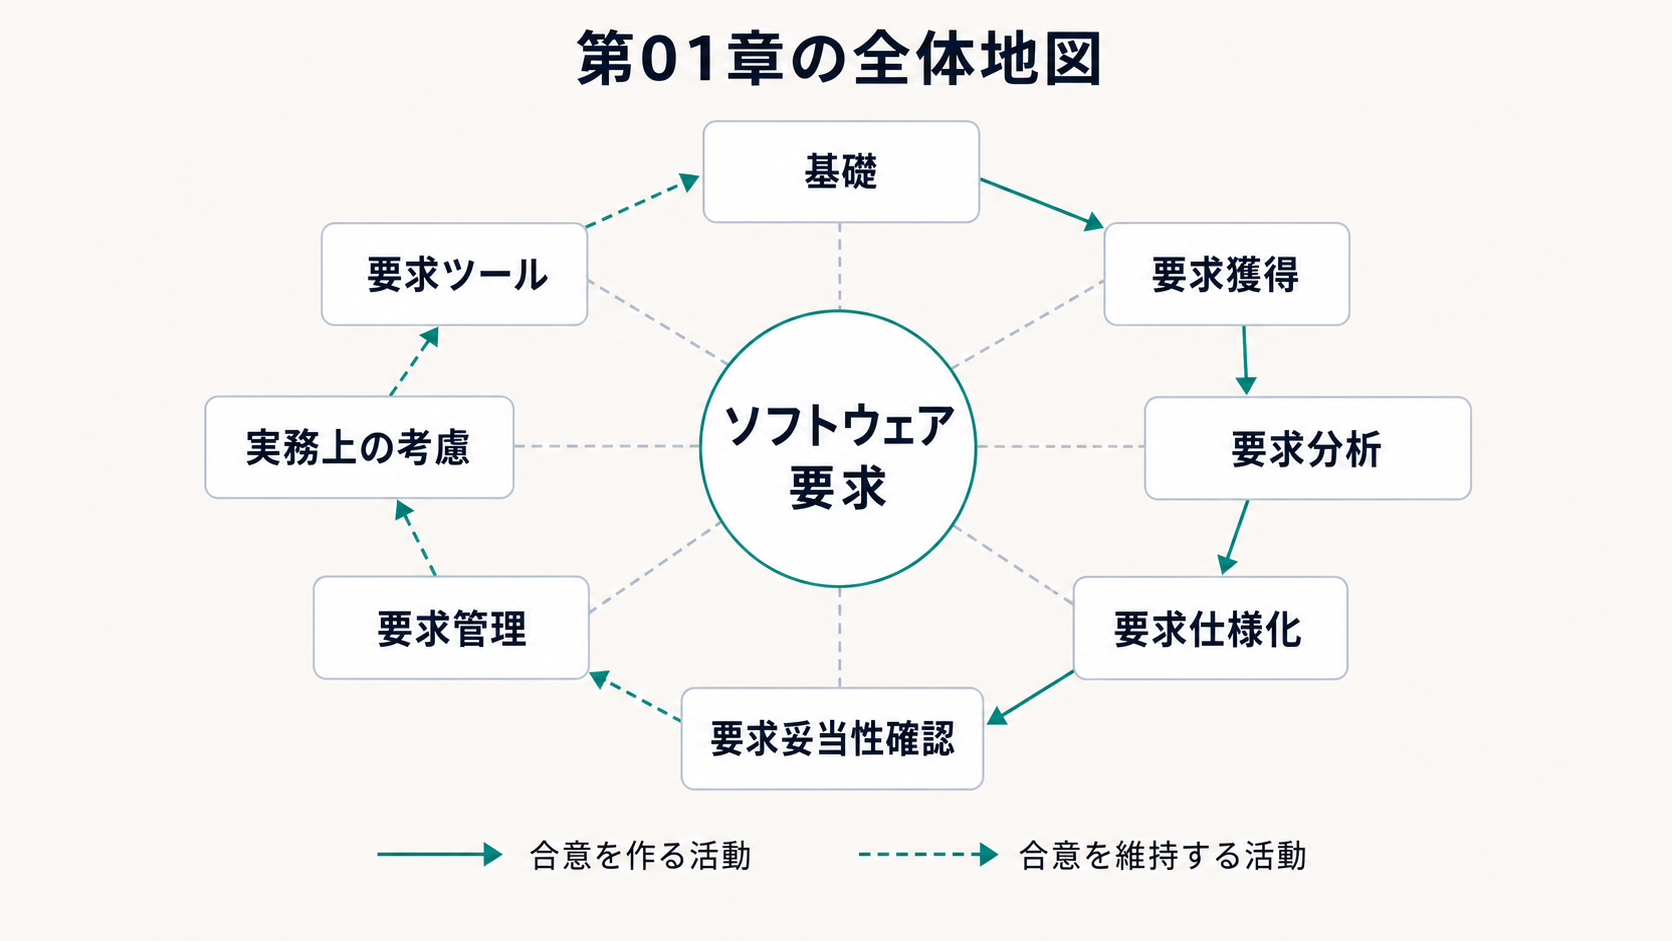
\includegraphics[width=0.96\linewidth]{assets/generated_figures/ch01/fig-ch01-01.png}}{\fbox{\parbox[c][48mm][c]{0.9\linewidth}{\centering 画像生成待ち\\第01章の全体地図}}}
\caption{第01章の全体地図}
\label{fig:ch01-01}
\end{figure}

\subsubsection*{最初に必要な用語}
\addcontentsline{toc}{subsubsection}{最初に必要な用語}

\par\smallskip\noindent\refstepcounter{table}\label{tab:ch01-01}\textbf{表 \thetable: 第01章 ソフトウェア要求 表01}\par\smallskip
\begin{tabularx}{0.97\linewidth}{@{}p{.25\linewidth}X@{}}
\toprule
用語 & 初学者向けの説明 \\
\midrule
\term{ソフトウェア} & プログラムだけでなく、データ、設定、操作手順、関連文書を含むことがある。 \\
\term{要求} & 何かを達成するために満たすべき条件・能力・制約。 \\
\term{利害関係者} & 開発結果に影響を与える、または影響を受ける人・組織。顧客、利用者、運用担当、規制当局など。 \\
\term{システム} & ソフトウェア、ハードウェア、人、手順、設備などが組み合わさって目的を達成するもの。 \\
\term{仕様} & 要求や設計などを、関係者が共有できるように記録したもの。 \\
\term{妥当性確認} & 「これを作れば本当に相手の問題を解決できるか」を確認すること。 \\
\term{追跡可能性} & 要求が設計、コード、テスト、利用者文書などとどうつながるかをたどれること。 \\
\bottomrule
\end{tabularx}

\subsection*{導入：要求が重要な理由}
\addcontentsline{toc}{subsection}{導入：要求が重要な理由}

ソフトウェア要求は、二つの視点から理解する。第一に、要求は「ソフトウェア製品やプロジェクトに対するニーズと制約の表現」である。第二に、要求は「そのニーズと制約を作り、保ち、変化に対応する活動」である。

要求を誤ると、プロジェクトの費用、納期、品質に大きく影響する。ひとつの要求は複数の設計判断を生み、ひとつの設計判断は複数のコード判断を生み、さらに複数のテスト判断につながる。したがって、要求の欠落や誤解が後工程で見つかると、修正範囲が連鎖的に広がる。

現実のプロジェクトで特に多い問題は、\term{不完全性}と\term{曖昧性}である。不完全性とは、必要な要求や詳細が明らかになっていない状態である。曖昧性とは、同じ要求文を複数の意味に解釈できる状態である。どちらも、作ったものが「本来ほしかったもの」とずれる原因になる。

要求文書は、初期開発のためだけではない。保守担当者が後からコードを見ると、コードが「何をしているか」は実行や解析でわかる場合がある。しかし、コードが「何を意図しているか」は要求がなければわかりにくい。欠陥とは、多くの場合、ソフトウェアが意図されたことと実際にしていることの差である。要求は、その意図を長期にわたって伝える役割を持つ。

\MiniBox{重要}{要求活動は、開発の最初に一回だけ行う作業ではない。要求は、プロジェクト開始時に始まり、開発中に洗練され、運用・保守の期間にも参照・変更される。}

\subsection{ソフトウェア要求の基礎}

\subsubsection{ソフトウェア要求の定義}

\term{ソフトウェア要求}とは、利用者が問題を解決したり目的を達成したりするために必要な条件または能力である。また、契約、標準、仕様、法令などを満たすために、システムや構成要素が備えるべき条件または能力でもある。さらに、それらを文書やモデルとして表したものも要求と呼ぶ。

より実務的に言えば、ソフトウェア要求とは「何を満たせば、現実世界の問題を解決したと言えるか」を表す合意である。ここでいう「問題」は、業務の自動化、既存ソフトウェアの欠点の修正、機器の制御、利用者体験の改善、規制への対応など、さまざまである。

\begin{definitionbox}ソフトウェア要求とは、ソフトウェアまたはソフトウェアを作るプロジェクトが満たすべき条件・能力・制約を、関係者が共有できるように表したものである。\end{definitionbox}

要求は通常、顧客、利用者、業務担当者から出る。しかし、それだけではない。規制当局、標準、既存システム、運用部門、サポート部門、開発組織、プロジェクト計画そのものも要求の源泉になる。

\subsubsection{ソフトウェア要求の分類}

要求は、すべてをひとまとめにすると扱いにくい。SWEBOKでは、ソフトウェア要求を大きく次のように整理する。

\begin{center}
\footnotesize
\par\smallskip\noindent\refstepcounter{table}\label{tab:ch01-02}\textbf{表 \thetable: 第01章 ソフトウェア要求 表02}\par\smallskip
\begin{tabular}{c}
ソフトウェア要求 \\
$\downarrow$ \\
ソフトウェア製品要求 \quad / \quad ソフトウェアプロジェクト要求 \\
$\downarrow$ \\
機能要求 \quad / \quad 非機能要求 \\
$\downarrow$ \\
技術制約 \quad / \quad サービス品質制約
\end{tabular}
\end{center}

\begin{figure}[htbp]
\centering
\IfFileExists{assets/generated_figures/ch01/fig-ch01-02.png}{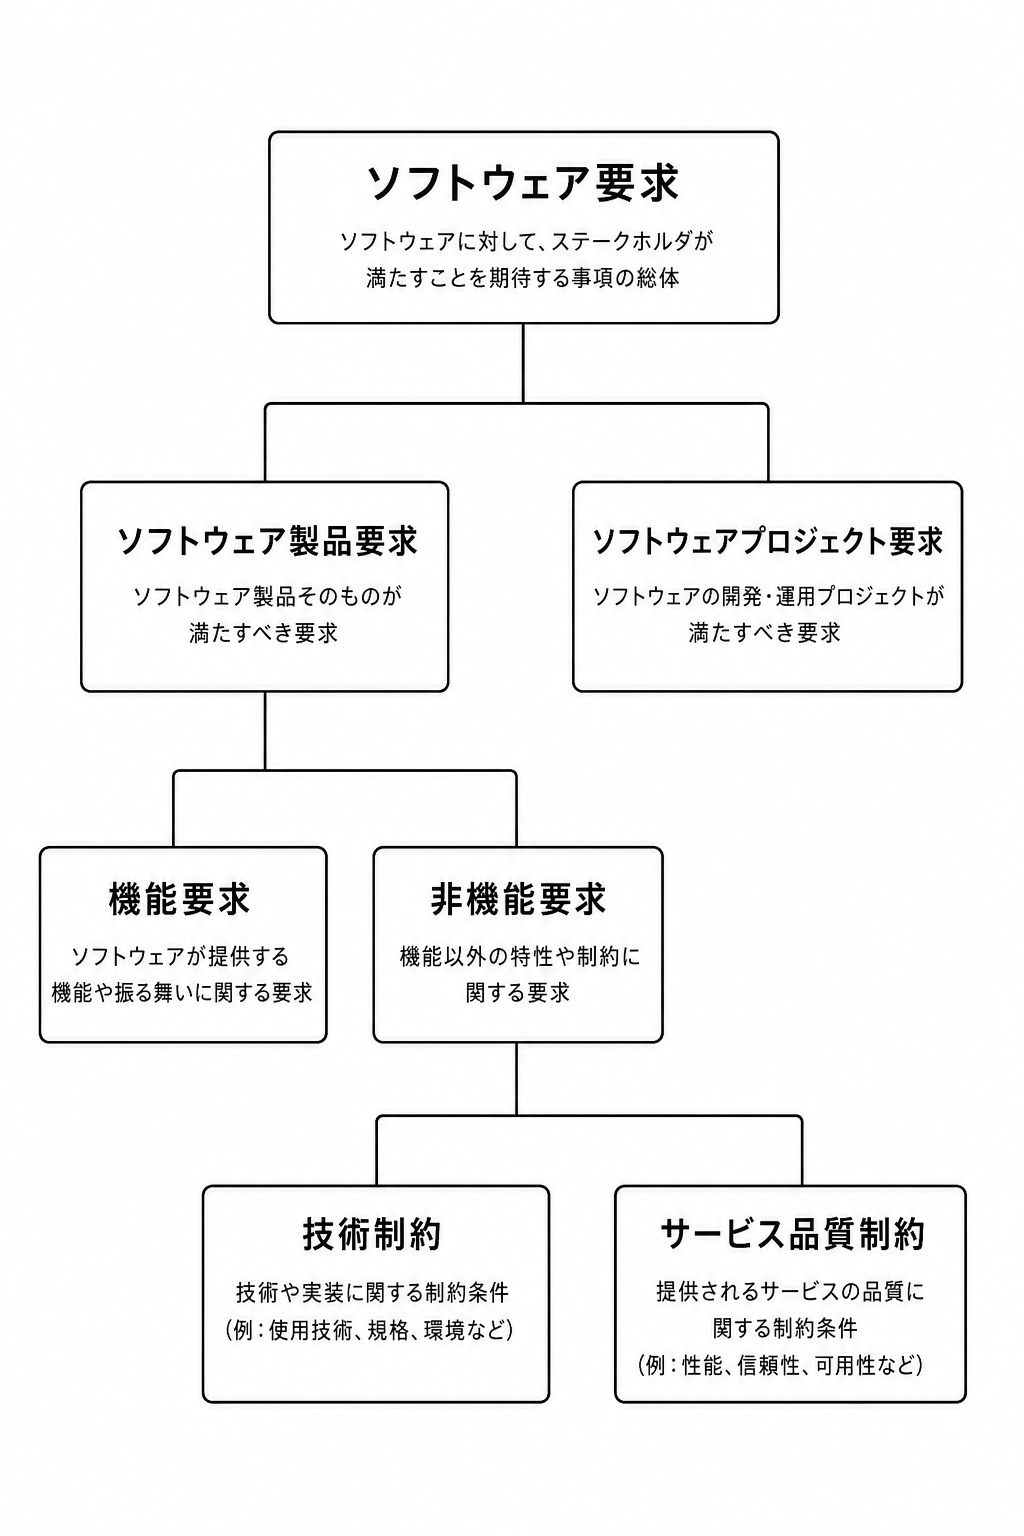
\includegraphics[width=0.96\linewidth]{assets/generated_figures/ch01/fig-ch01-02.png}}{\fbox{\parbox[c][48mm][c]{0.9\linewidth}{\centering 画像生成待ち\\要求分類の階層図}}}
\caption{要求分類の階層図}
\label{fig:ch01-02}
\end{figure}

分類の目的は、単に用語を覚えることではない。分類すると、要求の源泉、引き出し方、分析方法、仕様化の方法、確認すべき相手が見えやすくなる。

\subsubsection{ソフトウェア製品要求とソフトウェアプロジェクト要求}

\term{ソフトウェア製品要求}は、完成するソフトウェアそのものが満たすべき性質である。画面、処理、データ、外部連携、性能、信頼性、セキュリティなどが含まれる。

\term{ソフトウェアプロジェクト要求}は、ソフトウェアを作るプロジェクトの進め方を制約する要求である。費用、納期、人員、テスト環境、データ移行、利用者教育、保守準備などが例である。プロジェクト要求は、プロジェクト憲章、契約、計画書などに記録されることが多い。

\par\smallskip\noindent\refstepcounter{table}\label{tab:ch01-03}\textbf{表 \thetable: 第01章 ソフトウェア要求 表03}\par\smallskip
\begin{tabularx}{0.97\linewidth}{@{}p{.28\linewidth}X@{}}
\toprule
区分 & 見分け方 \\
\midrule
\term{製品要求} & 完成したソフトウェアがどう振る舞うか、どの品質を満たすかを述べる。 \\
\term{プロジェクト要求} & 開発の費用、納期、人員、進め方、移行、教育などを縛る。 \\
\bottomrule
\end{tabularx}

\MiniBox{例}{「利用者は注文履歴を検索できる」は製品要求である。「本番移行は年度末までに完了する」はプロジェクト要求である。}

\subsubsection{機能要求}

\term{機能要求}とは、ソフトウェアが提供すべき観測可能な振る舞いを表す要求である。言い換えると、「ソフトウェアが何をするか」を述べる要求である。

機能要求は、二つの観点で理解しやすい。第一に、\term{方針}である。方針とは、常に守られるべき規則である。たとえば銀行システムでは、「口座は少なくとも一人の所有者を持つ」「口座残高は負にならない」といった要求が該当する。第二に、\term{プロセス}である。プロセスとは、実行される業務手続きである。入金、出金、振込、予約、取消、検索、承認などが該当する。

\begin{definitionbox}機能要求とは、ソフトウェアが実行すべき処理、守るべき業務規則、利用者に提供すべき振る舞いを述べる要求である。\end{definitionbox}

\subsubsection{非機能要求}

\term{非機能要求}とは、ソフトウェアの実装技術や運用品質を制約する要求である。「何をするか」ではなく、「どのような条件で、どの水準で、どの技術的制約のもとで実現するか」に関わる。

非機能要求には、性能、応答時間、信頼性、正確性、可用性、拡張性、保存容量、プラットフォーム、利用するデータベースなどが含まれる。非機能要求はさらに、\term{技術制約}と\term{サービス品質制約}に分けると理解しやすい。

\MiniBox{注意}{「非機能要求」は「重要でない要求」という意味ではない。むしろ、性能、信頼性、セキュリティ、安全性など、失敗したときの影響が大きい要求が多い。}

\subsubsection{技術制約}

\term{技術制約}とは、特定の自動化技術やインフラを使うこと、または使わないことを指定する要求である。ここでは「名前のある技術を指定しているか」に注目すると見分けやすい。

\par\smallskip\noindent\refstepcounter{table}\label{tab:ch01-04}\textbf{表 \thetable: 第01章 ソフトウェア要求 表04}\par\smallskip
\begin{tabularx}{0.97\linewidth}{@{}p{.25\linewidth}X@{}}
\toprule
対象 & 例 \\
\midrule
プラットフォーム & Windows、macOS、Android、iOS など。 \\
プログラミング言語 & Java、C++、C\#、Python など。 \\
ブラウザ & Chrome、Safari、Edge など。 \\
データベース & Oracle、SQL Server、MySQL など。 \\
禁止事項 & ポインタ利用禁止、特定暗号方式の禁止、外部クラウド利用禁止など。 \\
\bottomrule
\end{tabularx}

技術制約は、既存システムとの連携、組織標準、保守要員のスキル、セキュリティ方針、ライセンス方針などから生じることが多い。

\subsubsection{サービス品質制約}

\term{サービス品質制約}とは、特定の技術名を指定せず、ソフトウェアが達成すべき品質水準を表す要求である。サービス品質という表現は、利用者や運用者が受け取るサービスの品質として考えるとわかりやすい。

\par\smallskip\noindent\refstepcounter{table}\label{tab:ch01-05}\textbf{表 \thetable: 第01章 ソフトウェア要求 表05}\par\smallskip
\begin{tabularx}{0.97\linewidth}{@{}p{.26\linewidth}X@{}}
\toprule
品質水準 & 要求文の例 \\
\midrule
応答時間 & 通常時、検索結果を2秒以内に返す。 \\
スループット & 1分あたり1万件のイベントを処理する。 \\
正確性 & 金額計算は定められた丸め規則に従う。 \\
信頼性 & 月間稼働率99.9\%以上を維持する。 \\
拡張性 & 利用者数が10倍になっても構成変更で対応できる。 \\
セキュリティ & 権限のない利用者は個人情報を閲覧できない。 \\
\bottomrule
\end{tabularx}

\subsubsection{なぜこのように分類するのか}

要求を分類する理由は、実務上は非常に明確である。

\begin{itemize}
\item 要求の種類によって、要求の源泉が異なる。
\item 源泉が異なれば、聞き出し方も異なる。
\item 種類によって、分析方法、仕様化方法、確認すべき相手が異なる。
\item 要求の種類によって、設計・実装・テストへの影響が異なる。
\end{itemize}

さらに、分類は複雑さを下げる。業務規則を議論している最中に、同時にデータベース製品や処理速度を議論すると、論点が混ざる。機能要求、技術制約、サービス品質制約を分ければ、業務の専門家は業務の観点に集中でき、技術者は技術の観点に集中できる。

\MiniBox{完全技術フィルタ}{機能要求と非機能要求の境界が曖昧なときは、「無限に速く、記憶容量が無限で、費用がゼロで、故障しない理想的なコンピュータがあっても、その要求を書く必要があるか」と問う。必要なら機能要求である。不要なら、技術や品質に関する制約、つまり非機能要求である。}

\begin{figure}[htbp]
\centering
\IfFileExists{assets/generated_figures/ch01/fig-ch01-03.png}{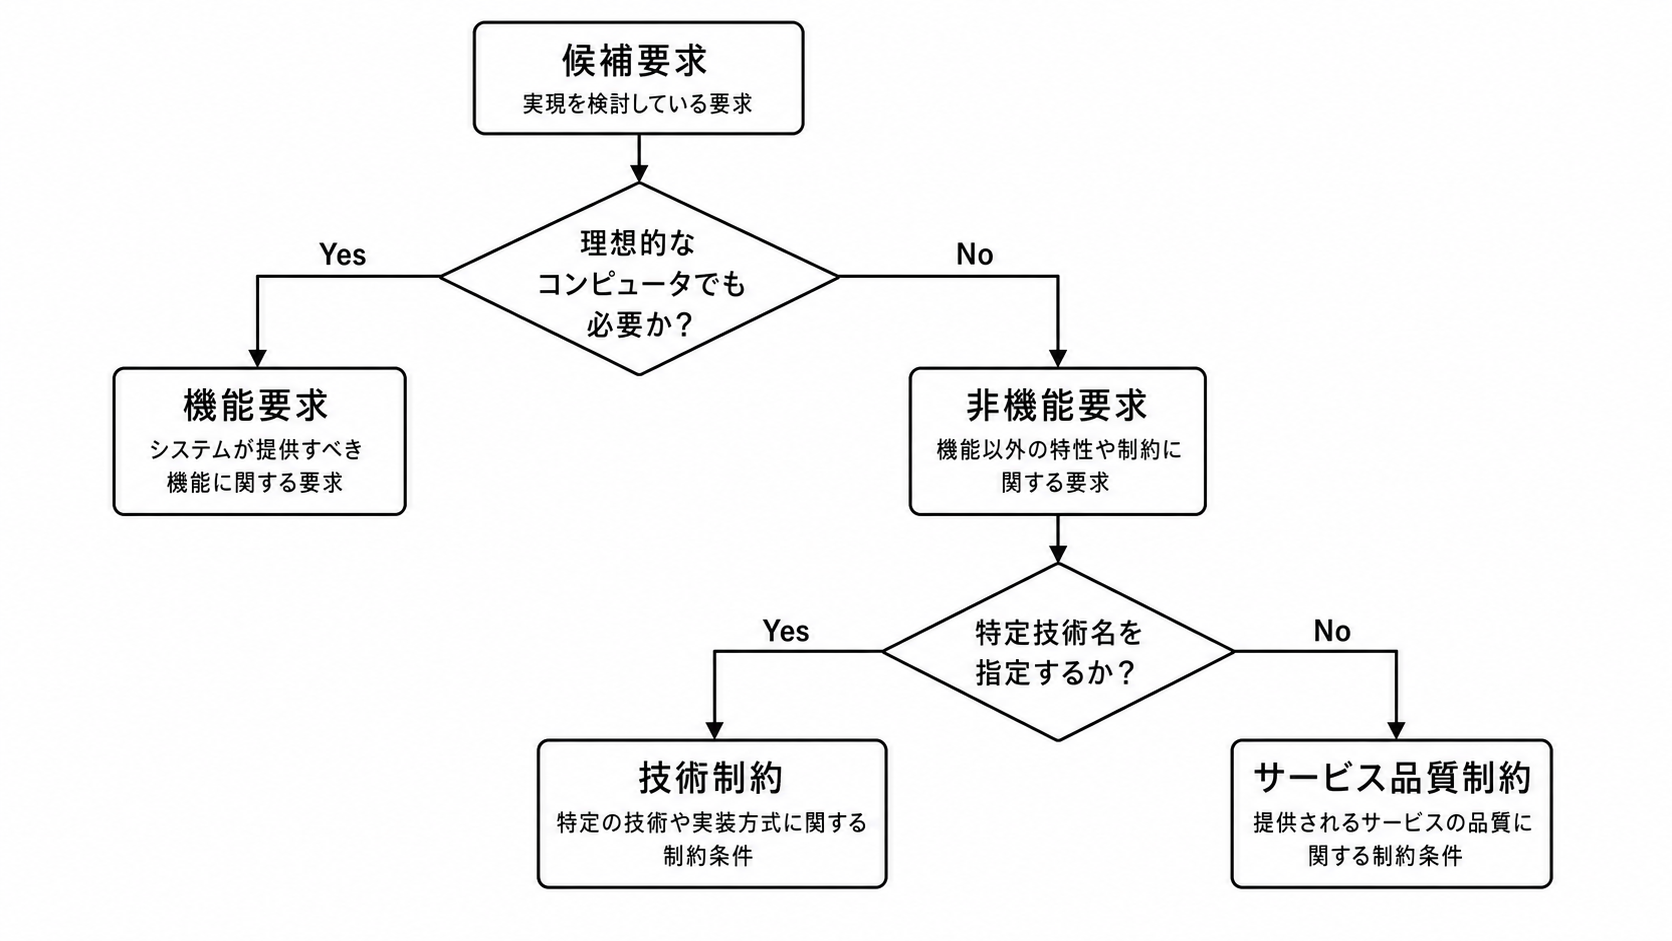
\includegraphics[width=0.96\linewidth]{assets/generated_figures/ch01/fig-ch01-03.png}}{\fbox{\parbox[c][48mm][c]{0.9\linewidth}{\centering 画像生成待ち\\完全技術フィルタの判定フロー}}}
\caption{完全技術フィルタの判定フロー}
\label{fig:ch01-03}
\end{figure}

\subsubsection{システム要求とソフトウェア要求}

\term{システム要求}は、ソフトウェアだけでなく、ハードウェア、ファームウェア、人、情報、手順、設備、サービス、支援要素を含むシステム全体に対する要求である。自動運転車、医療機器、工場制御、航空機システムのように、複数の要素が組み合わさる場合には、システム要求とソフトウェア要求を分けて扱うことが重要である。

\term{ソフトウェア要求}は、その大きなシステムの中で、ソフトウェア要素が満たすべき要求である。たとえば「車両は障害物を検知して安全に停止する」はシステム要求であり、その一部として「認識ソフトウェアは前方物体を一定時間内に分類する」といったソフトウェア要求が割り当てられる。

\begin{figure}[htbp]
\centering
\IfFileExists{assets/generated_figures/ch01/fig-ch01-04.png}{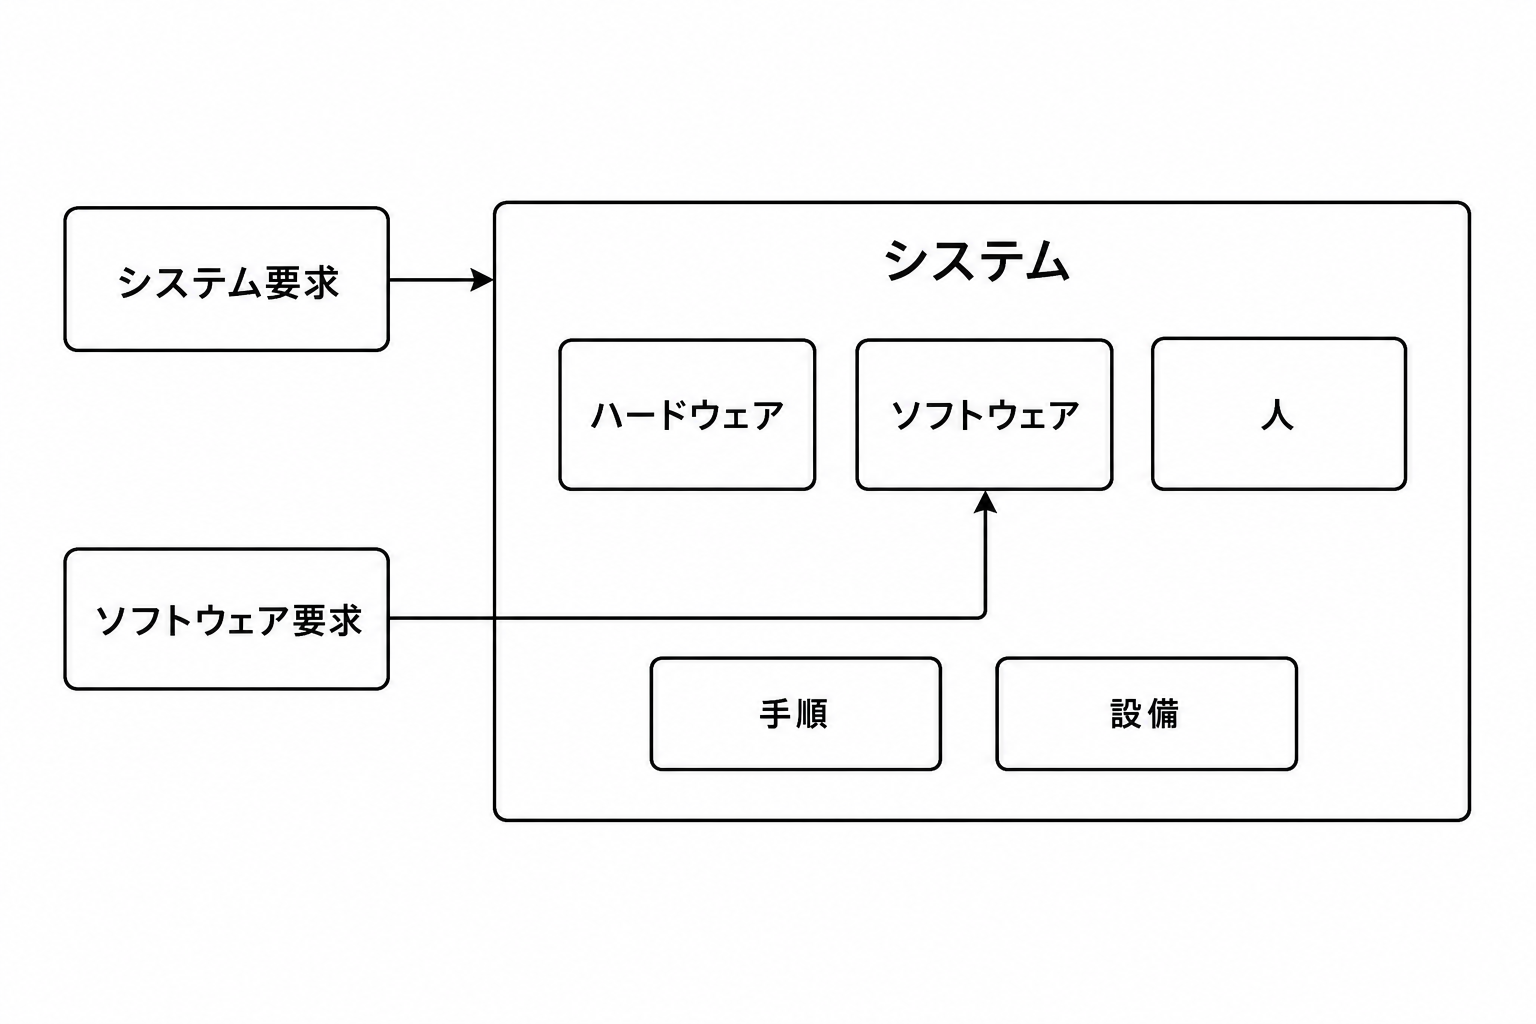
\includegraphics[width=0.96\linewidth]{assets/generated_figures/ch01/fig-ch01-04.png}}{\fbox{\parbox[c][48mm][c]{0.9\linewidth}{\centering 画像生成待ち\\システム要求からソフトウェア要求への割当図}}}
\caption{システム要求からソフトウェア要求への割当図}
\label{fig:ch01-04}
\end{figure}

\subsubsection{派生要求}

\term{派生要求}とは、外部の利害関係者から直接出された要求ではなく、開発チーム内部の判断から生まれ、下位チームや構成要素に課される要求である。

たとえば、アーキテクトが「パイプ・アンド・フィルタ構造を採用する」と決めたとする。この決定は、外部顧客から見ると設計判断である。しかし、個々のフィルタを作るサブチームから見ると、「この形式で入力を受け取り、この形式で出力する」という要求になる。このように、要求か設計かは視点に依存する。

\MiniBox{視点依存性}{同じ記述でも、上位の視点では設計判断、下位の視点では要求になることがある。要求とは「その作業を始める人にとって、満たさなければならない入力条件」として理解するとよい。}

\subsubsection{ソフトウェア要求活動}

要求活動は、大きく\term{要求開発}と\term{要求管理}に分けられる。

\term{要求開発}は、「何を作るか」について合意を作る活動である。具体的には、\term{要求獲得}、\term{要求分析}、\term{要求仕様化}、\term{要求妥当性確認}を含む。

\term{要求管理}は、その合意を時間とともに維持する活動である。要求は開発中にも保守中にも変化するため、不要な要求の整理、変更要求の扱い、スコープと予算・納期の調整が必要になる。

\begin{figure}[htbp]
\centering
\IfFileExists{assets/generated_figures/ch01/fig-ch01-05.png}{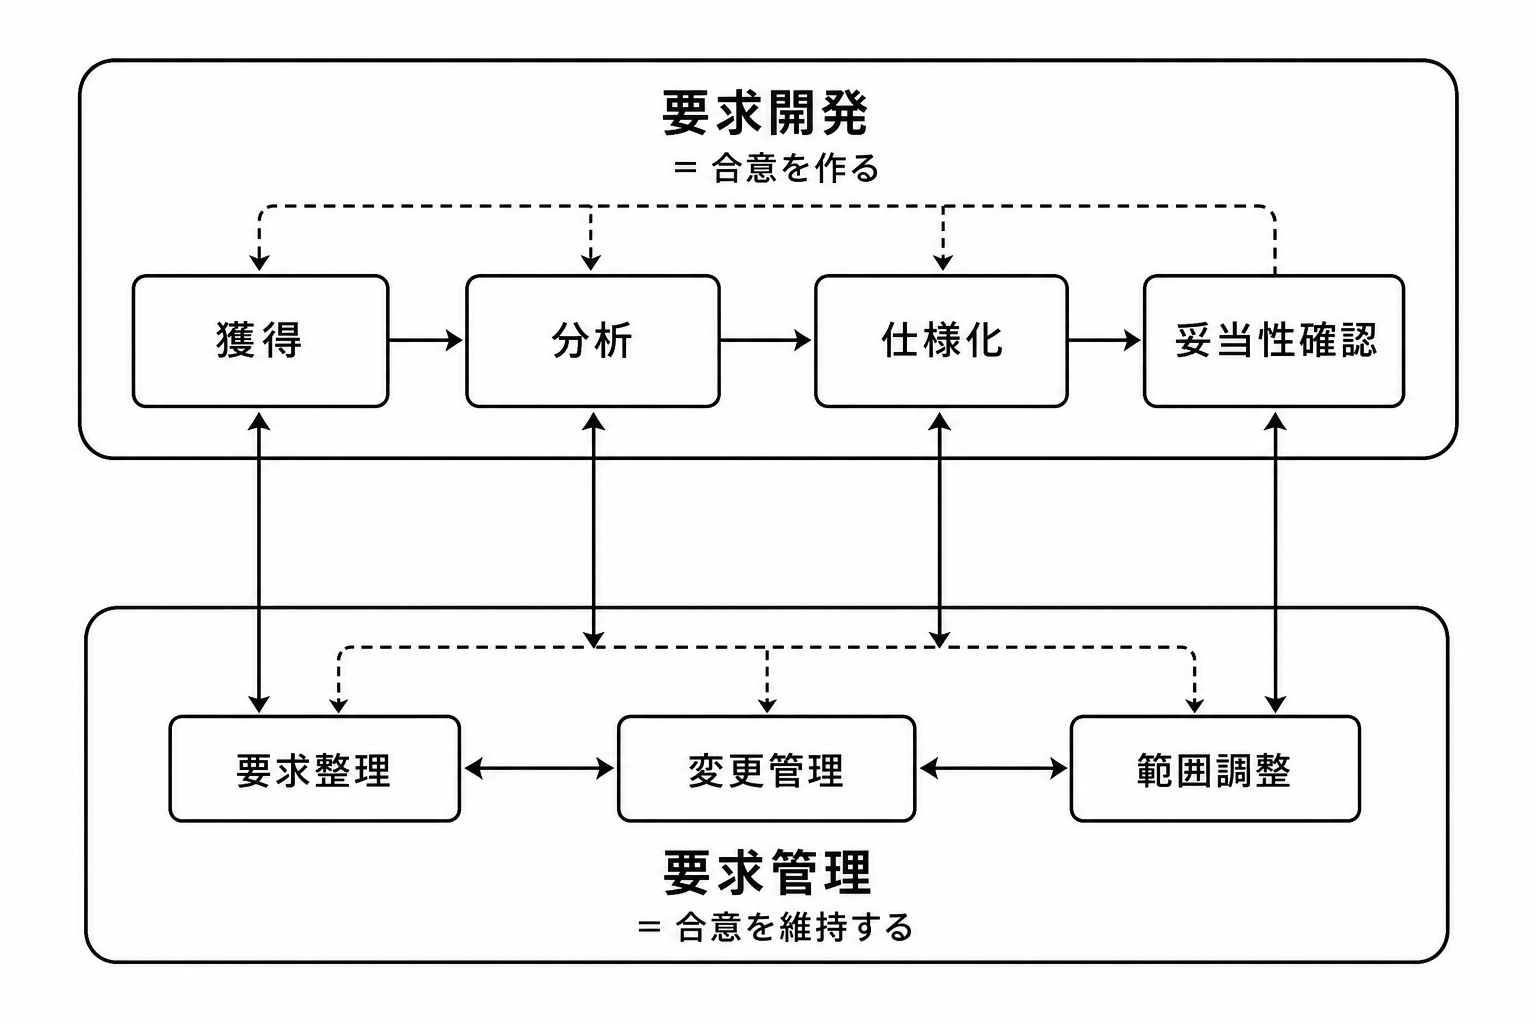
\includegraphics[width=0.96\linewidth]{assets/generated_figures/ch01/fig-ch01-05.png}}{\fbox{\parbox[c][48mm][c]{0.9\linewidth}{\centering 画像生成待ち\\要求開発と要求管理の活動図}}}
\caption{要求開発と要求管理の活動図}
\label{fig:ch01-05}
\end{figure}

\subsection{要求獲得}

\term{要求獲得}とは、候補となる要求を表面化させる活動である。英語では \,\en{Requirements Elicitation}\, と呼ばれる。直訳すれば「引き出し」であり、相手が最初から明確に言語化できるとは限らないニーズを、質問、観察、試作、資料調査などで明らかにする活動である。

要求獲得が不十分だと、不完全な要求が残る。完全性を保証することは難しいが、適切な源泉を見つけ、複数の技法を組み合わせることで、不完全性を減らせる。

\subsubsection{要求の源泉}

要求は多くの源泉から来る。人に由来する源泉と、人以外に由来する源泉の両方を考える必要がある。

\par\smallskip\noindent\refstepcounter{table}\label{tab:ch01-06}\textbf{表 \thetable: 第01章 ソフトウェア要求 表06}\par\smallskip
\begin{tabularx}{0.97\linewidth}{@{}p{.27\linewidth}X@{}}
\toprule
源泉 & 例 \\
\midrule
\term{顧客} & ソフトウェア開発に費用を出す人・組織。 \\
\term{利用者} & ソフトウェアを直接または間接に使う人。利用頻度、権限、熟練度で分類できる。 \\
\term{業務専門家} & 対象業務、規制、現場作業に詳しい人。 \\
\term{運用担当} & 本番環境、監視、障害対応、バックアップなどに責任を持つ人。 \\
\term{サポート担当} & 利用者からの問い合わせや障害報告を受ける人。 \\
\term{規制当局・専門団体} & 法令、標準、ガイドラインを通じて要求を課す組織。 \\
\term{開発者} & 技術的制約、保守性、開発効率に関する要求を示すことがある。 \\
\bottomrule
\end{tabularx}

また、要求は人からだけではなく、文書、既存システム、業務方針、計算環境、競合製品、障害履歴、標準、法規制からも得られる。

\MiniBox{利害関係者分析}{利害関係者分析とは、関係する人や組織をできるだけ漏れなく見つけ、代表性の偏りを減らす活動である。声の大きい利用者だけから要求を集めると、少数派や運用担当の重要な要求を見落としやすい。}

\subsubsection{要求獲得技法}

要求獲得には多くの技法がある。技法は相手や目的によって使い分ける。

\par\smallskip\noindent\refstepcounter{table}\label{tab:ch01-07}\textbf{表 \thetable: 第01章 ソフトウェア要求 表07}\par\smallskip
\begin{tabularx}{0.97\linewidth}{@{}p{.25\linewidth}X@{}}
\toprule
技法 & 何に向いているか \\
\midrule
\term{面接} & 個別の経験、例外処理、暗黙知を聞き出す。 \\
\term{会議・討議} & 複数の関係者で認識を合わせる。 \\
\term{促進付きワークショップ} & 利害関係者を集め、短時間で合意形成や要求整理を行う。 \\
\term{質問票・市場調査} & 多数の人から傾向を集める。 \\
\term{観察} & 現場作業や実際の利用状況を確認する。 \\
\term{徒弟型学習} & ソフトウェア技術者が実際の作業を体験し、暗黙知を得る。 \\
\term{試作} & 画面や操作感を具体化し、利用者から反応を得る。 \\
\term{ユーザーストーリーマッピング} & 利用者の行動の流れに沿って機能を整理する。 \\
\term{文献・標準調査} & 法規制、標準、既存仕様に基づく要求を見つける。 \\
\bottomrule
\end{tabularx}

\begin{figure}[htbp]
\centering
\IfFileExists{assets/generated_figures/ch01/fig-ch01-06.png}{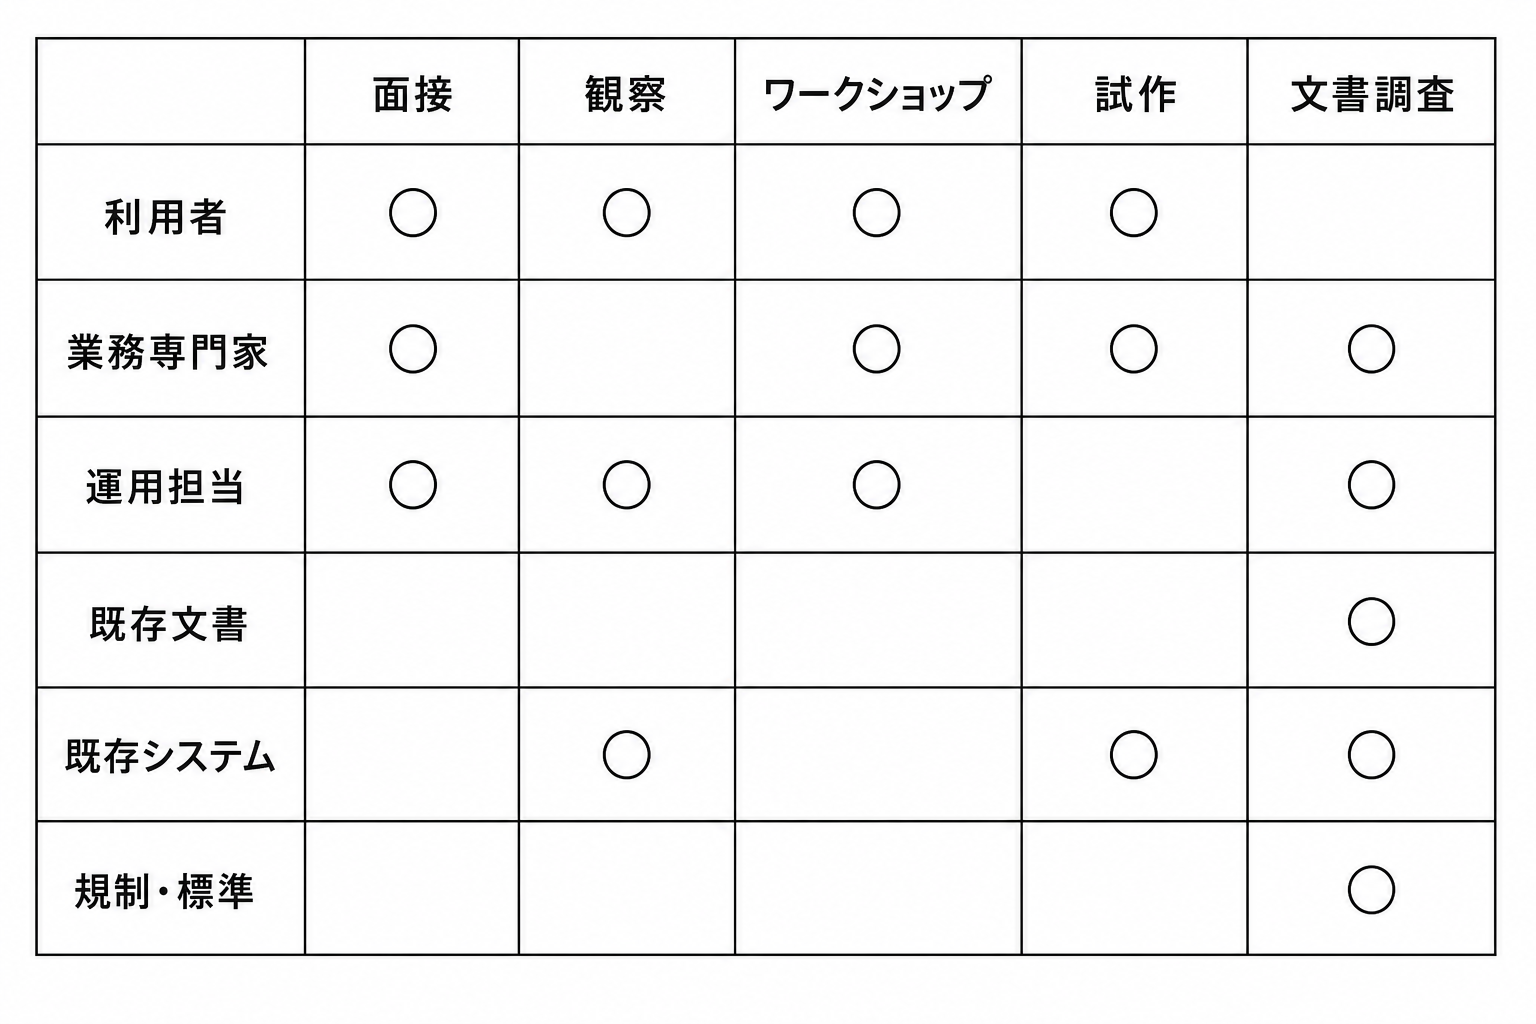
\includegraphics[width=0.96\linewidth]{assets/generated_figures/ch01/fig-ch01-06.png}}{\fbox{\parbox[c][48mm][c]{0.9\linewidth}{\centering 画像生成待ち\\要求の源泉と獲得技法の対応図}}}
\caption{要求の源泉と獲得技法の対応図}
\label{fig:ch01-06}
\end{figure}

要求獲得は受け身の活動ではない。利用者は自分の作業をうまく説明できないことがある。重要な情報を当然のこととして言わないこともある。したがって、技術者は「言われたことを書くだけ」ではなく、質問し、観察し、仮説を作り、確認する必要がある。

\subsection{要求分析}

\term{要求分析}とは、獲得された候補要求の意味、妥当性、矛盾、実現可能性、影響を調べる活動である。要求は、最初から完成形で出てくるとは限らない。多くの場合、曖昧、過剰、矛盾、不足、または解決策の断片として現れる。分析の目的は、それを真の要求へ近づけることである。

\subsubsection{要求の性質}

よい要求には、個々の要求として望ましい性質と、要求集合として望ましい性質がある。

\paragraph{個々の要求の望ましい性質}

\par\smallskip\noindent\refstepcounter{table}\label{tab:ch01-08}\textbf{表 \thetable: 第01章 ソフトウェア要求 表08}\par\smallskip
\begin{tabularx}{0.97\linewidth}{@{}p{.26\linewidth}X@{}}
\toprule
性質 & 説明 \\
\midrule
\term{一意に解釈できる} & 読む人によって意味が変わらない。 \\
\term{テスト可能である} & 満たしたかどうかを確認できる。必要なら数値で示す。 \\
\term{拘束力がある} & 顧客がそれに価値を認め、満たされないことを受け入れない。 \\
\term{原子的である} & 一つの要求が一つの判断だけを表す。 \\
\term{真のニーズを表す} & 単なる思いつきや特定解ではなく、実際の問題に基づく。 \\
\term{利害関係者の語彙を使う} & 利用者や業務専門家が理解できる言葉で書く。 \\
\term{関係者に受け入れられる} & 重要な利害関係者が納得できる。 \\
\bottomrule
\end{tabularx}

\paragraph{要求集合の望ましい性質}

\par\smallskip\noindent\refstepcounter{table}\label{tab:ch01-09}\textbf{表 \thetable: 第01章 ソフトウェア要求 表09}\par\smallskip
\begin{tabularx}{0.97\linewidth}{@{}p{.26\linewidth}X@{}}
\toprule
性質 & 説明 \\
\midrule
\term{完全性} & 通常ケースだけでなく、境界条件、例外条件、セキュリティ上の必要事項も扱う。 \\
\term{簡潔性} & 不要な記述や重複が少ない。 \\
\term{内部整合性} & 要求同士が矛盾しない。 \\
\term{外部整合性} & 契約、法令、標準、業務文書などの外部資料と矛盾しない。 \\
\term{実現可能性} & 費用、納期、人員、技術制約の範囲で実現できる。 \\
\bottomrule
\end{tabularx}

\MiniBox{5つのなぜ}{要求が解決策の形で出てきたときは、「なぜそれが必要なのか」を繰り返し問う。目的は、相手が本当に解決したい問題に到達することである。}

\subsubsection{サービス品質要求の経済性}

サービス品質制約は、単に「高ければよい」ものではない。たとえば、応答時間を極限まで短くする、稼働率を極限まで高くする、処理能力を極限まで大きくするには、費用が増える。したがって、要求は価値と費用の関係で考える必要がある。

\term{失敗点}は、それを下回るとシステムとして価値がほとんどなくなる水準である。\term{完全点}は、それを超えても利用者に追加価値がほとんど出ない水準である。現実的には、要求値はこの間で決まる。最もよい水準は、価値と費用の差が最大になる点である。

\begin{figure}[htbp]
\centering
\IfFileExists{assets/generated_figures/ch01/fig-ch01-07.png}{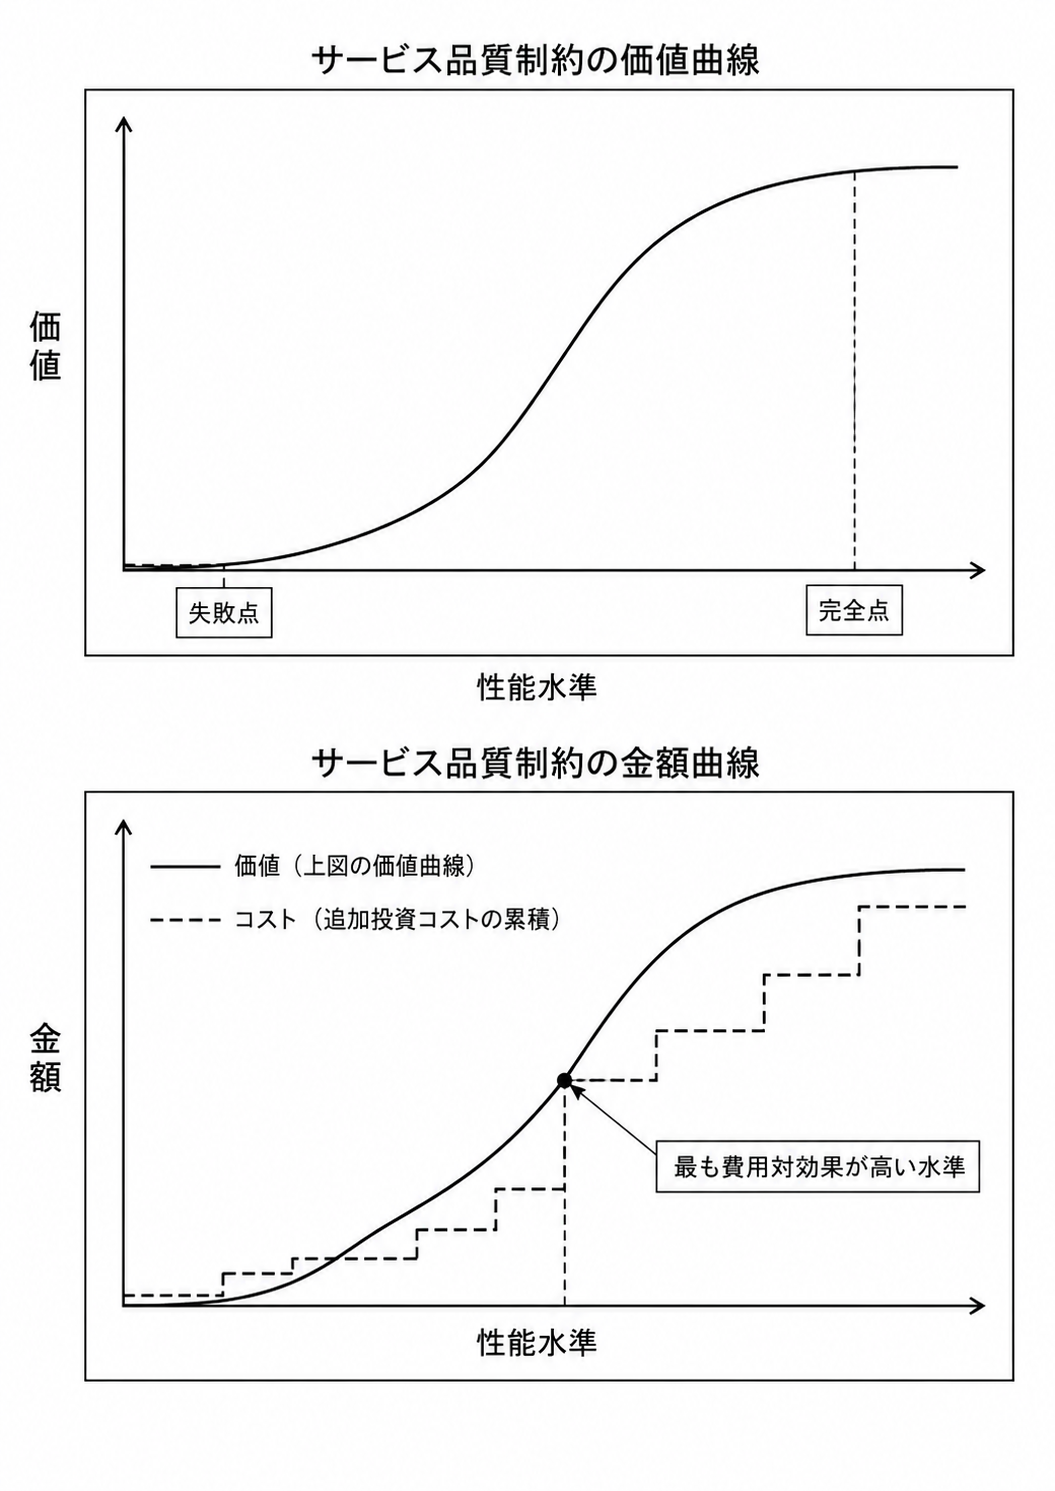
\includegraphics[width=0.96\linewidth]{assets/generated_figures/ch01/fig-ch01-07.png}}{\fbox{\parbox[c][48mm][c]{0.9\linewidth}{\centering 画像生成待ち\\サービス品質制約の価値・費用曲線}}}
\caption{サービス品質制約の価値・費用曲線}
\label{fig:ch01-07}
\end{figure}

サービス品質制約同士には、よい関係と悪い関係がある。たとえば、コードを単純にすると信頼性と変更容易性が同時に上がることがある。一方、実行速度を極端に高める最適化が、コードを複雑にして変更容易性を下げることもある。

\subsubsection{形式的分析}

\term{形式的分析}とは、数学的に意味が定義された言語やモデルを使って、要求を精密に表し、性質を検査する方法である。たとえば、デッドロックが起きないこと、特定の状態へ必ず到達すること、矛盾した状態が存在しないことなどを確認するために使われる。

形式的分析の利点は、曖昧さを減らせること、要求を論理的に推論できること、通常のレビューでは見落としやすい性質を確認できることである。一方で、記法を学ぶ負担があり、すべてのプロジェクトに適するわけではない。安全性や信頼性が非常に重要な領域で特に価値が高い。

\subsubsection{要求の衝突への対応}

利害関係者が多いほど、要求の衝突は起こりやすい。たとえば、利用者は高機能を求め、運用担当は単純で安定した運用を求め、経営側は費用や納期を抑えたいと考えることがある。

衝突への対応には、主に二つの方向がある。第一に、関係者間で交渉し、合意を形成することである。技術者が独断で決めると、責任や契約上の問題が残ることがある。第二に、\term{製品群開発}の考え方を使い、すべての利用者に共通する不変要求と、利用者や市場によって変わる可変要求を分けることである。

\MiniBox{例}{天気アプリで、ある利用者は摂氏表示を求め、別の利用者は華氏表示を求める。この場合、温度を表示することは共通要求であり、単位は可変要求である。}

\subsection{要求仕様化}

\term{要求仕様化}とは、要求を記録し、記憶し、伝達できる形にする活動である。仕様化の方法は一つではない。自然言語で書く、構造化したテンプレートで書く、受け入れ基準として書く、モデルで表すなど、複数の方法がある。

どの方法を選ぶかは、プロジェクトの性質によって変わる。業務領域への理解、リスクの大きさ、チームの地理的分散、外注の有無、契約上の要求、要求に基づくテストの必要性、保守期間中の担当者交代などを考慮する必要がある。

\MiniBox{基本方針}{要求仕様は、読む人を意識して作る。利用者、顧客、設計者、開発者、テスト担当、保守担当は、それぞれ必要とする情報が違う。}

\subsubsection{非構造化自然言語による要求仕様化}

\term{非構造化自然言語}とは、通常の文章で要求を書く方法である。たとえば「システムは、利用者が注文履歴を検索できるようにする」といった文である。

利点は、誰でも読み書きしやすいことである。欠点は、曖昧さや抜け漏れが発生しやすいことである。自然言語は柔軟であるため、同じ文が複数の意味に読めることがある。

\subsubsection{構造化自然言語による要求仕様化}

\term{構造化自然言語}とは、自然言語を使いながら、書き方に制約を加える方法である。代表例は、\term{主体・動作形式}である。「いつ」「誰が」「何をする」「どの条件で」という形にそろえると、曖昧さを減らせる。

\MiniBox{例}{「注文が出荷されたとき、システムは請求書を作成する。ただし、注文条件が前払いの場合を除く。」この文では、きっかけ、主体、動作、例外条件が明示されている。}

他にも、\term{ユースケース仕様}、\term{ユーザーストーリー}、\term{決定表}などが構造化自然言語の例である。ユーザーストーリーは、「ある役割として、ある能力がほしい。なぜなら、ある便益を得たいからである」という形式で、利用者視点の価値を表す。

\subsubsection{受け入れ基準に基づく要求仕様化}

\term{受け入れ基準}とは、要求が満たされたと判断するための条件である。要求を受け入れ基準の形で書くと、テストと要求が強く結びつく。

\term{受け入れテスト駆動開発}（ATDD）は、機能を作る前に、その機能が完成したと判断するテストを合意する方法である。\term{振る舞い駆動開発}（BDD）は、利用者の振る舞いを「前提、事象、結果」の形で書く方法である。

\MiniBox{BDDの例}{前提：口座残高が500円で、カードが有効である。事象：利用者が100円の出金を要求する。結果：ATMは100円を払い出し、口座残高は400円になる。}

この方法は、曖昧さの低減に有効である。一方で、どのシナリオを書くべきかを見落とすと不完全性は残る。そのため、境界値分析、組合せテスト、同値分割などのテスト技法と組み合わせるとよい。

\subsubsection{モデルに基づく要求仕様化}

\term{モデル}とは、複雑な対象を理解しやすくするために、必要な部分だけを抽象化して表したものです。要求仕様化では、文章だけでなく、図や形式的な記法を使って要求を表すことがある。UMLやSysMLの一部は、そのために使われる。

モデルは大きく二種類に分けられる。\term{構造モデル}は、概念、データ、関係、業務規則を表す。\term{振る舞いモデル}は、処理の流れ、利用者とのやり取り、状態遷移、イベントへの反応を表す。

\par\smallskip\noindent\refstepcounter{table}\label{tab:ch01-10}\textbf{表 \thetable: 第01章 ソフトウェア要求 表10}\par\smallskip
\begin{tabularx}{0.97\linewidth}{@{}p{.24\linewidth}X@{}}
\toprule
モデルの種類 & 例 \\
\midrule
構造モデル & クラス図、概念データモデル、実体関連図。 \\
振る舞いモデル & ユースケース図、シーケンス図、状態遷移図、活動図、データフロー図。 \\
\bottomrule
\end{tabularx}

モデルには、手描きのラフな図から、数学的意味を厳密に持つ形式モデルまで幅がある。形式性が高いほど曖昧さは減るが、作成と理解の負担は増える。

\begin{figure}[htbp]
\centering
\IfFileExists{assets/generated_figures/ch01/fig-ch01-08.png}{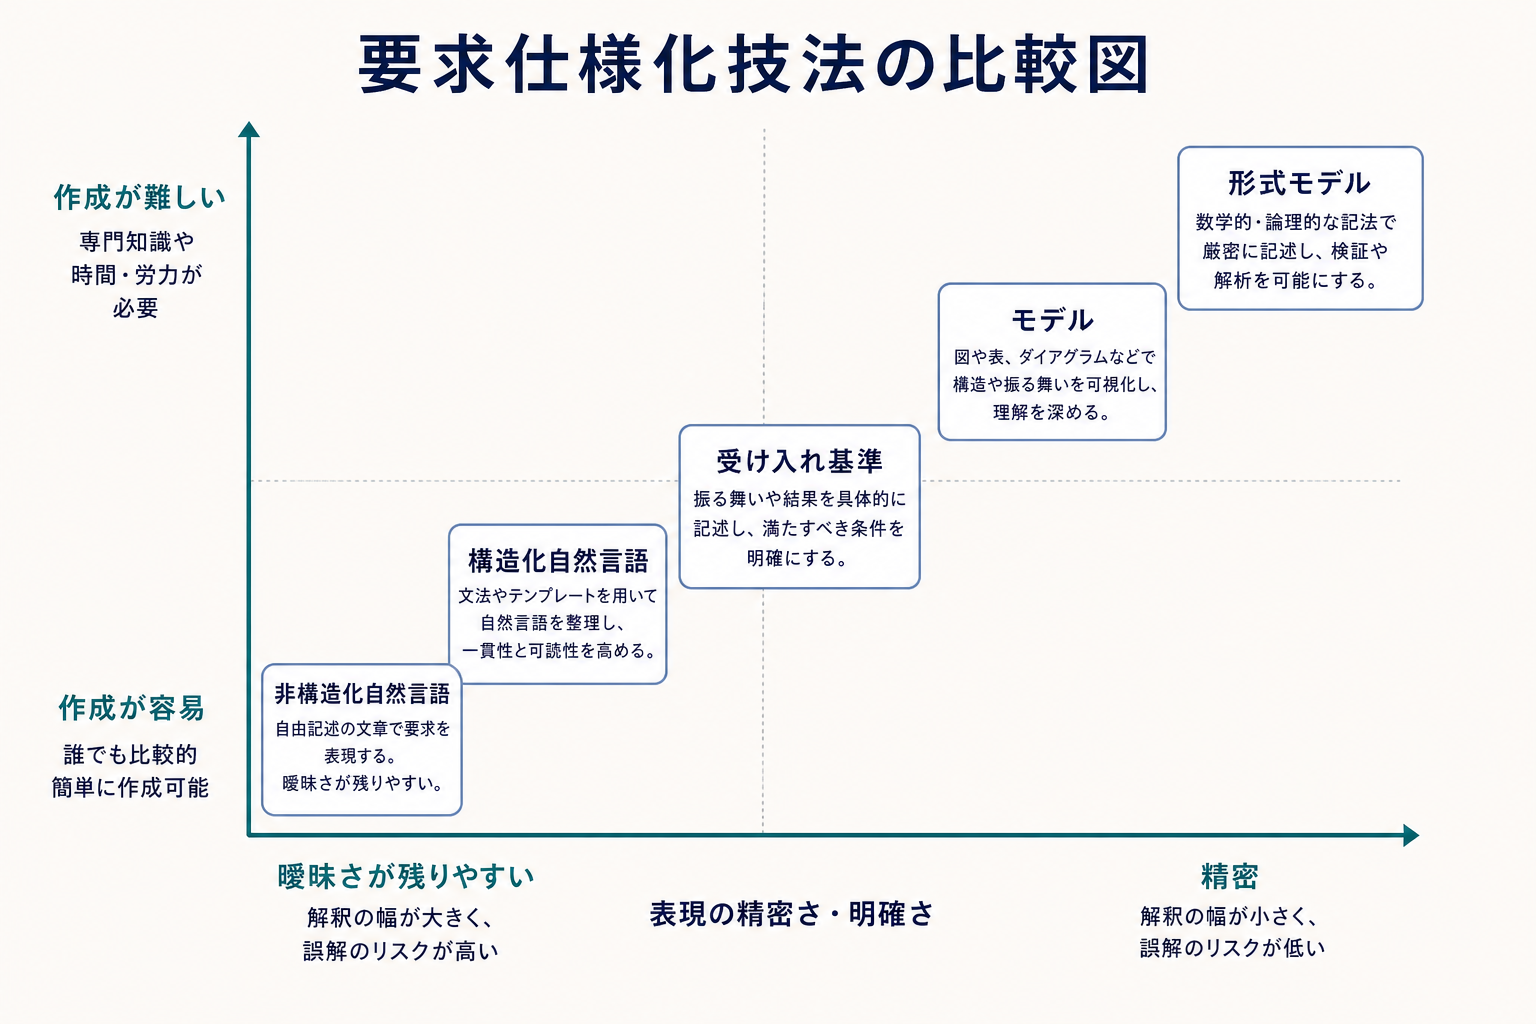
\includegraphics[width=0.96\linewidth]{assets/generated_figures/ch01/fig-ch01-08.png}}{\fbox{\parbox[c][48mm][c]{0.9\linewidth}{\centering 画像生成待ち\\要求仕様化技法の比較図}}}
\caption{要求仕様化技法の比較図}
\label{fig:ch01-08}
\end{figure}

\subsubsection{要求の追加属性}

要求文そのものに加えて、要求を管理するための属性を付けると有用である。

\par\smallskip\noindent\refstepcounter{table}\label{tab:ch01-11}\textbf{表 \thetable: 第01章 ソフトウェア要求 表11}\par\smallskip
\begin{tabularx}{0.97\linewidth}{@{}p{.25\linewidth}X@{}}
\toprule
属性 & 目的 \\
\midrule
識別子 & 要求を一意に参照し、追跡する。 \\
説明 & 要求文だけでは足りない背景を補足する。 \\
根拠 & なぜその要求が必要かを説明する。 \\
源泉 & 誰または何から出た要求かを示す。 \\
種類 & 機能要求、技術制約、サービス品質制約などを示す。 \\
依存関係 & 他の要求との前後関係や依存を示す。 \\
衝突 & 他の要求と矛盾する可能性を示す。 \\
受け入れ基準 & 完了判定に使う条件を示す。 \\
優先度 & 重要度や実施順序を示す。 \\
安定性 & 変更される可能性を示す。 \\
変更履歴 & いつ、誰が、なぜ変更したかを残す。 \\
\bottomrule
\end{tabularx}

\subsubsection{増分的仕様化と包括的仕様化}

要求を明示的に文書化するプロジェクトでは、\term{増分的仕様化}と\term{包括的仕様化}の二つの考え方がある。

増分的仕様化では、今回の版で追加・変更・削除された差分だけを記録する。文書量は小さくなりやすいが、全体像を理解するには過去の差分を追う必要がある。

包括的仕様化では、各版にすべての要求を含める。文書量は増えるが、その版だけで全体を理解できる。実務では、マイナー版は差分、メジャー版は包括的に書くという組合せもある。

\subsection{要求妥当性確認}

\term{要求妥当性確認}とは、現在理解されている要求が、利害関係者の真のニーズを表しているかを確認する活動である。英語では \,\en{Requirements Validation}\, と呼ばれる。

ここで大切なのは、「正しく書かれているか」だけではなく、「そもそもこれを作れば問題が解決するか」を見ることである。要求文が文法的に正しくても、利用者の実際の困りごとを解決しないなら妥当ではない。

\MiniBox{妥当性確認で問うこと}{要求はこの時点で必要なものを十分に含んでいるか。不要な要求はないか。理解しやすいか。矛盾していないか。標準や契約に合っているか。}

\subsubsection{要求レビュー}

\term{要求レビュー}は、要求文書やモデルを人が読んで確認する方法である。もっとも一般的な妥当性確認手段である。

レビューには複数の視点が必要である。顧客や利用者は、自分たちのニーズが正しく表されているかを見る。要求の専門家は、文書が明確で、標準に沿っているかを見る。設計者や開発者は、設計・実装に必要な情報があるかを見る。テスト担当は、テスト可能かを見る。

\subsubsection{シミュレーションと実行}

形式的またはモデルベースの要求仕様では、仕様を手作業またはツールで\term{実行}または\term{シミュレーション}できることがある。利用者は、文章を読むよりも、シナリオに沿って動く様子を見る方が理解しやすい場合がある。

\subsubsection{プロトタイピング}

\term{プロトタイプ}とは、本格的な実装の前に作る試作品である。画面の動き、操作感、処理の流れ、重要な技術的可能性などを具体的に示すために使う。

プロトタイプは、技術者の解釈を利害関係者に見せ、誤解を早く発見するのに有効である。ただし、見た目の細部や一時的な品質問題に関心が向きすぎると、本来確認したい要求から注意がそれることがある。

\begin{figure}[htbp]
\centering
\IfFileExists{assets/generated_figures/ch01/fig-ch01-09.png}{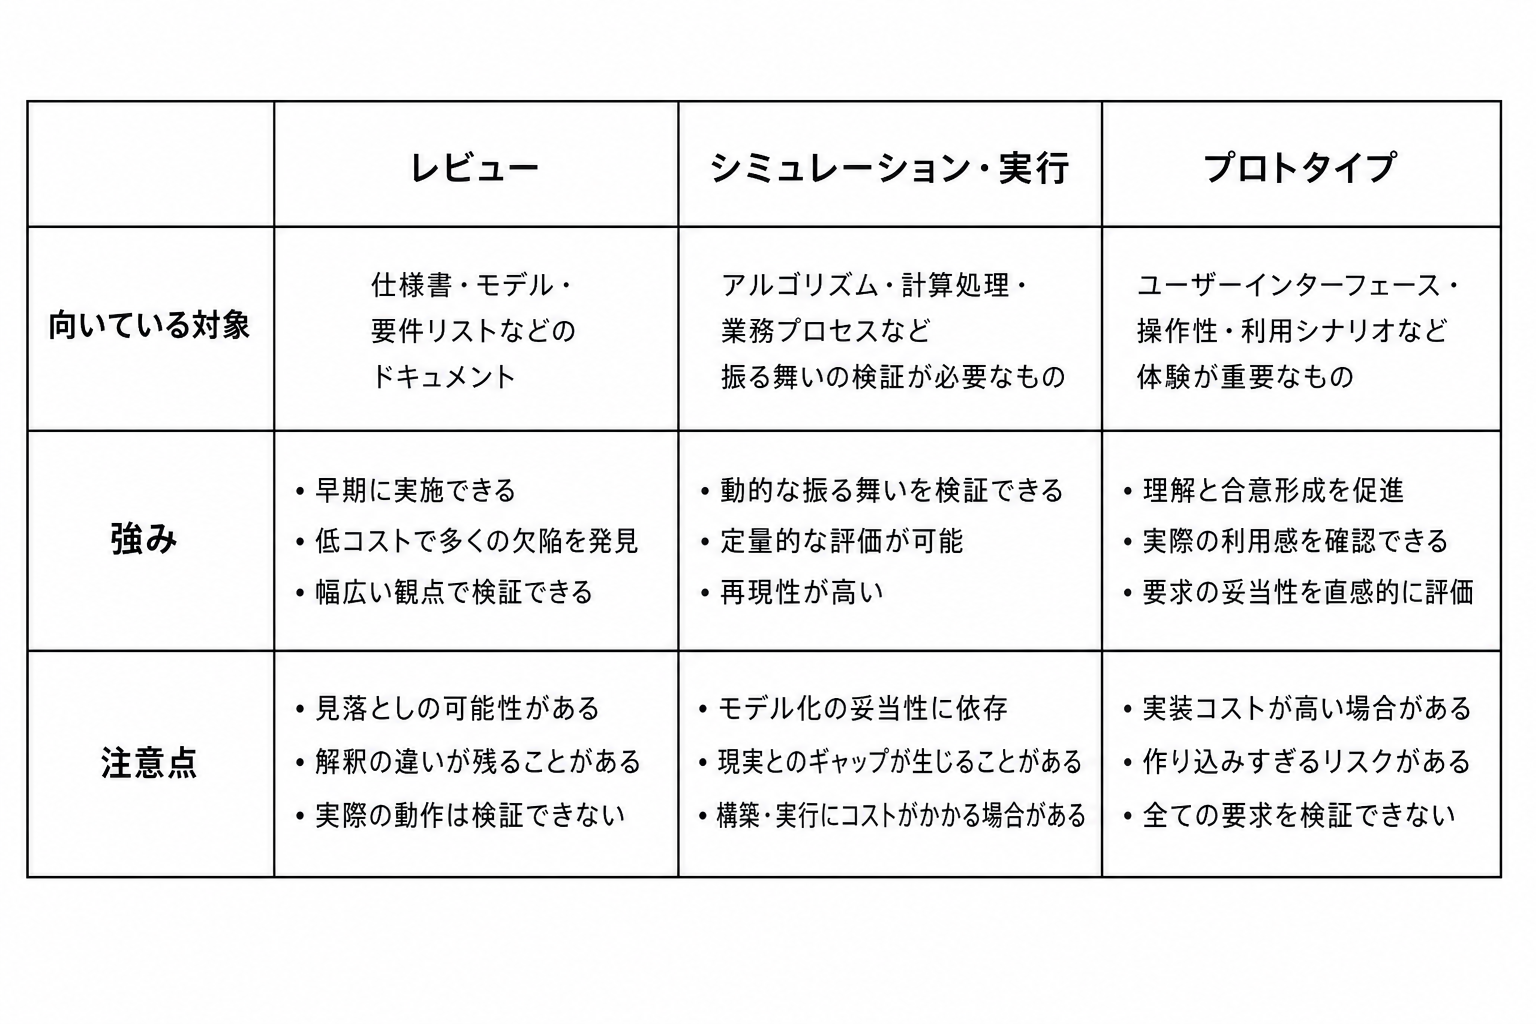
\includegraphics[width=0.96\linewidth]{assets/generated_figures/ch01/fig-ch01-09.png}}{\fbox{\parbox[c][48mm][c]{0.9\linewidth}{\centering 画像生成待ち\\要求妥当性確認の三手法を比較する図}}}
\caption{要求妥当性確認の三手法を比較する図}
\label{fig:ch01-09}
\end{figure}

\subsection{要求管理活動}

要求開発が「合意を作る活動」だとすれば、\term{要求管理}は「合意を維持する活動」である。要求は開発中にも保守中にも変わる。したがって、不要な要求を減らし、変更を統制し、範囲と制約を整合させる必要がある。

\subsubsection{要求整理・削減}

\term{要求整理・削減}は、英語の \,\en{Requirements Scrubbing}\, に対応する。目的は、利害関係者のニーズを満たすために必要な、できるだけ小さく、単純な要求集合を得ることである。

削減の対象は、範囲外の要求、費用対効果が低い要求、重要度が低い要求、過度に複雑な要求である。要求が減れば、設計、実装、テスト、保守の負担も減る。

\subsubsection{要求変更管理}

\term{要求変更管理}とは、合意済みの要求を変更する手順を管理する活動である。計画駆動型の開発では、変更要求、影響分析、承認・却下・保留の判断、関係者への通知、完了までの追跡が明示的に行われることが多い。

アジャイル型の開発では、変更要求がプロダクトバックログの項目として扱われ、優先度が高くなったときに反復に取り込まれることが多い。どちらの場合も、変更を受け入れるとは、納期、費用、人員、または他の範囲への影響を受け入れることを意味する。

\subsubsection{範囲調整}

\term{範囲調整}とは、作るべき要求の範囲が、費用、納期、人員などの制約を超えないように調整する活動である。範囲が大きすぎる場合には、要求を減らす、予算や人員を増やす、納期を延ばす、またはそれらを組み合わせる必要がある。

可能であれば、範囲調整は感覚ではなく、機能規模、工数、リスクなどの測定値に基づいて行うとよい。

\begin{figure}[htbp]
\centering
\IfFileExists{assets/generated_figures/ch01/fig-ch01-10.png}{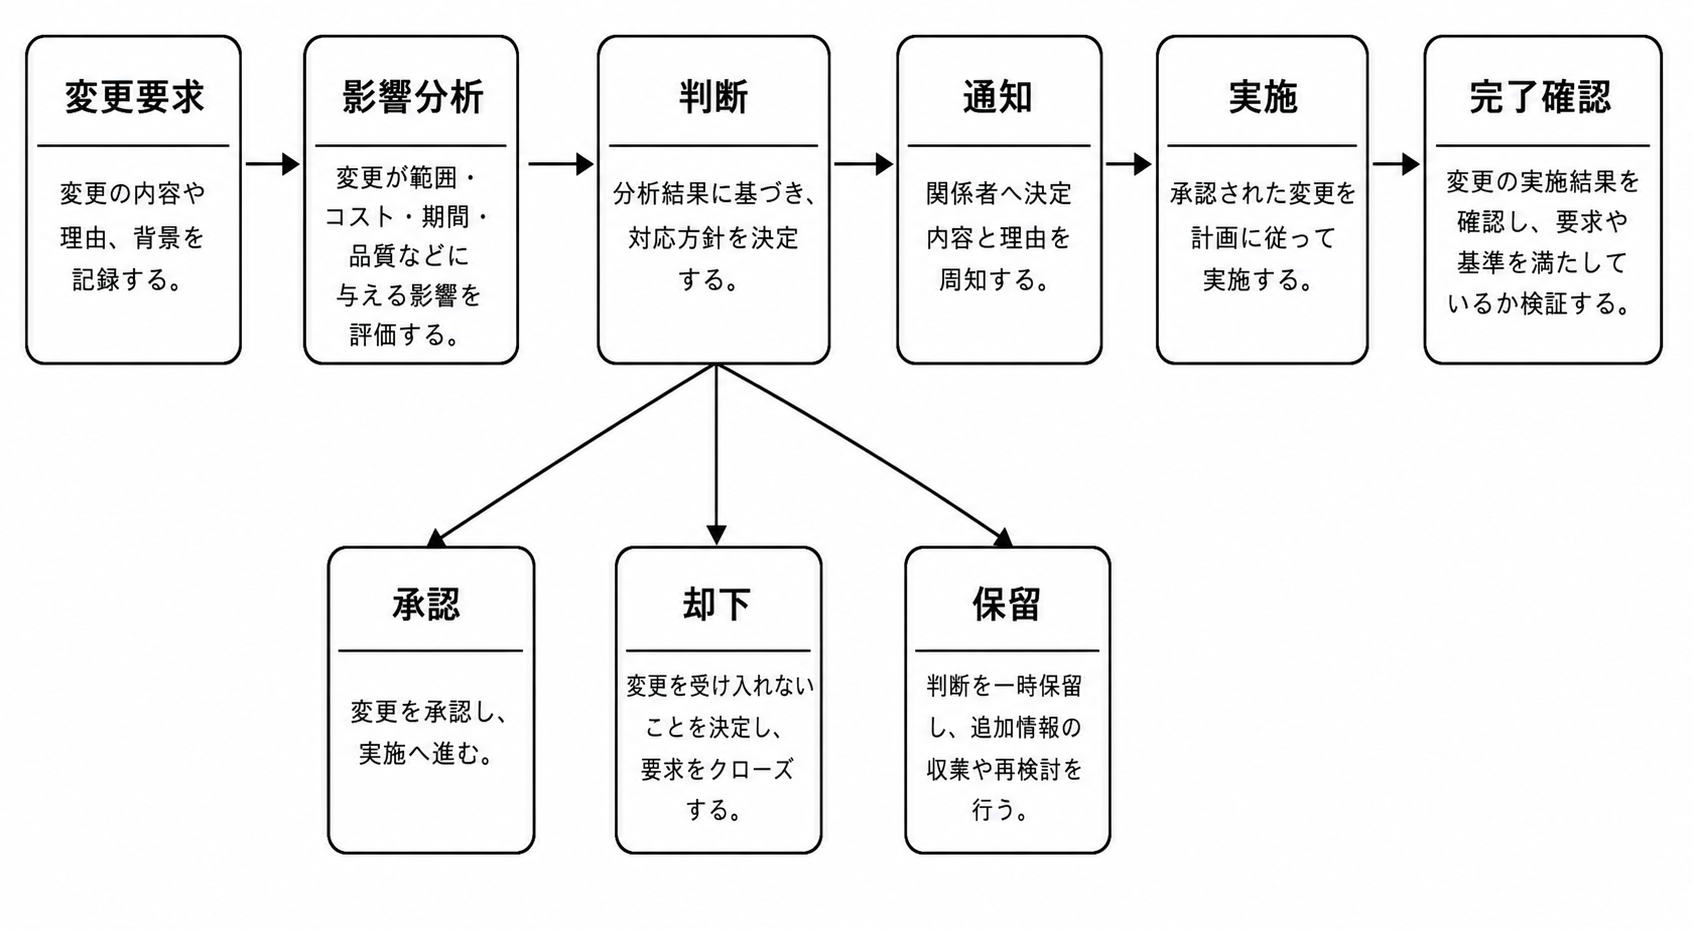
\includegraphics[width=0.96\linewidth]{assets/generated_figures/ch01/fig-ch01-10.png}}{\fbox{\parbox[c][48mm][c]{0.9\linewidth}{\centering 画像生成待ち\\要求変更管理の流れ}}}
\caption{要求変更管理の流れ}
\label{fig:ch01-10}
\end{figure}

\subsection{実務上の考慮}

\subsubsection{要求プロセスの反復性}

現実の要求活動は、一回で終わらない。最初は広く浅く要求を集め、次に重要な部分を深く分析し、その後また不足が見つかって追加で獲得することが多い。要求は幅と深さの両方を持つため、反復的に進めるのが自然である。

ウォーターフォール型では、要求フェーズで多くの要求を先に固める。反復型やアジャイル型では、初期に高レベル要求を押さえ、その後、開発する順に詳細化する。重要なのは、ライフサイクルの名前ではなく、対象ソフトウェアの性質に合う要求活動を選ぶことである。

\subsubsection{要求の優先順位付け}

\term{要求の優先順位付け}は、限られた費用と時間の中で、価値の高い要求から扱うために必要である。優先度は、価値だけでなく、未実現だった場合の不満、実装費用、保守費用、技術リスク、利用されないリスクなどを考慮して決める。

\MiniBox{Kanoモデルの考え方}{ある機能があると満足度が上がる場合と、ないと強い不満が出る場合は異なる。たとえばメールソフトでは、迷惑メールフィルタはあると嬉しい機能かもしれないが、添付ファイルを扱えないと利用者は強く不満を持つ。優先度は満足と不満の両方から考える。}

優先度の表し方には、「必須」「望ましい」「あればよい」のような段階、1から10の数値、優先順位リストなどがある。実務では、細かな数値差よりも、同程度の優先度を持つ要求群を見つけることが重要である。

\subsubsection{要求の追跡可能性}

\term{追跡可能性}とは、要求がどこから来て、どの設計、コード、テスト、文書につながるかをたどれることです。これは二つの目的で役立つ。

第一に、成果物間の整合性確認である。ある要求に対応する設計要素がなければ、その要求は満たされていない可能性がある。逆に、ある設計要素に対応する要求がなければ、その設計要素は不要か、要求が不足している可能性がある。

第二に、変更の影響分析である。ある要求が変わったとき、関連するソフトウェア要求、設計要素、コード、テストケース、利用者文書をたどることで、変更に必要な作業範囲を見積もりやすくなる。

\begin{figure}[htbp]
\centering
\IfFileExists{assets/generated_figures/ch01/fig-ch01-11.png}{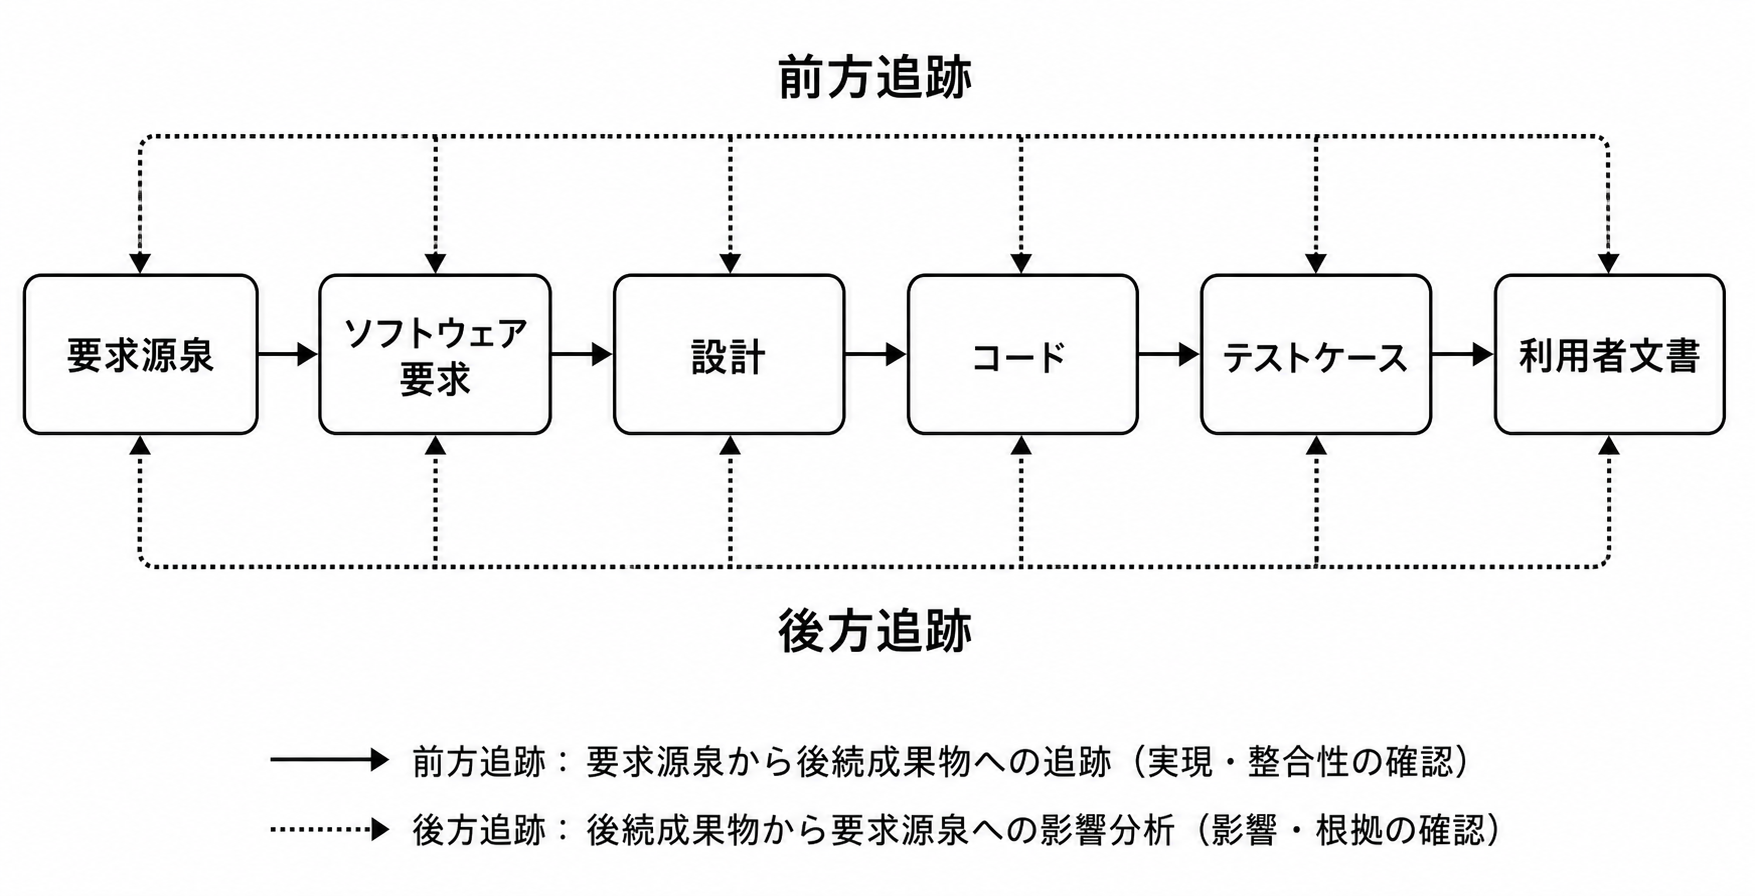
\includegraphics[width=0.96\linewidth]{assets/generated_figures/ch01/fig-ch01-11.png}}{\fbox{\parbox[c][48mm][c]{0.9\linewidth}{\centering 画像生成待ち\\要求追跡の連鎖図}}}
\caption{要求追跡の連鎖図}
\label{fig:ch01-11}
\end{figure}

\subsubsection{要求の安定性と変動性}

\term{要求の安定性}とは、要求が変わりにくい度合いである。\term{変動性}とは、要求が変わりやすい度合いである。

銀行アプリケーションで「口座に利息を計算して付与する」は比較的安定した要求である。一方、税制に基づく特定口座の扱いは、法改正で変わる可能性がある。変わりやすい要求を早く見つけると、変更に強い設計を選びやすくなる。

\subsubsection{要求の測定}

要求を測定する理由は、規模、費用、進捗、品質を管理するためである。\term{機能規模測定}は、機能要求の大きさを測る技法である。アジャイル開発で使われるストーリーポイントも、要求の大きさを表す測度として使われることがある。

要求品質の指標は、曖昧さ、テスト可能性、重複、矛盾、欠落、変更頻度などから作れる。これらを測ることで、要求プロセスの弱点を改善しやすくなる。

\subsubsection{要求プロセスの品質と改善}

要求プロセスの品質は、ソフトウェア製品の費用、納期、顧客満足度に大きく影響する。要求プロセスを改善するには、プロセス改善モデルや品質標準との対応、測定、ベンチマーク、改善計画、実施、振り返りが必要である。

セキュリティの観点では、機密性、完全性、可用性をどのように要求へ反映し、改善するかも重要である。

\subsection{ソフトウェア要求ツール}

要求活動は、紙や表計算ソフトだけでも始められる。しかし、要求が多くなり、変更や追跡が必要になると、専用ツールの支援が重要になる。

\subsubsection{要求管理ツール}

\term{要求管理ツール}は、要求の属性管理、追跡可能性、文書生成、変更管理などを支援する。要求が増えるほど、手作業での追跡は難しくなる。特に、規制対応や安全性が重要な領域では、ツールの価値が高い。

\subsubsection{要求モデリングツール}

\term{要求モデリングツール}は、要求モデルを作成、変更、公開するためのツールである。図を描くだけでなく、構文チェック、整合性確認、完全性確認、シミュレーションなどを支援するものもある。

形式的分析では、定理証明器やモデル検査器のようなツールが使われる。ただし、ツールを使えば自動的にすべてが証明できるわけではなく、形式的な推論に関する知識が必要になる。

\subsubsection{機能テストケース生成ツール}

要求仕様の形式性が高いほど、機能テストケースを機械的に導きやすくなる。たとえば、BDDのシナリオはテストケースへ変換しやすい。状態モデルでは、定義された遷移から正のテストケースを作り、存在しない状態とイベントの組合せから負のテストケースを作れる。

ただし、一般にはツールが入力データを生成できても、期待結果の判断には業務知識が必要になることがある。

\begin{figure}[htbp]
\centering
\IfFileExists{assets/generated_figures/ch01/fig-ch01-12.png}{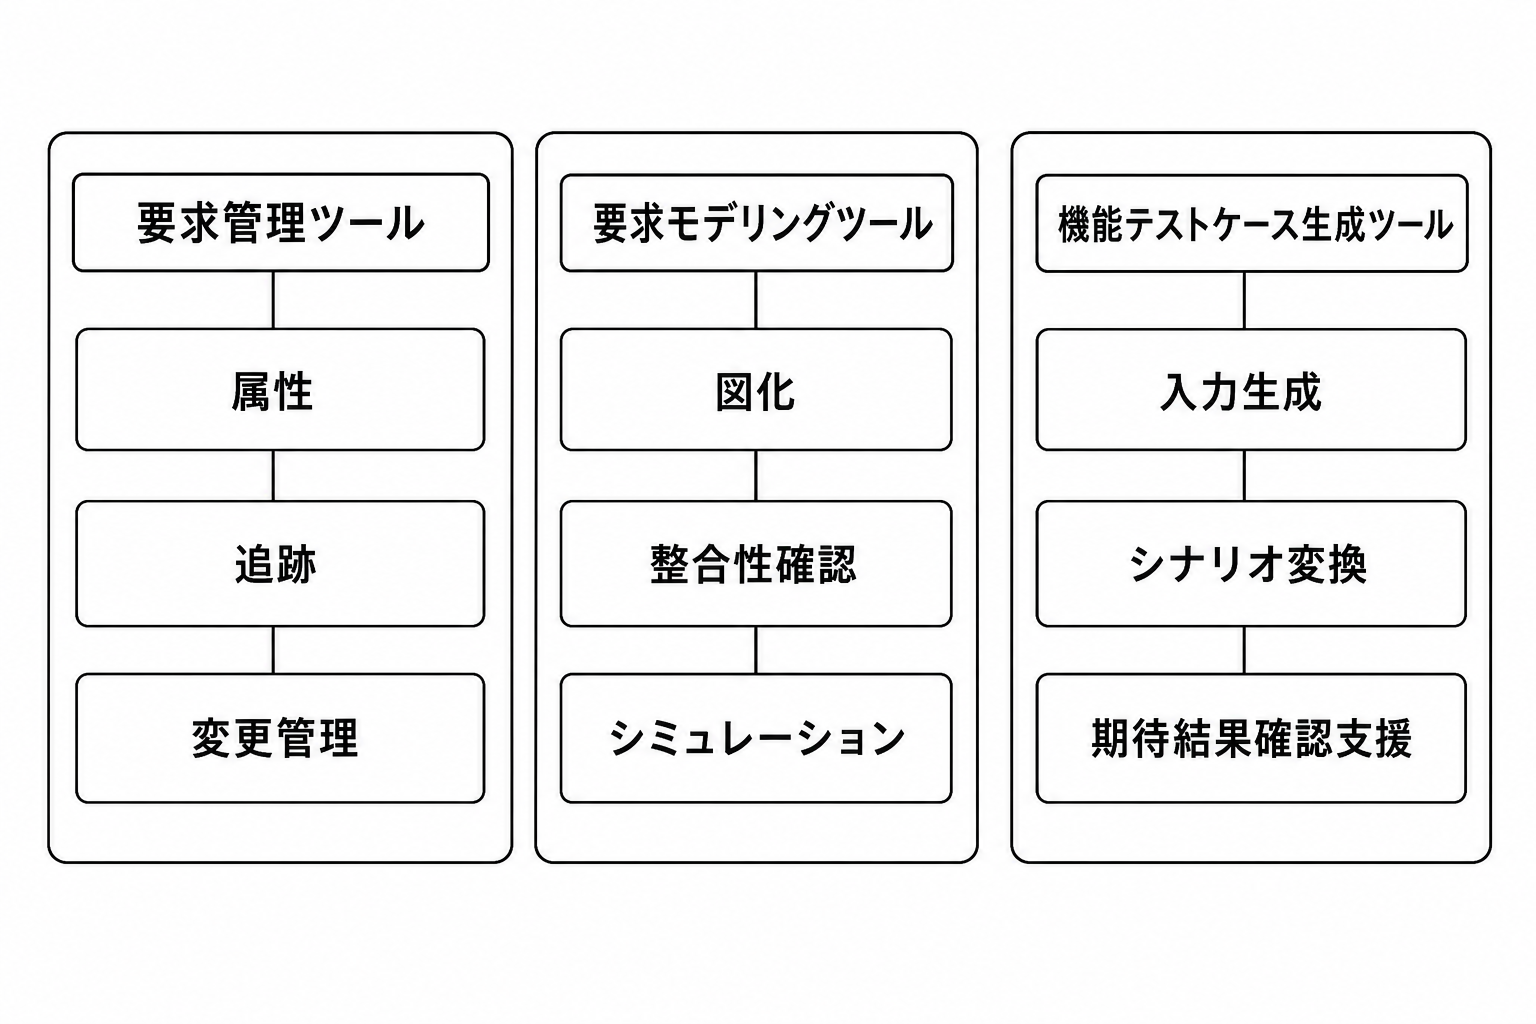
\includegraphics[width=0.96\linewidth]{assets/generated_figures/ch01/fig-ch01-12.png}}{\fbox{\parbox[c][48mm][c]{0.9\linewidth}{\centering 画像生成待ち\\要求ツールの分類図}}}
\caption{要求ツールの分類図}
\label{fig:ch01-12}
\end{figure}

\subsection{トピックと参考文献の対応}

この表は、SWEBOKが示す「トピック対参考資料の行列」を、学習用に簡略化したものである。詳しく学ぶときは、各トピックに対応する文献を読む。

\small
\par\smallskip\noindent\refstepcounter{table}\label{tab:ch01-12}\textbf{表 \thetable: 第01章 ソフトウェア要求 表12}\par\smallskip
\begin{longtable}{@{}p{.38\linewidth}p{.55\linewidth}@{}}
\toprule
トピック & 主な参考資料 \\
\midrule
\endhead
1. ソフトウェア要求の基礎 & Wiegers and Beatty, \textit{Software Requirements}; Sommerville, \textit{Software Engineering} \\
1.1 要求の定義 & Wiegers and Beatty; Sommerville; ISO/IEC/IEEE 24765 \\
1.2 要求分類 & Wiegers and Beatty; Sommerville \\
1.3 製品要求とプロジェクト要求 & Wiegers and Beatty \\
1.4 機能要求 & Wiegers and Beatty; Sommerville \\
1.5 非機能要求 & Wiegers and Beatty; Sommerville; ISO/IEC 25010 \\
1.6 技術制約 & Tockey, \textit{How to Engineer Software}; Yourdon \\
1.7 サービス品質制約 & ISO/IEC 25010; Tockey, \textit{Return on Software} \\
1.8 分類の理由 & Wiegers and Beatty; Tockey; McMenamin and Palmer \\
1.9 システム要求とソフトウェア要求 & INCOSE Handbook; ISO/IEC/IEEE 29148 \\
1.10 派生要求 & Tockey; INCOSE Handbook \\
1.11 要求活動 & Wiegers and Beatty; Sommerville \\
2. 要求獲得 & Wiegers and Beatty; Sommerville; Robertson and Robertson; LaPlante and Kassab \\
2.1 要求源泉 & Wiegers and Beatty; Robertson and Robertson \\
2.2 要求獲得技法 & Wiegers and Beatty; Wood and Silver; Gottesdiener; Brown and Katz \\
3. 要求分析 & Wiegers and Beatty; Sommerville; Tockey \\
3.1 要求の性質 & Wiegers and Beatty; Robertson and Robertson \\
3.2 サービス品質要求の経済性 & Tockey, \textit{Return on Software} \\
3.3 形式的分析 & Sommerville; Wing; Software Engineering Models and Methods \\
3.4 要求衝突への対応 & Robertson and Robertson; Fisher and Ury; Weiss and Lai \\
4. 要求仕様化 & Wiegers and Beatty; Sommerville; ISO/IEC/IEEE 29148 \\
4.1 非構造化自然言語 & Wiegers and Beatty; ISO/IEC/IEEE 29148 \\
4.2 構造化自然言語 & Wiegers and Beatty; Cockburn; Robertson and Robertson \\
4.3 受け入れ基準に基づく仕様化 & Sommerville; Smart; Software Testing KA \\
4.4 モデルに基づく仕様化 & Wiegers and Beatty; Sommerville; Wing; Tockey \\
4.5 要求の追加属性 & Wiegers and Beatty; Gilb \\
4.6 増分的仕様化と包括的仕様化 & Wiegers and Beatty; Robertson and Robertson \\
5. 要求妥当性確認 & Wiegers and Beatty; Sommerville; LaPlante and Kassab \\
5.1 要求レビュー & Wiegers and Beatty; Software Quality KA \\
5.2 シミュレーションと実行 & Tockey; Model-Based Specification references \\
5.3 プロトタイピング & Wiegers and Beatty; Sommerville \\
6. 要求管理活動 & Wiegers and Beatty; Sommerville; McConnell \\
6.1 要求整理・削減 & McConnell, \textit{Rapid Development} \\
6.2 要求変更管理 & Wiegers and Beatty; Sommerville; Software Configuration Management KA \\
6.3 範囲調整 & McConnell; Software Engineering Management KA \\
7. 実務上の考慮 & Wiegers and Beatty; Sommerville; Tockey \\
7.1 反復性 & Sommerville; Robertson and Robertson \\
7.2 優先順位付け & Wiegers and Beatty \\
7.3 追跡可能性 & Wiegers and Beatty; Gotel and Finkelstein \\
7.4 安定性と変動性 & Sommerville; Tockey \\
7.5 要求測定 & Wiegers and Beatty; Software Engineering Process KA \\
7.6 プロセス品質と改善 & Wiegers and Beatty; Software Quality KA \\
8. ソフトウェア要求ツール & Wiegers and Beatty; Sommerville \\
8.1 要求管理ツール & Wiegers and Beatty \\
8.2 要求モデリングツール & Wiegers and Beatty; Sommerville; Formal Methods references \\
8.3 機能テストケース生成ツール & Software Testing KA; Tockey \\
\bottomrule
\end{longtable}
\normalsize

\subsection{発展的な読み物}

SWEBOK第01章で紹介される発展的な読み物を、日本語で読む目的に合わせて整理する。

\par\smallskip\noindent\refstepcounter{table}\label{tab:ch01-13}\textbf{表 \thetable: 第01章 ソフトウェア要求 表13}\par\smallskip
\begin{tabularx}{0.97\linewidth}{@{}p{.31\linewidth}X@{}}
\toprule
文献 & 読むと得られること \\
\midrule
\textit{BABOK Guide} & ビジネス分析全体の知識体系。ソフトウェア要求だけでなく、ビジネス課題、利害関係者、価値の分析を広く学べる。 \\
LaPlante and Kassab & 要求工学を体系的に学ぶための包括的な教科書。 \\
Robertson and Robertson & 要求プロセス、利害関係者、要求発見、要求記述を実務的に学べる。 \\
Gilb & 要求を測定可能にし、価値と品質を重視して記述する考え方を学べる。 \\
Wiegers, \textit{Software Development Pearls} & 長年の実務経験から得られた、要求を含むソフトウェア開発の実践的教訓を学べる。 \\
Fisher and Ury & 要求衝突の解決に役立つ交渉の基本を学べる。 \\
Ahmad & 電子的コミュニケーションを用いた面接で、暗黙知を引き出す方法に関する研究。 \\
\bottomrule
\end{tabularx}

\subsection{参考文献}

\footnotesize
\begin{enumerate}[leftmargin=2.2em,itemsep=.15ex]
\item K. E. Wiegers and J. Beatty, \textit{Software Requirements}, 3rd ed., Microsoft Press, 2013.
\item I. Sommerville, \textit{Software Engineering}, 10th ed., Addison-Wesley, 2016.
\item S. Tockey, \textit{Return on Software: Maximizing the Return on Your Software Investment}, Addison-Wesley, 2005.
\item J. M. Wing, ``A Specifier's Introduction to Formal Methods,'' \textit{Computer}, 1990.
\item P. Laplante and M. Kassab, \textit{Requirements Engineering for Software and Systems}, 4th ed., CRC Press, 2022.
\item S. Robertson and J. Robertson, \textit{Mastering the Requirements Process: Getting Requirements Right}, Addison-Wesley, 2013.
\item T. Gilb, \textit{Competitive Engineering}, Elsevier Butterworth-Heinemann, 2005.
\item E. Yourdon, \textit{Modern Structured Analysis}, Prentice-Hall, 1989.
\item S. Tockey, \textit{How to Engineer Software}, Wiley, 2019.
\item S. Ambler, \textit{Agile Modeling}, Wiley, 2002.
\item A. Cockburn, \textit{Writing Effective Use Cases}, Addison-Wesley, 2000.
\item L. Constantine and L. Lockwood, \textit{Software for Use}, Addison-Wesley, 2000.
\item J. Wood and D. Silver, \textit{Joint Application Development}, Wiley, 1995.
\item E. Gottesdiener, \textit{Requirements by Collaboration}, Addison-Wesley, 2002.
\item J. Terninko, \textit{Step by Step QFD}, 2nd ed., CRC Press, 1997.
\item G. Salvendy, \textit{Handbook of Human Factors}, 4th ed., Wiley, 2012.
\item T. Brown and B. Katz, \textit{Change by Design}, Harper Collins, 2019.
\item S. McMenamin and J. Palmer, \textit{Essential Systems Analysis}, Yourdon Press, 1984.
\item J. Smart, \textit{BDD in Action}, Manning Publications, 2015.
\item D. Weiss and C. Lai, \textit{Software Product-Line Engineering}, Addison-Wesley, 1999.
\item K. Wiegers, \textit{Software Development Pearls}, Addison-Wesley Professional, 2021.
\item S. McConnell, \textit{Rapid Development}, Microsoft Press, 1996.
\item O. Gotel and C. W. Finkelstein, ``An Analysis of the Requirements Traceability Problem,'' 1994.
\item INCOSE, \textit{Systems Engineering Handbook}, International Council on Systems Engineering, 2012.
\item R. Fisher and W. Ury, \textit{Getting to Yes}, 3rd ed., Penguin, 2011.
\item ISO/IEC/IEEE 29148, \textit{Systems and software engineering -- Life cycle processes -- Requirements engineering}, 2018.
\item ISO/IEC 25010, \textit{Systems and software Quality Requirements and Evaluation (SQuaRE) -- System and software quality models}, 2011.
\item ISO/IEC/IEEE 24765:2017, \textit{Systems and Software Engineering -- Vocabulary}, 2nd ed., 2017.
\item N. Ahmad, \textit{Effects of Electronic Communication on the Elicitation of Tacit Knowledge in Interview Techniques for Small Software Developments}, doctoral thesis, University of Huddersfield, 2021.
\item IIBA, \textit{A Guide to the Business Analysis Body of Knowledge (BABOK Guide) v3}, 2015.
\end{enumerate}
\normalsize

\subsection{章末確認問題}

\begin{enumerate}
\item 「利用者は注文番号で注文履歴を検索できる」は、どの分類の要求か。
\item 「検索結果は通常時2秒以内に表示される」は、機能要求か非機能要求か。理由も述べよ。
\item 「実装言語はPythonとする」は、技術制約かサービス品質制約か。
\item 要求獲得と要求分析の違いを、自分の言葉で説明せよ。
\item 要求仕様化において、自然言語、受け入れ基準、モデルの違いを説明せよ。
\item 要求妥当性確認で、レビュー、シミュレーション、プロトタイプはどのように使い分けるか。
\item 要求変更を受け入れるとき、なぜ費用・納期・スコープへの影響を確認する必要があるか。
\item 追跡可能性が、変更時の影響分析に役立つ理由を説明せよ。
\end{enumerate}

\MiniBox{解答の方向性}{1は機能要求。2はサービス品質制約であり非機能要求。3は技術制約。4以降は、本文の「合意を作る活動」「候補要求を表面化させる」「意味・矛盾・実現可能性を調べる」「合意を維持する」といった語を使って説明できる。}

\section{第02章 ソフトウェアアーキテクチャ}
\noindent\textbf{この資料の主張}\par
ソフトウェアアーキテクチャは、単なる「大まかな設計図」ではない。アーキテクチャは、ソフトウェア集約システムにおいて根本的であり、後から変えにくく、多くの品質や費用に影響する構造・関係・原則・重要な意思決定の集合である。よいアーキテクチャは、利害関係者の関心事を整理し、設計・実装・テスト・運用・保守に関わる人々が同じ理解を持つための土台になる。

\begin{statementbox}{この資料の読み方}
専門用語は原則として日本語で示し、必要に応じて英語を括弧内に併記する。英語名は、元資料、規格、ツール、文献で同じ概念を確認するための手がかりとして残す。初学者が前提知識なしに読めるように、各節では「何のための概念か」「実務では何を判断するのか」を重視する。
\end{statementbox}



\subsection*{全体概要：この章で学ぶこと}
\addcontentsline{toc}{subsection}{全体概要：この章で学ぶこと}
この章は、ソフトウェアの根本的な形を決め、関係者が共有し、後工程の判断に使うための「アーキテクチャ」を扱う。ここでいうアーキテクチャは、クラス図や構成図そのものではない。図や文書は、アーキテクチャを表すための手段である。アーキテクチャの中心にあるのは、主要な構成要素、それらの関係、設計と進化の原則、品質特性に関するトレードオフ、そして重要な意思決定である。

\noindent\textbf{到達目標}\quad この章を読み終えると、次のことができるようになる。
\begin{itemize}
  \item 「アーキテクチャ」という語が、分野、活動、成果物の三つの意味で使われることを説明できる。
  \item 利害関係者と関心事を分けて考え、アーキテクチャが誰の何に答えるものかを説明できる。
  \item ビューとビューポイントの違いを説明し、複数の図やモデルを使う理由を説明できる。
  \item アーキテクチャ様式、アーキテクチャパターン、参照アーキテクチャを区別できる。
  \item アーキテクチャ設計を、分析、統合、評価の反復活動として説明できる。
  \item アーキテクチャ評価、レビュー、測度の目的を説明できる。
\end{itemize}

\noindent\textbf{学習順序}\quad 初学者は、まず「アーキテクチャとは何か」と「利害関係者と関心事」を押さえる。その後、「どう記述するか」「どう設計するか」「どう評価するか」という流れで読むとよい。

\begin{figure}[htbp]
\centering
\IfFileExists{assets/generated_figures/ch02/fig-ch02-01.png}{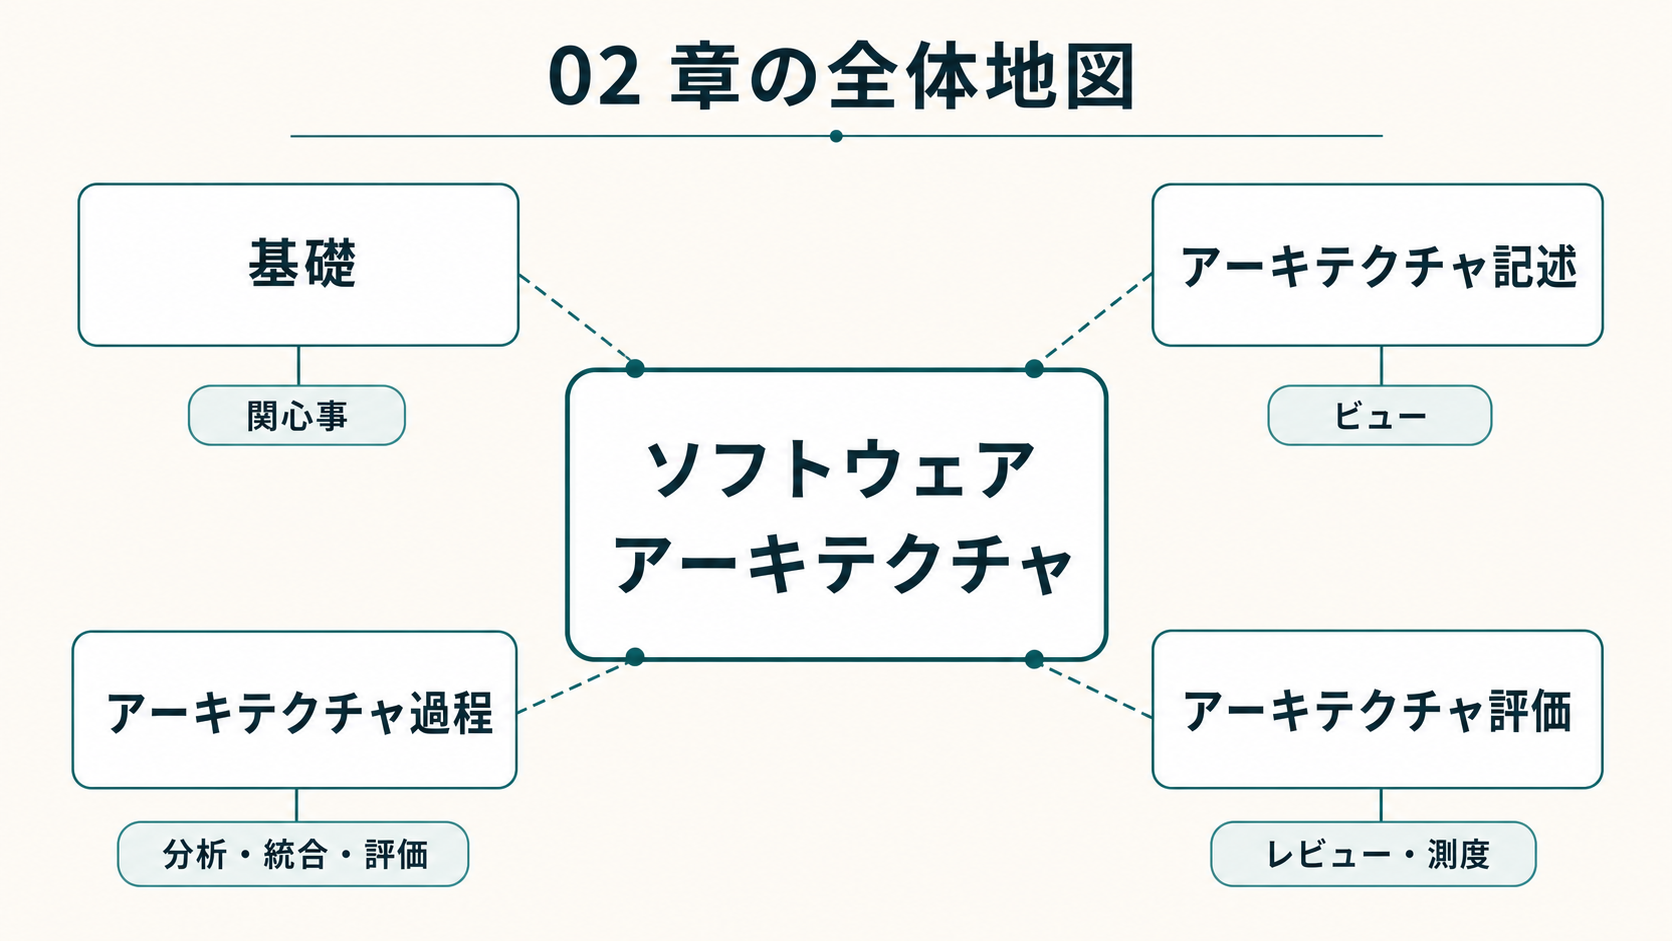
\includegraphics[width=0.96\linewidth]{assets/generated_figures/ch02/fig-ch02-01.png}}{\fbox{\parbox[c][48mm][c]{0.9\linewidth}{\centering 画像生成待ち\\02 章の全体地図}}}
\caption{02 章の全体地図}
\label{fig:ch02-01}
\end{figure}

\subsubsection*{最初に必要な用語}
\addcontentsline{toc}{subsubsection}{最初に必要な用語}
\par\smallskip\noindent\refstepcounter{table}\label{tab:ch02-01}\textbf{表 \thetable: 第02章 ソフトウェアアーキテクチャ 表01}\par\smallskip
\begin{longtable}{P{0.28\linewidth}P{0.64\linewidth}}
\toprule
用語 & 初学者向けの説明 \\
\midrule
ソフトウェア集約システム & ソフトウェアが主要な役割を持つシステムである。ソフトウェアだけでなく、ハードウェア、人、手順、外部サービスも含み得る。 \\
アーキテクチャ & システムの根本的な概念、構成要素、関係、設計と進化の原則である。単なる図ではなく、重要な判断の集合でもある。 \\
利害関係者 & システムに影響を与える、または影響を受ける人や組織である。顧客、利用者、開発者、運用者、保守担当、監査者などが含まれる。 \\
関心事 & 利害関係者が気にする論点である。費用、納期、性能、信頼性、安全性、セキュリティ、使いやすさ、保守しやすさなどである。 \\
品質特性 & システムがどの程度よく振る舞うかを表す性質である。可用性、変更容易性、性能、信頼性、試験容易性などが例である。 \\
アーキテクチャ記述 & アーキテクチャを関係者が使えるように、文書、図、表、モデル、意思決定記録などで表した成果物である。 \\
ビュー & アーキテクチャの一面を表す図やモデルである。論理ビュー、配置ビュー、開発ビューなどがある。 \\
ビューポイント & ビューを作り、読み、使うための規約である。記法、表す要素、関心事、想定読者などを定める。 \\
アーキテクチャ上重要な要求 & アーキテクチャに影響する要求である。英語では Architecturally Significant Requirement、略して ASR と呼ぶ。 \\
アーキテクチャ技術的負債 & 今のアーキテクチャ判断が、将来の変更・運用・保守に追加費用を生む状態である。 \\
\bottomrule
\end{longtable}

\subsection*{導入：なぜソフトウェアアーキテクチャを独立して学ぶのか}
\addcontentsline{toc}{subsection}{導入：なぜソフトウェアアーキテクチャを独立して学ぶのか}
SWEBOK v4.0a では、ソフトウェアアーキテクチャをソフトウェア設計から独立した知識領域として扱う。これは、1990 年代以降にアーキテクチャ研究と実務が大きく発展し、設計の一部としてだけでは説明しきれない知識が増えたためである。

ソフトウェアアーキテクチャは、概念、表現、作業成果物、文脈、過程、方法、分析、評価という複数の視点から理解する必要がある。特に大規模なシステムでは、個々の実装詳細よりも先に、主要な構成要素、構成要素間の関係、外部環境との相互作用、品質特性への対応、変更に対する耐性を考える必要がある。

\begin{statementbox}{重要}
アーキテクチャは「実装の前に一度だけ描く図」ではない。要求、品質、組織、運用、保守、将来の進化に関わる継続的な判断の集合である。
\end{statementbox}

\subsection{ソフトウェアアーキテクチャの基礎}

\subsubsection{「アーキテクチャ」という語の意味}
ソフトウェア工学では、「アーキテクチャ」という語が少なくとも三つの意味で使われる。

第一に、アーキテクチャは\keyterm{分野}を指す。これは、ソフトウェア集約システムを構成するための考え方、原則、過程、方法を扱う知識領域である。建築における建築学が、建物をどう構成するかを扱うのと同じように、ソフトウェアアーキテクチャは、ソフトウェア集約システムをどう構成するかを扱う。

第二に、アーキテクチャは\keyterm{活動}を指す。アーキテクチャを作る活動は、しばしば「アーキテクチャ設計」または「アーキテクティング」と呼ばれる。ソフトウェア設計は、一般にアーキテクチャ設計、高水準設計、詳細設計に分けられる。この章は、その中でも根本的な構造や重要な意思決定に関わる部分を扱う。

第三に、アーキテクチャは\keyterm{成果}を指す。つまり、あるシステムについて、主要な構成要素、関係、原則、設計判断がどのようになっているかという結果である。この成果は、アーキテクチャ記述として表される。

かつての定義では、アーキテクチャは「システムまたは構成要素の組織構造」と理解されることが多かった。しかし、現代の考え方では、単なる構造だけでは足りない。ソフトウェアには、コード構造だけでなく、実行時構造、配置構造、情報構造、開発組織との対応、運用構造など、複数の構造がある。また、アーキテクチャは環境の中のシステムとして考える必要がある。

\begin{definitionbox}
ソフトウェアアーキテクチャとは、システムの環境における根本的な概念または性質であり、構成要素、構成要素間の関係、設計と進化の原則として表れるものである。
\end{definitionbox}

この定義の要点は二つである。第一に、アーキテクチャはすべての詳細を含むものではなく、根本的なものを扱う。第二に、アーキテクチャはシステムの外側も見る。利用者、組織、外部システム、ハードウェア、法律、規制、運用環境などとの関係が重要である。

\begin{figure}[htbp]
\centering
\IfFileExists{assets/generated_figures/ch02/fig-ch02-02.png}{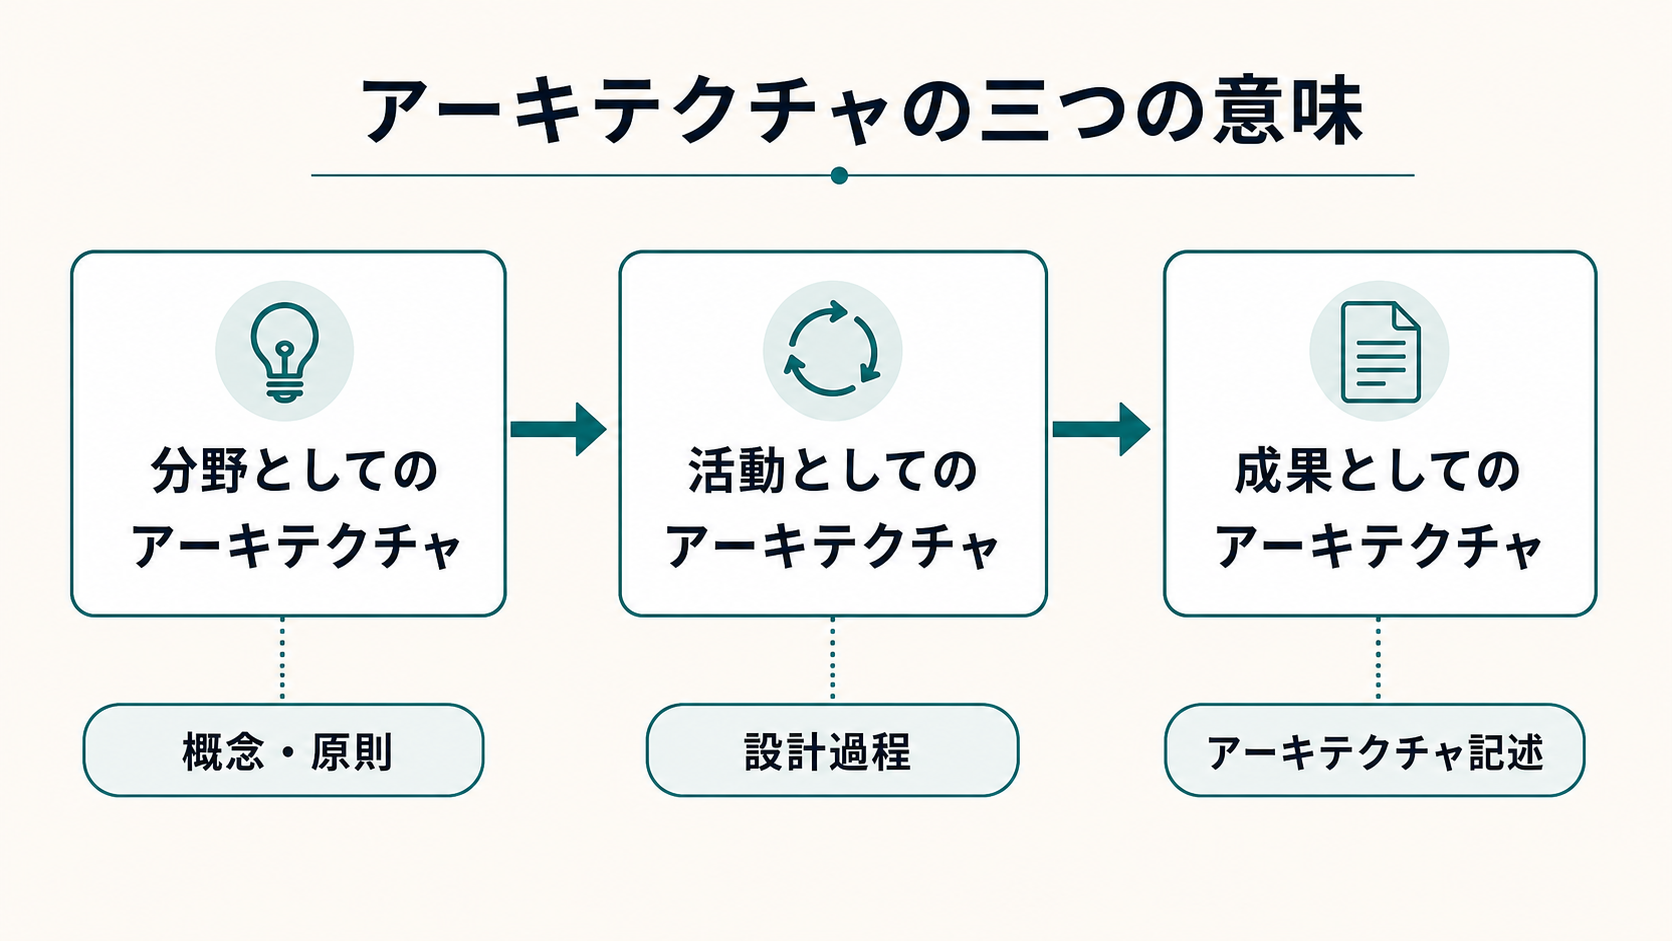
\includegraphics[width=0.96\linewidth]{assets/generated_figures/ch02/fig-ch02-02.png}}{\fbox{\parbox[c][48mm][c]{0.9\linewidth}{\centering 画像生成待ち\\アーキテクチャの三つの意味}}}
\caption{アーキテクチャの三つの意味}
\label{fig:ch02-02}
\end{figure}

\subsubsection{利害関係者と関心事}
ソフトウェアシステムには、多くの利害関係者がいる。顧客は、いつ完成するか、いくらかかるか、投資に見合う価値があるかを気にする。利用者は、何ができるか、使いやすいか、作業を妨げないかを気にする。開発者は、構成要素の責任、インタフェース、依存関係、実装しやすさを気にする。運用担当は、配置、監視、障害対応、復旧、性能を気にする。保守担当は、変更しやすさ、影響範囲のわかりやすさ、技術的負債を気にする。

このような「気にする論点」を\keyterm{関心事}\en{concern}という。アーキテクチャの重要な役割は、利害関係者ごとの関心事を整理し、それぞれに答えられる表現を用意することである。

\begin{statementbox}{関心事の分離}
複雑なシステムを一度にすべて理解しようとすると、論点が混ざる。関心事の分離とは、性能、安全性、セキュリティ、使いやすさ、保守性などを、必要に応じて分けて考える方法である。分けることは、他の関心事を無視することではなく、順序立てて考えるための技法である。
\end{statementbox}

関心事は、機能的なもの、非機能的なもの、制約の形を取るものに分けられる。さらに、技術、事業、運用、組織、政治、経済、法令、規制、環境、社会的影響など、非常に広い範囲にまたがる。近年は、気候変動への意識の高まりにより、エネルギー効率や持続可能性もアーキテクチャ上の関心事になっている。

\par\smallskip\noindent\refstepcounter{table}\label{tab:ch02-02}\textbf{表 \thetable: 第02章 ソフトウェアアーキテクチャ 表02}\par\smallskip
\begin{longtable}{P{0.25\linewidth}P{0.67\linewidth}}
\toprule
利害関係者 & 典型的な関心事 \\
\midrule
顧客・発注者 & 費用、納期、事業価値、契約適合性、長期的な運用費である。 \\
利用者 & 機能、使いやすさ、応答時間、信頼性、利用体験である。 \\
開発者 & 構成要素の責任、インタフェース、依存関係、実装容易性、テスト容易性である。 \\
運用担当 & 配置、監視、可用性、障害復旧、容量、セキュリティ運用である。 \\
保守担当 & 変更容易性、理解しやすさ、技術的負債、互換性である。 \\
監査・認証担当 & 法令・規格への適合、証拠、説明可能性、安全性、セキュリティである。 \\
\bottomrule
\end{longtable}

\begin{figure}[htbp]
\centering
\IfFileExists{assets/generated_figures/ch02/fig-ch02-03.png}{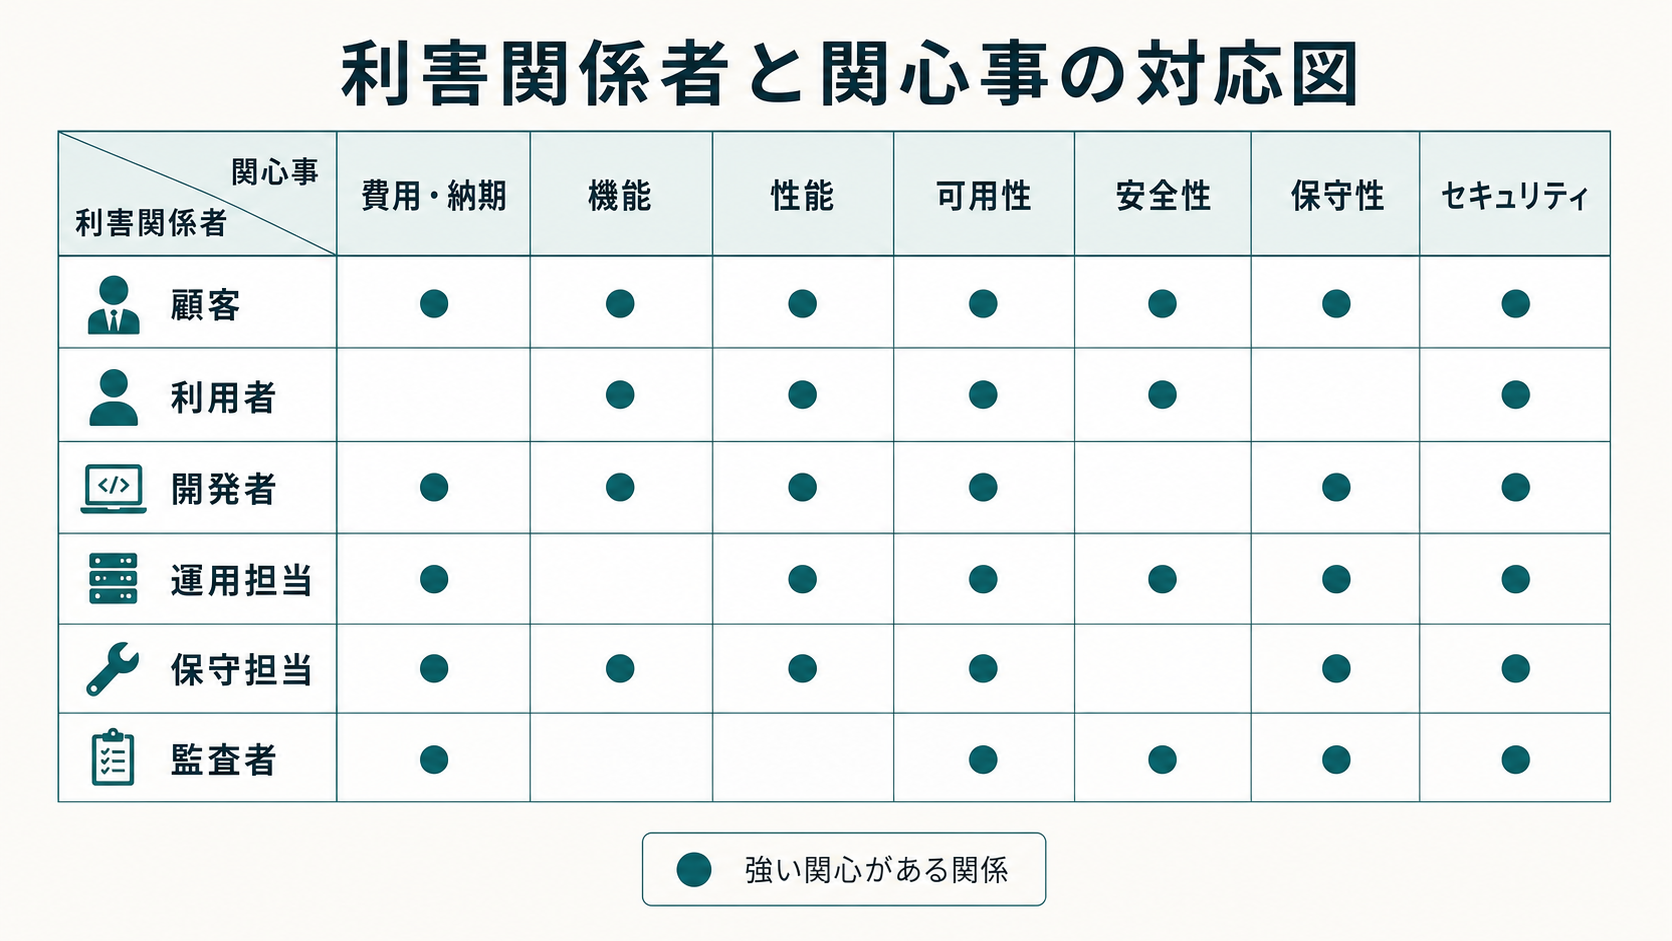
\includegraphics[width=0.96\linewidth]{assets/generated_figures/ch02/fig-ch02-03.png}}{\fbox{\parbox[c][48mm][c]{0.9\linewidth}{\centering 画像生成待ち\\利害関係者と関心事の対応図}}}
\caption{利害関係者と関心事の対応図}
\label{fig:ch02-03}
\end{figure}

\subsubsection{アーキテクチャの用途}
アーキテクチャの第一の用途は、システムに関わる人々が共有理解を持つことである。共有理解がなければ、設計者、開発者、テスト担当、運用担当が異なる前提で作業し、結果として整合しないシステムになりやすい。

第二の用途は、設計と構築の指針を与えることである。アーキテクチャは、どの構成要素が存在するか、どの構成要素がどの責任を持つか、どのように通信するか、どの品質特性をどの方法で満たすかを示す。これにより、実装前に代替案を比較し、リスクを見つけられる。

第三の用途は、既存システムの理解である。保守、拡張、移行、改善を行うとき、既存システムのアーキテクチャを理解することが重要である。これは、逆方向の設計理解、すなわちリバースアーキテクティングに近い活動である。

また、アーキテクチャは組織構造とも関係する。コンウェイの法則は、システムの構造が、それを設計する組織のコミュニケーション構造を反映しやすいことを指摘する。組織とアーキテクチャの対応は、うまく使えば分担と責任を明確にする力になるが、悪く働くと不要な分断や複雑な依存関係を生む。

\begin{statementbox}{実務での見方}
アーキテクチャは、計画、見積り、分担、再利用、製品系列化にも使われる。単一システムの内部構造だけでなく、複数製品に共通する土台を作るためにも重要である。
\end{statementbox}

\subsection{ソフトウェアアーキテクチャ記述}

\subsubsection*{アーキテクチャ記述の役割}
\addcontentsline{toc}{subsubsection}{アーキテクチャ記述の役割}
小さなシステムを一人で作る場合、アーキテクチャは頭の中にあるだけでも作業できることがある。しかし、大規模で複雑なシステムをチームで作り、運用し、保守する場合には、頭の中の理解だけでは不十分である。人が入れ替わり、要求が変わり、構成が進化するため、アーキテクチャを具体的な成果物として残す必要がある。

この成果物を\keyterm{アーキテクチャ記述}\en{architecture description}という。アーキテクチャ記述は、開発者にとっては構築の設計図であり、テスト担当、品質保証担当、認証担当、運用担当、保守担当にとっては、自分の作業を進めるための根拠である。

かつては、アーキテクチャ記述は文章と非形式的な図で行われることが多かった。しかし、利害関係者と関心事が多様になるにつれて、単一の図ですべてを表すことは難しくなった。そのため、目的や読者に応じて複数のビューを使う方法が重要になった。

\subsubsection{アーキテクチャビューとビューポイント}
\keyterm{ビュー}\en{architecture view}とは、アーキテクチャの一面を表すものである。たとえば、機能要求をどう満たすかを示す論理ビュー、並行処理や実行時相互作用を示すプロセスビュー、システムをどこに配置するかを示す物理ビュー、実装単位や依存関係を示す開発ビューがある。

ビューを分ける理由は、関心事を分離するためである。性能を確認したい人、安全性を確認したい人、配置を考える人、コード分担を考える人は、それぞれ必要な情報が違う。一つの図にすべてを詰め込むと、誰にとっても読みにくい図になる。

\keyterm{ビューポイント}\en{architecture viewpoint}とは、ビューを作成し、解釈し、利用するための規約である。どの要素を使うか、どの関係を描くか、どの記法を使うか、どの関心事に答えるか、誰が読むかを定める。ビューポイントは、ビューの「描き方の型」である。

\par\smallskip\noindent\refstepcounter{table}\label{tab:ch02-03}\textbf{表 \thetable: 第02章 ソフトウェアアーキテクチャ 表03}\par\smallskip
\begin{longtable}{P{0.25\linewidth}P{0.67\linewidth}}
\toprule
種類 & 説明 \\
\midrule
モジュールビューポイント & 実装単位としてのモジュール、その責任、依存関係、分割を表す。 \\
構成要素・接続子ビューポイント & 実行時の大きな構成要素と、それらをつなぐ通信・接続関係を表す。 \\
論理ビューポイント & 対象領域の主要概念、能力、関係を表す。 \\
シナリオ・ユースケースビューポイント & 利用者がシステムとどのように相互作用するかを表す。 \\
情報ビューポイント & 重要な情報、データの保管、アクセス、流れを表す。 \\
配置ビューポイント & ソフトウェアをどの実行環境、機器、ネットワークに置くかを表す。 \\
\bottomrule
\end{longtable}

複数のビューを使うと、別の問題が生じる。ビュー同士が矛盾する可能性である。たとえば、開発ビューでは存在する構成要素が配置ビューにはない、または論理ビューの関係が実行時ビューで説明されていない、といった問題である。これを複数ビュー問題という。対策として、ビュー間の対応関係、追跡可能性、整合性規則を明示する必要がある。

ビューを構成する方法には二つの代表的な考え方がある。\keyterm{合成的手法}では、複数のビューを別々に作り、対応規則で統合する。\keyterm{射影的手法}では、一つの統一モデルから複数のビューを取り出す。射影的手法は整合性を保ちやすいが、統一モデルが表せない関心事には弱い。

\begin{figure}[htbp]
\centering
\IfFileExists{assets/generated_figures/ch02/fig-ch02-04.png}{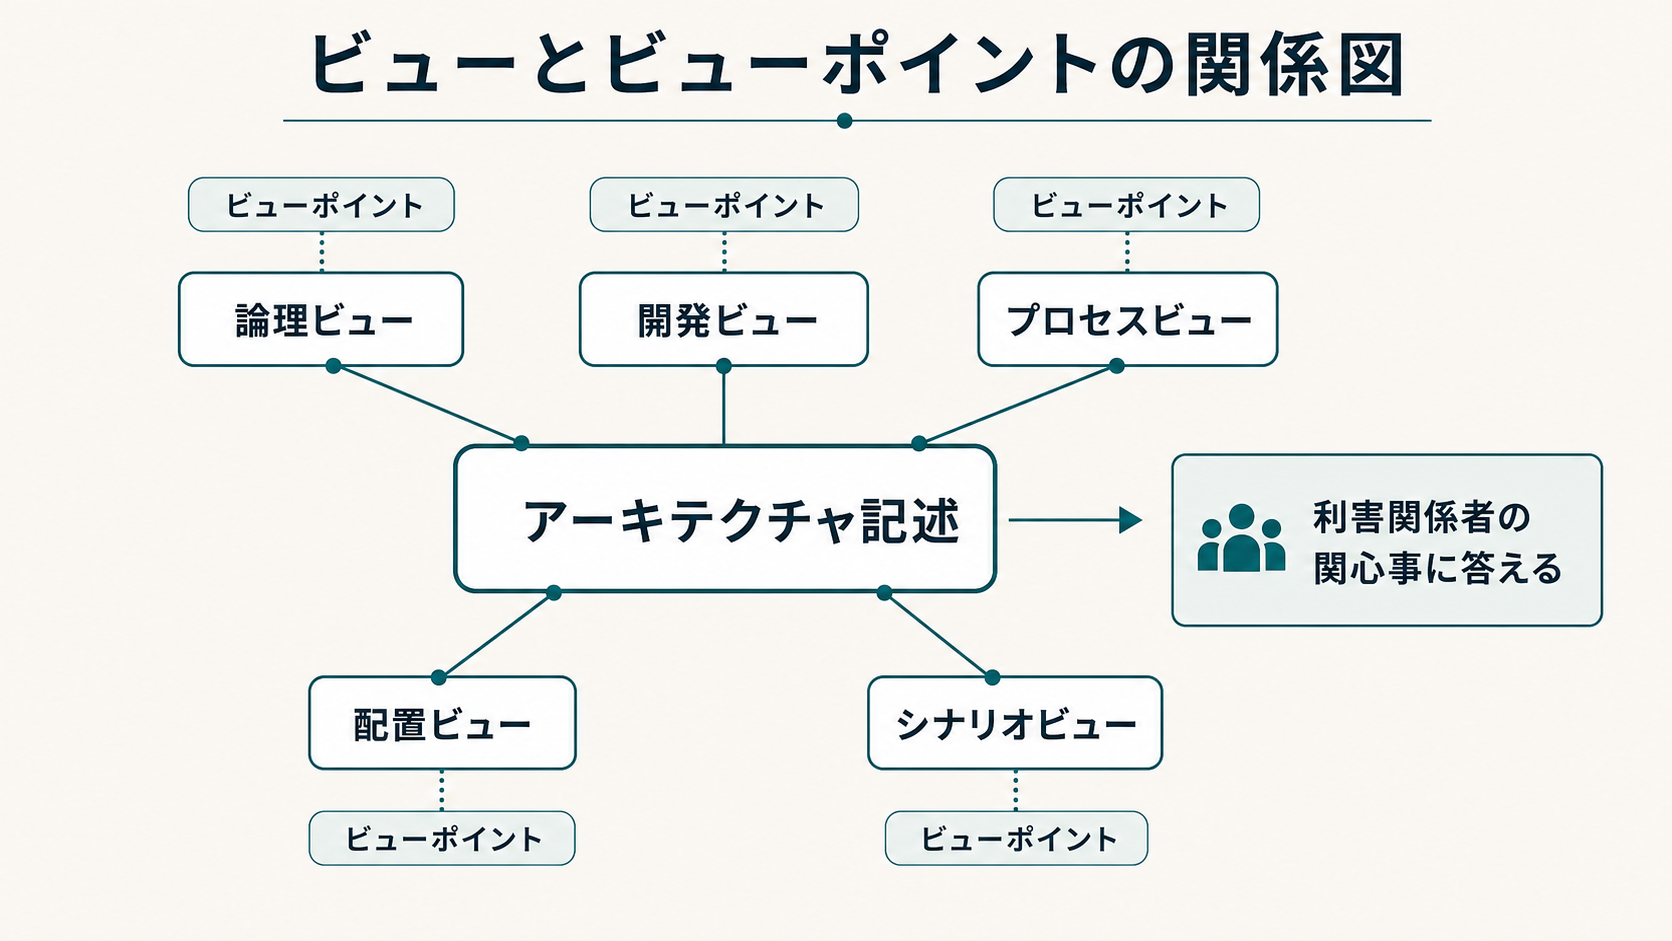
\includegraphics[width=0.96\linewidth]{assets/generated_figures/ch02/fig-ch02-04.png}}{\fbox{\parbox[c][48mm][c]{0.9\linewidth}{\centering 画像生成待ち\\ビューとビューポイントの関係図}}}
\caption{ビューとビューポイントの関係図}
\label{fig:ch02-04}
\end{figure}

\subsubsection{アーキテクチャパターン、様式、参照アーキテクチャ}
\keyterm{アーキテクチャ様式}\en{architectural style}とは、ソフトウェアシステムを構成する特定の作り方であり、システム全体または大きな部分に特徴を与える。たとえば、層化様式、パイプ・アンド・フィルタ、クライアントサーバ、n 層構成、マイクロサービスなどがある。

\keyterm{アーキテクチャパターン}\en{architectural pattern}とは、ソフトウェアシステムの文脈で繰り返し現れる問題に対する共通の解決法である。様式がシステム全体の大きな構成傾向を表しやすいのに対し、パターンは特定の問題への再利用可能な解決法として理解しやすい。ただし、両者の境界は厳密ではない。様式をパターンとして表すこともある。

\par\smallskip\noindent\refstepcounter{table}\label{tab:ch02-04}\textbf{表 \thetable: 第02章 ソフトウェアアーキテクチャ 表04}\par\smallskip
\begin{longtable}{P{0.28\linewidth}P{0.30\linewidth}P{0.30\linewidth}}
\toprule
分類 & 例 & 初学者向けの理解 \\
\midrule
一般的な構造 & 層化、呼出し復帰、パイプ・アンド・フィルタ、黒板、サービス、マイクロサービス & 大きな構成の型である。 \\
分散システム & クライアントサーバ、n 層、ブローカ、発行購読、REST & ネットワーク越しの構成や通信の型である。 \\
方法に基づく構造 & オブジェクト指向、イベント駆動、データフロー & 設計や処理の考え方に基づく型である。 \\
利用者相互作用 & モデル・ビュー・コントローラ、表示・抽象・制御 & 画面や操作の分離に関する型である。 \\
適応システム & マイクロカーネル、反射、メタレベルアーキテクチャ & 変化や拡張に対応しやすくする型である。 \\
\bottomrule
\end{longtable}

\keyterm{参照アーキテクチャ}\en{reference architecture}とは、他のアーキテクチャを導く、または制約するアーキテクチャである。個別システム、製品系列、特定領域のシステムを作るときの共通基盤になる。自動車、医療、モノのインターネット、クラウド、航空電子、製造、通信などの領域で使われる。

\begin{statementbox}{区別の目安}
様式は「全体としてどのような形で作るか」、パターンは「繰り返す問題にどう答えるか」、参照アーキテクチャは「ある領域で個別アーキテクチャを作るための基準」である。
\end{statementbox}

\begin{figure}[htbp]
\centering
\IfFileExists{assets/generated_figures/ch02/fig-ch02-05.png}{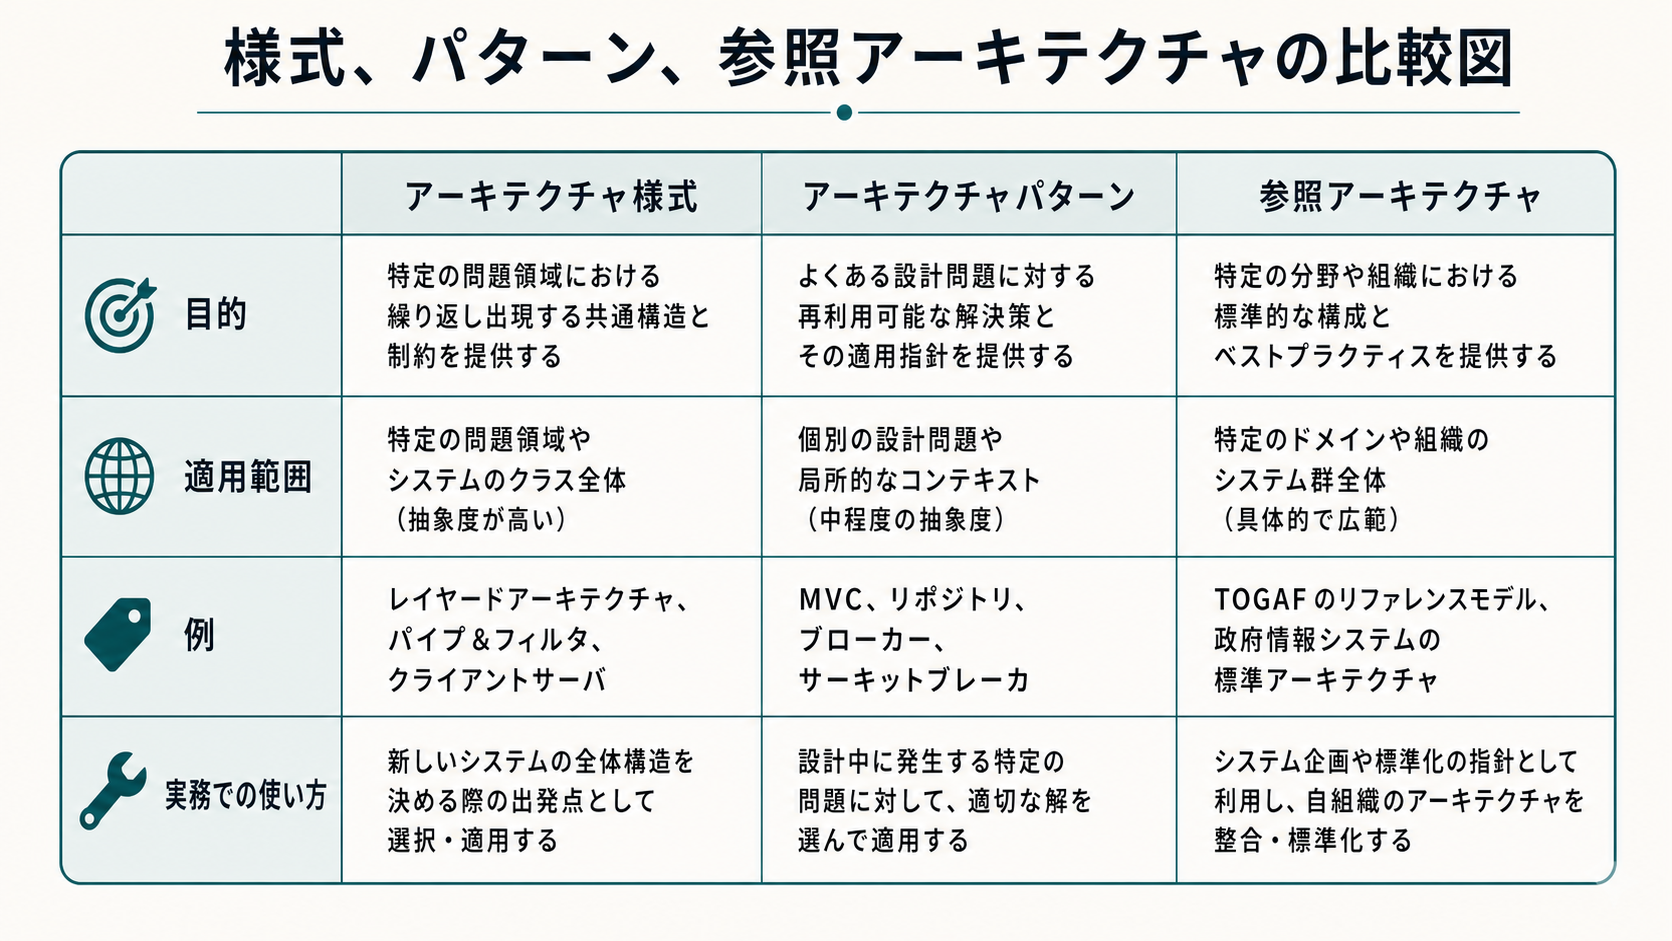
\includegraphics[width=0.96\linewidth]{assets/generated_figures/ch02/fig-ch02-05.png}}{\fbox{\parbox[c][48mm][c]{0.9\linewidth}{\centering 画像生成待ち\\様式、パターン、参照アーキテクチャの比較図}}}
\caption{様式、パターン、参照アーキテクチャの比較図}
\label{fig:ch02-05}
\end{figure}

\subsubsection{アーキテクチャ記述言語とアーキテクチャ枠組み}
\keyterm{アーキテクチャ記述言語}\en{Architecture Description Language, ADL}とは、ソフトウェアアーキテクチャを表すための領域特化言語である。ADL は、もともと大規模プログラミングにおけるモジュール相互接続言語から発展した。特定の領域や様式を対象にするものもあれば、企業全体の関心事を扱う広いものもある。

UML はソフトウェア設計で広く使われるため、アーキテクチャ記述にも使われることが多い。ADL の価値は、単に図を描くことだけではない。アーキテクチャ分析、整合性確認、場合によってはコード生成を支援できる点にある。

\keyterm{アーキテクチャ枠組み}\en{architecture framework}とは、特定領域や利害関係者共同体の中で、アーキテクチャを記述するための規約、原則、実践をまとめたものである。複数のビューポイントや ADL を組み合わせ、推奨される作業方法を定める。自動車分野の AUTOSAR、統一アーキテクチャ枠組み、オープン分散処理の参照モデルなどが例である。

\begin{statementbox}{実務での使い分け}
小規模なシステムでは、軽量な図と意思決定記録で十分なことがある。一方、複数組織、規制領域、製品系列、長期運用システムでは、ADL や枠組みを使うことで整合性と説明可能性を高められる。
\end{statementbox}

\subsubsection{重要な意思決定としてのアーキテクチャ}
アーキテクチャ設計は創造的な活動である。アーキテクトは、要求、品質特性、制約、利用可能な資源、組織の状況を踏まえ、多くの意思決定を行う。特に、品質特性のトレードオフは重要である。性能を高める選択が保守性を下げることがあり、セキュリティを高める選択が使いやすさや費用に影響することがある。

アーキテクチャは、意思決定の網として理解できる。ある決定が、次の決定の前提になる。したがって、重要な判断は、理由とともに記録する必要がある。

\begin{statementbox}{アーキテクチャ根拠}
アーキテクチャ根拠とは、なぜその決定をしたのかを説明する情報である。前提、検討した代替案、選択基準、トレードオフ、却下した案とその理由を含む。将来の保守担当者にとって、決定の理由は決定内容と同じくらい重要である。
\end{statementbox}

\keyterm{アーキテクチャ技術的負債}とは、現在のアーキテクチャ判断が将来の変更や運用に余分な費用を生む状態である。たとえば、初回リリースのためにモジュール性を十分考えずに作ると、後続リリースで機能追加のたびに大きな改修が必要になり、欠陥も増えやすい。この負債は、最初に判断した人ではなく、後から開発や保守を行う人が支払うことが多い。

\begin{figure}[htbp]
\centering
\IfFileExists{assets/generated_figures/ch02/fig-ch02-06.png}{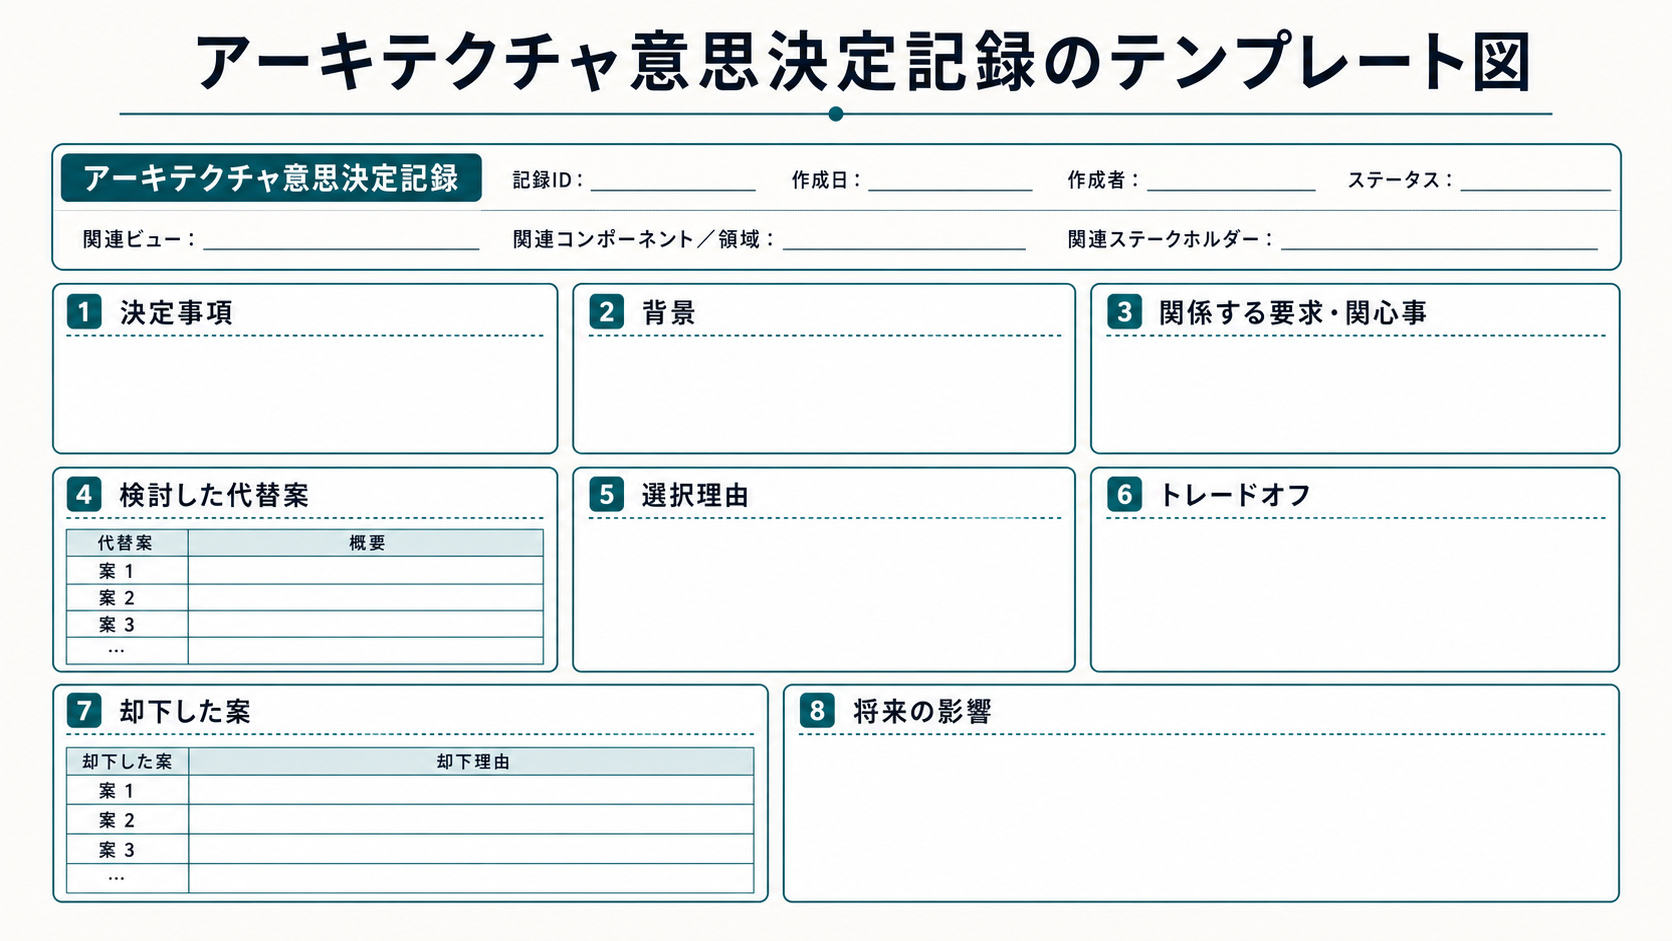
\includegraphics[width=0.96\linewidth]{assets/generated_figures/ch02/fig-ch02-06.png}}{\fbox{\parbox[c][48mm][c]{0.9\linewidth}{\centering 画像生成待ち\\アーキテクチャ意思決定記録のテンプレート図}}}
\caption{アーキテクチャ意思決定記録のテンプレート図}
\label{fig:ch02-06}
\end{figure}

\subsection{ソフトウェアアーキテクチャ過程}

\subsubsection*{アーキテクチャ過程の全体像}
\addcontentsline{toc}{subsubsection}{アーキテクチャ過程の全体像}
アーキテクチャ設計は、単純な一方向の工程ではない。一般的には、関心事と要求を理解する分析、候補解を作る統合、候補解を検証する評価を反復する。要求が変わり、制約が明らかになり、評価で問題が見つかるたびに、分析と統合に戻る。

\subsubsection{文脈の中のアーキテクチャ}
アーキテクチャは真空中で作られるものではない。どの開発ライフサイクルを使うか、製品系列の中にあるか、企業全体のアーキテクチャに従うか、システム・オブ・システムズの一部かによって、作り方が変わる。

伝統的なライフサイクルでは、要求に基づいてアーキテクチャ設計段階を置くことが多い。このとき、すべての要求が同じ重要度を持つわけではない。アーキテクチャに強く影響する要求、すなわち ASR を見極める必要がある。

製品系列や製品ファミリでは、共通のアーキテクチャが先に作られ、それを土台として個別製品が作られる。個別製品は、共通部分と可変部分を持つ。共通アーキテクチャは再利用性を高めるが、過度に固定すると個別製品の自由度を下げる。

アジャイル開発では、明示的なアーキテクチャ設計段階が小さいことがあり、コードからアーキテクチャが「創発する」と説明されることもある。この考え方は、利用者中心の情報システムではうまく働く場合がある。しかし、組込みシステム、サイバーフィジカルシステム、安全性が重要なシステムでは、利用者物語に現れにくい重要品質があるため、意識的なアーキテクチャ検討が必要である。

企業アーキテクチャやシステム・オブ・システムズの文脈では、上位のアーキテクチャが個別ソフトウェアの要求や制約になる。仕様、API、準拠試験、標準インタフェースなどを通じて制約が課される。

\paragraph{アーキテクチャと設計の関係}
アーキテクチャと設計の境界は、しばしば曖昧である。アーキテクチャはソフトウェア設計から発展してきた分野であり、設計の一部として扱われることもある。しかし、実務上は区別して考えると理解しやすい。

\par\smallskip\noindent\refstepcounter{table}\label{tab:ch02-05}\textbf{表 \thetable: 第02章 ソフトウェアアーキテクチャ 表05}\par\smallskip
\begin{longtable}{P{0.22\linewidth}P{0.38\linewidth}P{0.32\linewidth}}
\toprule
観点 & アーキテクチャ & 設計 \\
\midrule
扱う範囲 & システム全体、環境、主要構成、品質特性、進化原則である。 & 構成要素の詳細、データ構造、アルゴリズム、実装方法である。 \\
要求との関係 & 要求を受けるだけでなく、利害関係者との交渉を通じて要求を形作ることがある。 & 既に定義された要求とアーキテクチャ制約を満たす方法を具体化する。 \\
変更影響 & 後から変更すると広範囲に影響しやすい。 & 比較的局所的に変更できる場合が多い。 \\
主な成果物 & アーキテクチャ記述、ビュー、意思決定記録、原則である。 & 詳細設計、インタフェース仕様、クラス設計、アルゴリズム設計である。 \\
\bottomrule
\end{longtable}

\begin{statementbox}{見分け方}
「この判断を後から変えると、多くの構成要素、品質特性、組織分担、運用方法に影響するか」と問う。影響が広ければ、アーキテクチャ判断である可能性が高い。
\end{statementbox}

\subsubsection{アーキテクチャ設計}
アーキテクチャ設計とは、設計原則と方法を使い、ソフトウェアアーキテクチャを作成し、記録する活動である。ここでは、システムの主要構成要素、その責任、性質、インタフェース、相互作用、環境との関係を決める。

典型的な関心事には、次のものがある。
\begin{itemize}
  \item 全体のアーキテクチャ様式と計算パラダイムである。
  \item システムを主要構成要素へ分割する方法である。
  \item 構成要素間の通信、同期、データ交換、制御の流れである。
  \item 関心事と設計責任をどの構成要素に割り当てるかである。
  \item 構成要素のインタフェースである。
  \item 性能、拡張性、資源消費、信頼性への対応である。
  \item 安全性やセキュリティのような全体横断的関心事への対応である。
\end{itemize}

アーキテクチャ設計は、\keyterm{分析}、\keyterm{統合}、\keyterm{評価}の三つの活動を反復する。

\paragraph{アーキテクチャ分析}
アーキテクチャ分析は、アーキテクチャ上重要な要求、すなわち ASR を集め、整理する活動である。ASR は、アーキテクチャに影響する要求である。たとえば、厳しい応答時間、大量アクセスへの拡張性、高い可用性、法規制への適合、強いセキュリティ、外部システムとの接続方式などが該当する。

分析では、既知の要求、利害関係者のニーズ、環境制約、上位アーキテクチャ、利用可能な資源を確認する。要求と制約の組合せが実現困難な場合には、利害関係者と交渉し、期待や要求を調整する必要がある。

\paragraph{アーキテクチャ統合}
アーキテクチャ統合は、分析で見つかった問題に対して候補解を作る活動である。構成要素をどう分けるか、どの様式を採るか、どの技術を使うか、どの品質特性をどの戦術で満たすかを検討する。

ここで重要なのは、局所的に最適な解が全体として最適とは限らないことである。性能を高める候補解が変更容易性を下げることがある。セキュリティを高める候補解が使いやすさを下げることがある。統合は、複数の関心事の相互作用を考慮する活動である。

\paragraph{アーキテクチャ評価}
アーキテクチャ評価は、選んだ候補解が ASR を満たすかを確認し、手戻りが必要な箇所を見つける活動である。評価は最後に一度だけ行うものではない。分析と統合の途中で繰り返し行い、問題を早く見つけるほど、修正費用を抑えられる。

\begin{figure}[htbp]
\centering
\IfFileExists{assets/generated_figures/ch02/fig-ch02-07.png}{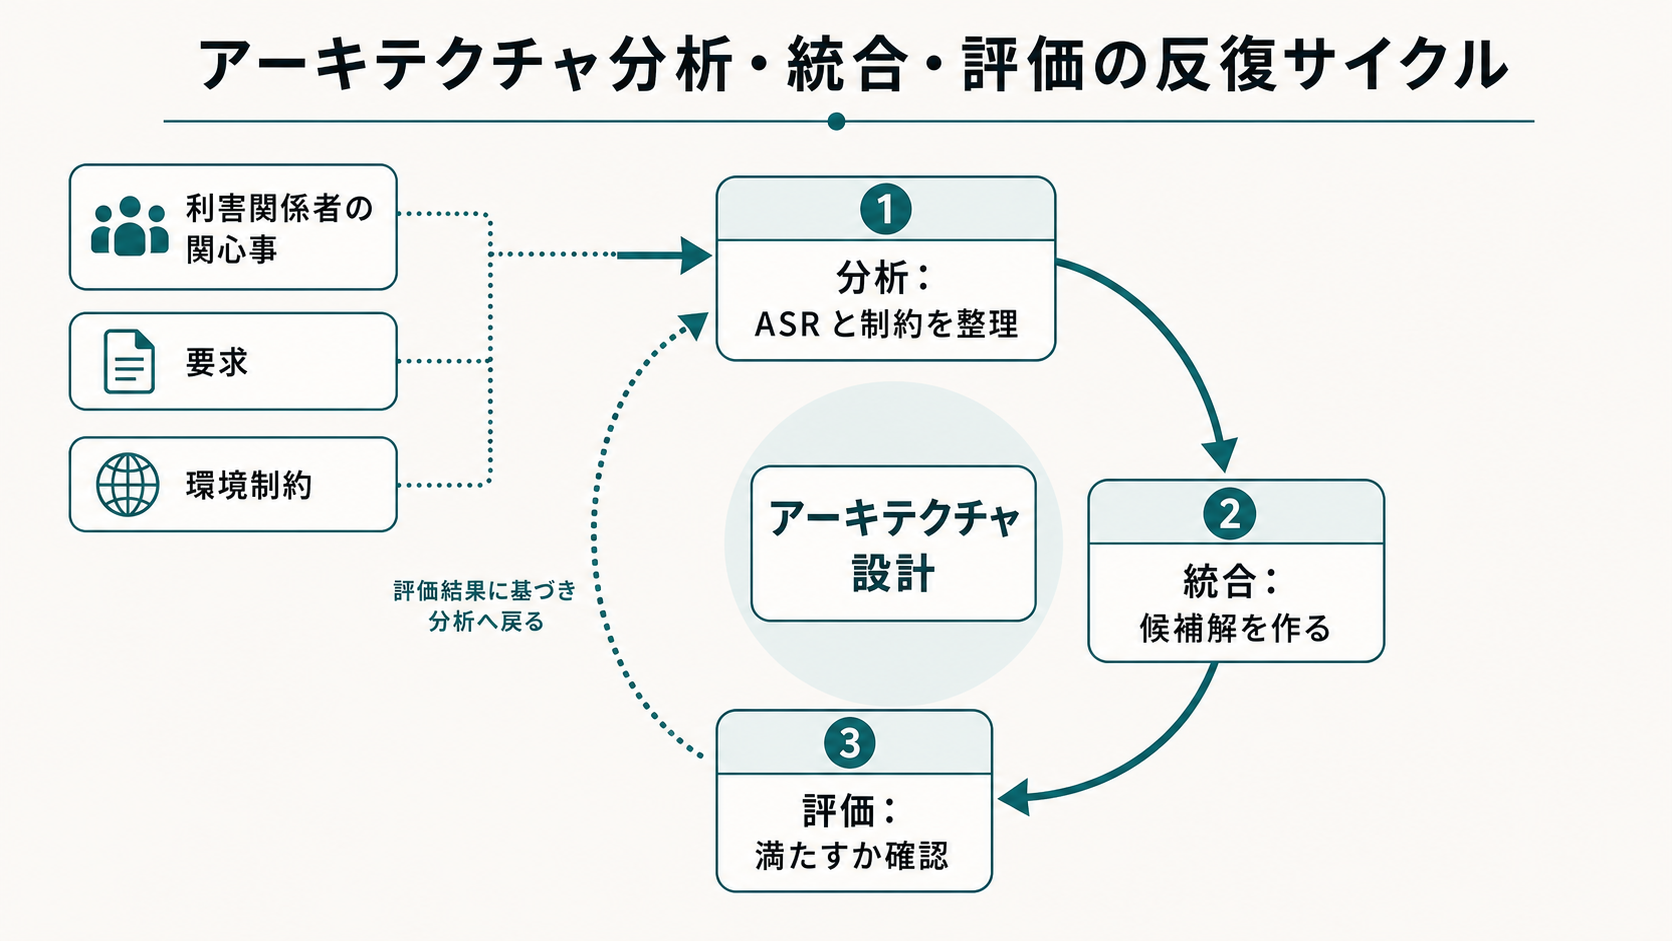
\includegraphics[width=0.96\linewidth]{assets/generated_figures/ch02/fig-ch02-07.png}}{\fbox{\parbox[c][48mm][c]{0.9\linewidth}{\centering 画像生成待ち\\アーキテクチャ分析・統合・評価の反復サイクル}}}
\caption{アーキテクチャ分析・統合・評価の反復サイクル}
\label{fig:ch02-07}
\end{figure}

\subsubsection{アーキテクチャの実践、方法、戦術}
アーキテクチャの実践には、多くの方法がある。方法とは、関心事の発見、要求整理、候補解作成、文書化、レビュー、評価をどの順序で行うかを定める作業手順である。戦術とは、特定の品質特性を満たすための小さな設計上の手段である。

たとえば、可用性を高めるには冗長化、監視、障害切替が使われることがある。性能を高めるにはキャッシュ、非同期処理、並列化が使われることがある。変更容易性を高めるには抽象化、疎結合、情報隠蔽が使われることがある。セキュリティを高めるには認証、認可、入力検証、監査ログが使われることがある。

\begin{statementbox}{注意}
戦術は魔法の解決策ではない。どの戦術にも副作用がある。キャッシュは性能を高めるが、整合性管理を難しくすることがある。冗長化は可用性を高めるが、費用と運用複雑性を増やすことがある。
\end{statementbox}

\subsubsection{大規模なアーキテクチャ活動}
アーキテクチャ設計は、ライフサイクル上の一段階を指すことがある。しかし、広い意味のアーキテクティングは、それだけではない。大規模な組織やシステムでは、個別システムのアーキテクチャが、企業アーキテクチャ、製品系列アーキテクチャ、システム・オブ・システムズのアーキテクチャと関係する。

このような文脈では、次の活動が重要になる。
\begin{itemize}
  \item \keyterm{アーキテクチャ実装管理}：実装がアーキテクチャに従っているかを確認する。
  \item \keyterm{アーキテクチャ保守}：実装後もアーキテクチャを管理し、拡張する。
  \item \keyterm{アーキテクチャ管理}：組織内の複数アーキテクチャの関係を管理する。
  \item \keyterm{アーキテクチャ知識管理}：意思決定、教訓、仕様、文書などを再利用可能な資産として残す。
\end{itemize}

大規模なアーキテクチャ活動では、個別システムの最適化だけでは不十分である。組織全体で一貫性、相互運用性、再利用性、進化可能性を保つ必要がある。

\subsection{ソフトウェアアーキテクチャ評価}

\subsubsection{アーキテクチャにおける「よさ」}
アーキテクチャの「よさ」は、一つの尺度だけでは測れない。ある利害関係者にとってよいアーキテクチャが、別の利害関係者にとっては問題を含むことがある。たとえば、セキュリティを非常に強くした構成は安全に見えるが、費用が高く、検証が難しく、利用者の操作が複雑になることがある。

建築の古典的な考え方では、建物には強さ、用、見た目のよさが必要だとされる。この考え方をソフトウェアに置き換えると、次の問いになる。
\begin{itemize}
  \item 長期運用と進化に耐えられるか。
  \item 意図した用途に合っているか。
  \item このアーキテクチャで、費用対効果よく構築できるか。
  \item 構築、利用、保守を行う人にとって明確で理解しやすいか。
\end{itemize}

\keyterm{アーキテクチャトレードオフ分析法}\en{Architecture Tradeoff Analysis Method, ATAM}は、品質特性に基づいてアーキテクチャを評価する方法である。品質特性を整理し、シナリオを使って評価し、品質要求同士のトレードオフを分析する。ほかにも、ソフトウェアアーキテクチャ分析法\en{SAAM}や品質特性ワークショップ\en{QAW}などの方法がある。

\begin{statementbox}{評価の本質}
評価の目的は、アーキテクチャに点数を付けることだけではない。重大なリスク、隠れた前提、品質特性間の衝突、説明できない判断を早く発見することである。
\end{statementbox}

\subsubsection{アーキテクチャについての推論}
アーキテクチャ評価は、明確なアーキテクチャ記述があるほど効果的である。ビュー、モデル、意思決定記録があれば、それらを調べ、質問し、分析できる。信頼性、安全性、セキュリティのような専門的関心事では、それぞれの分野で使われる専門的な表現が必要になることがある。

しかし、現実にはアーキテクチャ文書が未完成、不完全、古い、存在しない場合も多い。その場合、評価は関係者の知識に依存する。これは危険である。なぜなら、人の記憶は抜け落ちやすく、関係者が退職すると知識も失われるからである。

ユースケースは、アーキテクチャの完全性と整合性を確認する手段として使える。ユースケースの各ステップを見て、そのステップを実現する構成要素がアーキテクチャに存在するか、必要な通信やデータが説明されているかを確認する。

\begin{figure}[htbp]
\centering
\IfFileExists{assets/generated_figures/ch02/fig-ch02-08.png}{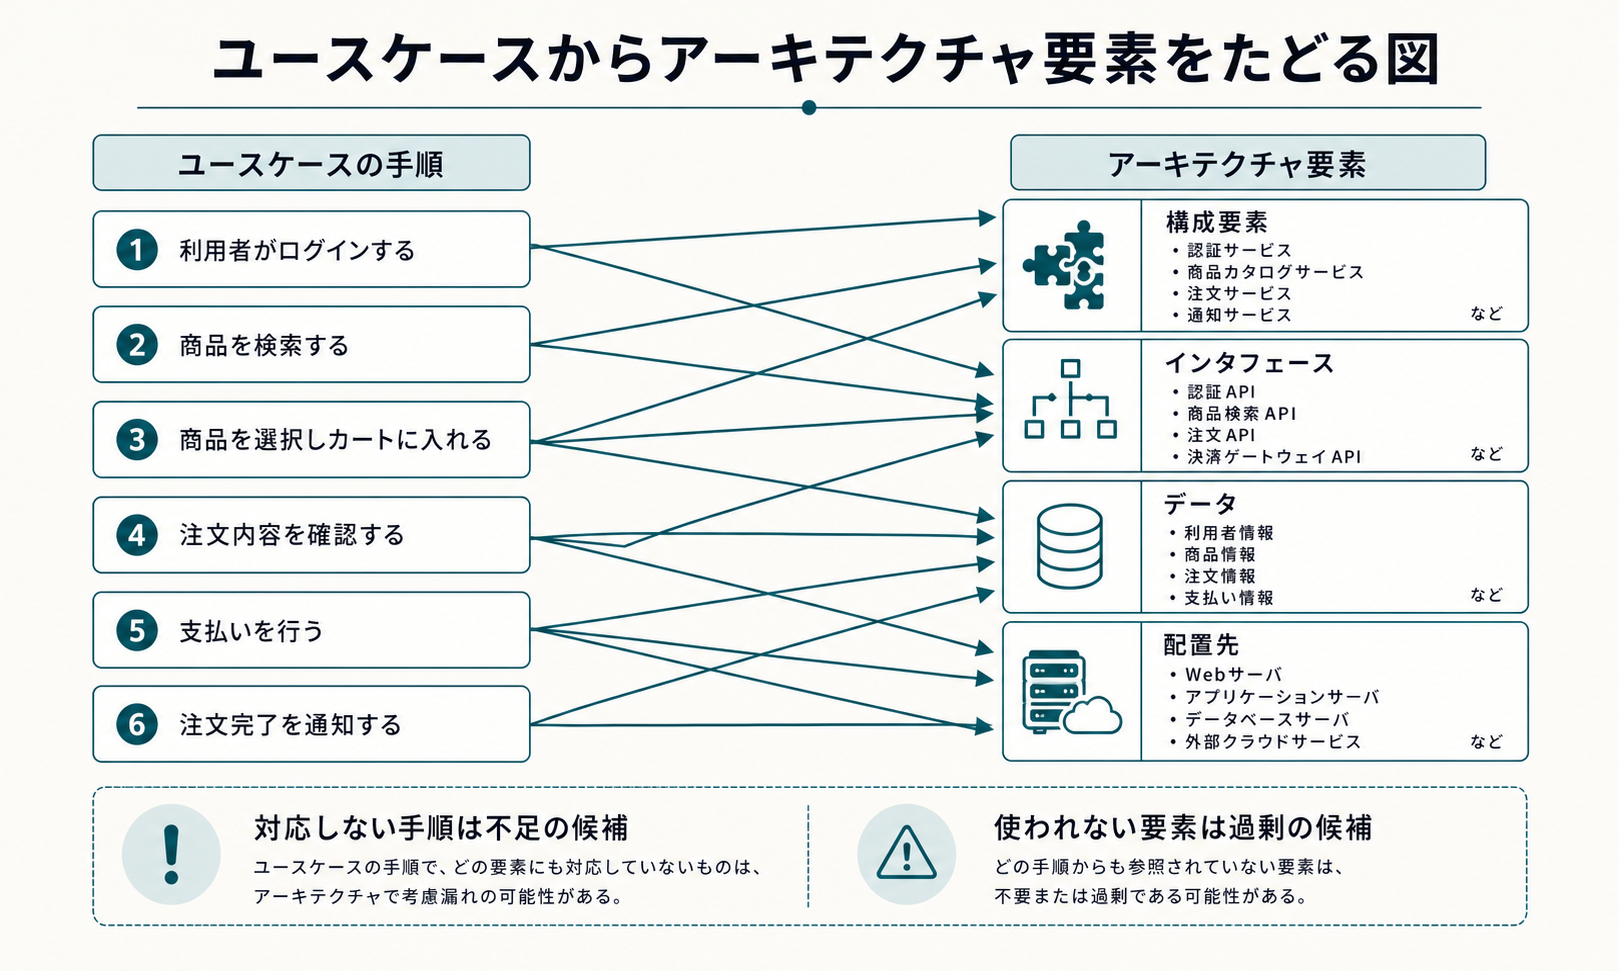
\includegraphics[width=0.96\linewidth]{assets/generated_figures/ch02/fig-ch02-08.png}}{\fbox{\parbox[c][48mm][c]{0.9\linewidth}{\centering 画像生成待ち\\ユースケースからアーキテクチャ要素をたどる図}}}
\caption{ユースケースからアーキテクチャ要素をたどる図}
\label{fig:ch02-08}
\end{figure}

\subsubsection{アーキテクチャレビュー}
アーキテクチャレビューは、アーキテクチャの状態、品質、リスクを確認するための有効な方法である。レビューは、非公式な専門家レビューとして行われることもあれば、チェックリストに基づいて構造化されることもある。

より能動的なレビューでは、単に「この項目を確認したか」と聞くのではなく、レビュアが特定の活動を行って情報を得る。たとえば、「障害が発生したときに、どの構成要素がどの順で影響を受けるかを説明する」「利用者数が 10 倍になったときに、どの構成要素がボトルネックになるかを示す」といった活動である。

\par\smallskip\noindent\refstepcounter{table}\label{tab:ch02-06}\textbf{表 \thetable: 第02章 ソフトウェアアーキテクチャ 表06}\par\smallskip
\begin{longtable}{P{0.25\linewidth}P{0.67\linewidth}}
\toprule
レビュー観点 & 確認すること \\
\midrule
要求対応 & ASR に答える構成や判断があるか。 \\
品質特性 & 性能、可用性、変更容易性、安全性、セキュリティなどが説明されているか。 \\
トレードオフ & ある品質を優先したことで、別の品質にどのような影響があるか。 \\
リスク & 未検証の前提、難しい技術、外部依存、単一障害点があるか。 \\
説明可能性 & 重要な意思決定に根拠が残っているか。 \\
実装適合性 & 実装がアーキテクチャに従っているか、または逸脱が管理されているか。 \\
\bottomrule
\end{longtable}

\subsubsection{アーキテクチャ測度}
\keyterm{アーキテクチャ測度}\en{architecture metrics}とは、アーキテクチャの性質を数量で表すものである。測度は万能ではないが、複雑さ、依存関係、変更リスク、規約適合性を把握する手がかりになる。

代表的な測度には、構成要素間依存、循環依存、循環的複雑度、内部モジュール複雑度、結合度、凝集度、ネストの深さ、パターン・様式・API への準拠などがある。

継続的開発や DevOps の文脈では、アーキテクチャそのものではなく、アーキテクチャの状態を反映する過程測度も使われる。変更リードタイム、配置頻度、サービス復旧平均時間、変更失敗率などである。変更が遅く、復旧が難しく、失敗率が高い場合、アーキテクチャが変更や運用に適していない可能性がある。

\begin{figure}[htbp]
\centering
\IfFileExists{assets/generated_figures/ch02/fig-ch02-09.png}{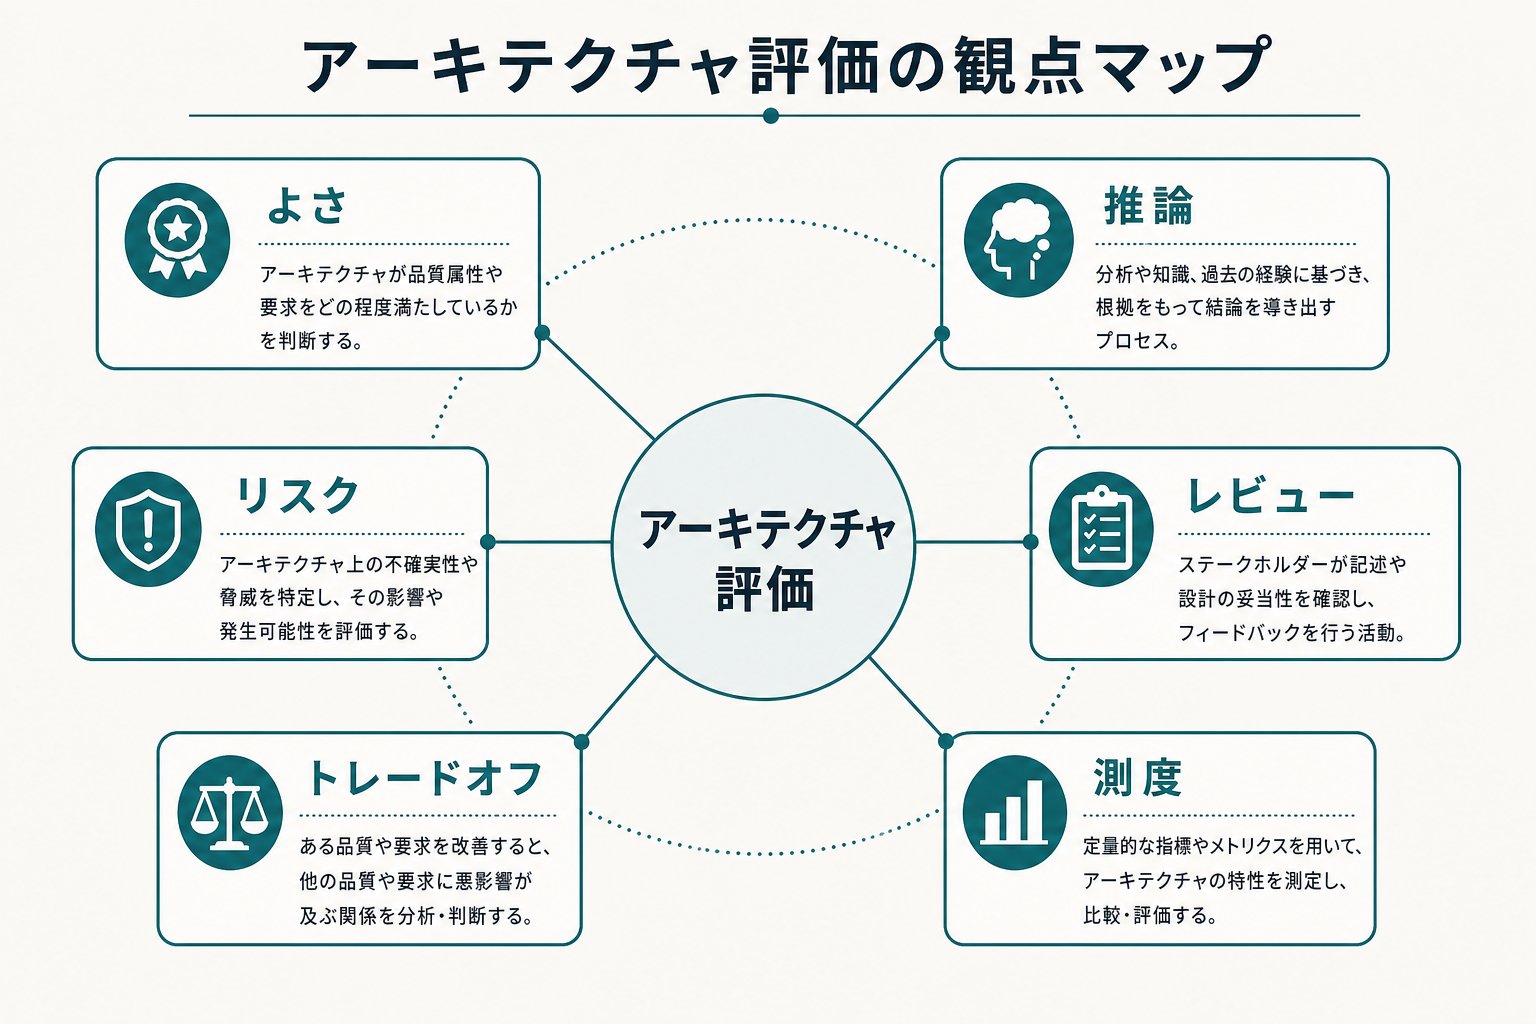
\includegraphics[width=0.96\linewidth]{assets/generated_figures/ch02/fig-ch02-09.png}}{\fbox{\parbox[c][48mm][c]{0.9\linewidth}{\centering 画像生成待ち\\アーキテクチャ評価の観点マップ}}}
\caption{アーキテクチャ評価の観点マップ}
\label{fig:ch02-09}
\end{figure}

\subsection{トピックと参考文献の対応}
この表は、SWEBOK が示す「トピック対参考資料の行列」を、学習用に簡略化したものである。詳しく学ぶときは、各トピックに対応する文献を読む。

\par\smallskip\noindent\refstepcounter{table}\label{tab:ch02-07}\textbf{表 \thetable: 第02章 ソフトウェアアーキテクチャ 表07}\par\smallskip
\begin{longtable}{P{0.42\linewidth}P{0.50\linewidth}}
\toprule
トピック & 主な参考資料 \\
\midrule
1. ソフトウェアアーキテクチャの基礎 & Bass et al.; Maier and Rechtin; Rozanski and Woods; Taylor et al. \\
1.1 「アーキテクチャ」という語の意味 & Bass et al.; Budgen; Maier and Rechtin \\
1.2 利害関係者と関心事 & Bass et al.; Rozanski and Woods; Taylor et al. \\
1.3 アーキテクチャの用途 & Bass et al.; Rozanski and Woods \\
2. アーキテクチャ記述 & Bass et al.; Rozanski and Woods; Sommerville; Taylor et al. \\
2.1 ビューとビューポイント & Budgen; Maier and Rechtin; Rozanski and Woods; Sommerville \\
2.2 パターン、様式、参照アーキテクチャ & Bass et al.; Budgen; Rozanski and Woods; Sommerville; Taylor et al. \\
2.3 アーキテクチャ記述言語と枠組み & Bass et al.; Maier and Rechtin; Rozanski and Woods; Taylor et al. \\
2.4 重要な意思決定としてのアーキテクチャ & Rozanski and Woods; Sommerville \\
3. アーキテクチャ過程 & Maier and Rechtin; Rozanski and Woods; Taylor et al. \\
3.1 文脈の中のアーキテクチャ & Maier and Rechtin; Taylor et al. \\
3.1.1 アーキテクチャと設計の関係 & Sommerville; Taylor et al. \\
3.2 アーキテクチャ設計 & Bass et al. \\
3.2.1 アーキテクチャ分析 & Bass et al.; Taylor et al. \\
3.2.2 アーキテクチャ統合 & Bass et al. \\
3.2.3 アーキテクチャ評価 & Bass et al.; Rozanski and Woods \\
3.3 実践、方法、戦術 & Bass et al.; Maier and Rechtin; Rozanski and Woods \\
3.4 大規模なアーキテクチャ活動 & Maier and Rechtin; Sommerville \\
4. アーキテクチャ評価 & Bass et al.; Rozanski and Woods; Taylor et al. \\
4.1 アーキテクチャの「よさ」 & Bass et al.; Budgen \\
4.2 アーキテクチャについての推論 & Rozanski and Woods \\
4.3 アーキテクチャレビュー & Bass et al. \\
4.4 アーキテクチャ測度 & Bass et al. \\
\bottomrule
\end{longtable}

\subsection{発展的な読み物}
SWEBOK 02 章で紹介される発展的な読み物を、日本語で読む目的に合わせて整理する。

\par\smallskip\noindent\refstepcounter{table}\label{tab:ch02-08}\textbf{表 \thetable: 第02章 ソフトウェアアーキテクチャ 表08}\par\smallskip
\begin{longtable}{P{0.32\linewidth}P{0.60\linewidth}}
\toprule
文献 & 読むと得られること \\
\midrule
Perry and Wolf & ソフトウェアアーキテクチャ研究の基礎的な考え方を学べる。複数ビュー、アーキテクチャ様式、設計との違いなどの出発点を理解できる。 \\
Bass, Clements and Kazman & 品質特性、アーキテクチャ設計、記述、評価、技術的負債を実務的に学べる。 \\
Kruchten & 4+1 ビューモデルを学べる。論理、開発、プロセス、物理の四つのビューを、シナリオで結びつける考え方である。 \\
Rozanski and Woods & 利害関係者、関心事、ビュー、ビューポイントを使ってアーキテクチャを記述する実践的な方法を学べる。 \\
Taylor, Medvidović and Dashofy & アーキテクチャの基礎、理論、実践を包括的に学べる。実装、配置、非機能特性、信頼とセキュリティも扱う。 \\
Clements et al. & ビューとその種類を使って、アーキテクチャをどう文書化するかを学べる。 \\
Brown & 開発者の視点から、アーキテクチャドライバ、品質、制約、リスク管理を学べる。 \\
Fairbanks & リスク駆動で「必要十分な」アーキテクチャを行う考え方を学べる。軽量でアジャイルな文脈にも合う。 \\
Erder, Pureur and Woods & アジャイル、クラウド、DevOps 時代の継続的アーキテクチャを学べる。セキュリティ、回復性、拡張性にも重点がある。 \\
\bottomrule
\end{longtable}

\subsection{参考文献}
{\small\sloppy
\begin{enumerate}[label={[\arabic*]},leftmargin=2.5em]
\item M. Ali Babar and I. Gorton, ``Software Architecture Review: The State of the Practice,'' IEEE Computer, July 2009.
\item L. Bass, P. Clements, and R. Kazman, \textit{Software Architecture in Practice}, 4th edition, 2021.
\item L. Bass, J. Ivers, M. H. Klein, and P. Merson, \textit{Reasoning Frameworks}, CMU/SEI-2005-TR-007, 2005.
\item F. Brooks, \textit{The Design of Design}, Addison-Wesley, 2010.
\item S. Brown, \textit{Software Architecture for Developers}, Leanpub, 2018.
\item D. Budgen, \textit{Software Design: Creating Solutions for Ill-Structured Problems}, 3rd edition, CRC Press, 2021.
\item F. Buschmann, R. Meunier, H. Rohnert, P. Sommerlad, and M. Stal, \textit{Pattern-Oriented Software Architecture}, John Wiley \& Sons, 1996.
\item H. Cervantes and R. Kazman, \textit{Designing Software Architectures: A Practical Approach}, 2nd edition, Addison-Wesley, 2024.
\item P. Clements et al., \textit{Documenting Software Architecture: Views and Beyond}, 2nd edition, Addison-Wesley, 2011.
\item P. Clements, R. Kazman, and M. Klein, \textit{Evaluating Software Architectures}, Addison-Wesley, 2001.
\item M. E. Conway, ``How Do Committees Invent?'' \textit{Datamation}, 14(4), 28--31, 1968.
\item E. W. Dijkstra, ``On the role of scientific thought,'' 1974.
\item T. Erl, \textit{SOA Design Patterns}, Prentice-Hall, 2009.
\item P. Eeles and P. Cripps, \textit{The Process of Software Architecting}, Addison-Wesley, 2010.
\item M. Erder, P. Pureur, and E. Woods, \textit{Continuous Architecture in Practice: Software Architecture in the Age of Agility and DevOps}, Addison-Wesley, 2021.
\item G. Fairbanks, \textit{Just Enough Software Architecture: A Risk-Driven Approach}, Marshall \& Brainerd, 2010.
\item E. Fernandez-Buglioni, \textit{Security Patterns in Practice: Designing Secure Architectures Using Software Patterns}, Wiley, 2013.
\item R. T. Fielding and R. N. Taylor, ``Principled design of the modern web architecture,'' \textit{ACM Transactions on Internet Technology}, 2(2), 115--150, 2002.
\item M. Fowler, D. Rice, M. Foemmel, E. Hieatt, R. Mee, and R. Stafford, \textit{Patterns of Enterprise Application Architecture}, Addison-Wesley, 2003.
\item C. Hofmeister, P. B. Kruchten, R. L. Nord, H. Obbink, A. Ran, and P. America, ``A general model of software architecture design derived from five industrial approaches,'' \textit{The Journal of Systems and Software}, 80, 106--126, 2007.
\item C. Hofmeister, R. L. Nord, and D. Soni, \textit{Applied Software Architecture}, Addison-Wesley, 2000.
\item ISO/IEC/IEEE 24765:2017, \textit{Systems and Software Engineering - Vocabulary}, 2nd edition, 2017.
\item ISO/IEC/IEEE 42010:2011, \textit{Systems and software engineering - Architecture description}, 2011.
\item R. Kazman, S. Haziyev, A. Yakuba, and D. A. Tamburri, ``Managing Energy Consumption as an Architectural Quality Attribute,'' \textit{IEEE Software}, 35(5), 102--107, 2018.
\item P. B. Kruchten, ``The 4+1 View Model of Architecture,'' \textit{IEEE Software}, 12(6), 1995.
\item P. B. Kruchten, R. L. Nord, and I. Ozkaya, \textit{Managing Technical Debt: Reducing Friction in Software Development}, Addison-Wesley, 2019.
\item Z. Li, P. Liang, and P. Avgeriou, ``Architecture viewpoints for documenting architectural technical debt,'' \textit{Software Quality Assurance}, Elsevier, 2016.
\item A. MacCormack, J. Rusnak, and C. Baldwin, ``Exploring the Duality between Product and Organizational Architectures: A Test of the `Mirroring' Hypothesis,'' \textit{Research Policy}, 41, 1309--1324, 2012.
\item M. W. Maier and E. Rechtin, \textit{The Art of Systems Architecting}, 3rd edition, CRC Press, 2021.
\item N. Medvidović, D. S. Rosenblum, D. F. Redmiles, and J. E. Robbins, ``Modeling software architectures in the Unified Modeling Language,'' \textit{ACM Transactions on Software Engineering and Methodology}, 11(1), 2--57, 2002.
\item H. Obbink et al., \textit{Report on Software Architecture Review and Assessment (SARA)}, version 1.0, 2002.
\item D. L. Parnas, ``On the criteria to be used in decomposing systems into modules,'' \textit{Communications of the ACM}, 15(12), 1053--1058, 1972.
\item D. L. Parnas and D. M. Weiss, ``Active Design Reviews: Principles and Practices,'' Proceedings of the 8th International Conference on Software Engineering, 215--222, 1985.
\item D. Perry and A. Wolf, ``Foundations for the study of software architecture,'' \textit{ACM SIGSOFT Software Engineering Notes}, 17(4), 40--52, 1992.
\item E. Poort and H. van Vliet, ``RCDA: Architecting as a Risk- and Cost Management Discipline,'' \textit{Journal of Systems and Software}, 2012.
\item R. Prieto-Diaz and J. M. Neighbors, ``Module Interconnection Languages,'' \textit{Journal of Systems and Software}, 6(4), 307--334, 1986.
\item C. Richardson, \textit{Microservices Patterns}, Manning Publications, 2019.
\item N. Rozanski and E. Woods, \textit{Software Systems Architecture: Working with Stakeholders Using Viewpoints and Perspectives}, 2nd edition, Addison-Wesley, 2011.
\item M. Shaw and D. Garlan, \textit{Software Architecture: Perspectives on an Emerging Discipline}, Prentice Hall, 1996.
\item I. Sommerville, \textit{Software Engineering}, 10th edition, 2016.
\item R. N. Taylor, N. Medvidović, and E. Dashofy, \textit{Software Architecture: Foundations, Theory, and Practice}, Wiley, 2009.
\item R. Weinreich and G. Buchgeher, ``Towards supporting the software architecture life cycle,'' \textit{The Journal of Systems and Software}, 85, 546--561, 2012.
\end{enumerate}
}

\subsection{章末確認問題}
\begin{enumerate}
  \item 「アーキテクチャ」という語の三つの意味を説明せよ。
  \item 利害関係者と関心事の違いを、自分の言葉で説明せよ。
  \item なぜアーキテクチャ記述では複数のビューを使うのか。
  \item ビューとビューポイントの違いを説明せよ。
  \item アーキテクチャ様式、アーキテクチャパターン、参照アーキテクチャを区別せよ。
  \item アーキテクチャ上重要な要求 ASR の例を三つ挙げよ。
  \item アーキテクチャ根拠を記録する理由を説明せよ。
  \item アーキテクチャ評価で、トレードオフを確認することが重要な理由を説明せよ。
  \item アーキテクチャ測度の例を三つ挙げ、それぞれ何を知るためのものか説明せよ。
\end{enumerate}

\begin{statementbox}{解答の方向性}
1 は三義、2 は主体と論点、3 と 4 は関心事別の表現、5 は型・解決法・領域基準の違いで説明する。6 以降は、性能、可用性、セキュリティ、変更容易性、法規制、外部連携を例にできる。
\end{statementbox}

\section{第03章 ソフトウェア設計}
\begin{pointbox}{この資料の主張}
  ソフトウェア設計は、要求を単に「コードにする前の図」に変換する作業ではない。設計は、要求・制約・利害関係者の関心を、実装でき、評価でき、保守できる解決策へ変換する活動である。設計では、抽象化、関心事の分離、モジュール化、カプセル化、結合度、凝集度などの原則を使って複雑さを扱う。また、設計判断には根拠があり、その根拠を記録することで、後の変更や保守で同じ議論を繰り返さずに済む。
  \end{pointbox}

\begin{pointbox}{この資料の読み方}
  専門用語は原則として日本語で示し、必要に応じて英語を括弧内に併記する。英語名は、元資料やツール上の名称を確認したいときの手がかりとして残す。初学者が前提知識なしに読めるように、各節では「何のための概念か」「設計時に何を決めるのか」「実務では何を確認するのか」を重視する。文体は、だである調で統一する。
  \end{pointbox}





\subsection*{全体概要：この章で学ぶこと}
\addcontentsline{toc}{subsection}{全体概要：この章で学ぶこと}

この章は、ソフトウェア開発における「設計」を扱う。設計は、要求を実装へ橋渡しする中心的な活動である。要求が「何を満たすべきか」を示すなら、設計は「どのような構造と振る舞いで満たすか」を示す。設計は、プログラムを書く前の一時的な準備だけではなく、保守、変更、品質評価、テスト、認証にも影響する長期的な知識資産である。

\textbf{到達目標} この章を読み終えると、次のことができるようになる。
\begin{itemize}
  \item ソフトウェア設計の意味を、設計という分野、設計活動、設計結果、ライフサイクル上の段階として説明できる。
  \item 設計思考、設計文脈、主要論点、設計原則の役割を説明できる。
  \item 高水準設計と詳細設計の違いを説明できる。
  \item 並行性、イベント処理、データ永続化、分散、例外処理、統合、安全性、変動性など、設計品質の観点を説明できる。
  \item 構造設計記述と振る舞い設計記述の代表的な記法を見分けられる。
  \item 設計パターン、領域固有言語、設計根拠、設計レビュー、設計メトリクスの意味を説明できる。
\end{itemize}

\textbf{学習順序} 初学者は、まず「設計は何を変換する活動か」を押さえる。その後、「よい設計の原則」「設計の段階」「設計で扱う品質」「設計をどう記録するか」「設計方法の違い」「設計をどう評価するか」の順に読むとよい。

\begin{figure}[htbp]
\centering
\IfFileExists{assets/generated_figures/ch03/fig-ch03-01.png}{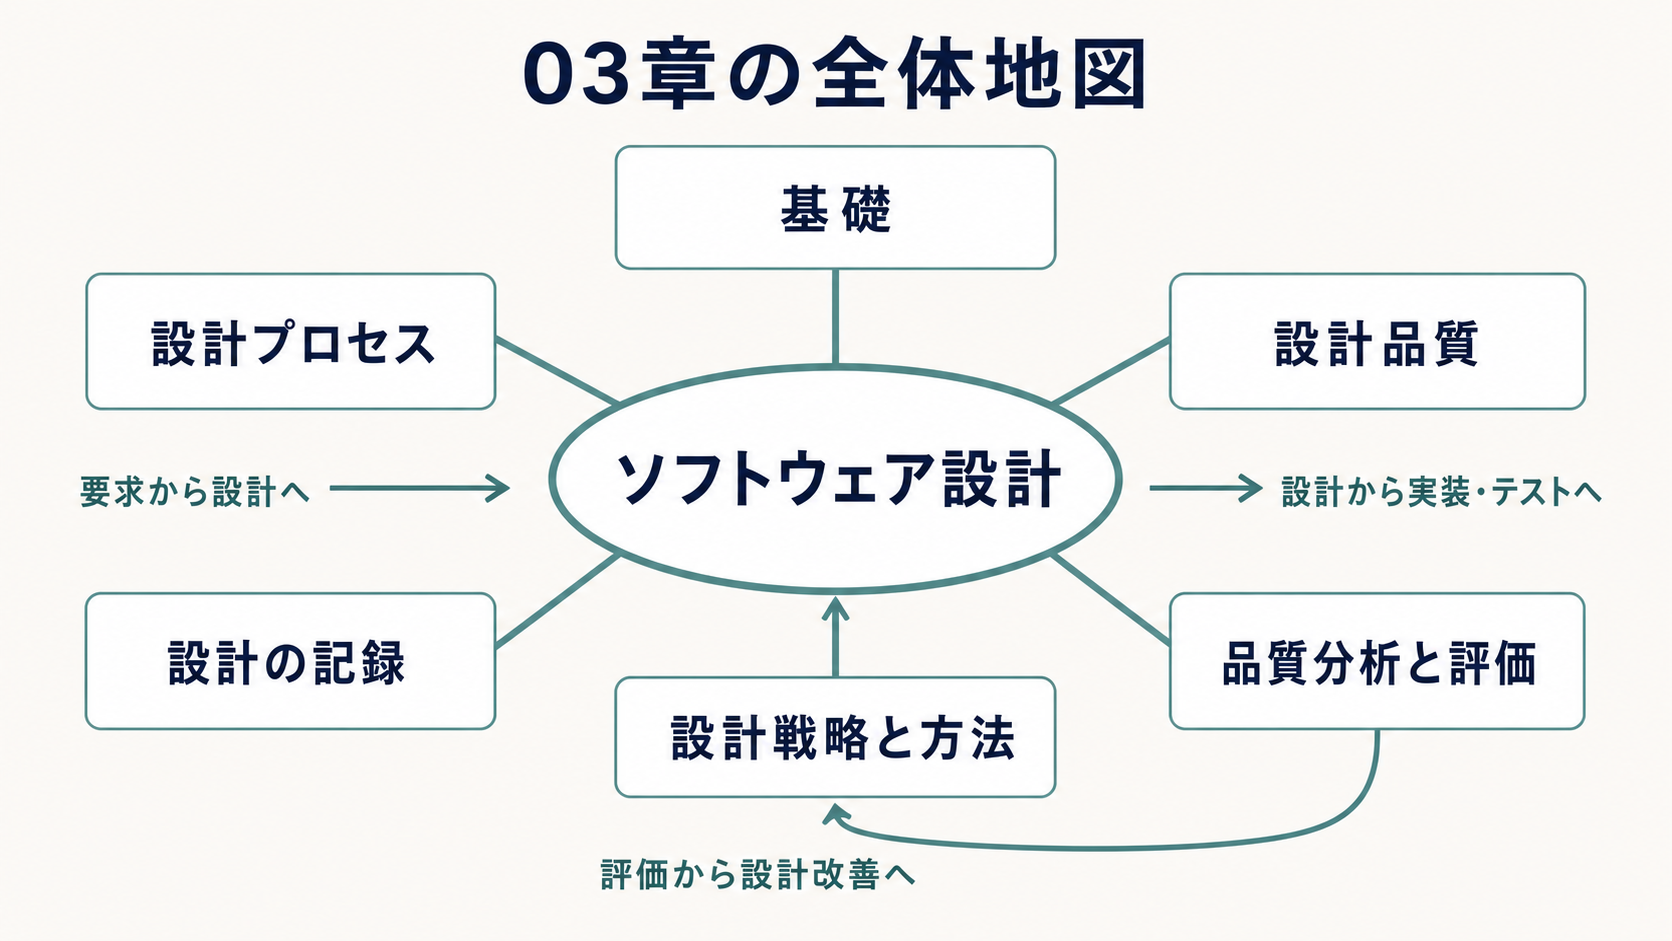
\includegraphics[width=0.96\linewidth]{assets/generated_figures/ch03/fig-ch03-01.png}}{\fbox{\parbox[c][48mm][c]{0.9\linewidth}{\centering 画像生成待ち\\03章の全体地図}}}
\caption{03章の全体地図}
\label{fig:ch03-01}
\end{figure}

\subsection*{最初に必要な用語}
\addcontentsline{toc}{subsection}{最初に必要な用語}

\par\smallskip\noindent\refstepcounter{table}\label{tab:ch03-01}\textbf{表 \thetable: 第03章 ソフトウェア設計 表01}\par\smallskip
\begin{tabularx}{\linewidth}{L{34mm}Y}
\toprule
\textbf{用語} & \textbf{初学者向けの説明} \\
\midrule
ソフトウェア設計 & 要求、制約、品質目標を、実装できる構造・振る舞い・インタフェースへ変換する活動である。 \\
設計記述 & 設計結果を記録した文書、モデル、図、表、プロトタイプなどである。英語では Software Design Description、略して SDD と呼ぶ。 \\
構成要素 & システムを構成する部品である。部品は、モジュール、クラス、サービス、コンポーネントなどの形を取る。 \\
インタフェース & ある構成要素が外部とやり取りする接点である。入力、出力、呼び出し方、データ形式、例外条件などを含む。 \\
抽象化 & 注目したい情報だけを取り出し、不要な詳細を隠す考え方である。複雑さを下げるために使う。 \\
モジュール化 & 大きなソフトウェアを、名前を持つ小さな部品に分けることである。理解、分担、保守を容易にする。 \\
カプセル化 & 部品の内部詳細を隠し、外部からは必要な操作だけを見せることである。情報隠蔽とも呼ぶ。 \\
品質属性 & 性能、信頼性、保守容易性、セキュリティ、使いやすさなど、ソフトウェアの性質である。 \\
トレードオフ & ある性質を高めると、別の性質や費用に悪影響が出る関係である。設計では避けられない。 \\
設計根拠 & なぜその設計判断をしたかという理由である。代替案、前提、制約、採用理由、却下理由を含む。 \\
\bottomrule
\end{tabularx}

\subsubsection*{略語}
\addcontentsline{toc}{subsubsection}{略語}

\par\smallskip\noindent\refstepcounter{table}\label{tab:ch03-02}\textbf{表 \thetable: 第03章 ソフトウェア設計 表02}\par\smallskip
\begin{tabularx}{\linewidth}{L{18mm}L{43mm}Y}
\toprule
\textbf{略語} & \textbf{日本語} & \textbf{説明} \\
\midrule
API & アプリケーションプログラミングインタフェース & ソフトウェア部品やサービスを外部から利用するための呼び出し規約である。 \\
AOD & アスペクト指向設計 & 横断的関心事をアスペクトとして扱う設計方法である。 \\
CBD & 構成要素ベース設計 & 独立した構成要素を組み合わせてシステムを作る方法である。 \\
CRC & クラス・責務・協調カード & クラス名、責務、協調相手をカード形式で整理する方法である。 \\
DFD & データフロー図 & データの流れと処理を表す図である。 \\
DSL & 領域固有言語 & 特定領域の概念を直接表すための専用言語である。 \\
ERD & 実体関連図 & データの実体と関係を表す図である。 \\
FOSS & 自由・オープンソースソフトウェア & ソースコード利用、変更、再配布が許されるソフトウェアである。 \\
IDL & インタフェース記述言語 & 構成要素のインタフェースを記述する言語である。 \\
MBD & モデルに基づく設計 & モデルを設計記録の中心に置く方法である。 \\
MDD & モデル駆動開発 & モデルを主要成果物とし、実装やテストへつなげる開発方法である。 \\
OO & オブジェクト指向 & データと操作を持つオブジェクトを中心に考える方法である。 \\
PDL & プログラム設計言語 & プログラムに近い擬似言語で処理を表す記法である。 \\
SDD & ソフトウェア設計記述 & 設計情報を伝達・分析・実装に使うための記録である。 \\
SoC & 関心事の分離 & 複数の観点を分けて考え、複雑さを下げる原則である。 \\
UML & 統一モデリング言語 & 構造や振る舞いを表すための代表的なモデリング記法群である。 \\
\bottomrule
\end{tabularx}

\subsection*{導入：設計とは何か}
\addcontentsline{toc}{subsection}{導入：設計とは何か}

ソフトウェア設計という語は、近いが異なる意味で使われる。第一に、設計は分野である。これは、科学的原理、技術情報、想像力を使って、目的を満たすソフトウェアを経済的かつ効率的に定義する分野である。第二に、設計はその分野の中で行われるプロセスである。第三に、設計はプロセスの結果、つまり設計記述やモデルである。第四に、設計はライフサイクル上の段階でもある。

\term{ソフトウェア設計記述}{Software Design Description, SDD} は、設計情報を伝えるための成果物である。これは、実装、計画、分析、意思決定を助ける「青写真」に相当する。設計記述には、ソフトウェアを構成要素へ分けること、構成要素をどのように配置するか、構成要素同士と外部世界とのインタフェースをどのように定義するかが含まれる。

ソフトウェア設計は、要求を分析し、外部から見える性質と内部構造を定める活動である。設計は、一般に三段階で考えると理解しやすい。第一はアーキテクチャ設計であり、システム全体の根本的な構造と原則を扱う。第二は高水準設計であり、システムと主要構成要素が外部とどう関わるかを扱う。第三は詳細設計であり、各構成要素の内部を実装できる水準まで具体化する。

\begin{pointbox}{重要}
設計は「実装前にきれいな図を描くこと」ではない。設計は、要求、制約、品質目標、技術選択、保守の見通しを踏まえ、作れる解決策を定義する活動である。
\end{pointbox}

\subsection{ソフトウェア設計の基礎}

ソフトウェア設計の基礎は、設計を理解するための概念、用語、判断基準である。初学者にとって重要なのは、設計を「コードを書く前の一工程」と狭く見るのではなく、「問題を解決可能な形へ変換する思考」として見ることである。

\subsubsection{設計思考}

\term{設計思考}{Design Thinking} は、必要や問題を理解し、それに対する解決策を考える思考である。設計対象はソフトウェアに限らない。建築、工業製品、組織、業務手順など、人が目的を持って作るものには設計が関わる。

ソフトウェア設計で重要なのは、問題と解決策を表す語彙を作ることである。ソフトウェアは、物理的な材料を削って作るものではなく、概念、名前、規則、手続き、データ、インタフェースを組み合わせて作る。したがって、設計は言語的な活動でもある。

設計思考は、次の五段階として理解できる。
\begin{enumerate}
  \item 目的や目標を明確にする。
  \item その目的を達成する概念的な構造を考える。
  \item 概念構造を実現する仕組みを考える。
  \item その仕組みを表し、利用するための記法や語彙を作る。
  \item 具体的な問題文脈で記法を使い、目的を達成する。
\end{enumerate}

\begin{definitionbox}
設計思考とは、問題を理解し、制約の中で複数の解決策を考え、根拠を持って選び、表現可能な形へまとめる思考である。
\end{definitionbox}

\begin{figure}[htbp]
\centering
\IfFileExists{assets/generated_figures/ch03/fig-ch03-02.png}{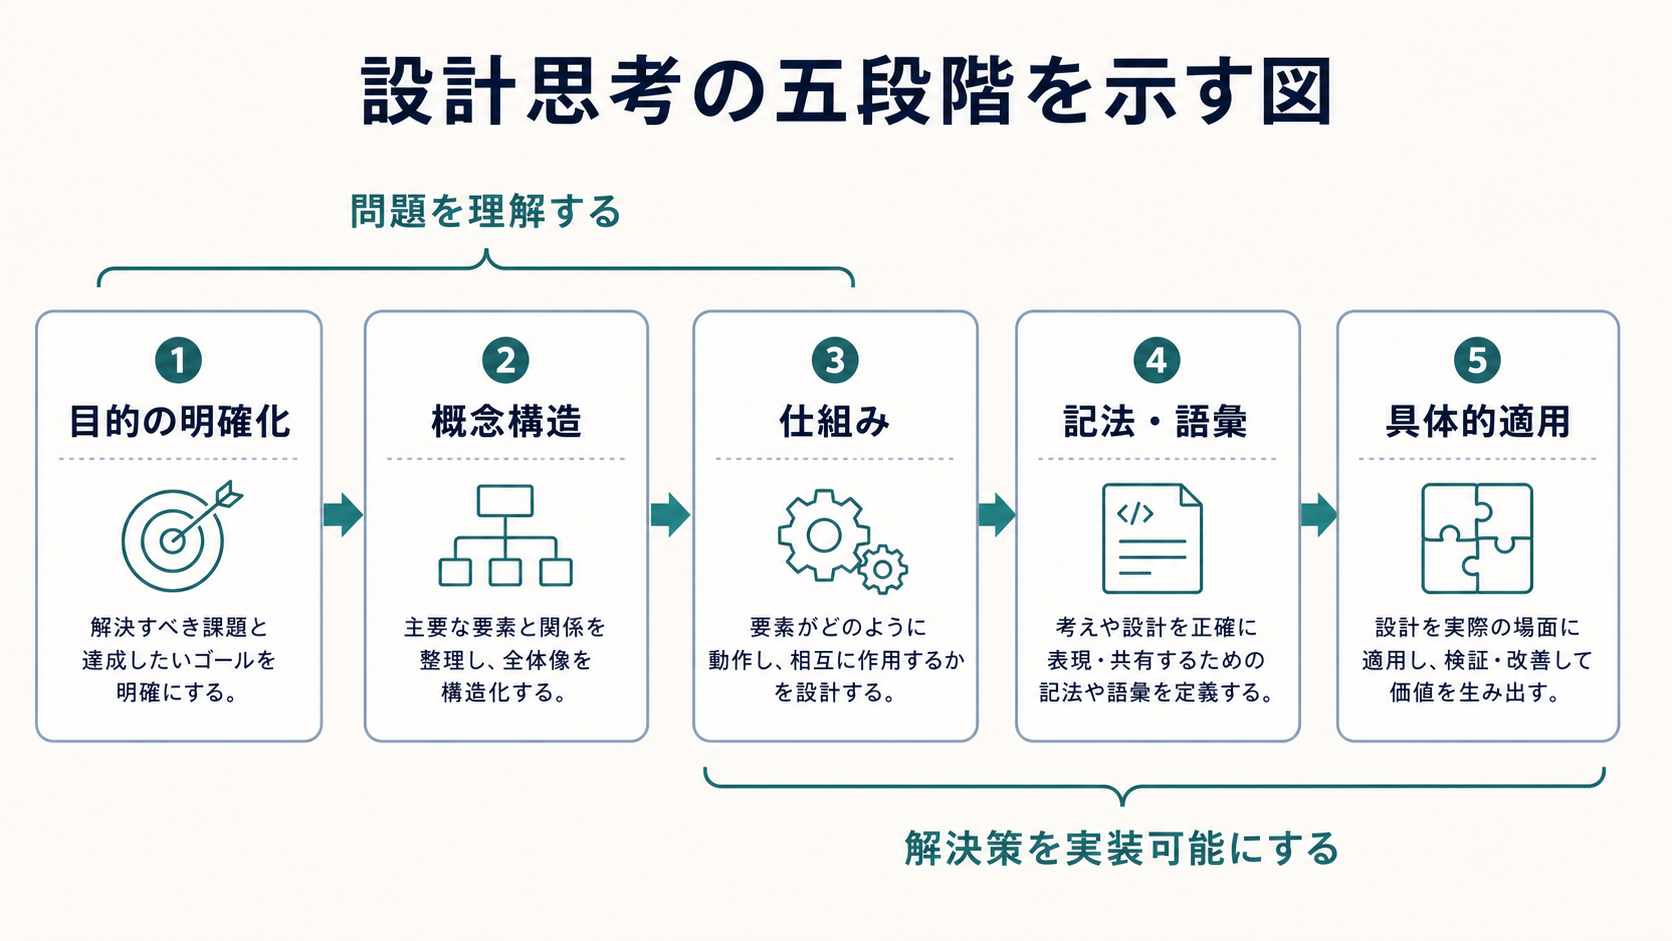
\includegraphics[width=0.96\linewidth]{assets/generated_figures/ch03/fig-ch03-02.png}}{\fbox{\parbox[c][48mm][c]{0.9\linewidth}{\centering 画像生成待ち\\設計思考の五段階を示す図}}}
\caption{設計思考の五段階を示す図}
\label{fig:ch03-02}
\end{figure}

\subsubsection{ソフトウェア設計の文脈}

ソフトウェア設計は、開発ライフサイクルの中で孤立して存在しない。要求、アーキテクチャ、実装、テスト、保守と強くつながっている。

\begin{itemize}
  \item \textbf{要求との関係}：要求は、設計が解くべき問題を示す。設計は、要求を実装可能な構造と振る舞いへ変換する。
  \item \textbf{アーキテクチャとの関係}：アーキテクチャが定められている場合、それは設計の制約となる。主要構成要素、接続、API、採用すべきスタイルやパターン、設計原則などを制約する。
  \item \textbf{実装との関係}：設計は、実装者が何を作るべきかを示す案内である。実装者がコードを読む前に、部品の責務やインタフェースを理解できることが望ましい。
  \item \textbf{テストとの関係}：設計は、テスト戦略とテストケースの土台になる。設計要素が要求をどう満たすかが明らかであれば、テストの観点も作りやすい。
\end{itemize}

設計の形式性は、プロジェクトによって異なる。安全性が重要なシステムでは、設計記述を厳密に残す必要がある。一方、小規模な探索的開発では、簡潔なモデルやコードそのものが設計記録の中心になる場合もある。ただし、どの場合でも、関係者が設計判断を理解できることが重要である。

\begin{figure}[htbp]
\centering
\IfFileExists{assets/generated_figures/ch03/fig-ch03-03.png}{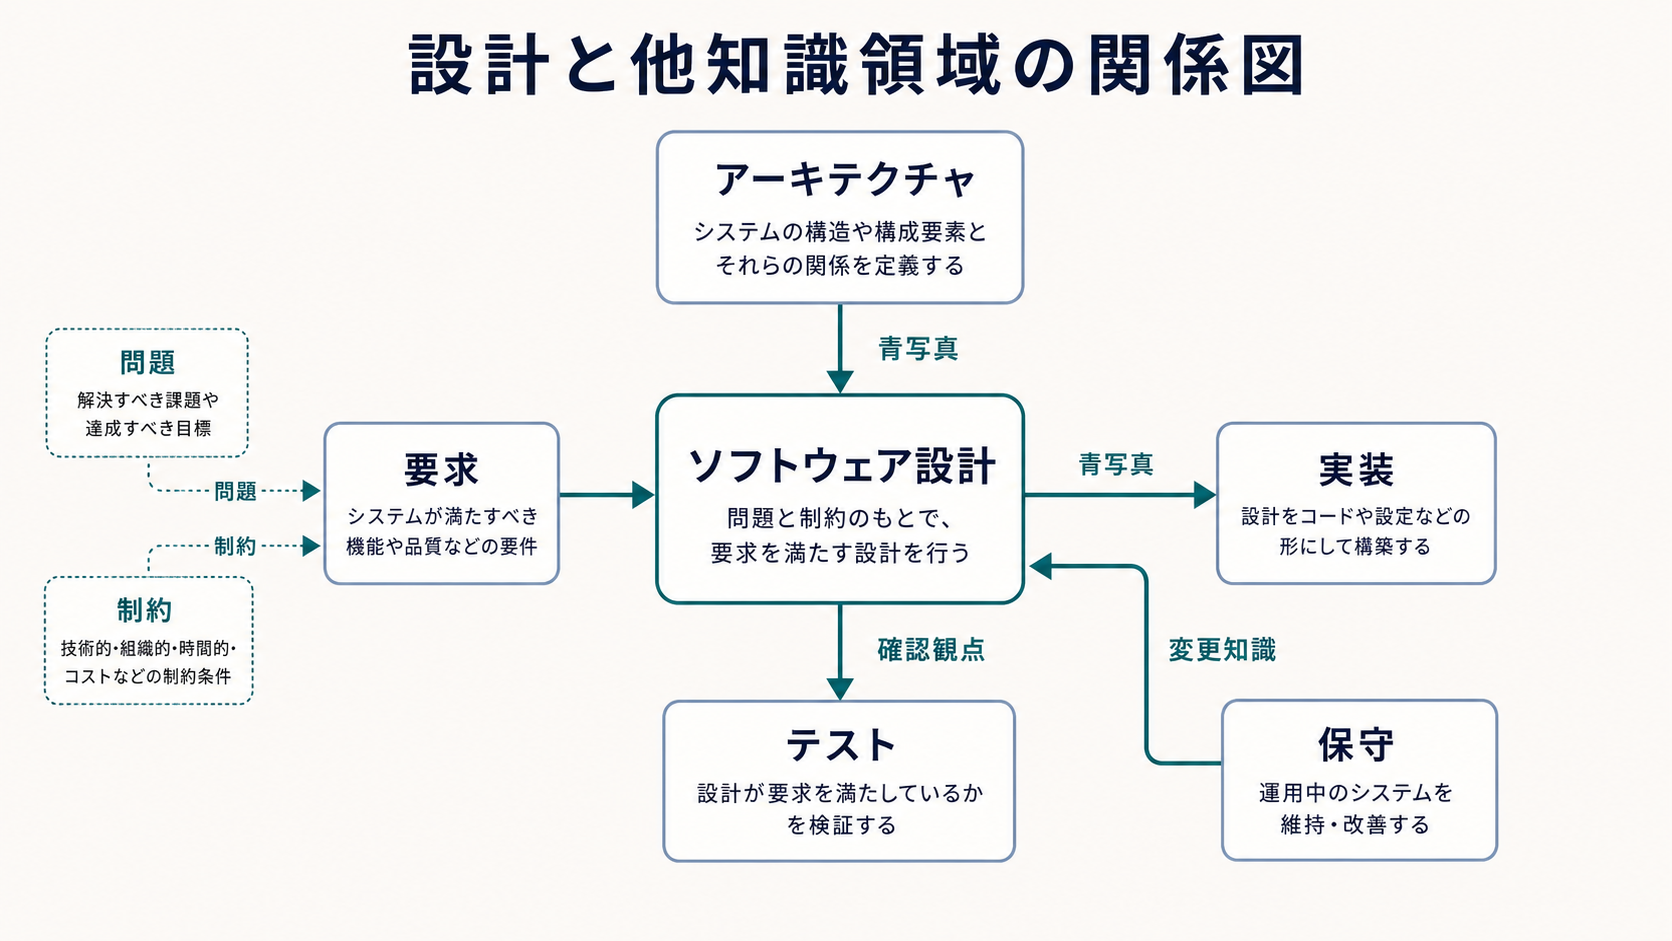
\includegraphics[width=0.96\linewidth]{assets/generated_figures/ch03/fig-ch03-03.png}}{\fbox{\parbox[c][48mm][c]{0.9\linewidth}{\centering 画像生成待ち\\設計と他知識領域の関係図}}}
\caption{設計と他知識領域の関係図}
\label{fig:ch03-03}
\end{figure}

\subsubsection{ソフトウェア設計の主要論点}

設計では、多くの論点を同時に扱う必要がある。代表的な論点は、性能、セキュリティ、信頼性、使いやすさ、保守容易性などの品質である。また、ソフトウェアをどのような構成要素へ分けるか、それらをどう接続するか、どの単位で責務を持たせるかも重要である。

設計論点には、機能そのものではないが、システム全体に影響するものもある。たとえば、ログ、認証、監査、例外処理、キャッシュ、トランザクション、セキュリティ確認などは、多くの機能に横断的に関わる。こうした論点は\term{横断的関心事}{crosscutting concern} と呼ばれる。

\begin{pointbox}{注意}
横断的関心事を場当たり的に実装すると、同じ処理が各所に重複し、変更時に漏れが起きやすくなる。設計段階で共通方針を決めることが重要である。
\end{pointbox}

\subsubsection{ソフトウェア設計原則}

設計原則は、設計中の判断に方向を与える基本的な考え方である。原則は、特定のプログラミング言語や開発手法だけに依存しない。むしろ、複雑な問題を扱うための共通の知恵である。

\par\smallskip\noindent\refstepcounter{table}\label{tab:ch03-03}\textbf{表 \thetable: 第03章 ソフトウェア設計 表03}\par\smallskip
\begin{longtable}{L{34mm}L{55mm}L{76mm}}
\toprule
\textbf{原則} & \textbf{意味} & \textbf{実務で見ること} \\
\midrule
\endhead
抽象化 & 目的に関係する情報だけを示し、不要な詳細を隠す。 & 利用者、設計者、実装者が必要な詳細水準だけを見られるか。 \\
関心事の分離 & 異なる関心を分けて扱う。 & 業務処理、認証、ログ、表示、保存などが混ざりすぎていないか。 \\
モジュール化 & 大きなソフトウェアを小さな部品へ分ける。 & 各部品の責務が明確で、独立して理解・変更できるか。 \\
カプセル化・情報隠蔽 & 内部詳細を隠し、必要なインタフェースだけを見せる。 & 外部が内部データ構造や実装順序に依存していないか。 \\
インタフェースと実装の分離 & 外部に見せる契約と内部実装を分ける。 & 実装を変えても、利用側の変更が少なく済むか。 \\
結合度 & 部品同士の依存の強さである。 & ひとつの部品変更が多数の部品変更を引き起こさないか。 \\
凝集度 & ひとつの部品内の要素がどれだけ関連しているかである。 & ひとつの部品が複数の無関係な責務を抱えていないか。 \\
一貫性 & 名前、記法、順序、インタフェースなどをそろえる。 & 似た問題に似た解決策を使っているか。 \\
完全性 & 重要な特徴や要求を漏らさない。 & 通常時、例外時、境界条件、状態、モードが考慮されているか。 \\
検証可能性 & 要求や制約を満たすか確認できる。 & 設計からテスト、レビュー、分析が可能か。 \\
倫理的配慮 & 人権、福祉、透明性、説明責任、悪用可能性などを考慮する。 & AI、自律システム、社会的影響があるシステムで設計上の配慮があるか。 \\
\bottomrule
\end{longtable}

特に、結合度と凝集度は初学者が最初に押さえるべき設計観点である。一般に、よい設計は、部品間の結合度を低くし、部品内の凝集度を高くする。結合度が高いと変更の影響が広がる。凝集度が低いと、部品が何を担当しているのか理解しにくくなる。

\begin{pointbox}{重要}
設計原則は、単独で使うものではない。抽象化、関心事の分離、モジュール化、カプセル化、低結合、高凝集は互いに支え合う。
\end{pointbox}

\begin{figure}[htbp]
\centering
\IfFileExists{assets/generated_figures/ch03/fig-ch03-04.png}{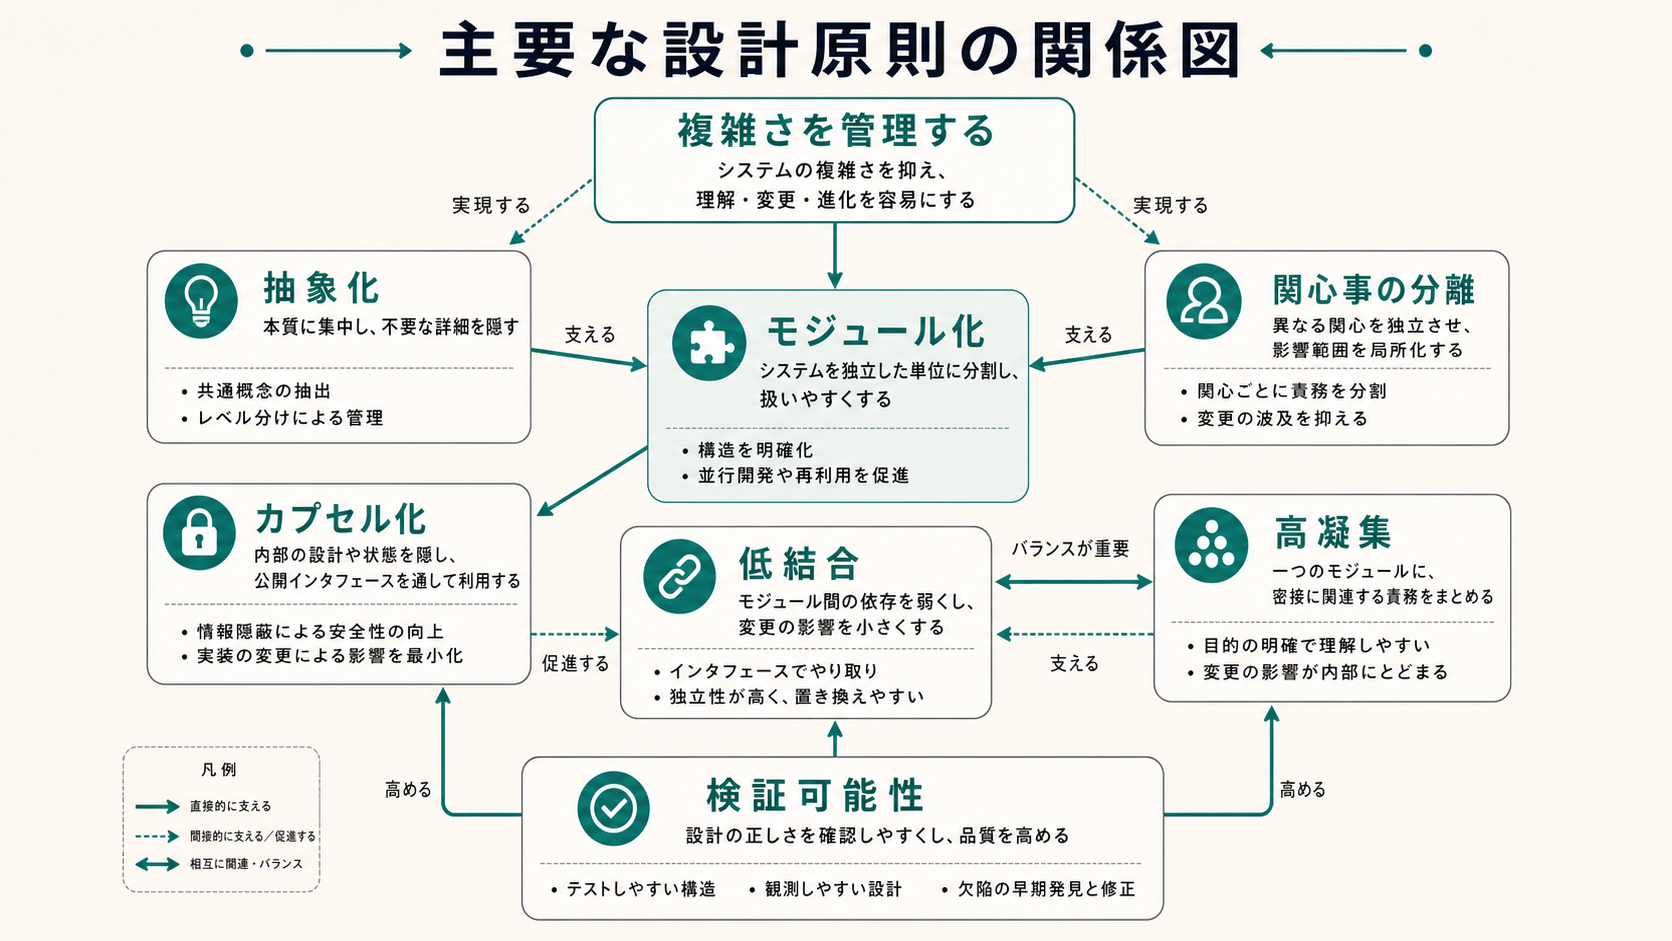
\includegraphics[width=0.96\linewidth]{assets/generated_figures/ch03/fig-ch03-04.png}}{\fbox{\parbox[c][48mm][c]{0.9\linewidth}{\centering 画像生成待ち\\主要な設計原則の関係図}}}
\caption{主要な設計原則の関係図}
\label{fig:ch03-04}
\end{figure}

\subsection{ソフトウェア設計プロセス}

ソフトウェア設計は、一般に多段階の活動として考えられる。段階は、常に厳密に分かれるわけではないが、何を決める段階かを理解すると、設計成果物を作りやすくなる。

設計は、三つの段階に分けられる。
\begin{itemize}
  \item \textbf{アーキテクチャ設計}：システム全体の根本的な構造、主要構成要素、接続方式、支配的な品質方針を決める。
  \item \textbf{高水準設計}：外部に向いた設計であり、主要構成要素と外部環境のやり取り、構成要素間のやり取りを決める。
  \item \textbf{詳細設計}：内部に向いた設計であり、構成要素の内部構造、データ構造、アルゴリズム、内部モジュールを決める。
\end{itemize}

段階の境界は、プロジェクトやシステムの性質で変わる。たとえば、通常ならプログラマが選ぶソートアルゴリズムでも、極端な性能要求があるシステムでは、初期の設計段階で決める必要がある。このように、何をいつ決めるかは、その判断が要求達成にどれほど重要かで決まる。

\begin{figure}[htbp]
\centering
\IfFileExists{assets/generated_figures/ch03/fig-ch03-05.png}{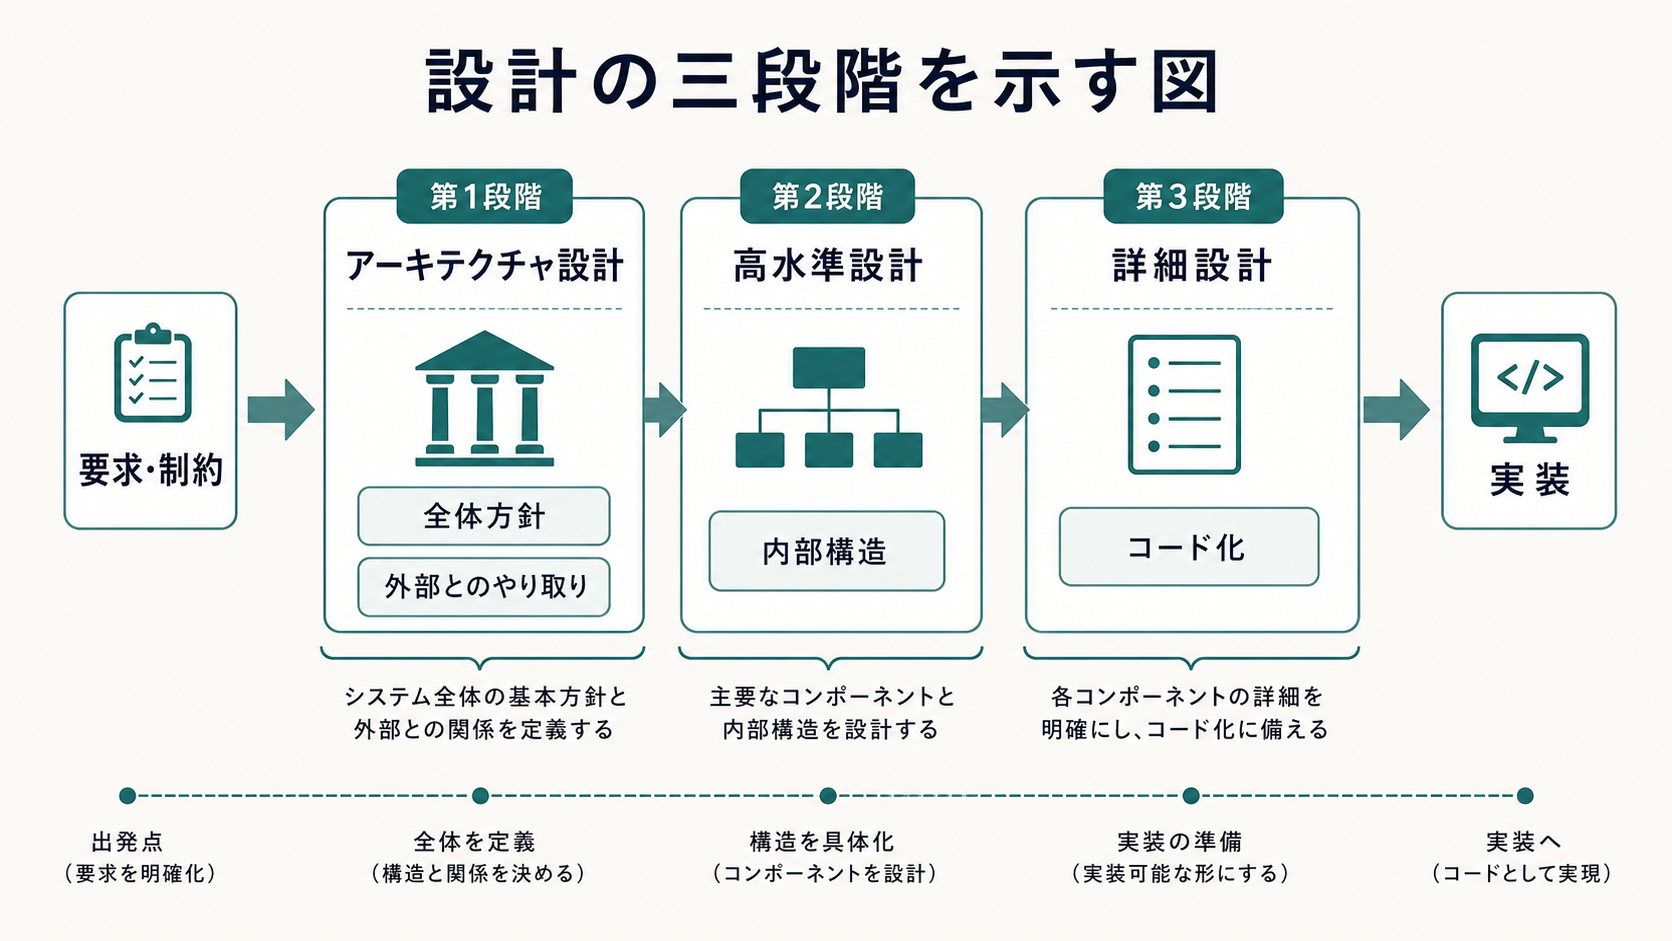
\includegraphics[width=0.96\linewidth]{assets/generated_figures/ch03/fig-ch03-05.png}}{\fbox{\parbox[c][48mm][c]{0.9\linewidth}{\centering 画像生成待ち\\設計の三段階を示す図}}}
\caption{設計の三段階を示す図}
\label{fig:ch03-05}
\end{figure}

\subsubsection{高水準設計}

\term{高水準設計}{High-Level Design} は、システムの主要構成要素が互いにどう関わり、外部環境とどうやり取りするかを決める設計である。外部環境には、利用者、外部システム、デバイス、ネットワーク、データベース、運用環境などが含まれる。

高水準設計では、主に次を扱う。
\begin{itemize}
  \item システムが反応すべき外部イベントやメッセージ。
  \item システムが生成すべきイベントやメッセージ。
  \item イベントやメッセージのデータ形式とプロトコル。
  \item 入力と出力の順序、タイミング、依存関係。
  \item 端から端までの取引やイベント列の流れ。
  \item データをどのように保存し、管理するか。
\end{itemize}

高水準設計は、アーキテクチャがある場合、その枠内で行われる。たとえば、アーキテクチャが「非同期メッセージでやり取りする」と決めていれば、高水準設計ではその方針に従って、具体的なメッセージ種類、順序、例外時の扱いを決める。

\subsubsection{詳細設計}

\term{詳細設計}{Detailed Design} は、主要構成要素の内部を実装できる水準まで具体化する設計である。これは、プログラマがコードを書くための直接的な手がかりになる。

詳細設計では、主に次を扱う。
\begin{itemize}
  \item 主要構成要素を内部モジュールやプログラム単位へ分ける。
  \item 各モジュールの責務を割り当てる。
  \item モジュール間のやり取りを決める。
  \item 名前の有効範囲、可視性、公開・非公開の境界を決める。
  \item 状態、モード、状態遷移を定義する。
  \item データと制御の依存関係を明らかにする。
  \item データ構造、アルゴリズム、ユーザインタフェースの詳細を決める。
\end{itemize}

詳細設計は、実装と完全に分離して行われるとは限らない。特に反復型やアジャイル型の開発では、設計と実装が近い間隔で進む。しかし、その場合でも、設計判断が存在しなくなるわけではない。設計判断がコードの中だけに閉じ込められるのか、明示的に記録されるのかが変わるだけである。

\subsection{ソフトウェア設計品質}

設計品質とは、設計がどのような性質を持つか、またその設計によって作られるソフトウェアがどのような品質を達成しやすいかに関する観点である。ここで扱う品質は、単に「よく動く」ことではなく、並行処理、イベント処理、永続化、分散、例外処理、統合、安全性、変動性など、多面的である。

\subsubsection{並行性}

\term{並行性}{Concurrency} は、複数の処理が同時または重なり合って進む性質である。設計では、処理をプロセス、タスク、スレッドなどの単位へどう分けるかを考える。

並行性の設計では、効率だけでなく、同期、排他制御、原子性、スケジューリングを考慮する必要がある。たとえば、複数の処理が同じデータを書き換える場合、順序が不適切だと結果が不安定になる。したがって、どのデータを共有するか、どこでロックするか、どの処理を非同期にするかを設計で明確にする。

\subsubsection{制御とイベント処理}

\term{制御}{Control} は、処理の流れをどう組み立てるかに関する設計である。\term{イベント処理}{Event Handling} は、利用者操作、外部メッセージ、タイマー、センサー入力などの出来事にどう反応するかに関する設計である。

イベント処理では、同期呼び出し、非同期メッセージ、コールバック、暗黙呼び出しなどの仕組みが使われる。反応型のシステムでは、イベント発生時の順序、重複、遅延、失敗時の扱いを設計しなければならない。

\subsubsection{データ永続化}

\term{データ永続化}{Data Persistence} は、プログラム終了後もデータを保持し、必要なときに取り出せるようにすることである。設計では、データベース、ファイル、キャッシュ、メッセージキュー、外部ストレージなどをどう使うかを決める。

永続化の設計では、保存形式、整合性、トランザクション、検索性能、バックアップ、復旧、権限管理を考慮する。データは長期に残るため、後から変更しにくい。したがって、データ構造は実装の都合だけでなく、将来の変更と保守を見越して決める必要がある。

\subsubsection{構成要素の分散}

\term{構成要素の分散}{Distribution of Components} は、ソフトウェア構成要素を複数のコンピュータ、ネットワーク、デバイスへ配置する設計である。分散させると、拡張性や可用性を高められる場合があるが、通信遅延、障害、整合性、監視、復旧が難しくなる。

分散設計では、構成要素間の通信方式、データ複製、障害時の再試行、サービス発見、負荷分散、セキュリティ境界を考える。特に、ネットワーク越しの呼び出しは、ローカル関数呼び出しとは違い、遅延や失敗が普通に起こる前提で設計する必要がある。

\subsubsection{誤り・例外処理と耐故障性}

\term{誤り処理}{Error Handling} と\term{例外処理}{Exception Handling} は、通常の処理から外れた状況をどう扱うかに関する設計である。\term{耐故障性}{Fault Tolerance} は、故障や誤りが起きても、影響を抑え、必要なサービスを続ける性質である。

設計では、どの異常を防ぐか、どの異常を検出するか、どの異常を許容するか、どの異常では停止するかを決める。例外を単に捕捉して無視すると、原因が隠れ、後で大きな障害になる。したがって、記録、通知、復旧、再試行、代替処理、停止条件を設計で明確にする。

\subsubsection{統合と相互運用性}

\term{統合}{Integration} は、複数の部品やシステムを組み合わせて一つの目的を達成することである。\term{相互運用性}{Interoperability} は、異なるシステムや構成要素がデータやサービスをやり取りして協調できる性質である。

この論点は、企業内システム、システムオブシステムズ、クラウドサービス連携、異なるフレームワークやライブラリを使う場合に重要である。設計では、データ形式、プロトコル、API、認証方式、エラー通知、バージョン互換性を決める。

\subsubsection{保証・セキュリティ・安全性}

\term{保証}{Assurance} は、ソフトウェアが意図どおりに動くという信頼を得ることに関わる。\term{セキュリティ}{Security} は、情報や資源を不正なアクセス、変更、破壊、利用不能化から守ることである。\term{安全性}{Safety} は、人命、財産、環境への危害を避けることである。

セキュリティ設計では、機密性、完全性、可用性、認証、認可、監査、攻撃時の被害限定、復旧を考える。安全性設計では、危険状態に至る条件、停止方法、警告、フェイルセーフ、冗長化を考える。どちらも後付けが難しいため、設計段階から扱う必要がある。

\subsubsection{変動性}

\term{変動性}{Variability} は、ソフトウェアに許されるバリエーションを扱う設計観点である。市場、利用組織、地域、法制度、設定、利用文脈によって、同じソフトウェアに異なる振る舞いや構成が求められることがある。

変動性は、ソフトウェア製品系列やシステムファミリで特に重要である。共通部分と可変部分を分ければ、複数の派生製品を効率よく作れる。フィーチャモデルは、機能や選択肢、その依存関係を整理するために使われる。

\begin{figure}[htbp]
\centering
\IfFileExists{assets/generated_figures/ch03/fig-ch03-06.png}{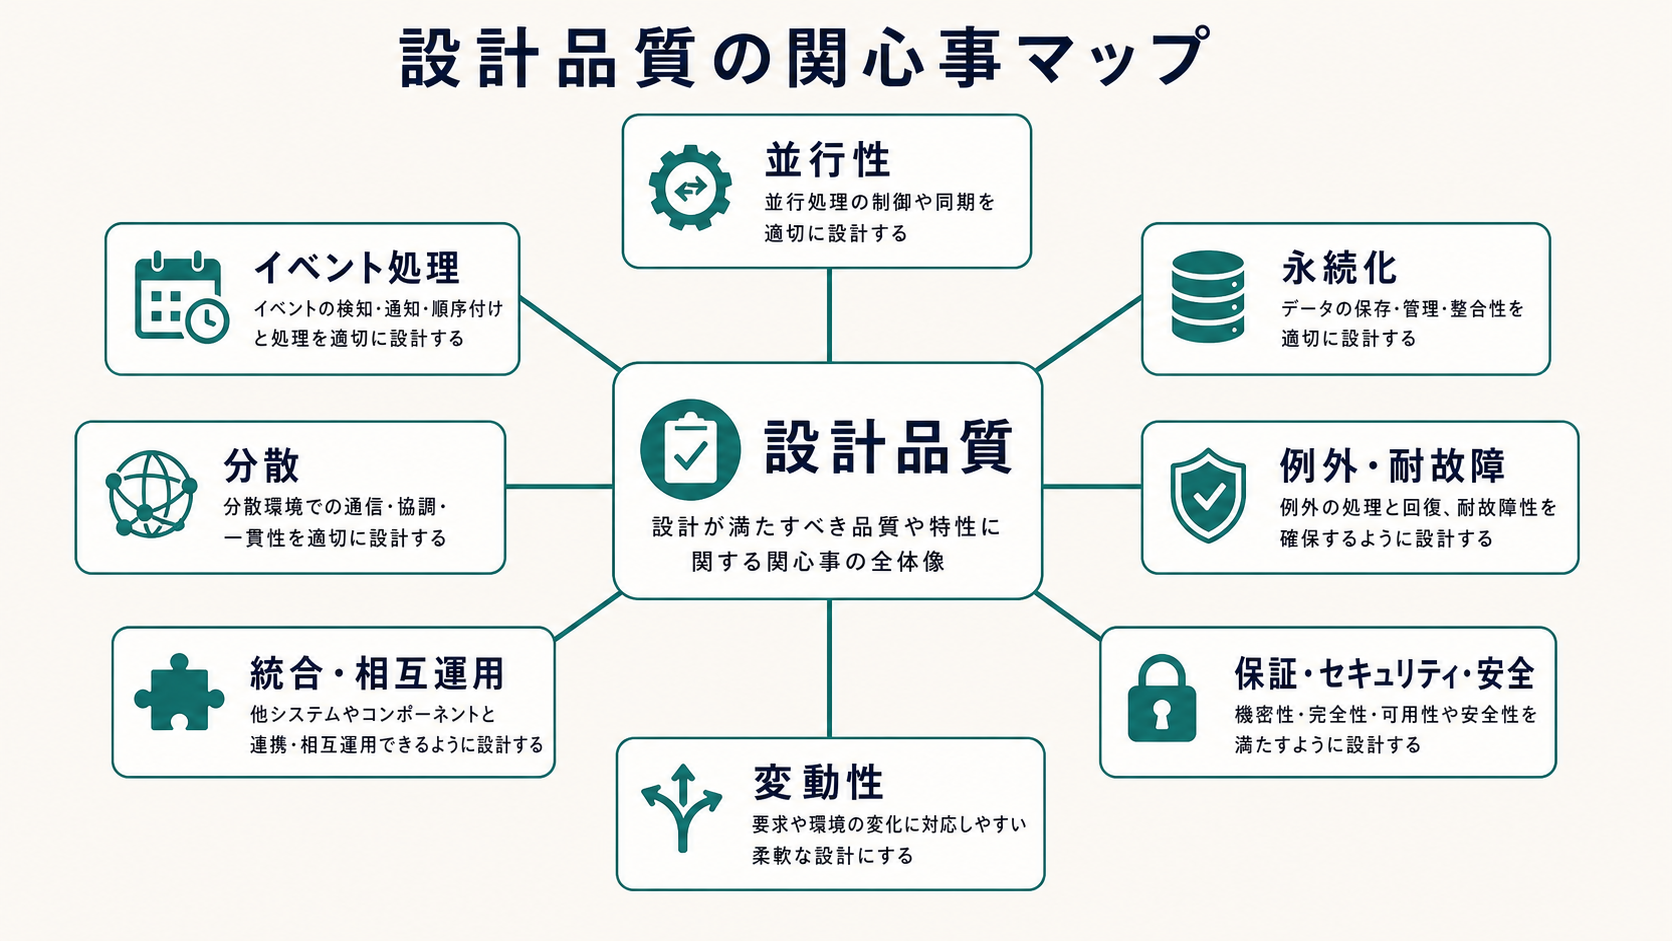
\includegraphics[width=0.96\linewidth]{assets/generated_figures/ch03/fig-ch03-06.png}}{\fbox{\parbox[c][48mm][c]{0.9\linewidth}{\centering 画像生成待ち\\設計品質の関心事マップ}}}
\caption{設計品質の関心事マップ}
\label{fig:ch03-06}
\end{figure}

\subsection{ソフトウェア設計の記録}

設計プロセスの成果は、設計者の頭の中だけに残しておくべきではない。設計記録は、問題、解決策、判断、根拠を関係者へ伝えるためのものである。設計記録には、文章、図、表、モデル、プロトタイプ、コード片などが含まれる。

設計記録の目的は、実装者に作るべきものを示すことだけではない。顧客、テスト担当、品質保証担当、認証担当、保守担当も設計情報を必要とする。したがって、どの設計情報を、誰に向けて、どの詳細度で記録するかを意識して決める必要がある。

\begin{pointbox}{基本方針}
設計記録は「すべてを詳細に書く」ことが目的ではない。読者、利用目的、リスク、保守期間に応じて、必要な設計知識を取り出しやすい形で残すことが目的である。
\end{pointbox}

\subsubsection{モデルに基づく設計}

\term{モデルに基づく設計}{Model-Based Design, MBD} は、モデルを設計記録の中心に置く方法である。従来の文書中心の設計では、自然言語と非形式的な図を使うため、曖昧さや不完全さが残りやすい。また、必要な情報が複数文書に分散し、理解や分析が難しくなる。

モデルに基づく設計では、ツールが設計情報を整理し、表示し、分析できる。たとえば、モデルの一部をアニメーションやシミュレーションで確認したり、仮定を変えた場合の影響を調べたり、要求から設計、設計からテストへの追跡を支援したりできる。

\term{モデル駆動開発}{Model-Driven Development, MDD} は、モデルを開発プロセスの主要成果物として使い、コード生成や検証へつなげる考え方である。

\begin{figure}[htbp]
\centering
\IfFileExists{assets/generated_figures/ch03/fig-ch03-07.png}{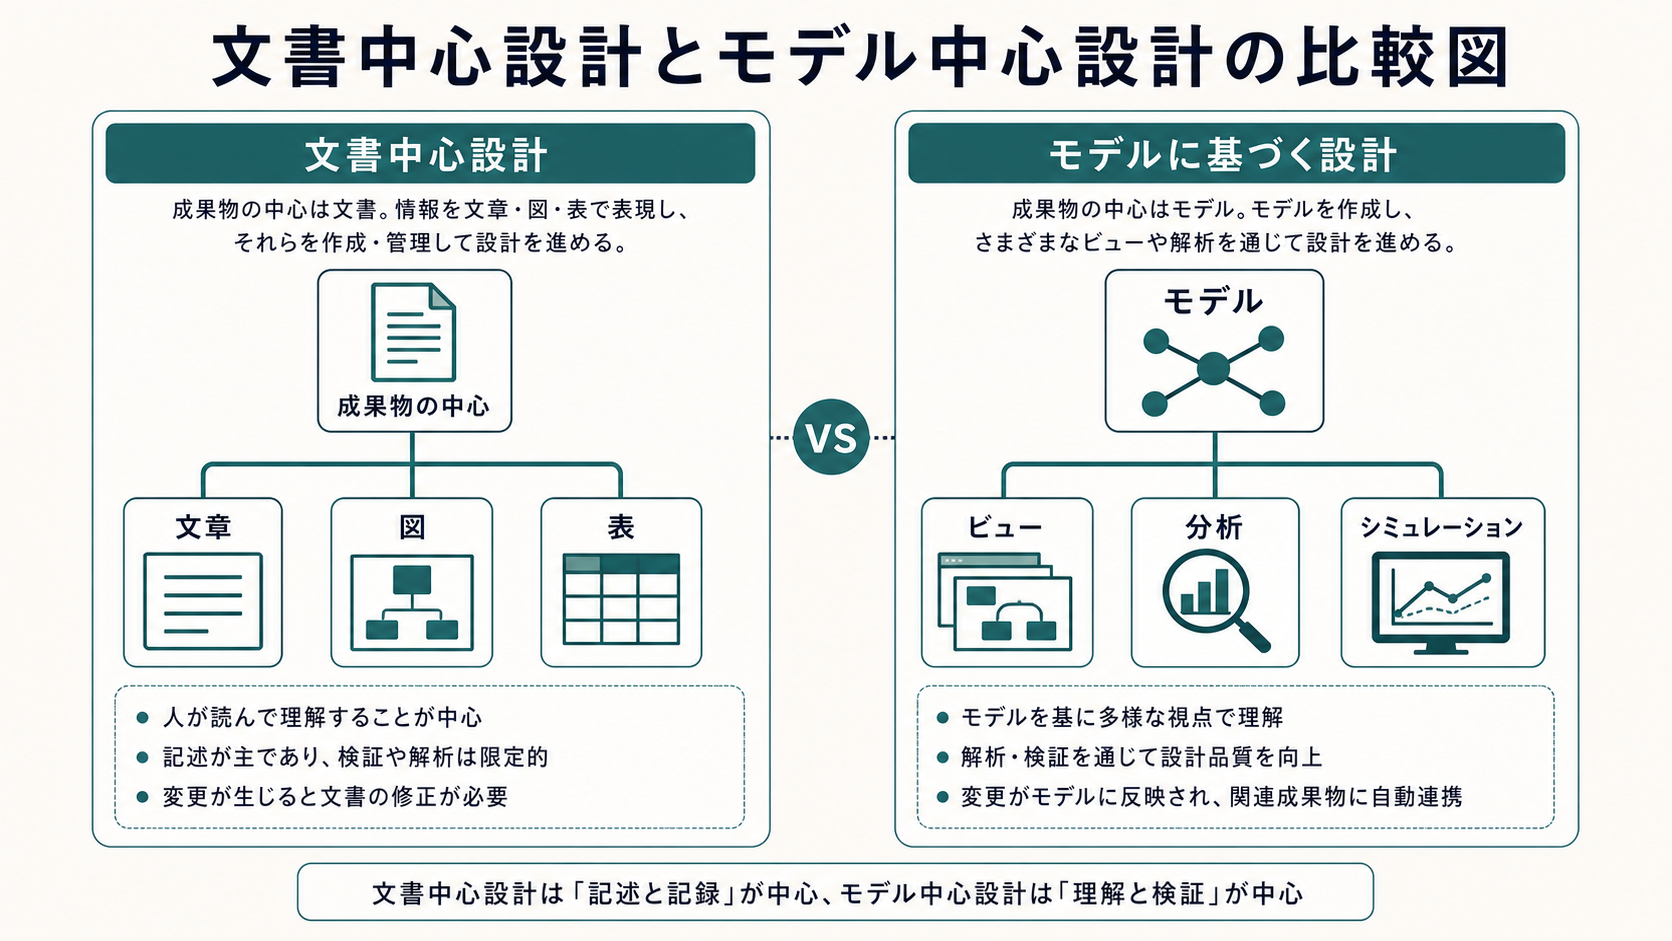
\includegraphics[width=0.96\linewidth]{assets/generated_figures/ch03/fig-ch03-07.png}}{\fbox{\parbox[c][48mm][c]{0.9\linewidth}{\centering 画像生成待ち\\文書中心設計とモデル中心設計の比較図}}}
\caption{文書中心設計とモデル中心設計の比較図}
\label{fig:ch03-07}
\end{figure}

\subsubsection{構造設計記述}

\term{構造設計記述}{Structural Design Description} は、ソフトウェアの静的な構造を表す。つまり、どの構成要素があり、それらがどう関係し、どの責務を持つかを示す。

代表的な記法は次のとおりである。

\par\smallskip\noindent\refstepcounter{table}\label{tab:ch03-04}\textbf{表 \thetable: 第03章 ソフトウェア設計 表04}\par\smallskip
\begin{longtable}{L{42mm}L{112mm}}
\toprule
\textbf{記法} & \textbf{説明} \\
\midrule
\endhead
クラス図・オブジェクト図 & クラス、オブジェクト、属性、操作、関連を表す。オブジェクト指向設計でよく使われる。 \\
コンポーネント図 & 交換可能な構成要素と、その提供・要求インタフェースを表す。 \\
CRCカード & クラス名、責務、協調相手をカード形式で整理する。初期設計や会話に向く。 \\
配置図 & ソフトウェアをどの物理ノードや実行環境へ配置するかを表す。 \\
実体関連図 & データの実体、属性、関係を表す。データ設計でよく使われる。 \\
インタフェース記述言語 & 構成要素が公開する操作名、型、引数、戻り値などを記述する。 \\
構造チャート & プログラムの呼び出し構造を表す。どのモジュールがどのモジュールを呼ぶかを示す。 \\
\bottomrule
\end{longtable}

\subsubsection{振る舞い設計記述}

\term{振る舞い設計記述}{Behavioral Design Description} は、ソフトウェアが時間の中でどのように動くかを表す。処理の流れ、イベントへの反応、状態変化、入力と出力の関係などを示す。

代表的な記法は次のとおりである。

\par\smallskip\noindent\refstepcounter{table}\label{tab:ch03-05}\textbf{表 \thetable: 第03章 ソフトウェア設計 表05}\par\smallskip
\begin{longtable}{L{42mm}L{112mm}}
\toprule
\textbf{記法} & \textbf{説明} \\
\midrule
\endhead
活動図 & 処理の流れ、分岐、並行活動、入力、出力を表す。 \\
相互作用図 & オブジェクトや構成要素間のメッセージ交換を表す。通信図とシーケンス図が代表である。 \\
データフロー図 & 処理要素間を流れるデータを表す。セキュリティ分析にも使える。 \\
決定表・決定図 & 条件の組合せと、それに対応する動作を表す。複雑な業務規則に向く。 \\
フローチャート & 制御の流れと処理順序を表す。 \\
状態遷移図・状態チャート & 状態、イベント、遷移、状態ごとの振る舞いを表す。 \\
形式仕様言語 & 数学的な記法で、インタフェースや振る舞いを厳密に定義する。 \\
擬似コード・プログラム設計言語 & プログラムに近い形で処理手順を表す。詳細設計やアルゴリズム説明に使う。 \\
\bottomrule
\end{longtable}

\begin{figure}[htbp]
\centering
\IfFileExists{assets/generated_figures/ch03/fig-ch03-08.png}{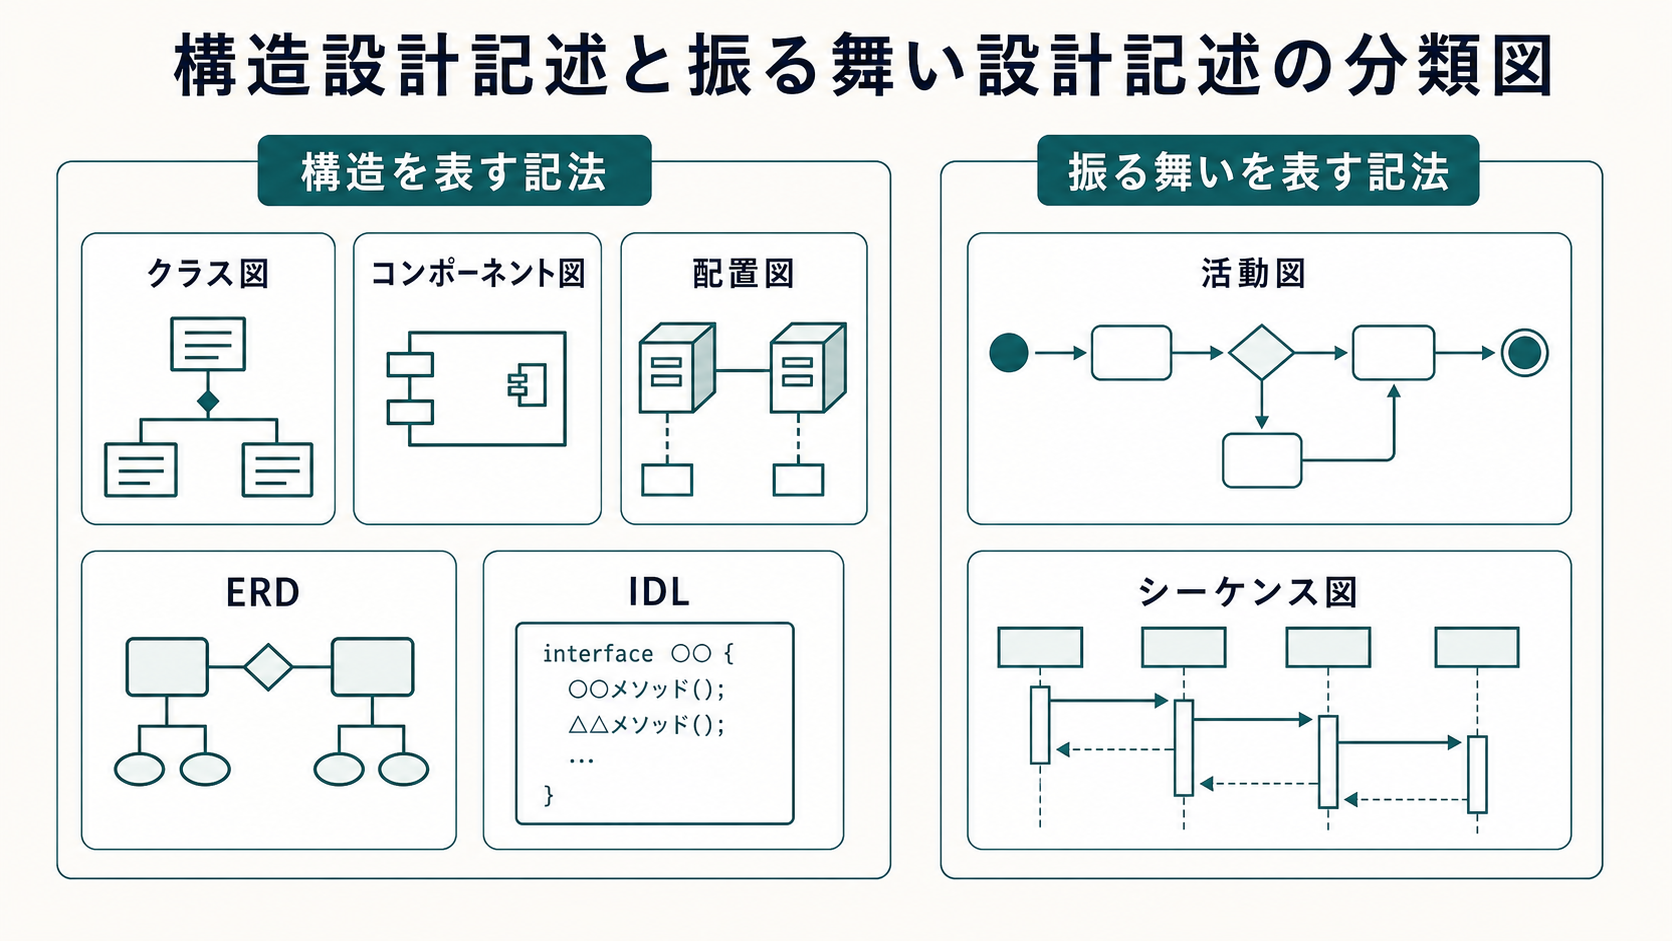
\includegraphics[width=0.96\linewidth]{assets/generated_figures/ch03/fig-ch03-08.png}}{\fbox{\parbox[c][48mm][c]{0.9\linewidth}{\centering 画像生成待ち\\構造設計記述と振る舞い設計記述の分類図}}}
\caption{構造設計記述と振る舞い設計記述の分類図}
\label{fig:ch03-08}
\end{figure}

\subsubsection{設計パターンとスタイル}

\term{設計パターン}{Design Pattern} は、特定の文脈で繰り返し現れる問題に対する一般的な解決策である。設計パターンは、過去に有効だった設計上の慣用句を共有するための語彙である。

代表的な分類は、生成、構造、振る舞いである。
\begin{itemize}
  \item \textbf{生成パターン}：オブジェクトや部品の生成方法を扱う。ビルダー、ファクトリ、プロトタイプ、シングルトンなどがある。
  \item \textbf{構造パターン}：部品の組み合わせ方を扱う。アダプタ、ブリッジ、コンポジット、デコレータ、ファサード、プロキシなどがある。
  \item \textbf{振る舞いパターン}：責務の分担や相互作用を扱う。コマンド、イテレータ、メディエータ、オブザーバ、状態、戦略、テンプレート、ビジタなどがある。
\end{itemize}

\term{スタイル}{Style} は、より大きな構造の特徴を表す場合に使われることが多い。たとえば、階層化、パイプ・アンド・フィルタ、クライアントサーバ、イベント駆動などは、システム全体または大きな部分の設計方針として現れる。

\begin{figure}[htbp]
\centering
\IfFileExists{assets/generated_figures/ch03/fig-ch03-09.png}{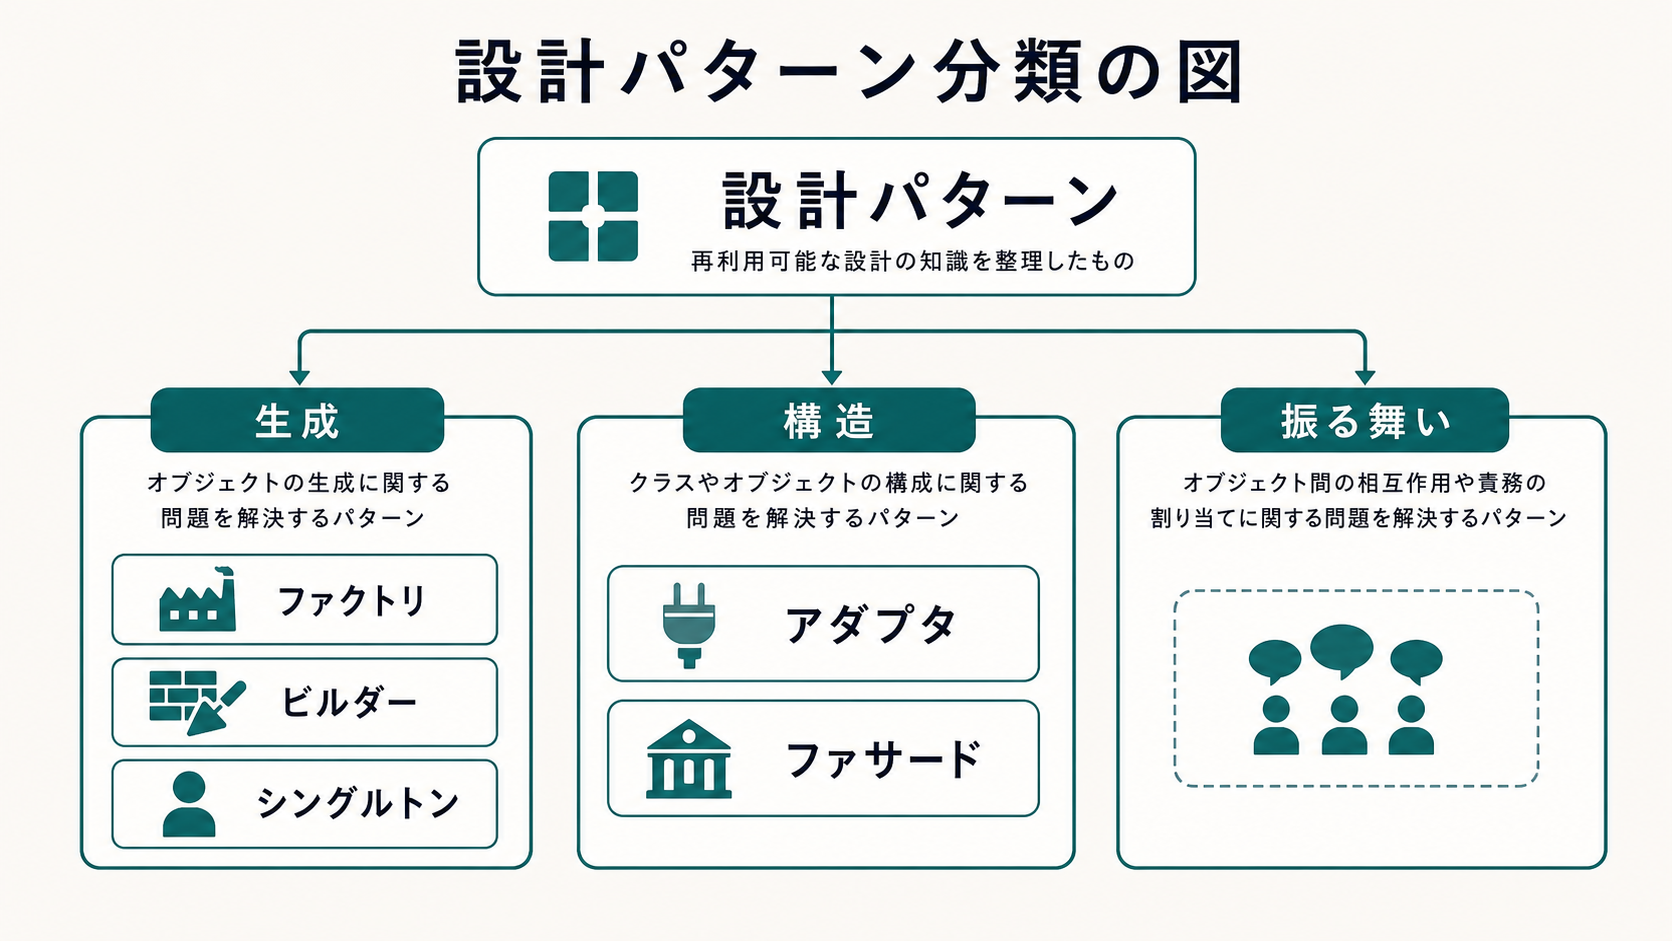
\includegraphics[width=0.96\linewidth]{assets/generated_figures/ch03/fig-ch03-09.png}}{\fbox{\parbox[c][48mm][c]{0.9\linewidth}{\centering 画像生成待ち\\設計パターン分類の図}}}
\caption{設計パターン分類の図}
\label{fig:ch03-09}
\end{figure}

\subsubsection{専用言語と領域固有言語}

設計表現は、構造と振る舞いの二分法だけで整理できるとは限らない。たとえば、利用者インタフェース設計では、画面の構造、操作の流れ、入力制約、表示規則が混ざる。また、安全性や信頼性の領域では、その分野に特化した記法が発達している。

\term{領域固有言語}{Domain-Specific Language, DSL} は、特定の業務領域や技術領域の概念を直接表すための言語である。汎用プログラミング言語ではなく、その領域の語彙を使って設計や実装に近い表現を行う。例として、シミュレーション、リアルタイムシステム、ゲーム開発、利用者インタフェース、テスト開発、言語処理などの領域向けDSLがある。

DSLの利点は、領域の専門家が理解しやすい語彙で表現できることである。一方、DSLを作るには、言語仕様、構文解析、生成、保守の負担がある。したがって、繰り返し使う価値がある領域で特に有効である。

\subsubsection{設計根拠}

\term{設計根拠}{Design Rationale} は、なぜその設計判断をしたかを説明する情報である。設計根拠には、前提、検討した代替案、採用基準、トレードオフ、却下した案の理由が含まれる。

設計チームにとって、現在の判断理由は明らかに見えることが多い。しかし、数か月後、数年後、または担当者交代後には、その理由が失われる。設計根拠を記録すれば、保守担当者は「なぜこの構造なのか」「なぜ別案を採らなかったのか」を理解しやすい。

却下した判断を記録することも有用である。前提や制約が変わったとき、以前は却下された案が有効になる場合がある。逆に、過去に明確な理由で却下された案を、理由を忘れて再び採用してしまうことを防げる。

\begin{pointbox}{実務の見方}
設計根拠は、巨大な説明文である必要はない。「判断」「理由」「代替案」「影響」「未解決事項」を短く残すだけでも、後の保守で大きな価値を持つ。
\end{pointbox}

\subsection{ソフトウェア設計戦略と方法}

設計戦略と方法は、設計プロセスを進めるための考え方である。方法によって、何を最初に見るか、どのように分解するか、どの概念を中心に置くかが異なる。

\subsubsection{一般戦略}

一般的な設計戦略には、分割統治、段階的詳細化、トップダウン、ボトムアップ、反復、増分、パターン利用などがある。

\term{分割統治}{divide and conquer} は、大きな問題を小さな問題に分けて解く考え方である。\term{段階的詳細化}{stepwise refinement} は、粗い設計から始め、徐々に詳細を追加する考え方である。トップダウンは全体から部分へ進む。ボトムアップは既存部品や低水準機能から全体を組み立てる。

実務では、これらは単独で使われるというより、組み合わせて使われる。最初にトップダウンで全体構造を作り、既存部品をボトムアップで組み込み、反復しながら詳細化することが多い。

\subsubsection{機能指向・構造化設計}

\term{機能指向設計}{Function-Oriented Design} または\term{構造化設計}{Structured Design} は、ソフトウェアの主要機能を見つけ、それを上位から下位へ分解する古典的な方法である。

この方法では、データフロー図や処理記述を使い、入力がどの処理を通って出力へ変換されるかを考える。業務処理の流れが明確で、機能分解しやすいシステムで理解しやすい。一方、状態やデータ構造、イベント、オブジェクト間の相互作用が複雑な場合は、別の方法と組み合わせる必要がある。

\subsubsection{データ中心設計}

\term{データ中心設計}{Data-Centered Design} は、プログラムが扱うデータ構造から設計を始める方法である。入力データ構造と出力データ構造を明らかにし、入力を出力へ変換する処理単位を設計する。

データが安定しており、処理がデータ構造に強く依存する場合に有効である。たとえば、ファイル変換、帳票生成、データ処理パイプラインなどでは、データ構造を中心に考えると設計しやすい。

\subsubsection{オブジェクト指向設計}

\term{オブジェクト指向設計}{Object-Oriented Design} は、オブジェクトを中心に設計する方法である。オブジェクトは、データと操作を一体として持つ概念である。設計では、クラス、属性、メソッド、関連、継承、多態性、責務を考える。

初期のオブジェクト指向設計では、名詞からオブジェクトを見つけ、動詞からメソッドを見つける方法が使われた。現在では、単に名詞を拾うだけでなく、責務を中心に設計する考え方が重要である。クラスが何を知り、何を行い、誰と協調するかを考える。

SOLID原則は、クラス設計でよく参照される考え方である。単一責任、開放閉鎖、リスコフ置換、インタフェース分離、依存関係逆転の頭文字である。これらは、変更しやすく理解しやすいオブジェクト指向設計を目指すための指針である。

\subsubsection{利用者中心設計}

\term{利用者中心設計}{User-Centered Design} は、利用者とその作業、目的、文脈を深く理解したうえで設計する方法である。単に画面をきれいにすることではなく、利用者が何を達成したいか、どのような環境で使うか、どのような誤りを起こしやすいかを考える。

利用者中心設計では、利用者要求の収集、作業の流れの整理、プロトタイプやモックアップの作成、利用者評価を行う。使いやすさが重要なシステムでは、利用者中心設計を後から追加するのではなく、設計の初期から組み込む必要がある。

\subsubsection{構成要素ベース設計}

\term{構成要素ベース設計}{Component-Based Design, CBD} は、独立して配置・利用できる構成要素を組み合わせてシステムを作る方法である。各構成要素は、明確なインタフェースと依存関係を持つ。

この方法の目的は、再利用、独立開発、交換容易性、統合容易性を高めることである。構成要素ベース設計では、共通API、サービスごとのAPI、部品のバージョン、依存関係、配置方法が重要になる。

\subsubsection{イベント駆動設計}

\term{イベント駆動設計}{Event-Driven Design} は、イベントに反応して処理を行う設計方法である。イベントとは、利用者操作、メッセージ受信、状態変化、タイマー発火、センサー入力などである。

イベント駆動設計では、発行・購読方式がよく使われる。送信側はイベントを発行し、受信側は関心のあるイベントを購読する。これにより、送信側と受信側の結合を弱められる。大規模で拡張性が必要なシステムでは有効だが、イベントの順序、重複、遅延、失敗時の影響を慎重に設計する必要がある。

\subsubsection{アスペクト指向設計}

\term{アスペクト指向設計}{Aspect-Oriented Design, AOD} は、横断的関心事をアスペクトとして分離する方法である。横断的関心事とは、ログ、セキュリティ確認、トランザクション、例外処理など、複数の機能にまたがる関心である。

アスペクト指向の考え方は、必ずしも独立した設計手法として広く使われているわけではない。しかし、アプリケーションフレームワークやライブラリでは、宣言や設定によって横断的な振る舞いを追加する形で利用されることがある。

\subsubsection{制約に基づく設計}

\term{制約に基づく設計}{Constraint-Based Design} は、制約を使って設計空間を狭める方法である。設計空間とは、可能な設計案全体の集合である。制約は、不可能または受け入れられない案を除外する役割を持つ。

制約には、ハードウェア、ソフトウェア、データ、操作手順、インタフェース、法令、性能、費用、納期などが含まれる。制約を明確にすれば、設計探索が速くなる。一方、制約が多すぎる場合や互いに矛盾する場合は、解が見つからないこともある。

\subsubsection{ドメイン駆動設計}

\term{ドメイン駆動設計}{Domain-Driven Design} は、対象領域の概念と言葉を中心に設計する方法である。ここでいうドメインとは、銀行、医療、物流、教育、ゲームなど、ソフトウェアが扱う問題領域である。

ドメイン駆動設計では、分析者、設計者、開発者、業務専門家が共有する言葉を重視する。この共有語彙を使って、オブジェクト、役割、イベント、活動、規則を設計記述に反映する。言葉がずれると、実装もずれるため、ドメインの語彙を設計の中心に置くことが重要である。

\subsubsection{その他の方法}

その他にも、多くの設計方法がある。反復型・適応型の方法では、厳密な要求と設計を最初にすべて固定するのではなく、ソフトウェア増分を作りながら設計を調整する。

\term{サービス指向設計}{Service-Oriented Design} は、分散されたサービスを組み合わせてソフトウェアを作る方法である。HTTP、HTTPS、SOAPなどの標準プロトコルを使い、異なる提供者のサービスをつなぐことがある。

\begin{figure}[htbp]
\centering
\IfFileExists{assets/generated_figures/ch03/fig-ch03-10.png}{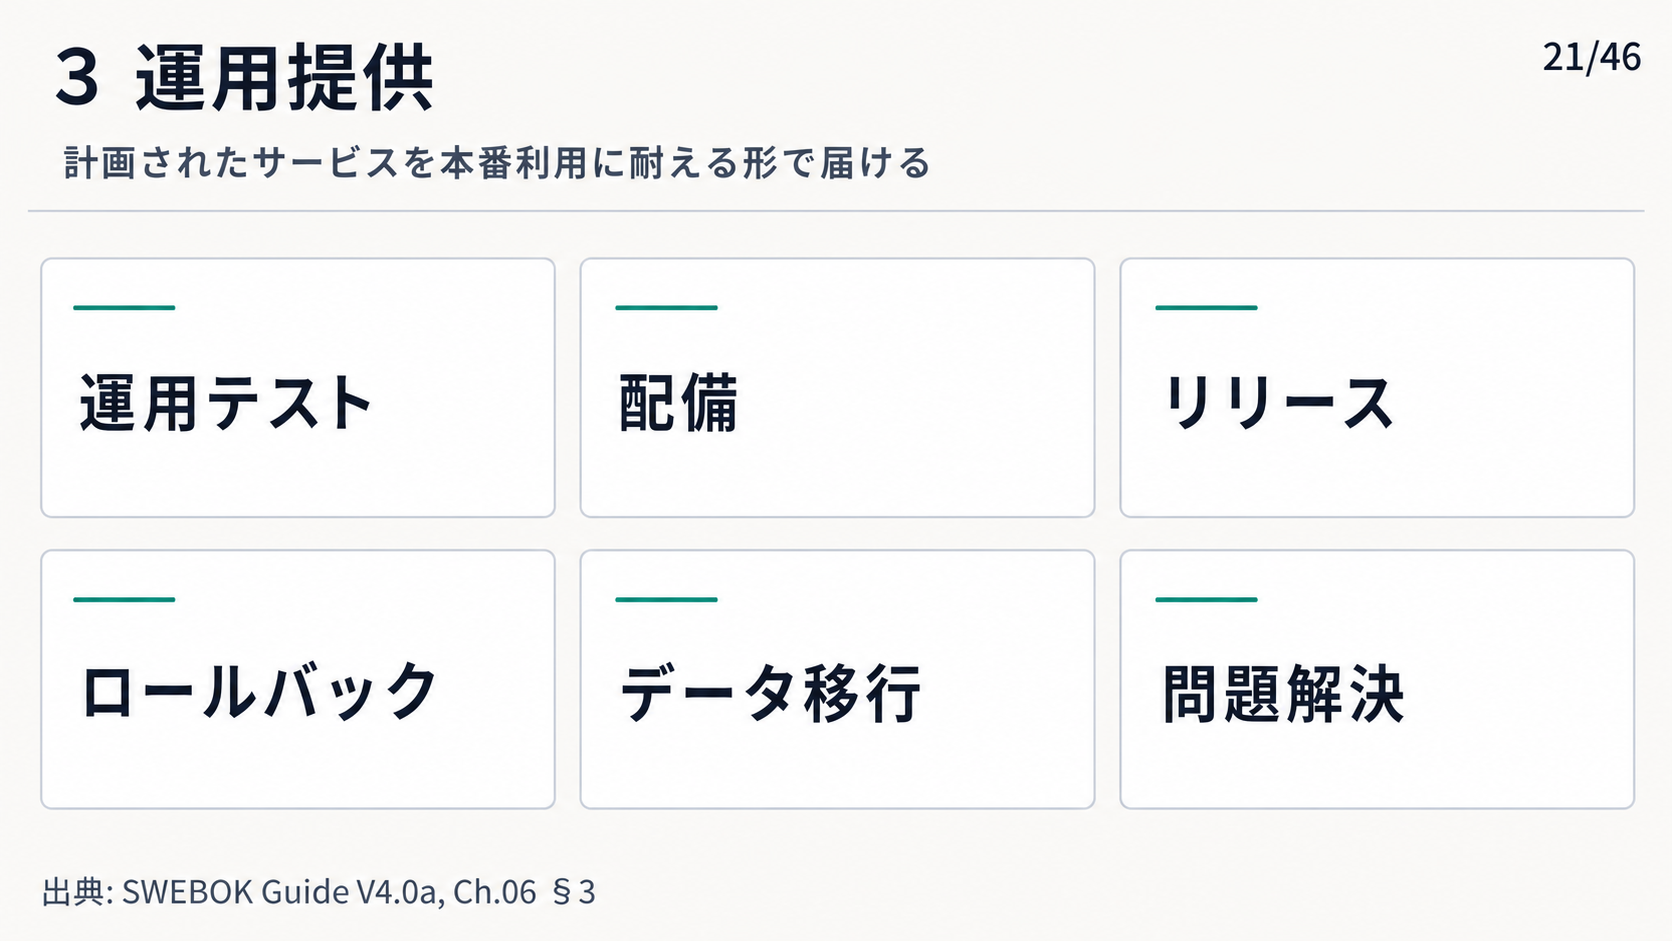
\includegraphics[width=0.96\linewidth]{assets/generated_figures/ch03/fig-ch03-10.png}}{\fbox{\parbox[c][48mm][c]{0.9\linewidth}{\centering 画像生成待ち\\設計戦略と中心概念の対応図}}}
\caption{設計戦略と中心概念の対応図}
\label{fig:ch03-10}
\end{figure}

\subsection{ソフトウェア設計品質分析と評価}

設計は、作ったら終わりではない。設計が要求を満たすか、品質属性を達成できるか、保守しやすいか、リスクが残っていないかを分析・評価する必要がある。

\subsubsection{設計レビューと監査}

\term{設計レビュー}{Design Review} は、設計を包括的に調べる活動である。目的は、設計の完成度、要求の網羅、未解決事項、潜在問題、品質リスクを確認することである。レビューは、設計チーム自身、独立した第三者、顧客、品質保証担当などによって行われる。

\term{設計監査}{Design Audit} は、より狭い観点に焦点を当てる。たとえば、特定の機能監査、標準への適合監査、セキュリティ方針への適合監査などである。

\begin{figure}[htbp]
\centering
\IfFileExists{assets/generated_figures/ch03/fig-ch03-11.png}{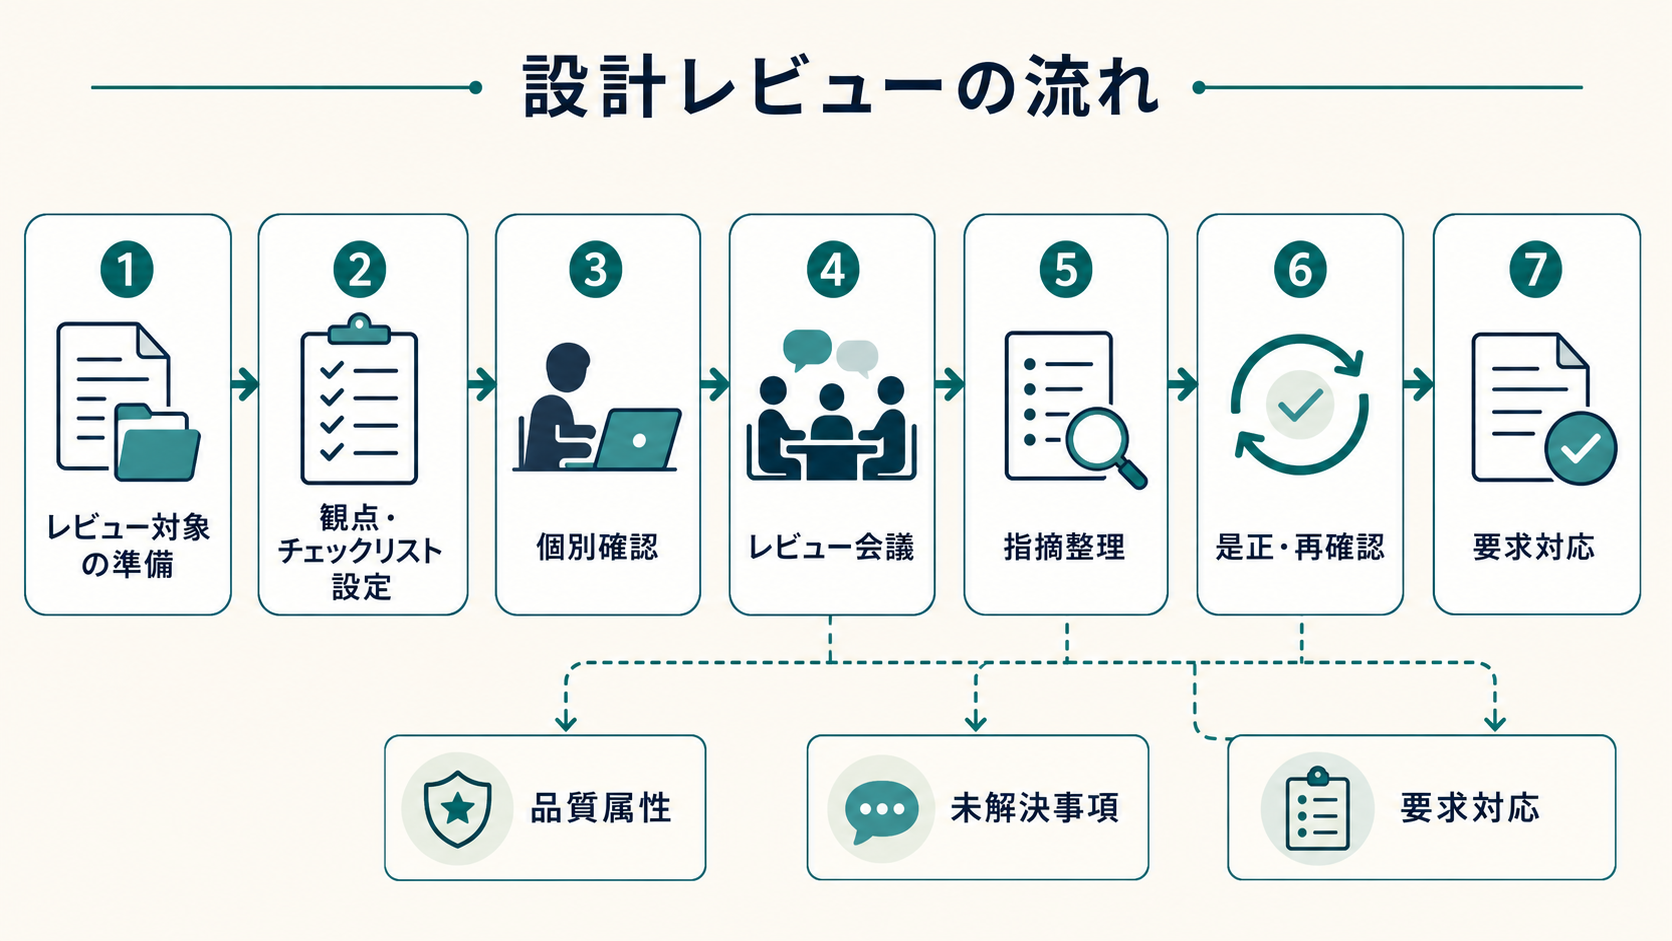
\includegraphics[width=0.96\linewidth]{assets/generated_figures/ch03/fig-ch03-11.png}}{\fbox{\parbox[c][48mm][c]{0.9\linewidth}{\centering 画像生成待ち\\設計レビューの流れ}}}
\caption{設計レビューの流れ}
\label{fig:ch03-11}
\end{figure}

\subsubsection{品質属性}

設計品質に関わる属性には、モジュール性、保守容易性、移植性、テスト容易性、使いやすさ、正しさ、堅ろう性などがある。これらは、利害関係者の関心事の大きな部分を占める。

品質属性には、実行時に観察できるものと、実行時には直接見えにくいものがある。性能、セキュリティ、可用性、機能性、使いやすさは、実行時に観察しやすい。一方、変更容易性、移植性、再利用性、テスト容易性は、設計や保守の中で評価されることが多い。概念的一貫性、正しさ、完全性は、設計記述そのものを見て評価される。

\subsubsection{品質分析・評価技法}

設計品質を分析・評価するための技法には、静的分析、シミュレーション、プロトタイピング、レビュー、要求追跡などがある。

\par\smallskip\noindent\refstepcounter{table}\label{tab:ch03-06}\textbf{表 \thetable: 第03章 ソフトウェア設計 表06}\par\smallskip
\begin{tabularx}{\linewidth}{L{36mm}Y}
\toprule
\textbf{技法} & \textbf{説明} \\
\midrule
設計レビュー・検査 & 設計記述を人が確認し、要求対応、未解決事項、設計上のリスクを見つける。 \\
シナリオに基づく評価 & 利用シナリオ、障害シナリオ、変更シナリオを使って、設計がどう反応するか確認する。 \\
要求追跡 & 要求が設計要素へ対応しているか、設計要素に根拠となる要求があるか確認する。 \\
静的分析 & 実行せずに設計やモデルを分析する。依存関係、循環、整合性、弱点を確認する。 \\
形式的分析 & 数学的モデルを使い、性質を厳密に検査する。安全性やセキュリティが重要な領域で有効である。 \\
シミュレーション & 設計モデルを使い、性能、タイミング、負荷、失敗時の挙動などを試す。 \\
プロトタイピング & 実現可能性、使いやすさ、技術的リスクを確認するために試作品を作る。 \\
\bottomrule
\end{tabularx}

\begin{figure}[htbp]
\centering
\IfFileExists{assets/generated_figures/ch03/fig-ch03-12.png}{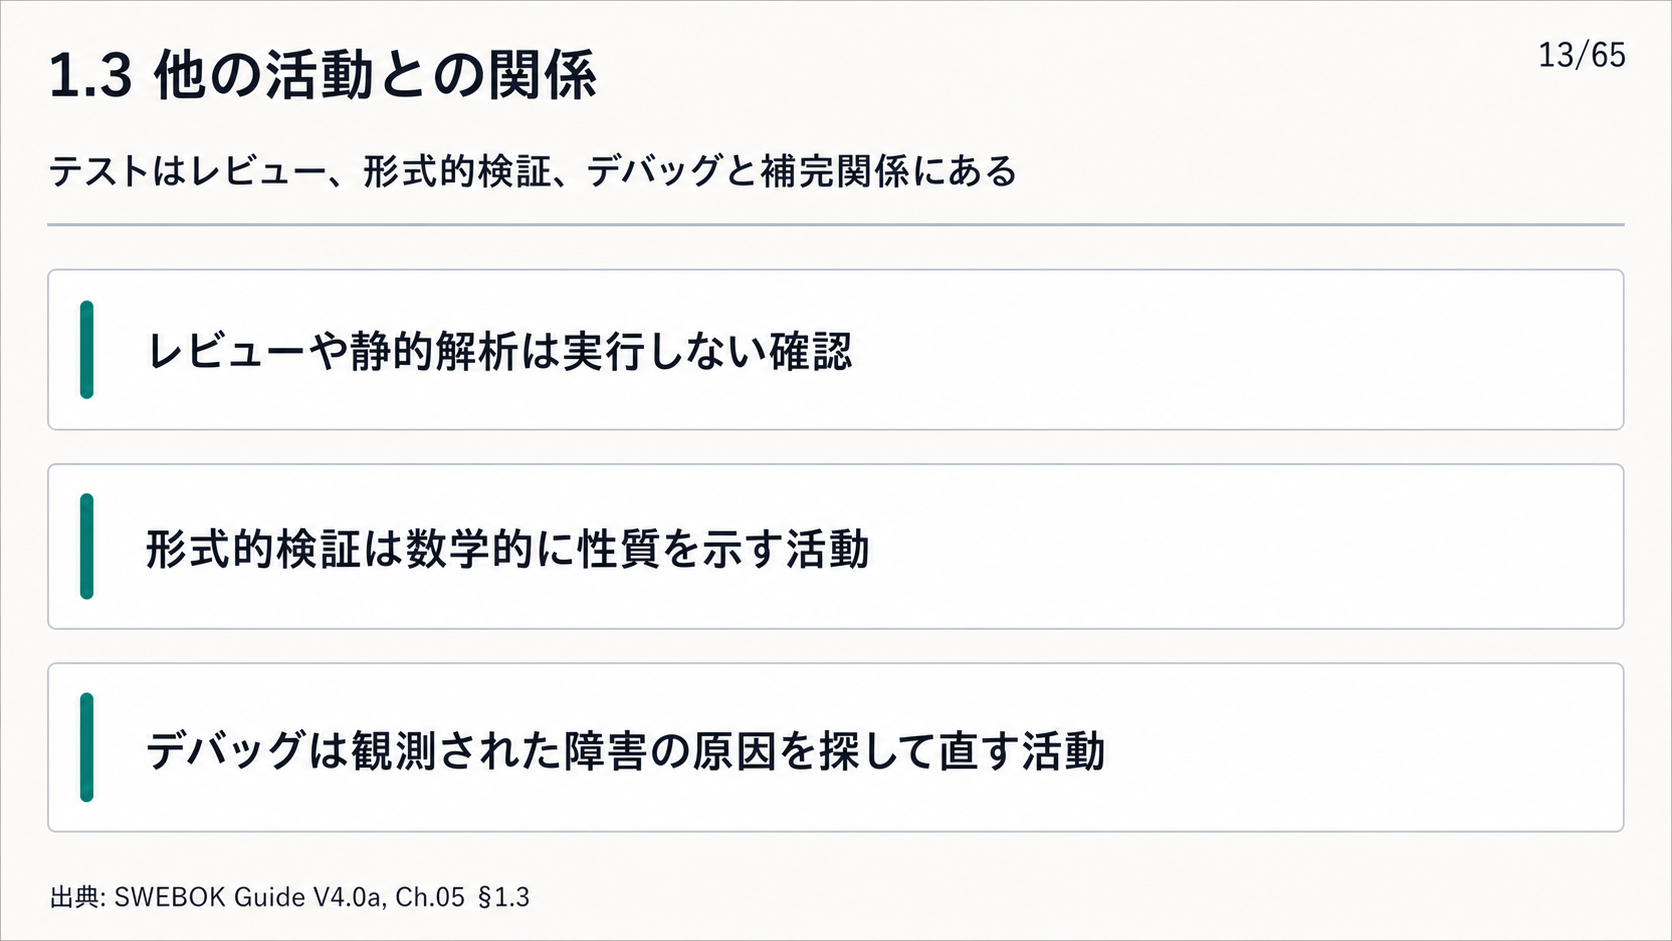
\includegraphics[width=0.96\linewidth]{assets/generated_figures/ch03/fig-ch03-12.png}}{\fbox{\parbox[c][48mm][c]{0.9\linewidth}{\centering 画像生成待ち\\品質分析・評価技法の比較図}}}
\caption{品質分析・評価技法の比較図}
\label{fig:ch03-12}
\end{figure}

\subsubsection{測度とメトリクス}

\term{測度}{Measure} と\term{メトリクス}{Metric} は、設計の大きさ、構造、複雑さ、品質を定量的に見るために使われる。測定対象は、設計方法によって異なる。

機能分解を中心とする設計では、構造チャートなどから、階層の深さ、モジュール数、呼び出し関係の複雑さを測る。オブジェクト指向設計では、クラス図などから、クラス数、継承の深さ、結合度、凝集度、メソッド数、メッセージ数などを測る。

測度は、設計の良し悪しを自動的に決めるものではない。測度は、注意すべき箇所を見つける手がかりである。たとえば、結合度が高い部品は変更の影響が大きい可能性がある。凝集度が低い部品は責務が散らばっている可能性がある。

\subsubsection{検証・妥当性確認・認証}

設計の分析と評価は、検証、妥当性確認、認証に関わる。

\par\smallskip\noindent\refstepcounter{table}\label{tab:ch03-07}\textbf{表 \thetable: 第03章 ソフトウェア設計 表07}\par\smallskip
\begin{tabularx}{\linewidth}{L{32mm}Y}
\toprule
\textbf{活動} & \textbf{意味} \\
\midrule
検証 & 設計が、明示された要求を満たしているかを確認することである。 \\
妥当性確認 & その設計で作られるシステムが、顧客、利用者、運用者、保守担当者の期待を満たせるかを確認することである。 \\
認証 & 第三者が、設計が仕様や意図された利用に適合していると証明または表明することである。 \\
\bottomrule
\end{tabularx}

検証は「要求どおりか」を問う。妥当性確認は「本当に役に立つか」を問う。認証は「決められた基準に適合していると第三者が認めるか」を問う。安全性や規制が重要な領域では、設計段階から認証を見据えた証拠を残す必要がある。

\subsection{トピックと参考文献の対応}

この表は、SWEBOKが示す「トピック対参考資料の行列」を、学習用に簡略化したものである。詳しく学ぶときは、各トピックに対応する文献を読む。

\par\smallskip\noindent\refstepcounter{table}\label{tab:ch03-08}\textbf{表 \thetable: 第03章 ソフトウェア設計 表08}\par\smallskip
\begin{longtable}{L{66mm}L{98mm}}
\toprule
\textbf{トピック} & \textbf{主な参考資料} \\
\midrule
\endhead
1. ソフトウェア設計の基礎 & Brooks, The Design of Design; Budgen, Software Design \\
1.1 設計思考 & Brooks; Budgen; Ross, Goodenough and Irvine \\
1.2 ソフトウェア設計の文脈 & Budgen; Sommerville \\
1.3 ソフトウェア設計の主要論点 & Brooks; Budgen; Sommerville; Bosch \\
1.4 ソフトウェア設計原則 & Budgen; Dijkstra; Parnas; ISO/IEC/IEEE 24765; IEEE Std 7000 \\
2. ソフトウェア設計プロセス & Budgen; Sommerville; ISO/IEC/IEEE 12207 \\
2.1 高水準設計 & Brooks; Budgen \\
2.2 詳細設計 & Budgen; Sommerville \\
3. ソフトウェア設計品質 & Budgen; Sommerville; Galster et al. \\
3.1 並行性 & Sommerville \\
3.2 制御とイベント処理 & Sommerville; Luckham; Mühl, Fiege and Pietzuch \\
3.3 データ永続化 & Sommerville \\
3.4 構成要素の分散 & Sommerville \\
3.5 誤り・例外処理と耐故障性 & Sommerville \\
3.6 統合と相互運用性 & Budgen \\
3.7 保証・セキュリティ・安全性 & Sommerville \\
3.8 変動性 & Galster et al.; Bosch \\
4. ソフトウェア設計の記録 & Booch, Rumbaugh and Jacobson; Budgen; Sommerville \\
4.1 モデルに基づく設計 & Budgen; Sommerville \\
4.2 構造設計記述 & Booch et al.; Budgen; Gamma et al.; Sommerville \\
4.3 振る舞い設計記述 & Booch et al.; Budgen; Gamma et al.; Sommerville \\
4.4 設計パターンとスタイル & Brooks; Budgen; Gamma et al.; Sommerville \\
4.5 専用言語と領域固有言語 & Sommerville; Kosar, Bohra and Mernik \\
4.6 設計根拠 & Brooks; Budgen; Sommerville; Parnas and Clements \\
5. ソフトウェア設計戦略と方法 & Sommerville; Budgen; Nielsen; Kiczales et al. \\
5.1 一般戦略 & Budgen \\
5.2 機能指向・構造化設計 & Budgen \\
5.3 データ中心設計 & Budgen; Sommerville \\
5.4 オブジェクト指向設計 & Budgen; Booch et al. \\
5.5 利用者中心設計 & Brooks; Nielsen \\
5.6 構成要素ベース設計 & Booch et al.; Budgen; Sommerville \\
5.7 イベント駆動設計 & Sommerville; Luckham; Mühl et al. \\
5.8 アスペクト指向設計 & Booch et al.; Sommerville; Kiczales et al. \\
5.9 制約に基づく設計 & Brooks \\
5.10 ドメイン駆動設計 & Budgen \\
5.11 その他の方法 & Sommerville \\
6. 設計品質分析と評価 & Budgen; Sommerville; Parnas and Weiss \\
6.1 設計レビューと監査 & Budgen; Parnas and Weiss \\
6.2 品質属性 & Sommerville \\
6.3 品質分析・評価技法 & Sommerville; Software Quality KA \\
6.4 測度とメトリクス & Budgen; Sommerville \\
6.5 検証・妥当性確認・認証 & Sommerville; Software Quality KA \\
\bottomrule
\end{longtable}

\subsection{発展的な読み物}

SWEBOK 03章で紹介される発展的な読み物を、日本語で読む目的に合わせて整理する。

\par\smallskip\noindent\refstepcounter{table}\label{tab:ch03-09}\textbf{表 \thetable: 第03章 ソフトウェア設計 表09}\par\smallskip
\begin{tabularx}{\linewidth}{L{52mm}Y}
\toprule
\textbf{文献} & \textbf{読むと得られること} \\
\midrule
Brooks, \textit{The Design of Design} & ソフトウェア工学の先駆者による設計論である。設計活動、設計判断、事例を広く学べる。 \\
Budgen, \textit{Software Design} & ソフトウェア設計を体系的に学ぶための中心的な教科書である。構造、振る舞い、設計方法、評価を幅広く扱う。 \\
Gamma et al., \textit{Design Patterns} & 再利用可能なオブジェクト指向設計パターンの古典である。設計語彙を学ぶのに有効である。 \\
Booch, Rumbaugh and Jacobson, \textit{The Unified Modeling Language User Guide} & UMLを使った構造・振る舞いの表現を学べる。設計記述の記法を理解するのに役立つ。 \\
Sommerville, \textit{Software Engineering} & 設計だけでなく、要求、実装、テスト、品質、分散システムなどを含むソフトウェア工学全体を学べる。 \\
Parnas, “On the Criteria To Be Used In Decomposing Systems Into Modules” & モジュール分解と情報隠蔽の古典的論文である。設計原則の背景を学べる。 \\
IEEE Std 7000-2021 & 倫理的関心をシステム設計で扱うための標準である。AIや自律システムの設計で参考になる。 \\
\bottomrule
\end{tabularx}

\subsection{参考文献}

\begin{enumerate}
  \item G. Booch, J. Rumbaugh, and I. Jacobson, \textit{The Unified Modeling Language User Guide}, 2nd edition, Addison-Wesley, 2005.
  \item J. Bosch, \textit{Design and Use of Software Architectures: Adopting and Evolving a Product-Line Approach}, ACM Press, 2000.
  \item F. Brooks, \textit{The Design of Design}, Addison-Wesley, 2010.
  \item D. Budgen, \textit{Software Design: Creating Solutions for Ill-Structured Problems}, 3rd edition, CRC Press, 2021.
  \item E. W. Dijkstra, “On the Role of Scientific Thought,” 1974.
  \item M. Galster, D. Weyns, D. Tofan, B. Michalik, and P. Avgeriou, “Variability in Software Systems - A Systematic Literature Review,” \textit{IEEE Transactions on Software Engineering}, 40(3), 2014.
  \item E. Gamma et al., \textit{Design Patterns: Elements of Reusable Object-Oriented Software}, Addison-Wesley, 1994.
  \item S. Gregor and D. Jones, “The Anatomy of a Design Theory,” Association for Information Systems, 2007.
  \item IEEE Std 7000-2021, \textit{IEEE Standard Model Process for Addressing Ethical Concerns during System Design}.
  \item ISO/IEC/IEEE 12207, \textit{Systems and Software Engineering - Software Life Cycle Processes}.
  \item ISO/IEC/IEEE 24765:2017, \textit{Systems and Software Engineering - Vocabulary}, 2nd ed., 2017.
  \item G. Kiczales et al., “Aspect-Oriented Programming,” Proc. 11th European Conf. Object-Oriented Programming, Springer, 1997.
  \item T. Kosar, S. Bohra, and M. Mernik, “Domain-Specific Languages: A Systematic Mapping Study,” \textit{Information and Software Technology}, 71, 77-91, 2016.
  \item D. Luckham, \textit{The Power of Events: an Introduction to Complex Event Processing}, Addison-Wesley, 2002.
  \item G. Mühl, L. Fiege, and P. Pietzuch, \textit{Distributed Event-Based Systems}, Springer-Verlag, 2006.
  \item J. Nielsen, \textit{Usability Engineering}, Morgan Kaufmann, 1994.
  \item D. L. Parnas, “On the Criteria To Be Used In Decomposing Systems Into Modules,” \textit{Communications of the ACM}, 15(12), 1053-1058, 1972.
  \item D. L. Parnas and P. C. Clements, “A Rational Design Process: How and Why to fake it,” \textit{IEEE Transactions on Software Engineering}, 12(2), 251-257, 1986.
  \item D. L. Parnas and D. M. Weiss, “Active Design Reviews: Principles and Practices,” \textit{Journal of Systems and Software}, 7, 259-265, 1987.
  \item D. T. Ross, J. B. Goodenough, and A. Irvine, “Software Engineering: Process, Principles, and Goals,” \textit{IEEE Computer}, May 1975.
  \item I. Sommerville, \textit{Software Engineering}, 10th edition, Pearson, 2016.
\end{enumerate}

\subsection{章末確認問題}

\begin{enumerate}
  \item ソフトウェア設計という語が持つ四つの意味を説明せよ。
  \item 設計思考の五段階を、自分の言葉で説明せよ。
  \item 高水準設計と詳細設計の違いを、外部向き・内部向きという観点から説明せよ。
  \item 抽象化、モジュール化、カプセル化の違いを説明せよ。
  \item 結合度を低くし、凝集度を高くすることが望ましい理由を説明せよ。
  \item 並行性を設計するとき、同期や排他制御が必要になる理由を説明せよ。
  \item 構造設計記述と振る舞い設計記述の例を、それぞれ三つ挙げよ。
  \item 設計パターンが「語彙」として役立つ理由を説明せよ。
  \item ドメイン駆動設計で、共有語彙が重要になる理由を説明せよ。
  \item 設計レビュー、静的分析、プロトタイピングはどのように使い分けるか。
\end{enumerate}

\begin{pointbox}{解答の方向性}
1は「分野、プロセス、結果、ライフサイクル段階」である。3は、高水準設計が外部とのやり取りや主要構成要素の責務を扱い、詳細設計が内部モジュール、データ構造、アルゴリズムを扱う点を説明する。5は、変更影響の局所化と理解容易性を軸に説明できる。7は、構造ならクラス図、コンポーネント図、ERD、配置図など、振る舞いなら活動図、シーケンス図、DFD、状態遷移図、決定表などを挙げればよい。
\end{pointbox}

\section{第04章 ソフトウェア構築}
\noindent\textbf{この資料の主張}

ソフトウェア構築は、単にプログラムを書く作業ではない。要求と設計を、実行でき、検証でき、保守できるソフトウェアへ変える中心的な活動である。構築には、コーディング、検証、単体テスト、統合テスト、デバッグ、再利用、統合、依存関係管理、性能調整、開発環境の選択が含まれる。よい構築は、複雑さを抑え、変化を受け入れ、欠陥を早く見つけ、既存資産を適切に使い、標準に沿って進めることで実現する。

\begin{plainbox}
\textbf{この資料の読み方}

専門用語は原則として日本語で示し、必要に応じて英語を括弧内に併記する。英語名は、元資料やツール上の名称を確認したいときの手がかりとして残す。初学者が前提知識なしに読めるように、各節では「何のための概念か」「実務では何を見ればよいか」を重視する。
\end{plainbox}



\subsection*{全体概要：この章で学ぶこと}
\addcontentsline{toc}{subsection}{全体概要：この章で学ぶこと}

この章は、ソフトウェアを実際に作る段階で必要になる知識を扱う。ここでいう「作る」とは、ソースコードを書くことだけではない。詳細設計を補い、テストし、部品を統合し、依存関係を管理し、性能を測り、運用に近い環境からのフィードバックを得ながら、ソフトウェアを完成度の高い形に近づけることである。

\noindent\textbf{到達目標}\quad この章を読み終えると、次のことができるようになる。

\begin{itemize}
  \item ソフトウェア構築が、設計、テスト、品質、構成管理、プロジェクト管理とどう関係するかを説明できる。
  \item 複雑さの最小化、変化への備え、検証しやすさ、再利用、標準適用の意味を説明できる。
  \item コーディング、単体テスト、統合、依存関係管理、継続的統合の実務上の役割を説明できる。
  \item API、例外処理、実行可能モデル、状態機械、ミドルウェア、クラウド、並行処理、性能調整などの構築技術を概観できる。
  \item 開発環境、単体テストツール、性能分析ツール、ローコード/ゼロコード環境の位置づけを説明できる。
\end{itemize}

\noindent\textbf{学習順序}\quad 初学者は、まず「構築とは何か」と「構築の基本原則」を押さえる。その後、「構築をどう管理するか」「現場で何を考えるか」「どの技術を使うか」「どのツールが支えるか」という順で読むとよい。

\begin{figure}[htbp]
\centering
\IfFileExists{assets/generated_figures/ch04/fig-ch04-01.png}{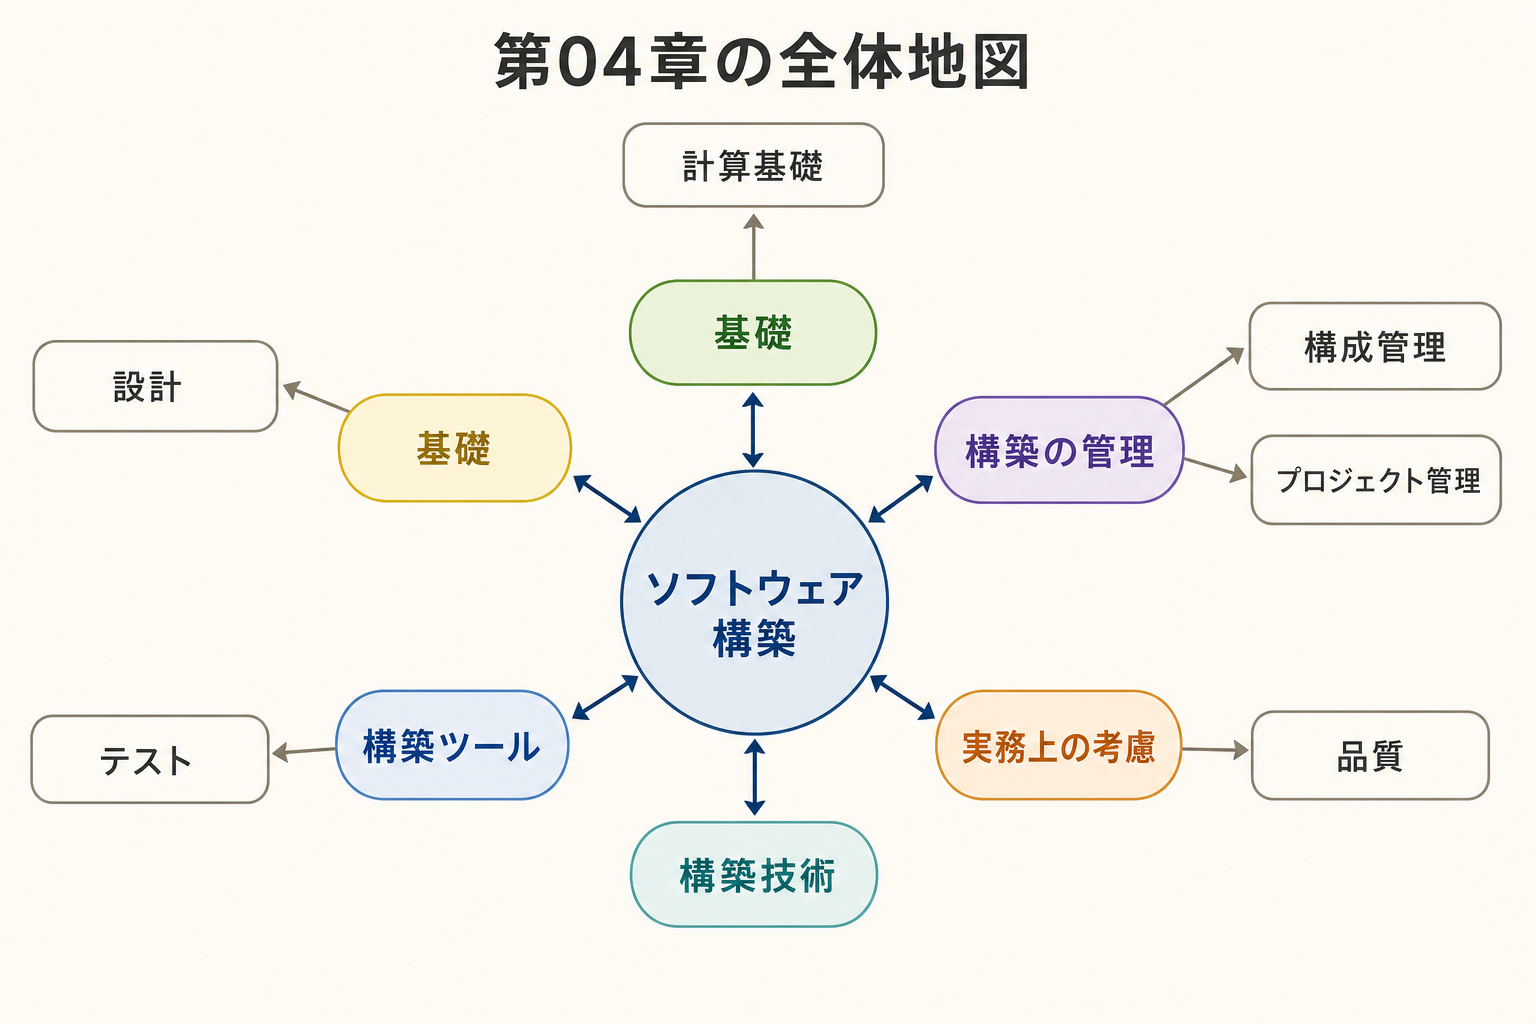
\includegraphics[width=0.96\linewidth]{assets/generated_figures/ch04/fig-ch04-01.png}}{\fbox{\parbox[c][48mm][c]{0.9\linewidth}{\centering 画像生成待ち\\第04章の全体地図}}}
\caption{第04章の全体地図}
\label{fig:ch04-01}
\end{figure}

\subsection*{最初に必要な用語}
\addcontentsline{toc}{subsection}{最初に必要な用語}

\par\smallskip\noindent\refstepcounter{table}\label{tab:ch04-01}\textbf{表 \thetable: 第04章 ソフトウェア構築 表01}\par\smallskip
\begin{longtable}{L{0.23\linewidth}L{0.69\linewidth}}
\toprule
\textbf{用語} & \textbf{初学者向けの説明} \\
\midrule
ソフトウェア構築 & ソフトウェアを詳細に作成・保守する活動である。コーディング、検証、単体テスト、統合テスト、デバッグなどを含む。 \\
コーディング & プログラミング言語などを使い、設計や要求を実行可能な形に書き表すこと。 \\
検証 & 作ったものが、仕様、設計、標準、期待された振る舞いを満たしているか確認すること。 \\
単体テスト & クラス、関数、モジュールなど、個別の部品を単独で確認するテスト。 \\
統合テスト & 複数の部品を組み合わせたとき、相互作用が正しく働くかを確認するテスト。 \\
デバッグ & 失敗の原因となる欠陥を見つけ、原因を理解し、修正する作業。 \\
依存関係 & 自分のソフトウェアが利用する外部ライブラリ、フレームワーク、部品、サービスなどとの関係。 \\
継続的統合 & 変更を頻繁に統合し、自動ビルドと自動テストで早く問題を発見する実践。 \\
再利用 & 既存の部品、コード、ライブラリ、サービス、設計パターンなどを別の問題解決に使うこと。 \\
API & アプリケーションプログラミングインタフェースのことである。ライブラリやサービスを利用するために公開された操作、引数、意味の取り決めである。 \\
\bottomrule
\end{longtable}

\subsection*{略語}
\addcontentsline{toc}{subsection}{略語}

\par\smallskip\noindent\refstepcounter{table}\label{tab:ch04-02}\textbf{表 \thetable: 第04章 ソフトウェア構築 表02}\par\smallskip
\begin{longtable}{L{0.16\linewidth}L{0.32\linewidth}L{0.44\linewidth}}
\toprule
\textbf{略語} & \textbf{日本語} & \textbf{説明} \\
\midrule
API & アプリケーションプログラミングインタフェース & ライブラリ、サービス、フレームワークを使うための公開された入り口。 \\
CI & 継続的統合 & 変更を頻繁に統合し、自動ビルドと自動テストで確認する実践。 \\
COTS & 商用既製品 & 自作ではなく、市販または既存の製品として利用するソフトウェア部品。 \\
DSL & ドメイン固有言語 & 特定領域の問題を表しやすいように作られた言語。 \\
IDE & 統合開発環境 & 編集、ビルド、テスト、デバッグなどを統合した開発環境。 \\
MDA & モデル駆動アーキテクチャ & モデルから実装へ変換する考え方を中心にした開発方式。 \\
PIM & プラットフォーム非依存モデル & 特定の実装環境に依存しない解決策のモデル。 \\
PSM & プラットフォーム固有モデル & 実装環境の詳細を含むモデル。 \\
TDD & テスト駆動開発 & テストを先に書き、そのテストを通すようにコードを書く開発スタイル。 \\
WYSIWYG & 見たままが得られる方式 & 画面上の見た目が成果物の見た目に近い編集方式。 \\
\bottomrule
\end{longtable}

\subsection*{導入：ソフトウェア構築とは何か}
\addcontentsline{toc}{subsection}{導入：ソフトウェア構築とは何か}

ソフトウェア構築とは、ソフトウェアを詳細に作成し、保守する活動である。具体的には、コーディング、検証、単体テスト、統合テスト、デバッグを含む。構築は、設計書の内容をただ機械的に写す作業ではない。多くの現場では、詳細な設計判断の一部が構築中に行われる。たとえば、どのデータ構造を使うか、エラーをどこで検出するか、処理をどの関数に分けるか、どのライブラリを使うかは、構築段階で決まることが多い。

この章の知識領域は、他の知識領域と強く結びつく。設計の成果物を入力として使い、テストに渡す成果物を作るため、ソフトウェア設計とソフトウェアテストとの関係が特に強い。また、構築ではソースファイル、テストケース、設定ファイル、文書など多数の構成品目が生まれるため、ソフトウェア構成管理とも密接に関係する。品質、プロジェクト管理、計算基礎とも関係が深い。

\begin{keybox}{重要}
ソフトウェア構築は、実装だけでなく「実装を検証可能にし、変更可能にし、統合可能にし、保守可能にする活動」である。したがって、構築の品質は、完成したソフトウェアの品質だけでなく、後続の変更や運用のしやすさにも影響する。
\end{keybox}

\begin{figure}[htbp]
\centering
\IfFileExists{assets/generated_figures/ch04/fig-ch04-02.png}{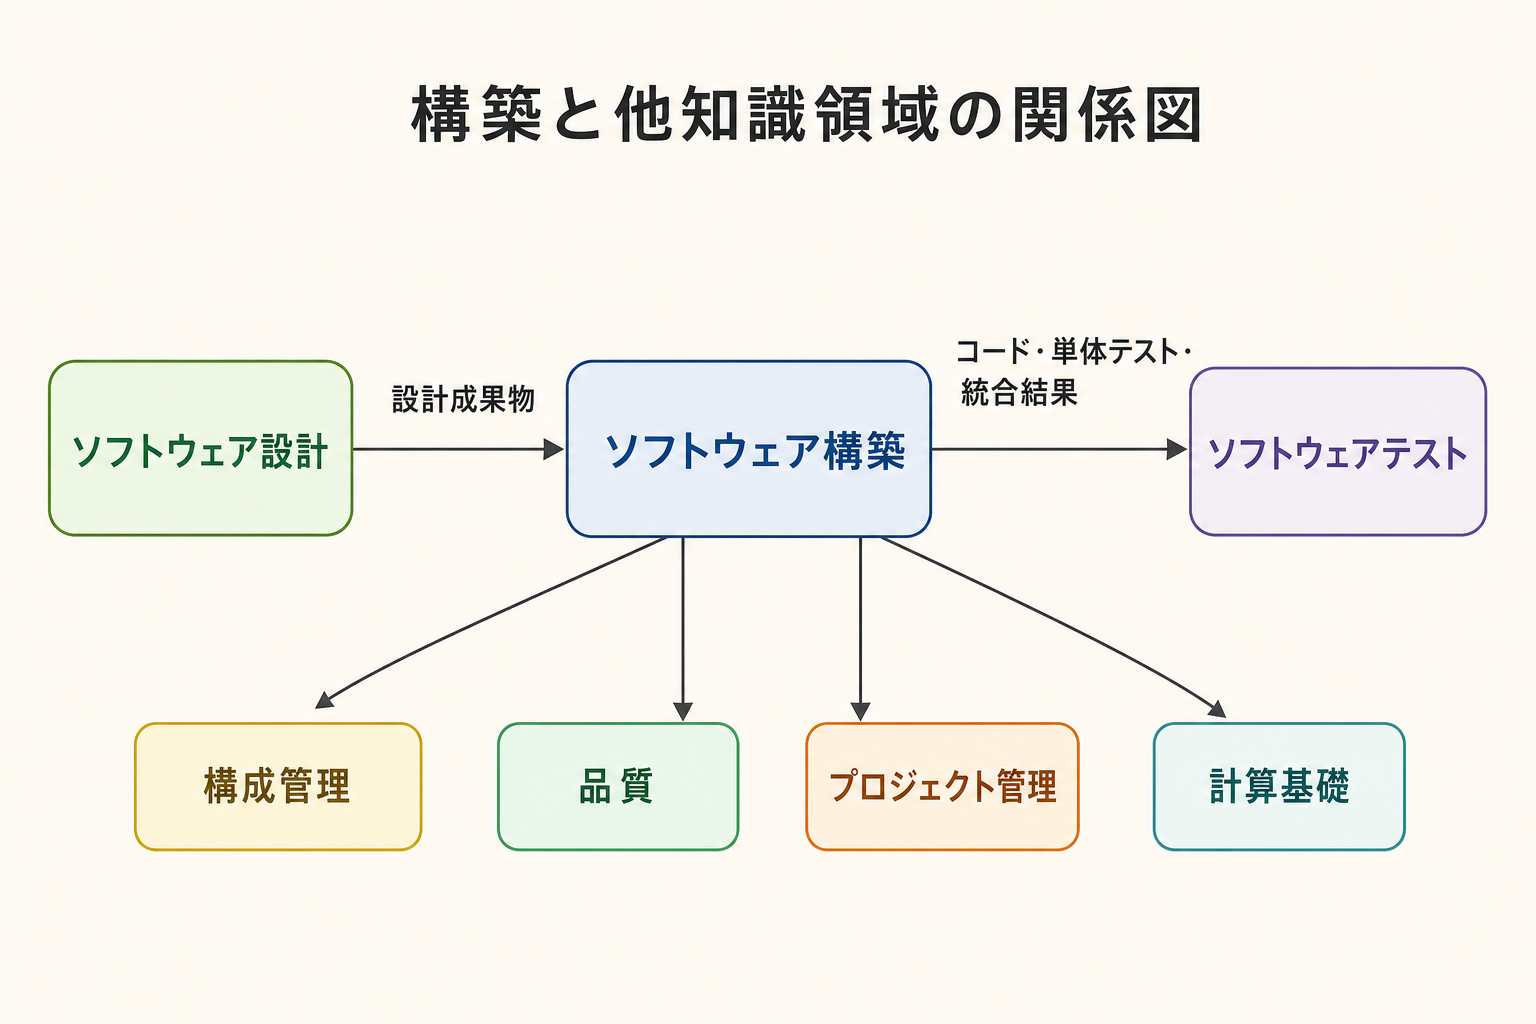
\includegraphics[width=0.96\linewidth]{assets/generated_figures/ch04/fig-ch04-02.png}}{\fbox{\parbox[c][48mm][c]{0.9\linewidth}{\centering 画像生成待ち\\構築と他知識領域の関係図}}}
\caption{構築と他知識領域の関係図}
\label{fig:ch04-02}
\end{figure}

\subsection{ソフトウェア構築の基礎}

ソフトウェア構築の基礎は、五つの考え方で整理できる。第一に複雑さを最小化すること、第二に変化を予期し受け入れること、第三に検証しやすく作ること、第四に資産を再利用すること、第五に標準を適用することである。これらは設計にも当てはまるが、構築では特にコード、テスト、部品、ツールに直接表れる。

\begin{figure}[htbp]
\centering
\IfFileExists{assets/generated_figures/ch04/fig-ch04-03.png}{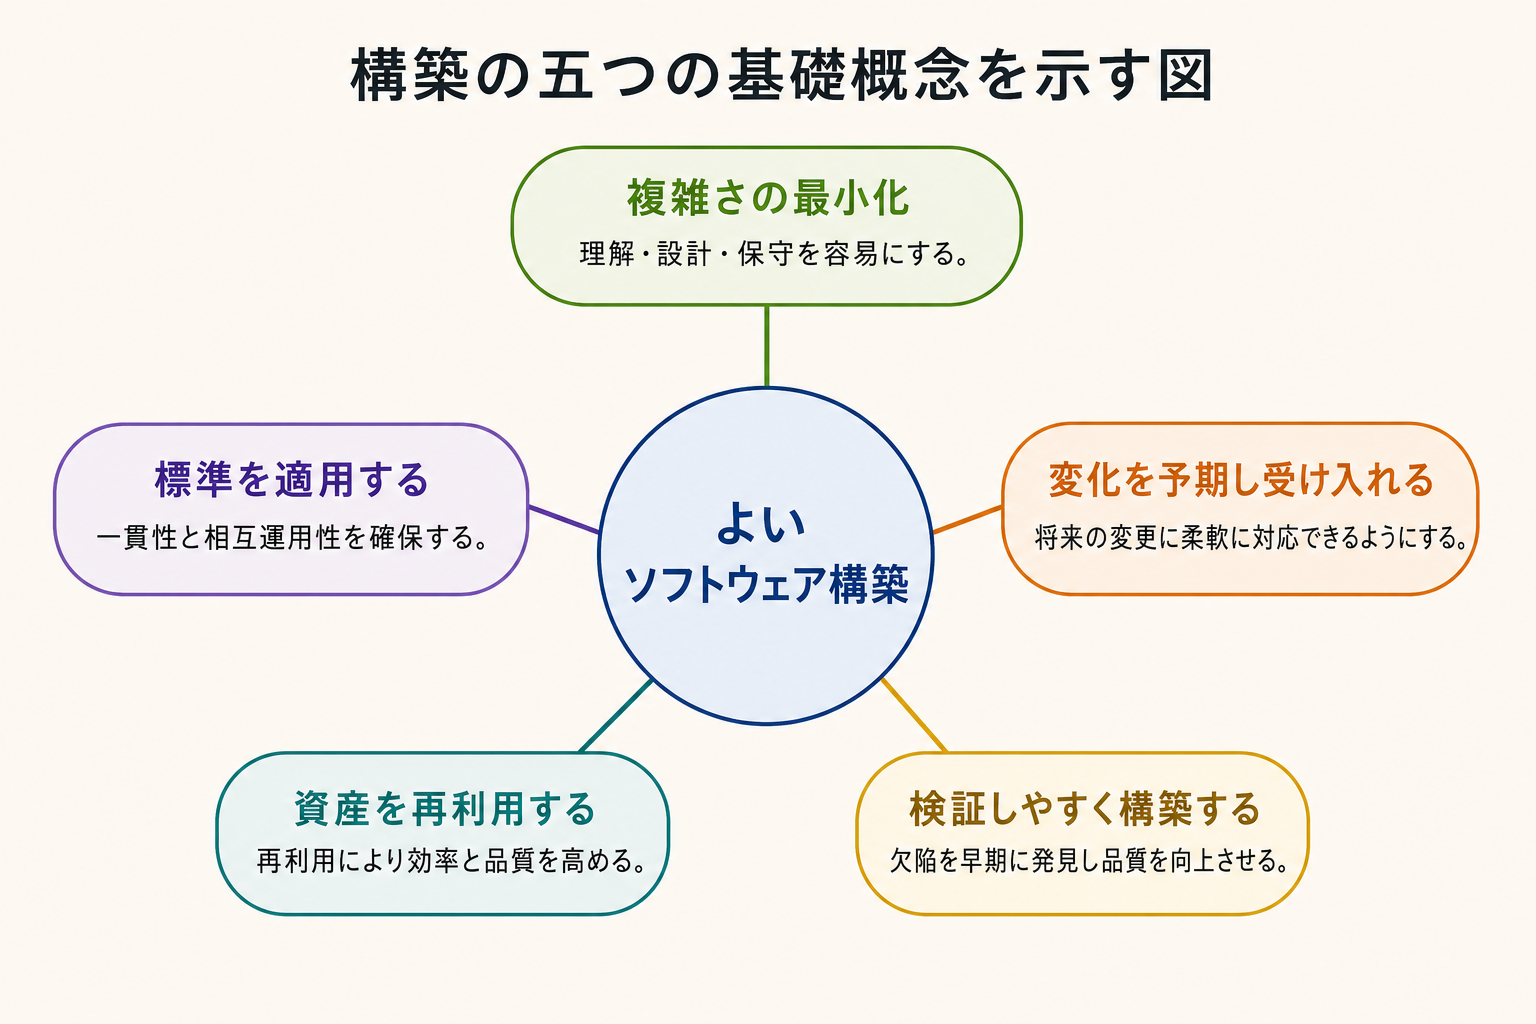
\includegraphics[width=0.96\linewidth]{assets/generated_figures/ch04/fig-ch04-03.png}}{\fbox{\parbox[c][48mm][c]{0.9\linewidth}{\centering 画像生成待ち\\構築の五つの基礎概念を示す図}}}
\caption{構築の五つの基礎概念を示す図}
\label{fig:ch04-03}
\end{figure}

\subsubsection{複雑さの最小化}

人間の作業記憶には限界がある。複雑な構造や大量の詳細を長時間正確に保持することは難しい。この限界は、ソフトウェア構築の中心課題である。コードが複雑になると、理解しにくく、テストしにくく、変更しにくくなる。したがって、構築では「賢そうなコード」よりも「単純で読みやすいコード」を優先する必要がある。

複雑さには複数の種類がある。条件分岐やループが多いコードは、実行経路が多くなる。依存関係が多いコードは、変更の影響範囲が広くなる。名前がわかりにくいコードは、読者の理解を妨げる。ビルド手順が複雑であれば、構築そのものが不安定になる。

循環的複雑度は、コードの制御フローの複雑さを測る代表的な指標である。大まかには、独立した実行経路の数を表す。値が大きいほど、理解やテストが難しくなる傾向がある。ただし、指標は判断の補助であり、指標だけでよいコードかどうかを決めてはならない。

複雑さを下げる実務上の手段には、命名規則、適切な関数分割、モジュール化、重複の排除、標準的な制御構造の利用、読みやすいレイアウト、レビュー、静的解析、単体テストがある。

\begin{keybox}{見分け方}
複雑なコードは、説明に時間がかかる。単純なコードは、名前、構造、流れから意図が読み取れる。構築では「動くか」だけでなく「次の人が読めるか」を基準にする必要がある。
\end{keybox}

\subsubsection{変化を予期し受け入れる}

多くのソフトウェアは時間とともに変わる。要求が変わることもあれば、利用者数、実行環境、ライブラリ、法規制、ビジネス方針が変わることもある。構築で変化を予期するとは、将来の変更が入ったときに、局所的な修正で済むように作ることである。

変化を予期するためには、拡張しやすい構造、明確なインタフェース、設定による切り替え、再利用可能な部品、テストによる安全網が必要である。一方で、まだ必要でない過剰な柔軟性を作り込むと、逆に複雑さが増える。したがって、予期すべき変化を見極め、過剰設計を避けることが重要である。

現代の開発では、変化を避けるのではなく受け入れる実践が広く使われる。アジャイル開発、DevOps、継続的デリバリ、継続的デプロイは、短い周期で変更を入れ、テストし、提供し、運用から学ぶための仕組みである。

\subsubsection{検証しやすく構築する}

検証しやすく構築するとは、コードを書いた人、テスト担当者、利用者が欠陥を見つけやすいようにソフトウェアを作ることである。これは、後でテストを追加すればよいという意味ではない。構築中から、テスト可能性を意識した設計と実装が必要である。

具体的には、単体テストを書きやすい関数分割、依存関係を差し替えやすい構造、複雑な言語機能の制限、ログによる挙動記録、コーディング標準、コードレビュー、入力値の検査、異常系の明示が役立つ。

検証しやすいコードでは、失敗が早く発見される。失敗が早く見つかるほど、原因に近い場所で修正できるため、修正費用を下げやすい。

\subsubsection{資産の再利用}

再利用とは、既存の資産を別の問題解決に使うことである。構築で再利用される資産には、フレームワーク、ライブラリ、モジュール、コンポーネント、ソースコード、商用既製品、クラウドサービスなどがある。

再利用には二つの側面がある。第一は、再利用されることを意識して作る「再利用のための構築」である。第二は、既存の資産を使って新しい解決策を作る「再利用による構築」である。前者では、汎用性、可変性、文書化、テストが重要になる。後者では、選定、評価、統合、ライセンス、保守、脆弱性管理が重要になる。

\begin{keybox}{注意}
再利用は必ず得とは限らない。再利用した部品に脆弱性、ライセンス問題、保守停止、過剰な依存があれば、後から大きな費用が発生する。再利用するものは、品質と責任範囲を確認する必要がある。
\end{keybox}

\subsubsection{構築における標準の適用}

標準は、構築を効率化し、品質を安定させ、複数人の作業をそろえるために使う。標準には外部標準と内部標準がある。外部標準は、業界団体、国際標準化機関、プラットフォーム提供者などが定める。内部標準は、組織やプロジェクトが定める。

構築に直接関係する標準には、文書形式、プログラミング言語、コーディング規約、例外処理方針、プラットフォームのインタフェース、ツール記法、UML などの表記法がある。特にセキュリティの観点では、許可する言語機能やライブラリ、禁止する危険な書き方を明確にすることが重要である。

\subsection{構築の管理}

構築は個人の作業に見えやすいが、実際には管理対象が多い。どのライフサイクルで進めるか、どの順で部品を作るか、いつ統合するか、何を測るか、どの依存関係を許すかによって、品質と進捗は大きく変わる。

\subsubsection{ライフサイクルモデルにおける構築}

ライフサイクルモデルによって、構築の位置づけは異なる。ウォーターフォール型や段階的提供型では、要求や設計がある程度完了した後に構築が始まる。この場合、構築は主にコーディングとデバッグとして見られやすい。

一方、進化的プロトタイピングやアジャイル開発では、要求、設計、構築、テストが重なり合う。短い反復の中で、必要な要求を具体化し、設計し、コードを書き、テストする。継続的デリバリや継続的デプロイでは、コード、テスト、提供、配置がさらに密接に結びつき、自動化されたパイプラインで実行される。

\begin{figure}[htbp]
\centering
\IfFileExists{assets/generated_figures/ch04/fig-ch04-04.png}{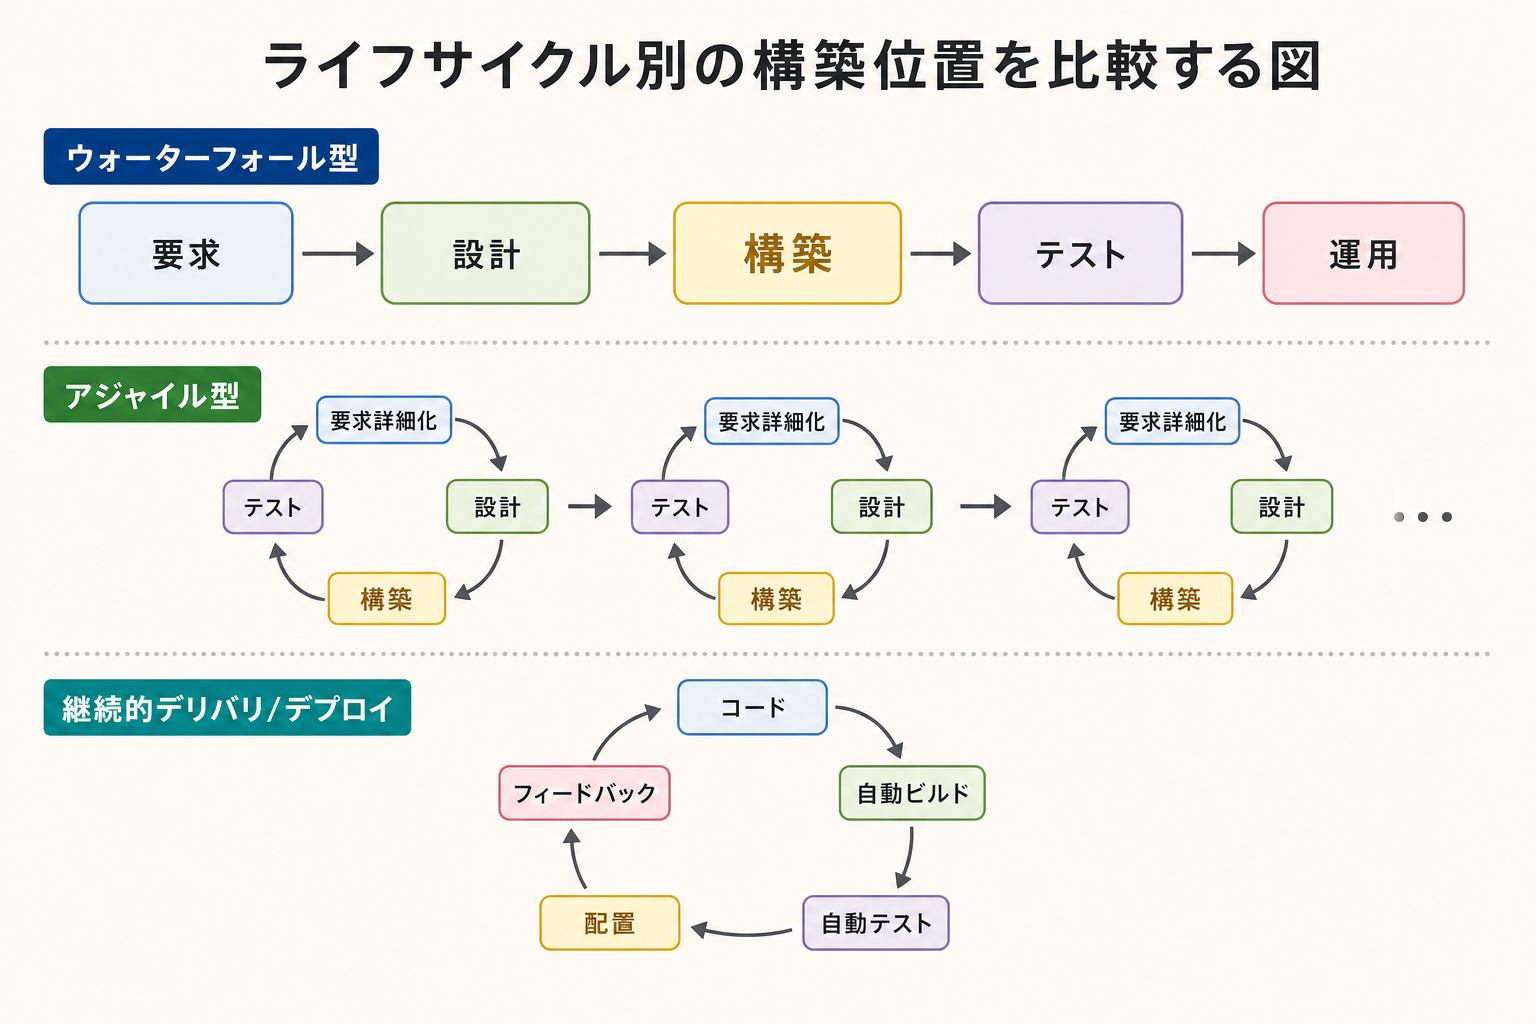
\includegraphics[width=0.96\linewidth]{assets/generated_figures/ch04/fig-ch04-04.png}}{\fbox{\parbox[c][48mm][c]{0.9\linewidth}{\centering 画像生成待ち\\ライフサイクル別の構築位置を比較する図}}}
\caption{ライフサイクル別の構築位置を比較する図}
\label{fig:ch04-04}
\end{figure}

\subsubsection{構築計画}

構築計画では、構築方法、部品の作成順序、統合順序、統合戦略、品質管理プロセス、担当割り当て、必要なツールや環境を決める。構築方法の選択は、複雑さの低減、変化への対応、検証しやすさに影響する。

たとえば、最初から全体を一度に統合する方針を選べば、初期の計画は単純に見えるが、問題発見が遅れる可能性がある。小さな部品を段階的に統合する方針を選べば、統合のための足場やテスト環境が必要になるが、問題を早く見つけやすい。

\subsubsection{構築測定}

構築では、多くの活動や成果物を測定できる。開発したコード量、変更したコード量、再利用したコード量、削除したコード量、コード複雑度、コードレビューで見つかった欠陥数、欠陥発見率、欠陥修正率、作業工数、予定との差分などである。

測定の目的は、管理と改善である。数値を集めるだけでは意味がない。たとえば、複雑度が高い箇所を重点的にレビューする、欠陥修正率から計画を見直す、再利用量から開発効率を評価する、といった使い方が必要である。

\subsubsection{依存関係の管理}

現代のソフトウェアは、多くの外部ライブラリやフレームワークに依存する。Java の Maven、JavaScript の NPM などのパッケージ管理ツールは、依存関係の導入、更新、削除を自動化する。しかし、依存関係は便利である一方、リスクも運ぶ。

依存関係の集合は、供給網のようなネットワークを作る。直接使っているライブラリが、さらに別のライブラリに依存していることも多い。どこかに脆弱性、ライセンス衝突、保守停止、悪意あるコードがあれば、自分の製品にも影響する。

依存関係管理では、不要な依存を避ける、信頼できる依存だけを使う、ライセンスを確認する、脆弱性情報を監視する、バージョン更新を計画する、ロックファイルやソフトウェア部品表を活用する、といった実践が重要である。

\begin{figure}[htbp]
\centering
\IfFileExists{assets/generated_figures/ch04/fig-ch04-05.png}{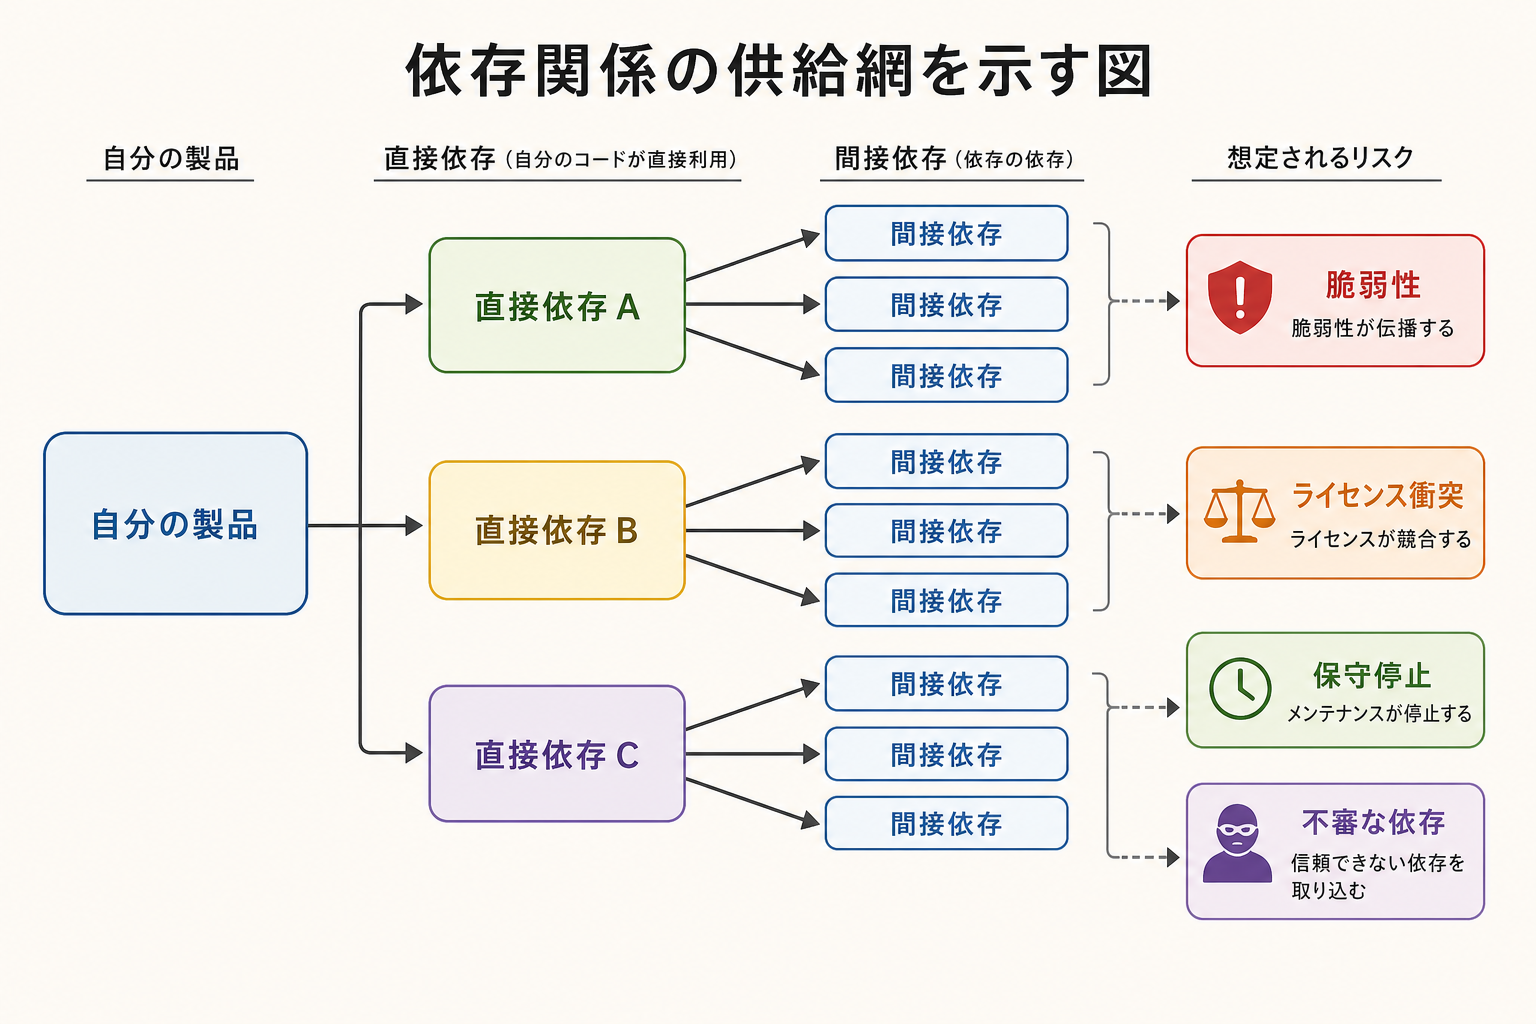
\includegraphics[width=0.96\linewidth]{assets/generated_figures/ch04/fig-ch04-05.png}}{\fbox{\parbox[c][48mm][c]{0.9\linewidth}{\centering 画像生成待ち\\依存関係の供給網を示す図}}}
\caption{依存関係の供給網を示す図}
\label{fig:ch04-05}
\end{figure}

\subsection{実務上の考慮}

構築は、現実の制約の中で進む。要求は変わり、設計は不完全で、利用できる人員や時間には限りがあり、外部サービスやライブラリにも制約がある。そのため、構築は理論だけでなく、実務的な判断が重要な活動である。

\subsubsection{構築設計}

構築段階でも設計は行われる。要求分析や上位設計で決まっていない詳細を、構築中に決める必要があるためである。たとえば、アルゴリズム、データ構造、関数やクラスの責務、インタフェース、例外の扱い、ログの粒度などは、構築中に具体化されることが多い。

建築現場で、図面に書かれていない細部を現場で調整する必要があるのと同じで、ソフトウェア構築でも詳細の調整が必要である。ただし、場当たり的に決めるのではなく、設計原則、標準、テスト容易性、変更容易性に基づいて判断する必要がある。

\subsubsection{構築言語}

構築言語とは、人間がコンピュータに実行可能な解決策を指定するための言語である。狭い意味のプログラミング言語だけでなく、設定言語、ツールキット言語、スクリプト言語、ドメイン固有言語も含む。

\par\smallskip\noindent\refstepcounter{table}\label{tab:ch04-03}\textbf{表 \thetable: 第04章 ソフトウェア構築 表03}\par\smallskip
\begin{longtable}{L{0.24\linewidth}L{0.66\linewidth}}
\toprule
\textbf{構築言語の種類} & \textbf{説明} \\
\midrule
設定言語 & 限られた選択肢から設定を選び、ソフトウェアの振る舞いや導入形態を変える言語である。設定ファイルなどが該当する。 \\
ツールキット言語 & 特定の部品群やツールキットを組み合わせてアプリケーションを作るための言語である。 \\
スクリプト言語 & 自動化、処理の連結、簡易アプリケーションの構築によく使われる言語である。 \\
プログラミング言語 & 汎用的で柔軟な構築言語である。C/C++、Java、Python、C\# などが例である。 \\
ドメイン固有言語 & 特定の業務領域や技術領域の概念を直接表す言語である。汎用言語よりも領域内の問題を簡潔に表せることがある。 \\
\bottomrule
\end{longtable}

構築言語の表記法には、テキストを中心にする言語的表記、数学的に厳密な形式的表記、図形やアイコンを中心にする視覚的表記がある。言語選択は、性能、信頼性、移植性、セキュリティ、開発者の学習コストに影響する。

\begin{figure}[htbp]
\centering
\IfFileExists{assets/generated_figures/ch04/fig-ch04-06.png}{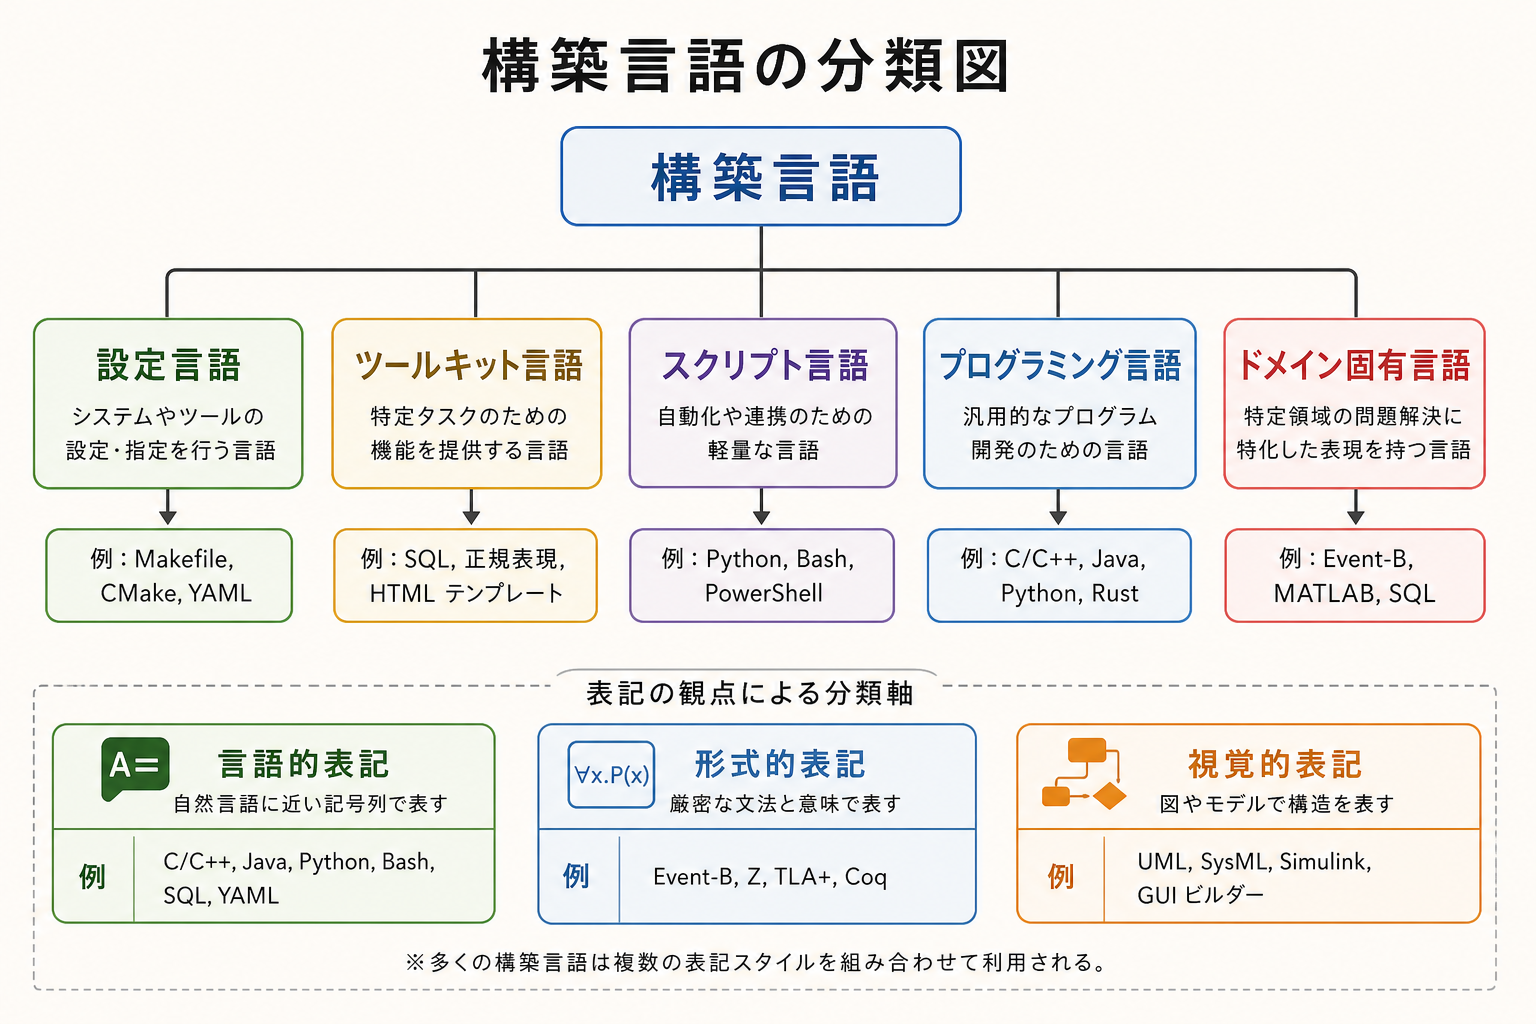
\includegraphics[width=0.96\linewidth]{assets/generated_figures/ch04/fig-ch04-06.png}}{\fbox{\parbox[c][48mm][c]{0.9\linewidth}{\centering 画像生成待ち\\構築言語の分類図}}}
\caption{構築言語の分類図}
\label{fig:ch04-06}
\end{figure}

\subsubsection{コーディング}

コーディングでは、ソースコードを理解しやすく、変更しやすく、検証しやすく書くことが重要である。単に動作するコードを書くだけでは不十分である。コードは、将来の読者に意図を伝える文書でもある。

構築におけるコーディングの主な考慮事項は次のとおりである。

\begin{itemize}
  \item 命名規則、字下げ、レイアウトにより、理解しやすいソースコードを作る。
  \item クラス、列挙型、変数、名前付き定数などを適切に使う。
  \item 条件分岐、ループ、例外処理などの制御構造を過度に複雑にしない。
  \item 予期できるエラーと例外的なエラーを区別して扱う。
  \item バッファオーバーフロー、配列範囲外参照、入力検証不足など、コードレベルのセキュリティ問題を防ぐ。
  \item スレッド、データベースロック、ファイル、ネットワーク接続などの資源を適切に扱う。
  \item コードを関数、クラス、パッケージなどに整理する。
  \item 必要な文書化とコメントを行う。
  \item 測定に基づいて性能を調整する。
\end{itemize}

\begin{keybox}{コメントの考え方}
コメントは、コードの日本語訳ではない。よいコメントは、コードだけでは読み取りにくい理由、前提、制約、例外、意図を説明する。名前と構造で伝えられることは、名前と構造で伝える方がよい。
\end{keybox}

\subsubsection{構築テスト}

構築では、主に単体テストと統合テストが行われる。これらは、多くの場合、コードを書いたソフトウェア技術者自身が実行する。構築テストの目的は、欠陥が混入してから発見されるまでの時間差を短くし、修正費用を下げることである。

単体テストは、関数、クラス、モジュールなどを単独で確認する。統合テストは、それらを組み合わせたときに正しく相互作用するかを確認する。構築テストは、通常、システムテスト、アルファテスト、ベータテスト、ストレステスト、使用性テストなどの広い範囲のテストまでは含まない。

テストケースは、コードを書いた後に作られることもあるが、コードを書く前に作られることもある。テストを先に書く方法は、テストファーストプログラミングまたはテスト駆動開発として扱われる。

\subsubsection{構築における再利用}

構築における再利用には、再利用のための構築と、再利用による構築がある。再利用のための構築では、将来別の場所で使えるように、部品を作る。可変性を設定で変えられるようにする、使い方を文書化する、単体テストを整備する、公開方法を整えるといった作業が必要である。

再利用による構築では、既存の部品を使って新しいソフトウェアを作る。ライブラリ、フレームワーク、オープンソース部品、商用既製品、クラウドサービスが代表例である。クラウドサービスを利用する場合、認証、メッセージング、ストレージなどを外部のサービスへ委任できる。このような形は、バックエンドサービスとしての利用とも呼ばれる。

再利用では、部品を選び、評価し、統合し、テストし、利用情報を記録する必要がある。ライセンス、保守状況、脆弱性、利用条件を確認しない再利用は、後のリスクになる。

\subsubsection{構築品質}

構築品質は、コードやその近くにある成果物の品質に焦点を当てる。要求や上位設計に関する品質活動も重要だが、構築品質では、詳細設計、コード、単体テスト、統合テスト、ビルド、静的解析、レビューが中心になる。

構築品質を高める主な技法には、単体テスト、統合テスト、テストファースト開発、表明、防御的プログラミング、デバッグ、コードインスペクション、技術レビュー、セキュリティレビュー、静的解析がある。

特にセキュリティでは、よく知られた脆弱性パターンを避ける必要がある。入力検証不足、境界チェック不足、例外の握りつぶし、危険なライブラリの利用、認可確認漏れなどは、構築段階で入りやすい問題である。

\subsubsection{統合}

統合とは、個別に作られた関数、クラス、部品、サブシステムを一つのシステムへ組み合わせることである。さらに、他のソフトウェアやハードウェアと接続することも統合に含まれる。

統合には、段階的統合と一括統合がある。一括統合は、すべての部品ができてからまとめて結合する方法であり、ビッグバン統合とも呼ばれる。問題発見が遅れやすい。段階的統合は、小さな単位から順に組み合わせる方法であり、エラーの場所を特定しやすく、進捗を把握しやすい。

段階的統合では、まだ存在しない部品の代役として、スタブ、ドライバ、モックオブジェクトなどの足場が必要になることがある。現代では、継続的統合によって、変更のたびに自動的にビルドとテストを行うことが広く使われる。

\begin{figure}[htbp]
\centering
\IfFileExists{assets/generated_figures/ch04/fig-ch04-07.png}{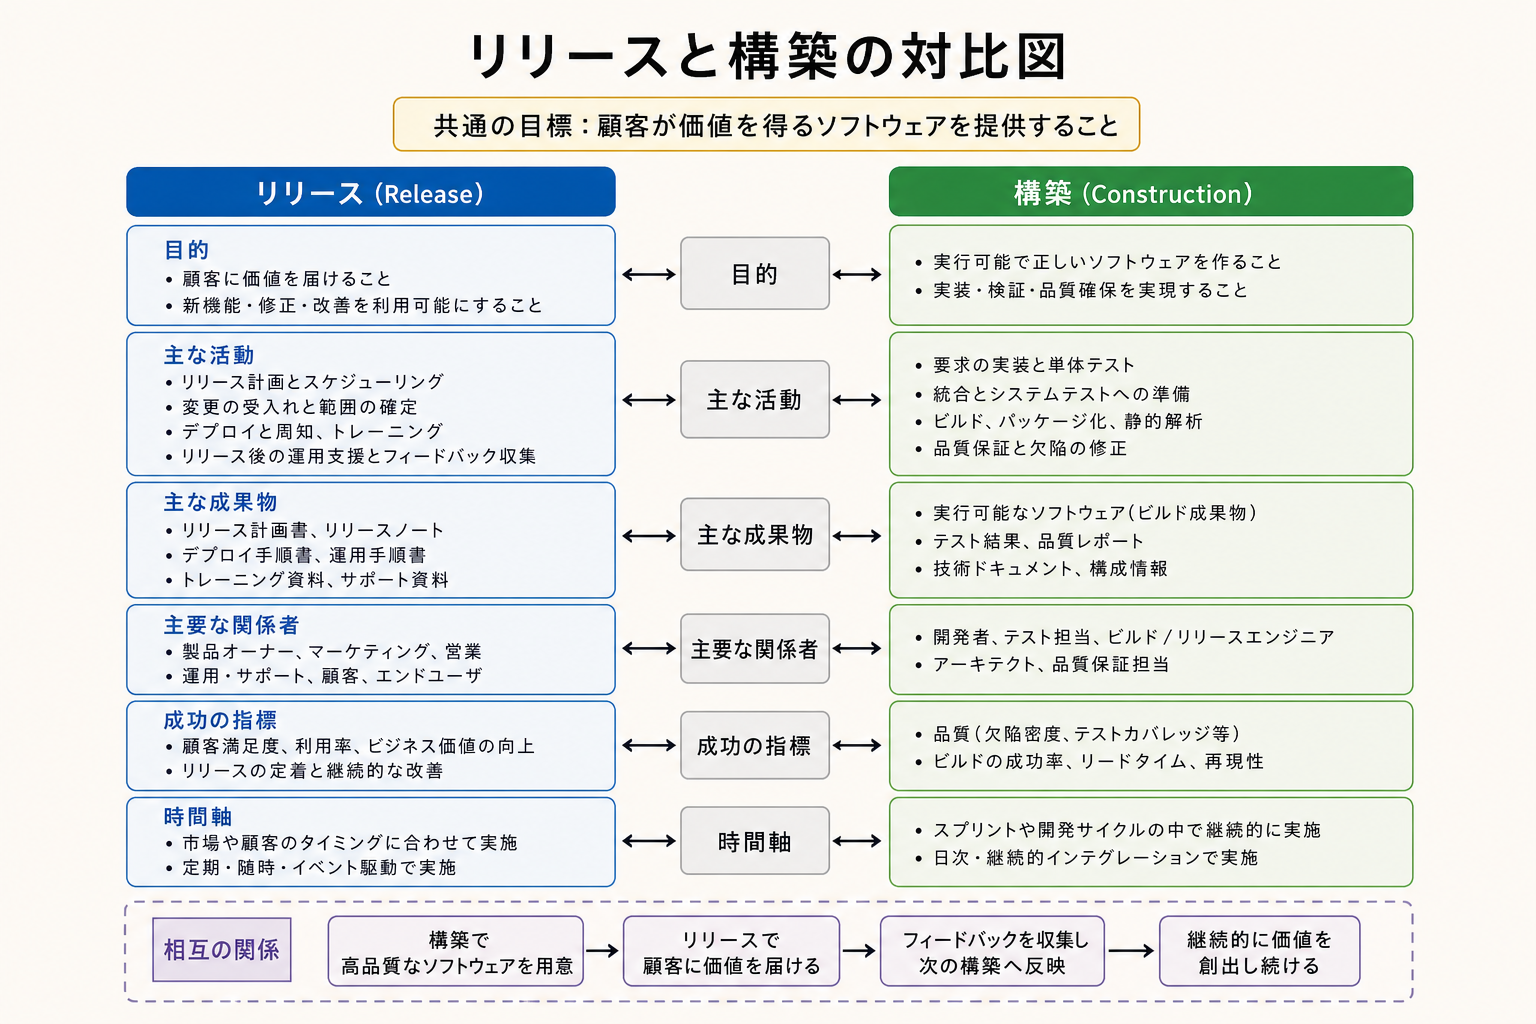
\includegraphics[width=0.96\linewidth]{assets/generated_figures/ch04/fig-ch04-07.png}}{\fbox{\parbox[c][48mm][c]{0.9\linewidth}{\centering 画像生成待ち\\段階的統合と継続的統合の流れ}}}
\caption{段階的統合と継続的統合の流れ}
\label{fig:ch04-07}
\end{figure}

\subsubsection{クロスプラットフォーム開発と移行}

モバイルアプリケーションなどは、特定のプラットフォームに強く依存することが多い。たとえば、iOS と Android では、開発環境、API、利用できる機能、利用者体験が異なる。各プラットフォーム向けに別々に開発すると、費用と時間が増え、実装差も生まれやすい。

クロスプラットフォーム開発は、共通の言語やフレームワークで作り、複数のプラットフォームに出力する方法である。方式としては、共通言語から各プラットフォーム向けのネイティブアプリを生成する方法と、Web 技術で作った部分をネイティブのコンテナで包むハイブリッド方式がある。

既存アプリケーションを別のプラットフォームへ移す場合は、移行が必要になる。移行では、プログラミング言語の違い、API の違い、データ形式、テスト環境、利用者体験の差を考慮する必要がある。

\subsection{構築技術}

構築技術は、実際にコードや実行可能なソフトウェアを作るための具体的な方法である。この章では、API、オブジェクト指向、総称、表明、例外処理、実行可能モデル、状態機械、設定、国際化、構文解析、並行処理、ミドルウェア、分散・クラウド、異種システム、性能、標準、テストファースト、フィードバックループを扱う。

\subsubsection{API の設計と利用}

API は、ライブラリやフレームワーク、サービスを利用するために公開された操作の集合である。API は、関数名や引数の型といった署名だけでなく、その操作が何を意味し、どのような効果を持つかという意味も含む。

よい API は、学びやすく、覚えやすく、読みやすいコードにつながり、誤用しにくく、拡張しやすく、必要な機能を十分に備え、後方互換性を保ちやすい。広く使われるライブラリやサービスでは、実装よりも API の方が長く生きることが多いため、API は安定性が重要である。

Web API では、RESTful API や OpenAPI のような標準的な記述がよく使われる。API ファーストとは、アプリケーションの内部実装より先に API の契約を設計し、その契約に基づいてサーバ側とクライアント側を作る考え方である。

\begin{figure}[htbp]
\centering
\IfFileExists{assets/generated_figures/ch04/fig-ch04-08.png}{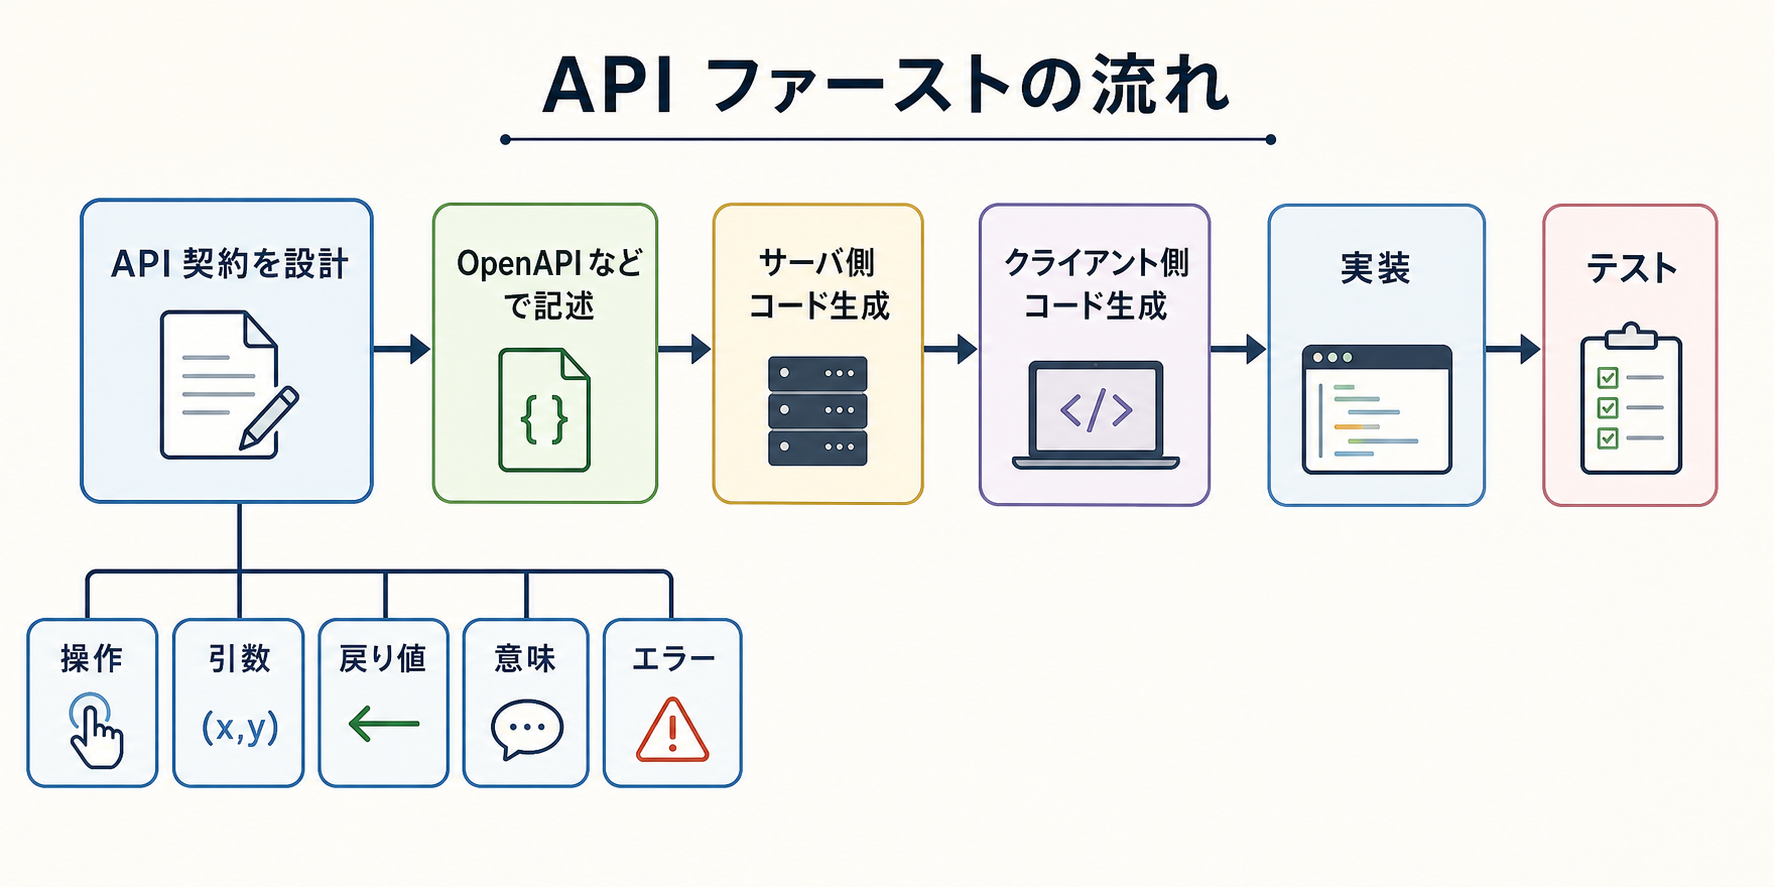
\includegraphics[width=0.96\linewidth]{assets/generated_figures/ch04/fig-ch04-08.png}}{\fbox{\parbox[c][48mm][c]{0.9\linewidth}{\centering 画像生成待ち\\API ファーストの流れ}}}
\caption{API ファーストの流れ}
\label{fig:ch04-08}
\end{figure}

\subsubsection{オブジェクト指向の実行時問題}

オブジェクト指向言語には、実行時に振る舞いを決める仕組みがある。代表例は多態性と反射である。

多態性とは、一般的な操作を、実際の具体的なオブジェクトの種類に応じて実行時に決められる性質である。たとえば、同じ「描画する」という操作でも、円、四角形、文字列で実行される処理が異なる。このように実行時に呼び出し先が決まることを動的束縛という。

反射とは、プログラムが実行時に自分自身の構造や振る舞いを調べたり、変更したりできる性質である。たとえば、クラス名やメソッド名を文字列として扱い、実行時にオブジェクトを生成したり、メソッドを呼び出したりできる。

これらは柔軟性を高めるが、理解やテストを難しくすることがある。利用する場合は、意図を明確にし、過度に動的な構造を避ける必要がある。

\subsubsection{パラメータ化、テンプレート、総称}

パラメータ化された型は、型やクラスを定義するときに、利用する型の一部を後から与えられるようにする仕組みである。Java では総称、C++ ではテンプレートと呼ばれる。

たとえば、整数のリスト、文字列のリスト、顧客オブジェクトのリストを別々に作るのではなく、「任意の型 T のリスト」として定義し、利用時に T を指定できる。これにより、型安全性を保ちながら再利用しやすい部品を作れる。

\subsubsection{表明、契約による設計、防御的プログラミング}

表明とは、プログラム中に置かれる実行可能な条件式である。プログラムが想定する前提や不変条件が成り立っているかを実行時に確認する。開発時には欠陥を早く見つける助けになる。

契約による設計とは、各関数やクラスについて、呼び出し前に満たすべき事前条件、呼び出し後に保証する事後条件、常に守られる不変条件を明確にする考え方である。これにより、部品同士の責任範囲が明確になる。

防御的プログラミングとは、不正な入力や想定外の状態から関数を守るために、入力値を検査し、異常な場合の処理を決めることである。防御的に書くことで、欠陥の影響を局所化しやすい。

\begin{figure}[htbp]
\centering
\IfFileExists{assets/generated_figures/ch04/fig-ch04-09.png}{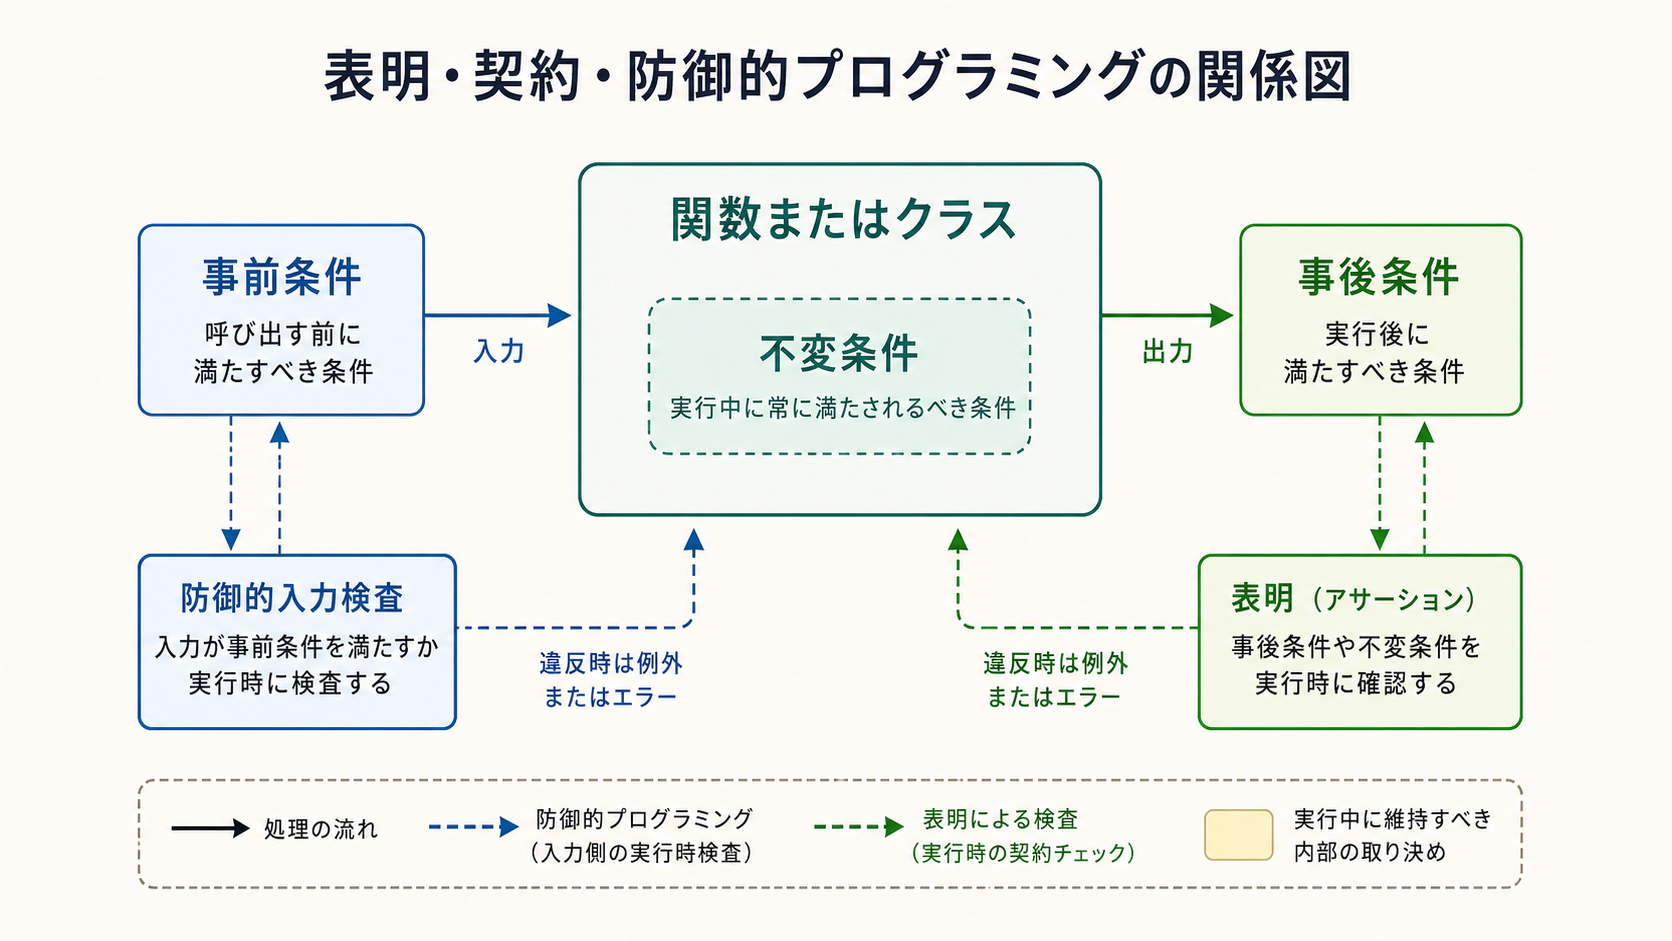
\includegraphics[width=0.96\linewidth]{assets/generated_figures/ch04/fig-ch04-09.png}}{\fbox{\parbox[c][48mm][c]{0.9\linewidth}{\centering 画像生成待ち\\表明・契約・防御的プログラミングの関係図}}}
\caption{表明・契約・防御的プログラミングの関係図}
\label{fig:ch04-09}
\end{figure}

\subsubsection{エラー処理、例外処理、フォールトトレランス}

エラー処理の方法は、正しさ、頑健性、信頼性に影響する。エラー処理には、警告ログを出す、エラーコードを返す、中立値を返す、次の有効データを使う、処理を停止するなど、複数の方法がある。どれを使うかは、利用者への影響、データの重要性、安全性、復旧可能性によって変わる。

例外処理は、エラーや例外的な出来事を検出し、処理する仕組みである。基本的には、例外を送出し、対応する処理ブロックで捕捉する。例外メッセージには、原因理解に必要な情報を含めるべきである。空の捕捉ブロックで例外を握りつぶすと、問題の発見が遅れる。

フォールトトレランスとは、エラーを検出し、回復するか、影響を閉じ込めることで、ソフトウェアの信頼性を高める技法群である。再試行、補助コード、投票アルゴリズム、値の代替などがある。

\subsubsection{実行可能モデル}

実行可能モデルとは、特定のプログラミング言語や実装構造の詳細から離れて、実行できる形で振る舞いを表すモデルである。実行可能 UML などが例である。

モデル駆動アーキテクチャでは、プラットフォーム非依存モデルとプラットフォーム固有モデルを区別する。プラットフォーム非依存モデルは、実装環境に依存しない解決策を表す。プラットフォーム固有モデルは、特定のハードウェアやソフトウェア環境の詳細を含む。変換器は、非依存モデルとプラットフォーム情報を組み合わせ、実装を生成する。

\begin{figure}[htbp]
\centering
\IfFileExists{assets/generated_figures/ch04/fig-ch04-10.png}{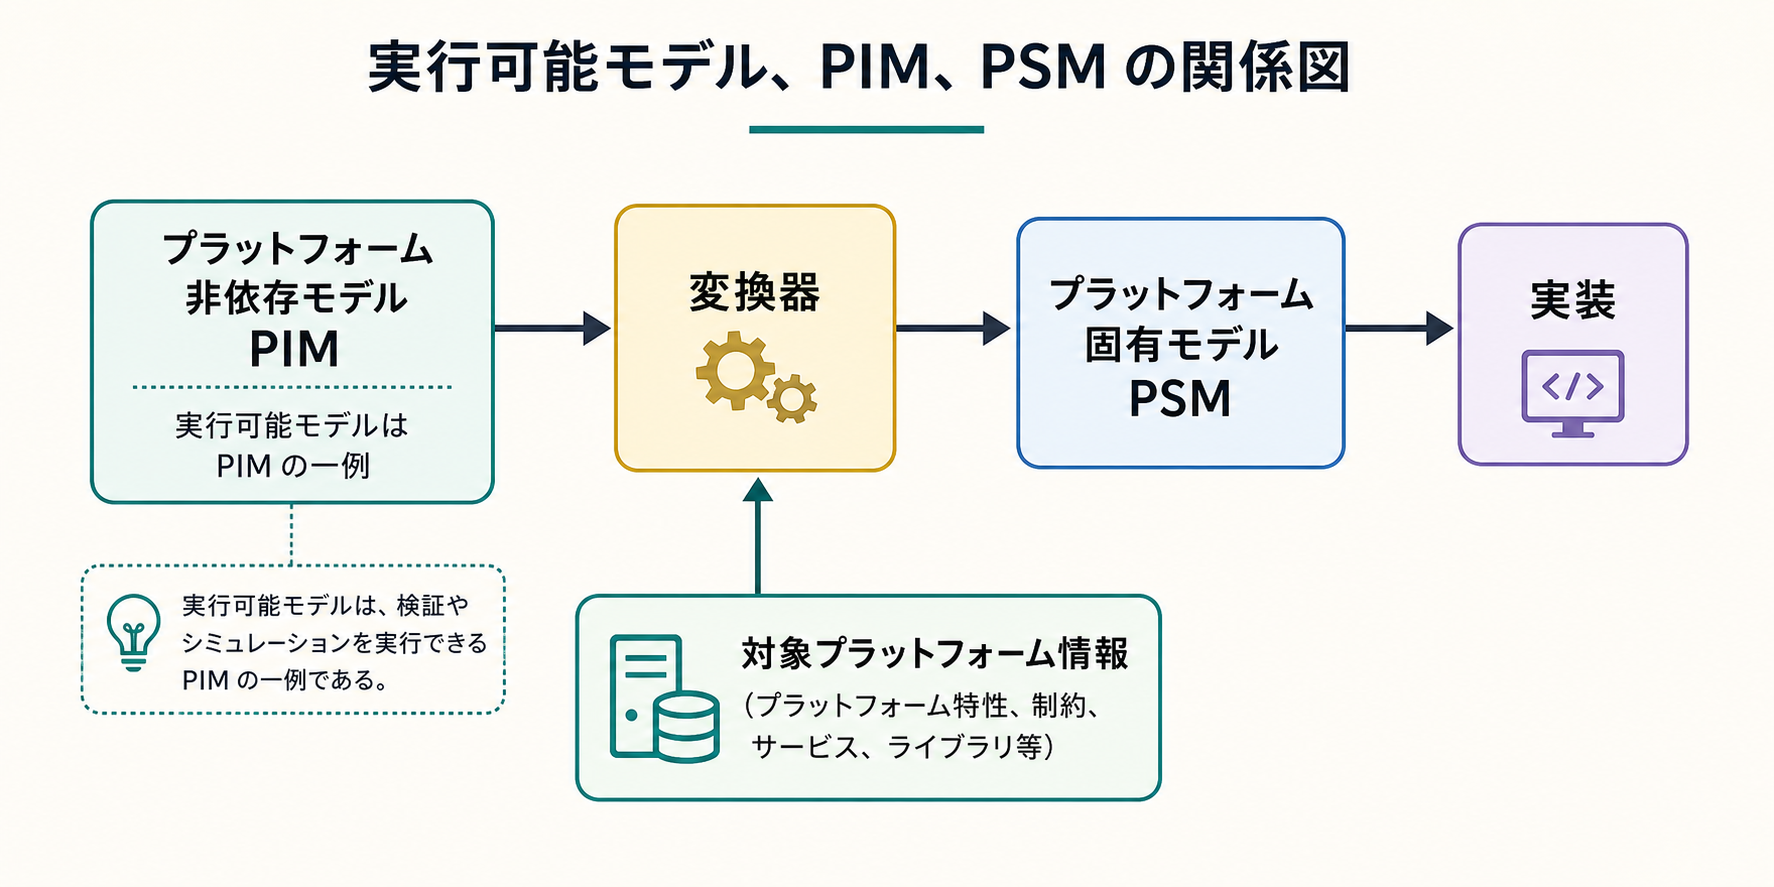
\includegraphics[width=0.96\linewidth]{assets/generated_figures/ch04/fig-ch04-10.png}}{\fbox{\parbox[c][48mm][c]{0.9\linewidth}{\centering 画像生成待ち\\実行可能モデル、PIM、PSM の関係図}}}
\caption{実行可能モデル、PIM、PSM の関係図}
\label{fig:ch04-10}
\end{figure}

\subsubsection{状態に基づく構築技法と表駆動構築技法}

状態に基づくプログラミングは、有限状態機械を使ってプログラムの振る舞いを表す技法である。状態、イベント、遷移、動作を明確にすることで、複雑な分岐を整理できる。状態遷移図は、仕様、実装、デバッグ、文書化で使える。

表駆動方式は、複雑な \texttt{if} 文や \texttt{case} 文の代わりに、表を使って情報を表す方法である。条件と処理の対応を表にまとめると、ロジックが見通しやすく、変更もしやすくなることがある。表駆動では、何を表に入れるか、どのように効率よく表を参照するかが重要である。

\begin{figure}[htbp]
\centering
\IfFileExists{assets/generated_figures/ch04/fig-ch04-11.png}{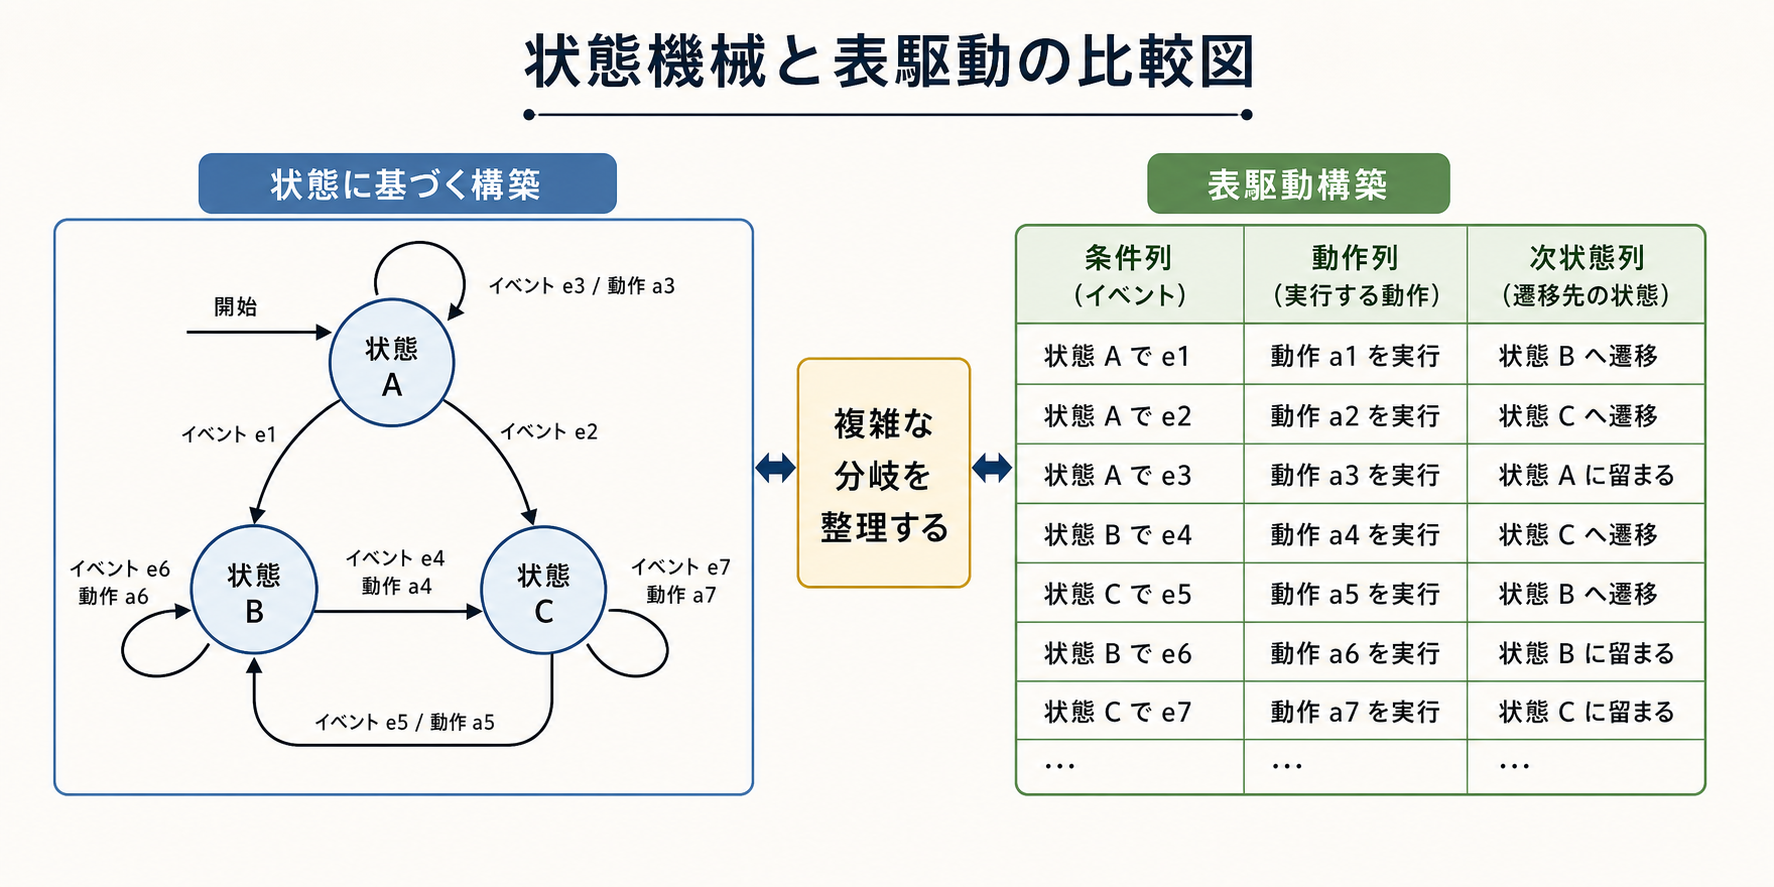
\includegraphics[width=0.96\linewidth]{assets/generated_figures/ch04/fig-ch04-11.png}}{\fbox{\parbox[c][48mm][c]{0.9\linewidth}{\centering 画像生成待ち\\状態機械と表駆動の比較図}}}
\caption{状態機械と表駆動の比較図}
\label{fig:ch04-11}
\end{figure}

\subsubsection{実行時設定と国際化}

実行時設定とは、プログラムの値や動作を、実行時に設定ファイルや環境変数などから読み取って決めることである。これにより、コードを変更せずに動作を変えられる。設定を使うことで柔軟性は高まるが、設定値の検証、既定値、変更履歴、機密情報の扱いが重要になる。

国際化とは、複数の言語や地域に対応できるようにソフトウェアを準備することである。これに対応して、特定の地域や言語に合わせる作業を地域化という。画面の文言、エラーメッセージ、日付形式、通貨、文字コード、並び順、右から左へ書く言語などを考慮する必要がある。

国際化を後から追加すると、コードのあちこちに埋め込まれた文字列や地域依存の処理を修正する必要がある。構築時から、文字列を外部化し、文字コードとロケールを意識することが重要である。

\subsubsection{文法に基づく入力処理}

文法に基づく入力処理は、入力を字句や構文の規則に従って解析する技法である。代表的な例は、プログラミング言語、設定ファイル、数式、検索式、通信プロトコルの解析である。

構文解析では、入力のトークン列から解析木または構文木と呼ばれるデータ構造を作る。解析木は、その入力がどのような構造を持つかを表す。構文解析の後、意味検査やシンボル表の確認を行い、計算処理や変換処理につなげる。

文法に基づく入力処理は、入力検証にも重要である。曖昧な文字列処理で入力を解釈すると、誤解析やセキュリティ問題につながる可能性がある。

\subsubsection{並行処理の基本部品}

並行処理では、複数の処理が同時または並行して進む。共有資源に同時にアクセスすると競合が起こるため、同期の仕組みが必要である。代表的な基本部品には、セマフォ、モニタ、ミューテックスがある。

セマフォは、複数のプロセスやスレッドが共有資源へアクセスする数を制御するための抽象である。モニタは、共有変数とその操作をひとまとまりにし、同時に一つの処理だけが内部で動くようにする抽象データ型である。ミューテックスは、共有資源への排他的アクセスを実現するための仕組みである。

並行処理の欠陥は再現しにくいことが多い。デッドロック、競合状態、ライブロック、可視性の問題などを避けるには、設計段階から同期方針を明確にし、テストとレビューを組み合わせる必要がある。

\subsubsection{ミドルウェア}

ミドルウェアとは、オペレーティングシステムより上、アプリケーションより下で、アプリケーションに共通サービスを提供するソフトウェアである。通信、メッセージング、永続化、トランザクション、名前解決、位置透過性などを提供することがある。

ミドルウェアは、部品同士を接続する役割を持つ。メッセージ指向ミドルウェアは、複数のアプリケーション間のメッセージ交換を支援する。企業サービスバスは、サービス指向の通信や連携を支える基盤として使われる。

\subsubsection{分散およびクラウド基盤ソフトウェアの構築方法}

分散システムは、物理的に離れた複数の計算機がネットワークで接続され、利用者に一体の資源や機能を提供するシステムである。分散ソフトウェアの構築では、並列性、通信、遅延、部分故障、整合性、セキュリティが問題になる。

分散プログラミングには、クライアントサーバ、三層アーキテクチャ、多層アーキテクチャ、分散オブジェクト、疎結合、密結合などの形がある。

クラウド基盤ソフトウェアでは、マイクロサービス、コンテナ、API ゲートウェイ、サービス登録と発見、監視、自動スケーリングなどを考慮する。従来の分散トランザクションでは ACID 特性を重視することが多い。一方、マイクロサービスでは、すべてを強い整合性で統一するのが難しく、SAGA などによる結果整合性を使うことがある。

\begin{figure}[htbp]
\centering
\IfFileExists{assets/generated_figures/ch04/fig-ch04-12.png}{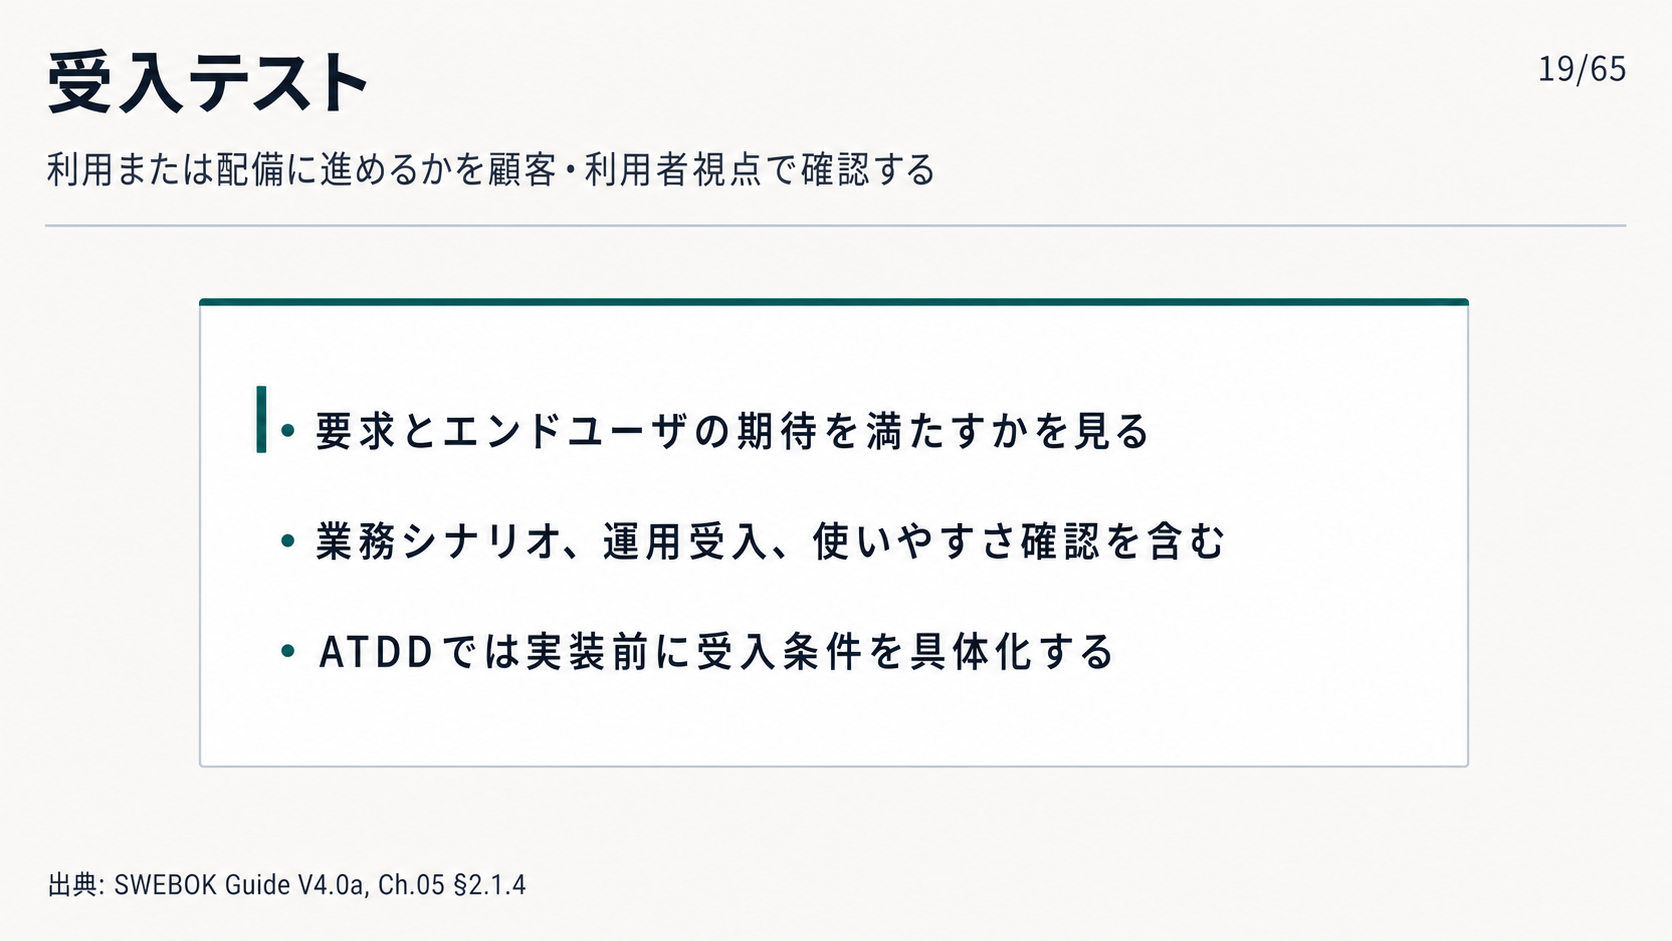
\includegraphics[width=0.96\linewidth]{assets/generated_figures/ch04/fig-ch04-12.png}}{\fbox{\parbox[c][48mm][c]{0.9\linewidth}{\centering 画像生成待ち\\分散・クラウド構築の概念図}}}
\caption{分散・クラウド構築の概念図}
\label{fig:ch04-12}
\end{figure}

\subsubsection{異種システムの構築}

異種システムとは、種類の異なる計算単位が組み合わさったシステムである。GPU、デジタル信号処理プロセッサ、マイクロコントローラ、周辺プロセッサなどが含まれる。組込みシステムは、異種システムであることが多い。

異種システムでは、ハードウェアとソフトウェアを同時に設計する必要がある。これをハードウェア/ソフトウェア協調設計という。複数の仕様言語、複数のシミュレーション環境、インタフェースの整合、共同検証が課題になる。FPGA や ASIC を使ったハードウェア側の試作・実装と、ソフトウェア側の低水準言語への変換が並行して進むことがある。

\subsubsection{性能分析とチューニング}

性能は、アーキテクチャ、詳細設計、データ構造、アルゴリズム、コードの書き方に影響される。性能分析は、プログラムの実行時情報を集め、時間がかかっている箇所、頻繁に実行される箇所、資源を多く使う箇所を見つける活動である。

コードチューニングは、コードレベルで性能を改善することである。論理式、ループ、データ変換、関数呼び出し、メモリアクセスなどを見直す。重要なのは、推測ではなく測定に基づいて行うことである。測定せずに最適化すると、本当に遅い場所ではない箇所を複雑にしてしまう危険がある。

\begin{keybox}{性能改善の原則}
まず測定し、ボトルネックを特定し、小さく変更し、再測定する。性能のために可読性を大きく下げる場合は、その理由と測定結果を残す必要がある。
\end{keybox}

\begin{figure}[htbp]
\centering
\IfFileExists{assets/generated_figures/ch04/fig-ch04-13.png}{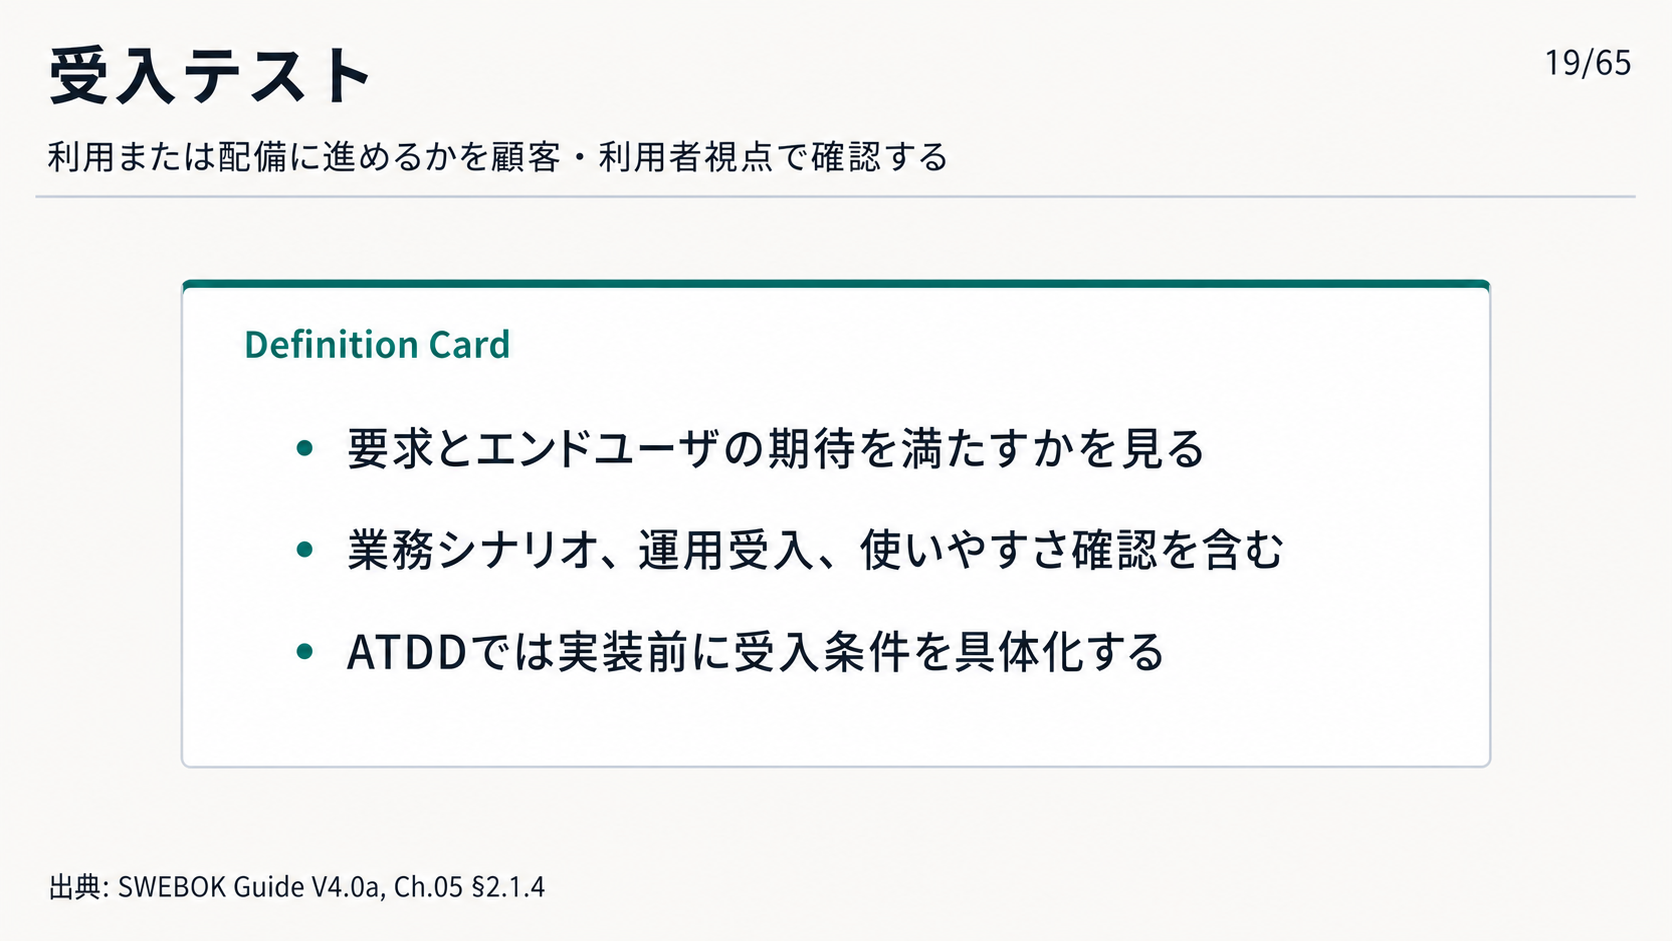
\includegraphics[width=0.96\linewidth]{assets/generated_figures/ch04/fig-ch04-13.png}}{\fbox{\parbox[c][48mm][c]{0.9\linewidth}{\centering 画像生成待ち\\性能分析とチューニングの流れ}}}
\caption{性能分析とチューニングの流れ}
\label{fig:ch04-13}
\end{figure}

\subsubsection{プラットフォーム標準}

プラットフォーム標準は、互換性のある環境でアプリケーションを変更なしに実行しやすくするための標準である。標準サービスや API を定めることで、開発者は特定環境に過度に依存しないアプリケーションを作りやすくなる。

代表例には、エンタープライズ向けの Jakarta Enterprise Edition、Unix 系オペレーティングシステムのインタフェース標準である POSIX、Web アプリケーションの標準を支える HTML5 がある。

標準に従うことは、移植性、相互運用性、保守性を高める。一方で、標準だけでは解決できないプラットフォーム固有の差もあるため、現実の環境での検証が必要である。

\subsubsection{テストファーストプログラミング}

テストファーストプログラミングは、コードを書く前にテストケースを書く開発スタイルである。現在のコードベースでそのテストは失敗する。その後、テストが通るようにコードを書く。テストが通ったら、必要に応じてリファクタリングし、設計を整える。

この方法は、テスト駆動開発としても知られる。テストを先に書くことで、プログラマは要求と設計を先に考える。これにより、要求や設計の問題が早く表面化する。欠陥も早く発見され、修正しやすい。

\begin{figure}[htbp]
\centering
\IfFileExists{assets/generated_figures/ch04/fig-ch04-14.png}{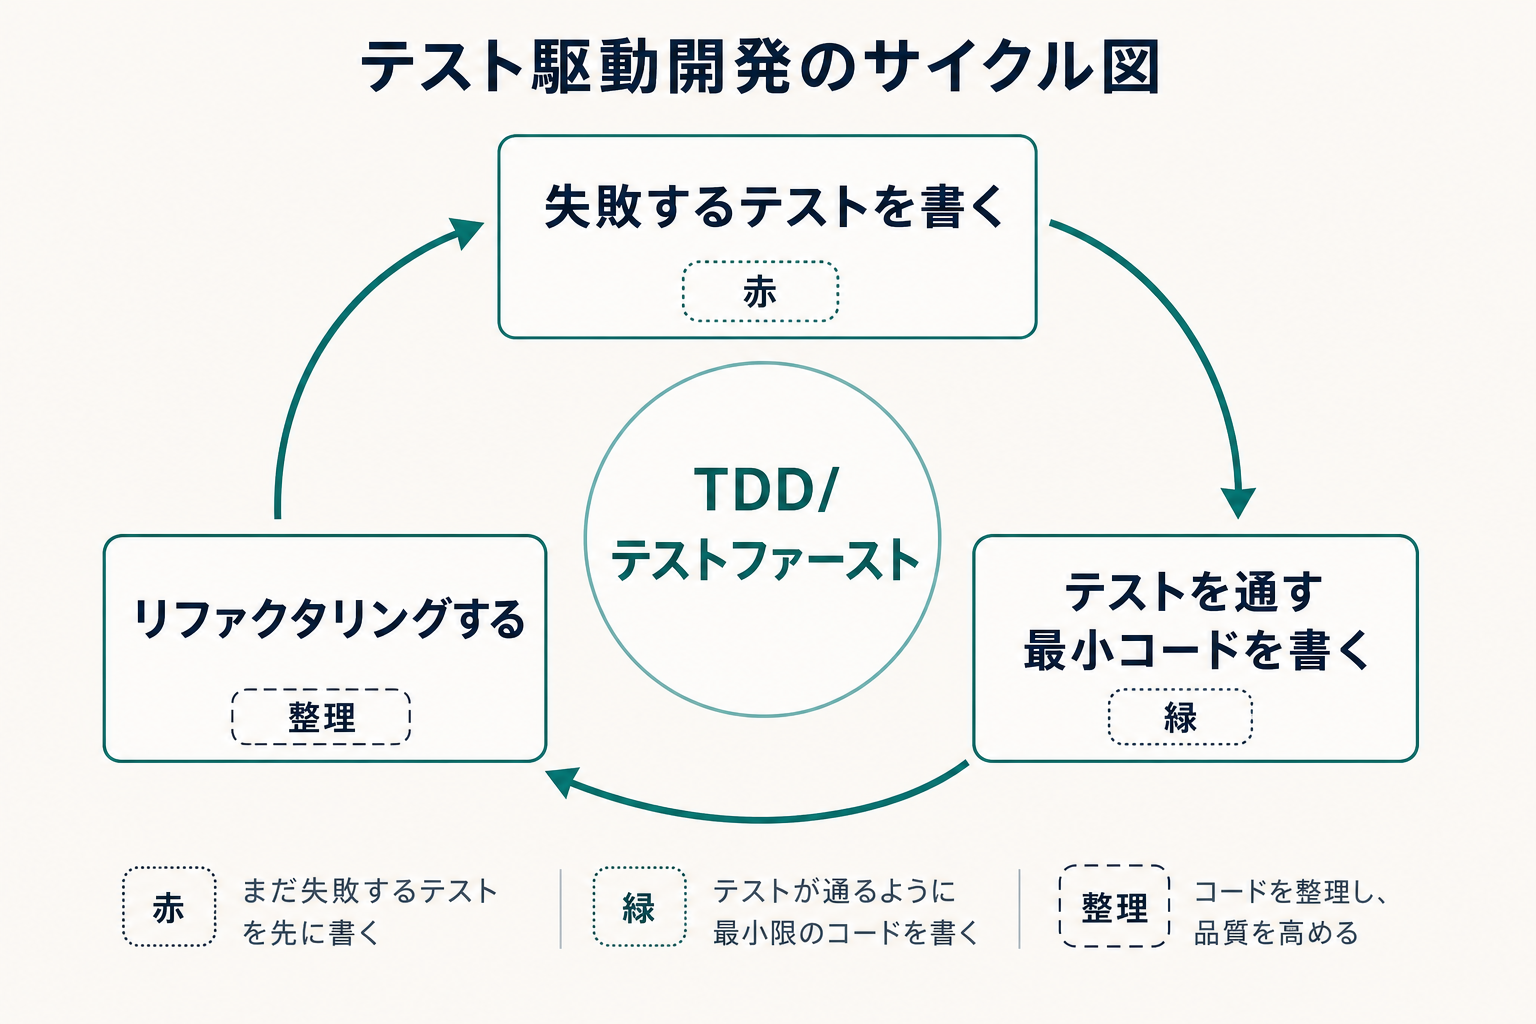
\includegraphics[width=0.96\linewidth]{assets/generated_figures/ch04/fig-ch04-14.png}}{\fbox{\parbox[c][48mm][c]{0.9\linewidth}{\centering 画像生成待ち\\テスト駆動開発のサイクル図}}}
\caption{テスト駆動開発のサイクル図}
\label{fig:ch04-14}
\end{figure}

\subsubsection{構築のためのフィードバックループ}

構築で重要なのは、早く継続的なフィードバックを得ることである。アジャイル開発では、短い反復で動くソフトウェアを作り、顧客やチームから反応を得る。DevOps では、運用環境からの情報を開発へ戻すことで、実際の性能、信頼性、利用状況を学ぶ。

フィードバックループを支える技法には、自動ビルド、自動テスト、継続的統合、カナリアリリース、A/B テスト、監視、ログ分析がある。カナリアリリースは、全利用者に公開する前に、一部の利用者や環境へ変更を出して問題を観察する方法である。A/B テストは、複数の方式を比較し、実利用のデータから判断する方法である。

\subsection{ソフトウェア構築ツール}

構築ツールは、開発者がコードを書き、ビルドし、テストし、デバッグし、性能を測り、問題を発見するための支援を行う。ツールは生産性だけでなく品質にも影響する。ただし、ツールは判断を置き換えるものではない。ツールの結果をどう解釈し、どう改善につなげるかが重要である。

\subsubsection{開発環境}

開発環境、特に統合開発環境は、コード編集、コンパイル、エラー検出、ソースコード管理、ビルド、テスト、デバッグ、リファクタリング支援などを統合する。開発環境の選択は、構築効率と品質に影響する。

近年は、クラウド上の開発環境も使われる。クラウド開発環境では、ブラウザから開発でき、コンテナ化されたビルドやデプロイを利用できることがある。また、大規模言語モデルを使った AI 支援プログラミングも広がっている。AI はコード候補を生成できるが、開発者は生成されたコードをレビューし、テストし、プロジェクトへ適切に統合する責任を持つ。

\subsubsection{視覚的プログラミングとローコード/ゼロコードプラットフォーム}

視覚的プログラミングは、図形や部品を画面上で操作してプログラムを作る方法である。GUI ビルダーは、画面部品をドラッグアンドドロップで配置し、イベント処理のコード生成を支援する。

ローコード/ゼロコードプラットフォームは、視覚的な操作を中心にアプリケーションを作る環境である。ローコードは少量の手書きコードを必要とする。ゼロコードは、原則として手書きコードをほとんど必要としない。これらは、モデル駆動設計、視覚的プログラミング、コード生成の考え方に基づく。

このような環境は、開発速度を高める可能性がある。一方で、複雑な要件、性能、セキュリティ、拡張性、ベンダ依存、テスト容易性には注意が必要である。

\subsubsection{単体テストツール}

単体テストツールは、関数、クラス、モジュールなどを独立して検証するための環境を提供する。テストケースをコードとして記述し、テストランナーが自動で実行し、失敗したテストを報告する。

単体テストツールは、継続的統合と組み合わせることで価値が高まる。開発者が変更を統合するたびにテストを実行すれば、問題を早く発見できる。テストは、回帰を防ぐ安全網にもなる。

\subsubsection{プロファイリング、性能分析、スライシングツール}

プロファイリングツールは、実行中のプログラムを監視し、各文や関数がどれだけ実行されたか、どれだけ時間を使ったかを記録する。これにより、性能上のホットスポットを見つけられる。

プログラムスライシングは、ある変数や処理結果に影響し得る文の集合を計算する技法である。デバッグ、プログラム理解、最適化分析に役立つ。静的解析や動的解析を使ってスライスを求めるツールがある。

\begin{figure}[htbp]
\centering
\IfFileExists{assets/generated_figures/ch04/fig-ch04-15.png}{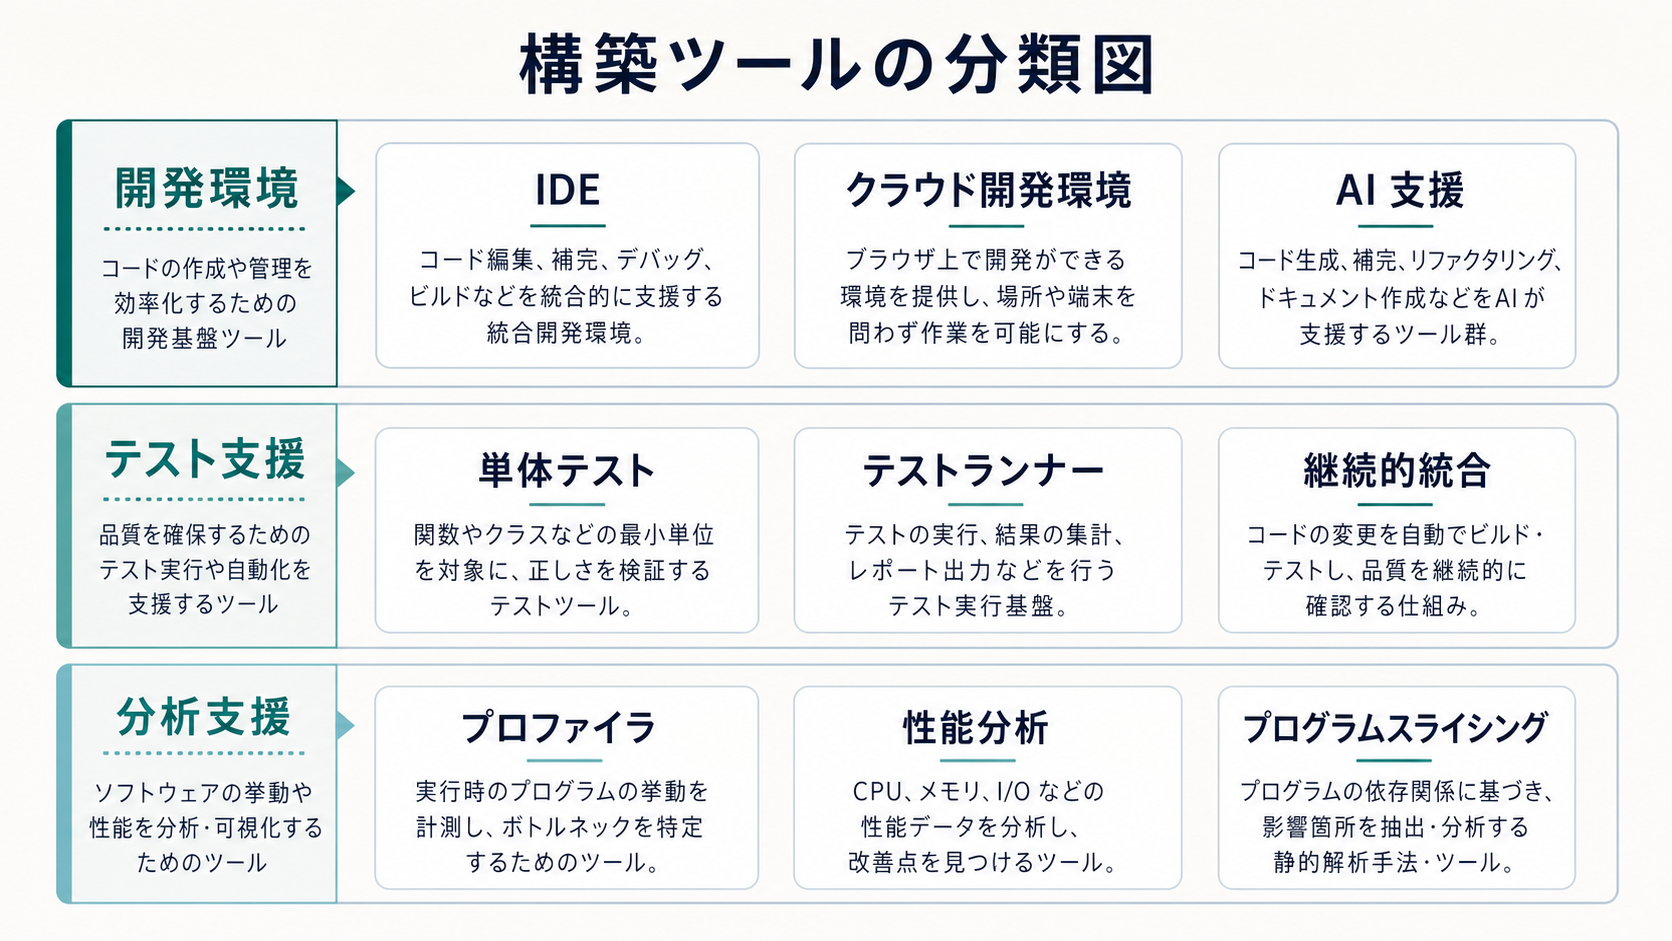
\includegraphics[width=0.96\linewidth]{assets/generated_figures/ch04/fig-ch04-15.png}}{\fbox{\parbox[c][48mm][c]{0.9\linewidth}{\centering 画像生成待ち\\構築ツールの分類図}}}
\caption{構築ツールの分類図}
\label{fig:ch04-15}
\end{figure}

\subsection{トピックと参考文献の対応}

この表は、SWEBOK が示すトピック対参考資料の行列を、学習用に簡略化したものである。詳しく学ぶときは、各トピックに対応する文献を読む。

\par\smallskip\noindent\refstepcounter{table}\label{tab:ch04-04}\textbf{表 \thetable: 第04章 ソフトウェア構築 表04}\par\smallskip
\begin{longtable}{L{0.46\linewidth}L{0.46\linewidth}}
\toprule
\textbf{トピック} & \textbf{主な参考資料} \\
\midrule
1. ソフトウェア構築の基礎 & McConnell, \textit{Code Complete}; Sommerville, \textit{Software Engineering}; Kim et al., \textit{The DevOps Handbook} \\
1.1 複雑さの最小化 & McConnell \\
1.2 変化を予期し受け入れる & McConnell; Sommerville; Kim et al. \\
1.3 検証しやすく構築する & McConnell \\
1.4 資産の再利用 & Sommerville \\
1.5 構築における標準の適用 & McConnell \\
2. 構築の管理 & McConnell; Sommerville; Kim et al. \\
2.1 ライフサイクルモデルにおける構築 & McConnell; Sommerville; Kim et al. \\
2.2 構築計画 & McConnell \\
2.3 構築測定 & McConnell \\
2.4 依存関係の管理 & Sommerville \\
3. 実務上の考慮 & McConnell; Sommerville; Heitkötter et al. \\
3.1 構築設計 & McConnell; Sommerville \\
3.2 構築言語 & McConnell \\
3.3 コーディング & McConnell \\
3.4 構築テスト & McConnell; Sommerville \\
3.5 構築における再利用 & Sommerville \\
3.6 構築品質 & McConnell; Sommerville \\
3.7 統合 & McConnell; Sommerville; Kim et al. \\
3.8 クロスプラットフォーム開発と移行 & Heitkötter et al. \\
4. 構築技術 & McConnell; Sommerville; Clements et al.; Gamma et al.; Mellor and Balcer; Null and Lobur; Silberschatz et al. \\
4.1 API の設計と利用 & Clements et al. \\
4.2 オブジェクト指向の実行時問題 & McConnell \\
4.3 パラメータ化、テンプレート、総称 & Gamma et al. \\
4.4 表明、契約による設計、防御的プログラミング & McConnell \\
4.5 エラー処理、例外処理、フォールトトレランス & McConnell \\
4.6 実行可能モデル & Mellor and Balcer \\
4.7 状態に基づく構築技法と表駆動構築技法 & McConnell \\
4.8 実行時設定と国際化 & McConnell \\
4.9 文法に基づく入力処理 & McConnell; Null and Lobur \\
4.10 並行処理の基本部品 & Silberschatz et al. \\
4.11 ミドルウェア & Clements et al.; Null and Lobur \\
4.12 分散およびクラウド基盤ソフトウェアの構築方法 & Sommerville; Kim et al. \\
4.13 異種システムの構築 & Null and Lobur \\
4.14 性能分析とチューニング & McConnell \\
4.15 プラットフォーム標準 & Heitkötter et al.; Null and Lobur; Silberschatz et al. \\
4.16 テストファーストプログラミング & McConnell; Sommerville \\
4.17 構築のためのフィードバックループ & Kim et al. \\
5. ソフトウェア構築ツール & McConnell; Sommerville \\
5.1 開発環境 & McConnell \\
5.2 視覚的プログラミングとローコード/ゼロコード & McConnell \\
5.3 単体テストツール & McConnell; Sommerville \\
5.4 プロファイリング、性能分析、スライシングツール & McConnell \\
\bottomrule
\end{longtable}

\subsection{発展的な読み物}

\par\smallskip\noindent\refstepcounter{table}\label{tab:ch04-05}\textbf{表 \thetable: 第04章 ソフトウェア構築 表05}\par\smallskip
\begin{longtable}{L{0.34\linewidth}L{0.58\linewidth}}
\toprule
\textbf{文献} & \textbf{読むと得られること} \\
\midrule
McConnell, \textit{Code Complete} & コーディング、複雑さの管理、構築品質、レビュー、テスト、チューニングを実務的に学べる。構築を初めて体系的に学ぶときの中心文献である。 \\
Sommerville, \textit{Software Engineering} & ソフトウェア工学全体の中で、構築、再利用、分散システム、テストを位置づけて理解できる。 \\
Kim et al., \textit{The DevOps Handbook} & 継続的デリバリ、DevOps、フィードバックループ、運用からの学習を学べる。 \\
Fowler and Beck, \textit{Refactoring} & 既存コードの設計を改善し、変更しやすくする具体的な方法を学べる。 \\
Robert C. Martin, \textit{Clean Code} & 読みやすく保守しやすいコードを書くための原則を学べる。 \\
IEEE Std. 1517-2010 & 再利用に基づく開発、再利用のための構築、再利用による構築のプロセスを学べる。 \\
ISO/IEC 12207 & ソフトウェアライフサイクルプロセス全体の中で、構築、統合、再利用を位置づけられる。 \\
\bottomrule
\end{longtable}

\subsection{参考文献}

\begin{enumerate}
  \item S. McConnell, \textit{Code Complete}, 2nd edition, Microsoft Press, 2004.
  \item I. Sommerville, \textit{Software Engineering}, 10th edition, Addison-Wesley, 2016.
  \item G. Kim et al., \textit{The DevOps Handbook: How to Create World-Class Agility, Reliability and Security in Technology Organizations}, 2nd edition, IT Revolution, 2021.
  \item H. Heitkötter, S. Hanschke, and T. A. Majchrzak, ``Evaluating Cross-Platform Development Approaches for Mobile Applications,'' 2013.
  \item P. Clements et al., \textit{Documenting Software Architectures: Views and Beyond}, 2nd edition, Pearson Education, 2010.
  \item E. Gamma et al., \textit{Design Patterns: Elements of Reusable Object-Oriented Software}, Addison-Wesley Professional, 1994.
  \item S. J. Mellor and M. J. Balcer, \textit{Executable UML: A Foundation for Model-Driven Architecture}, Addison-Wesley, 2002.
  \item L. Null and J. Lobur, \textit{The Essentials of Computer Organization and Architecture}, 5th edition, Jones and Bartlett Publishers, 2018.
  \item A. Silberschatz et al., \textit{Operating System Concepts}, 8th edition, Wiley, 2008.
  \item IEEE Std. 1517-2010, \textit{IEEE Standard for Information Technology - Software Life Cycle Processes - Reuse Processes}.
  \item ISO/IEC 12207, \textit{Systems and Software Engineering - Software Life Cycle Processes}.
  \item M. Fowler and K. Beck, \textit{Refactoring: Improving the Design of Existing Code}, 2nd edition, Addison-Wesley.
  \item R. C. Martin, \textit{Clean Code: A Handbook of Agile Software Craftsmanship}, Pearson Education.
\end{enumerate}

\subsection{章末確認問題}

\begin{enumerate}
  \item ソフトウェア構築は、単なるコーディングとどう違うか。
  \item 複雑さを最小化することが、なぜテストや保守に影響するのか。
  \item 「変化を予期する」と「過剰に柔軟に作る」は何が違うか。
  \item 検証しやすく構築するために、コード構造で注意すべきことを三つ挙げよ。
  \item 再利用のための構築と、再利用による構築の違いを説明せよ。
  \item 構築計画で、部品の統合順序を決めることが重要な理由を説明せよ。
  \item 依存関係管理で、ライセンスと脆弱性を確認すべき理由を説明せよ。
  \item 単体テストと統合テストの違いを説明せよ。
  \item API 設計で「誤用しにくい」ことが重要な理由を説明せよ。
  \item 表明、契約による設計、防御的プログラミングの違いを説明せよ。
  \item 分散・クラウド基盤ソフトウェアで、単一マシンのソフトウェアより難しくなる点を三つ挙げよ。
  \item 性能チューニングで、測定なしに最適化してはならない理由を説明せよ。
\end{enumerate}

\begin{plainbox}
\textbf{解答の方向性}

1 は、構築がコーディング、検証、単体テスト、統合テスト、デバッグ、再利用、統合、依存関係管理などを含む点を述べる。2 は、複雑なコードほど実行経路が多く、理解とテストが難しくなる点を述べる。3 は、予期された変化への備えと、根拠のない過剰設計の違いを述べる。4 以降は、本文の「単純で読みやすいコード」「早いフィードバック」「再利用のリスク」「段階的統合」「契約」「測定に基づく改善」といった語を使って説明できる。
\end{plainbox}

\section{第05章 ソフトウェアテスト}
\begin{pointbox}{この資料の読み方}
専門用語は原則として日本語で示し、必要に応じて英語を括弧内に併記する。英語名は、元資料、試験範囲、ツール名を確認するときの手がかりとして残す。初学者が前提知識なしに読めるように、各節では「何を確認する活動か」「なぜその考え方が必要か」「実務では何に注意するか」を重視する。文体は、だである調に統一する。
\end{pointbox}





\subsection*{全体概要：この章で学ぶこと}
\addcontentsline{toc}{subsection}{全体概要：この章で学ぶこと}
この章は、ソフトウェアテストを「実行による確認」として扱う。テストは、テスト対象システムを動かし、観測された結果と期待される結果を比べる活動である。ただし、現実のソフトウェアでは、すべての入力、すべての状態、すべての環境を試すことはできない。したがって、テストは常に、限られた資源でどのテストケースを選ぶかという判断を伴う。

\begin{pointbox}{到達目標}
この章を読み終えると、次のことができるようになる。
\begin{itemize}[leftmargin=2em]
  \item 欠陥、障害、テストケース、テストスイート、テストオラクルを区別できる。
  \item 単体テスト、結合テスト、システムテスト、受入テストの違いを説明できる。
  \item 仕様ベース、構造ベース、経験ベース、欠陥ベース、利用ベースのテスト技法を比較できる。
  \item カバレッジ、欠陥密度、信頼性成長モデル、ミューテーションスコアなどの測度の役割を説明できる。
  \item テスト計画、設計、環境構築、実行、インシデント報告、完了判断の流れを説明できる。
  \item 従来型開発、アジャイル、DevOps、TDD、クラウド、AI、ブロックチェーンなどでテストがどう変わるかを説明できる。
\end{itemize}
\end{pointbox}

初学者は、まず「テストは何を証明でき、何を証明できないか」を押さえるとよい。次に、テストのレベル、目的、技法を分けて理解する。最後に、測定、プロセス、ツールの話に進むと、個別技法が実務の中でどう使われるかを理解しやすい。

\begin{figure}[htbp]
\centering
\IfFileExists{assets/generated_figures/ch05/fig-ch05-01.png}{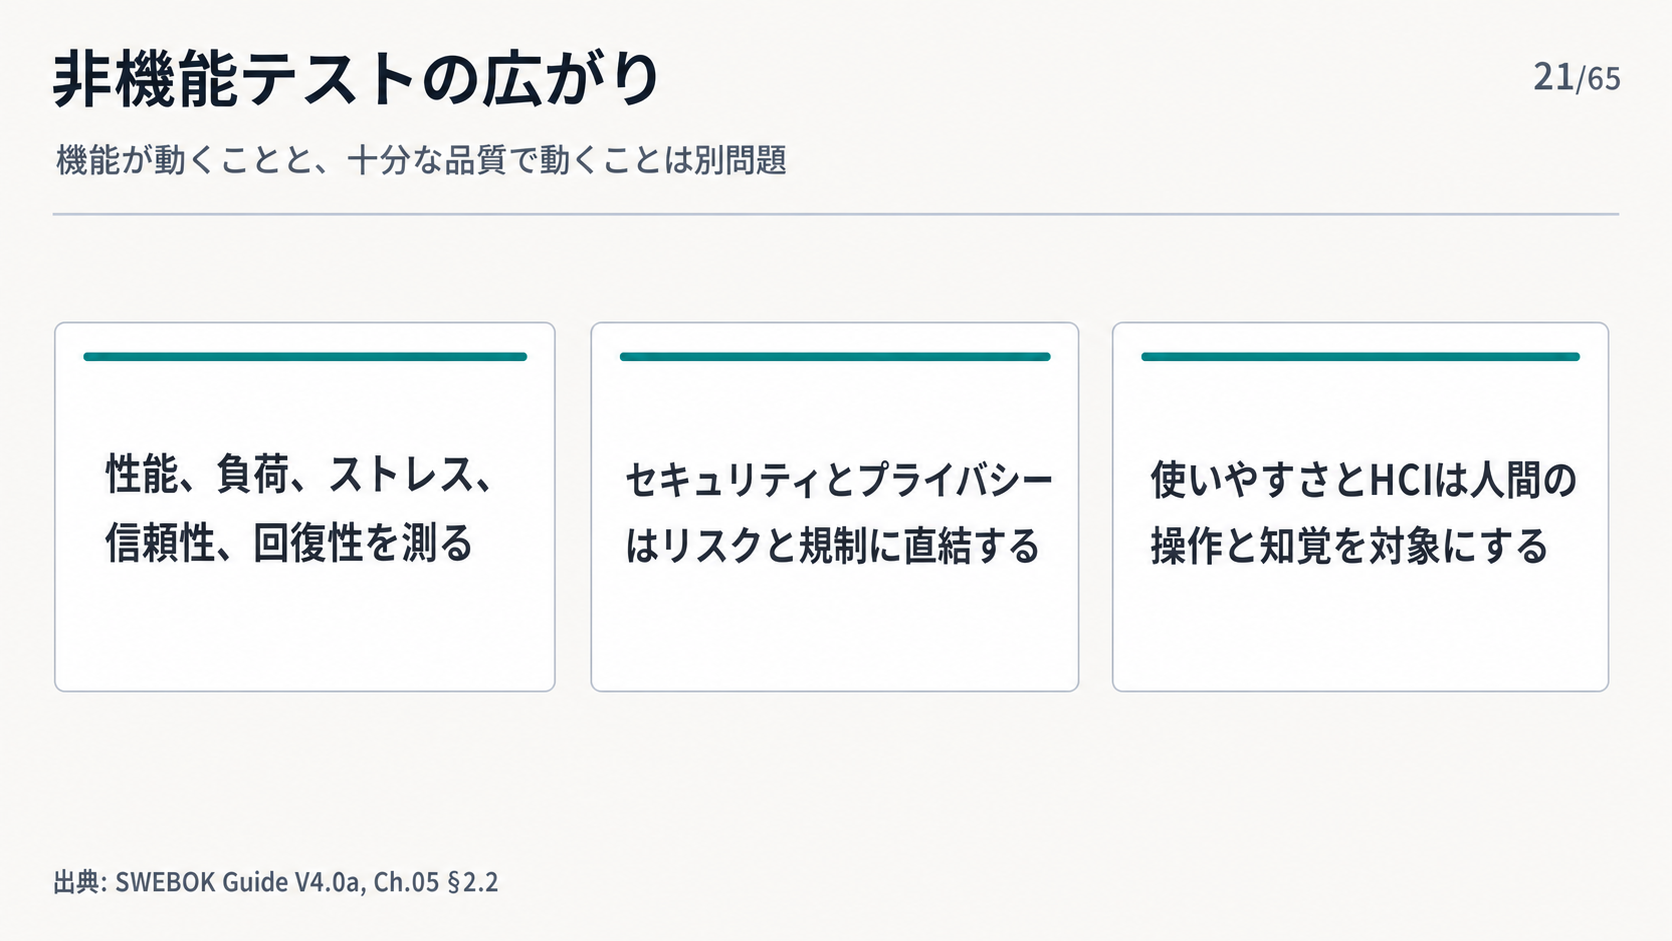
\includegraphics[width=0.96\linewidth]{assets/generated_figures/ch05/fig-ch05-01.png}}{\fbox{\parbox[c][48mm][c]{0.9\linewidth}{\centering 画像生成待ち\\05 章の全体地図}}}
\caption{05 章の全体地図}
\label{fig:ch05-01}
\end{figure}

\subsection*{最初に必要な用語}
\addcontentsline{toc}{subsection}{最初に必要な用語}
\par\smallskip\noindent\refstepcounter{table}\label{tab:ch05-01}\textbf{表 \thetable: 第05章 ソフトウェアテスト 表01}\par\smallskip
\begin{longtable}{P{0.23\linewidth}P{0.69\linewidth}}
\toprule
\textbf{用語} & \textbf{初学者向けの説明} \\
\midrule
テスト対象システム SUT & テストされる対象である。プログラム、アプリケーション、サービス、マイクロサービス、ミドルウェア、システム、システム群、エコシステムまで含み得る。\\
テストケース & 入力値だけでなく、実行条件、時刻条件、手順、期待結果を含む、テスト実行のための具体的な指定である。\\
テストスイート & 複数のテストケースをまとめた集合である。\\
期待結果 & テストを実行したときに、本来得られるべき出力、状態変化、メッセージ、振る舞いである。\\
テストオラクル & 実際の結果が正しいかどうかを判定する基準または仕組みである。人、仕様、モデル、コード注釈、比較ツールなどがなり得る。\\
欠陥 & 障害を引き起こす原因である。コード、設計、要求、設定、運用手順に存在し得る。\\
障害 & 利用者や外部から観測される望ましくない振る舞いである。欠陥が存在しても、条件がそろわなければ障害として現れないことがある。\\
カバレッジ & テストが対象のどの部分をどれだけ通ったかを表す度合いである。文、分岐、条件、要求、状態など、対象は目的によって変わる。\\
回帰テスト & 変更後に、以前できていたことが壊れていないかを再確認するテストである。\\
シフトレフト & テストや品質確認を開発の後半に置くだけでなく、早い段階から行う考え方である。\\
\bottomrule
\end{longtable}

\subsection*{導入：ソフトウェアテストとは何か}
\addcontentsline{toc}{subsection}{導入：ソフトウェアテストとは何か}
ソフトウェアテストとは、通常は無限に近い実行領域から有限個のテストケースを選び、テスト対象システムが期待される振る舞いを提供するかを動的に確認する活動である。この定義には、いくつかの重要な意味が含まれる。

第一に、テストは動的である。つまり、対象を実行して確認する。静的解析、レビュー、形式的証明などは品質向上に重要であるが、この章では主に実行を伴うテストを扱う。

第二に、テストは有限である。すべての入力値、すべての状態、すべての環境を試すことは現実的でない。したがって、テストでは、限られた時間、費用、人員の中で、どのテストケースを選ぶかを決める必要がある。

第三に、テストには期待結果が必要である。実行結果を見ても、それが正しいかどうかを判断できなければテストにならない。期待結果を判断する仕組みがテストオラクルである。

\begin{figure}[htbp]
\centering
\IfFileExists{assets/generated_figures/ch05/fig-ch05-02.png}{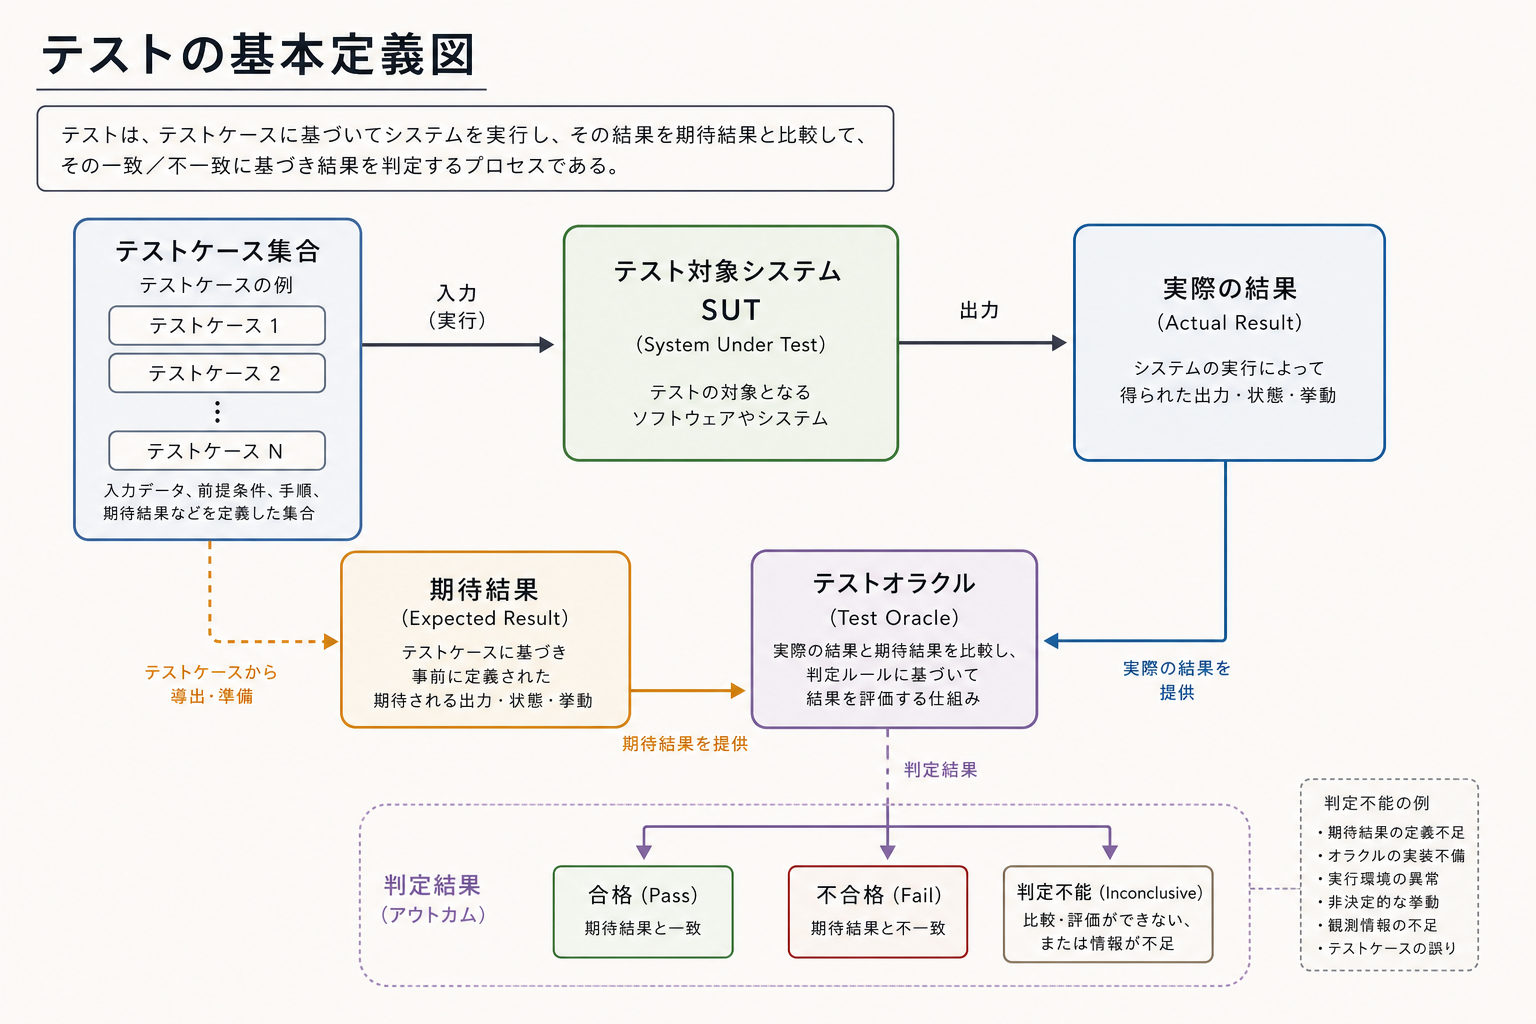
\includegraphics[width=0.96\linewidth]{assets/generated_figures/ch05/fig-ch05-02.png}}{\fbox{\parbox[c][48mm][c]{0.9\linewidth}{\centering 画像生成待ち\\テストの基本定義図}}}
\caption{テストの基本定義図}
\label{fig:ch05-02}
\end{figure}

\subsection{ソフトウェアテストの基礎}
\subsubsection{欠陥と障害}
欠陥は、望ましくない振る舞いの原因である。障害は、その原因が実行時に表に出て、利用者や外部システムから観測される現象である。欠陥があっても、該当する入力や状態に到達しなければ障害として現れないことがある。逆に、障害が観測されても、どの欠陥が原因かを一意に決められるとは限らない。

テストが直接明らかにするのは、多くの場合、障害である。テストに失敗した後は、デバッグや原因分析によって欠陥を見つけ、修正する必要がある。したがって、「テスト」と「デバッグ」は連続して使われることが多いが、同じ活動ではない。テストは失敗を検出する活動であり、デバッグは原因を突き止めて直す活動である。

\begin{pointbox}{重要}
テストは、欠陥の存在を示すことはできるが、欠陥が存在しないことを一般には証明できない。現実のソフトウェアでは、完全な網羅テストが不可能だからである。
\end{pointbox}

\begin{figure}[htbp]
\centering
\IfFileExists{assets/generated_figures/ch05/fig-ch05-03.png}{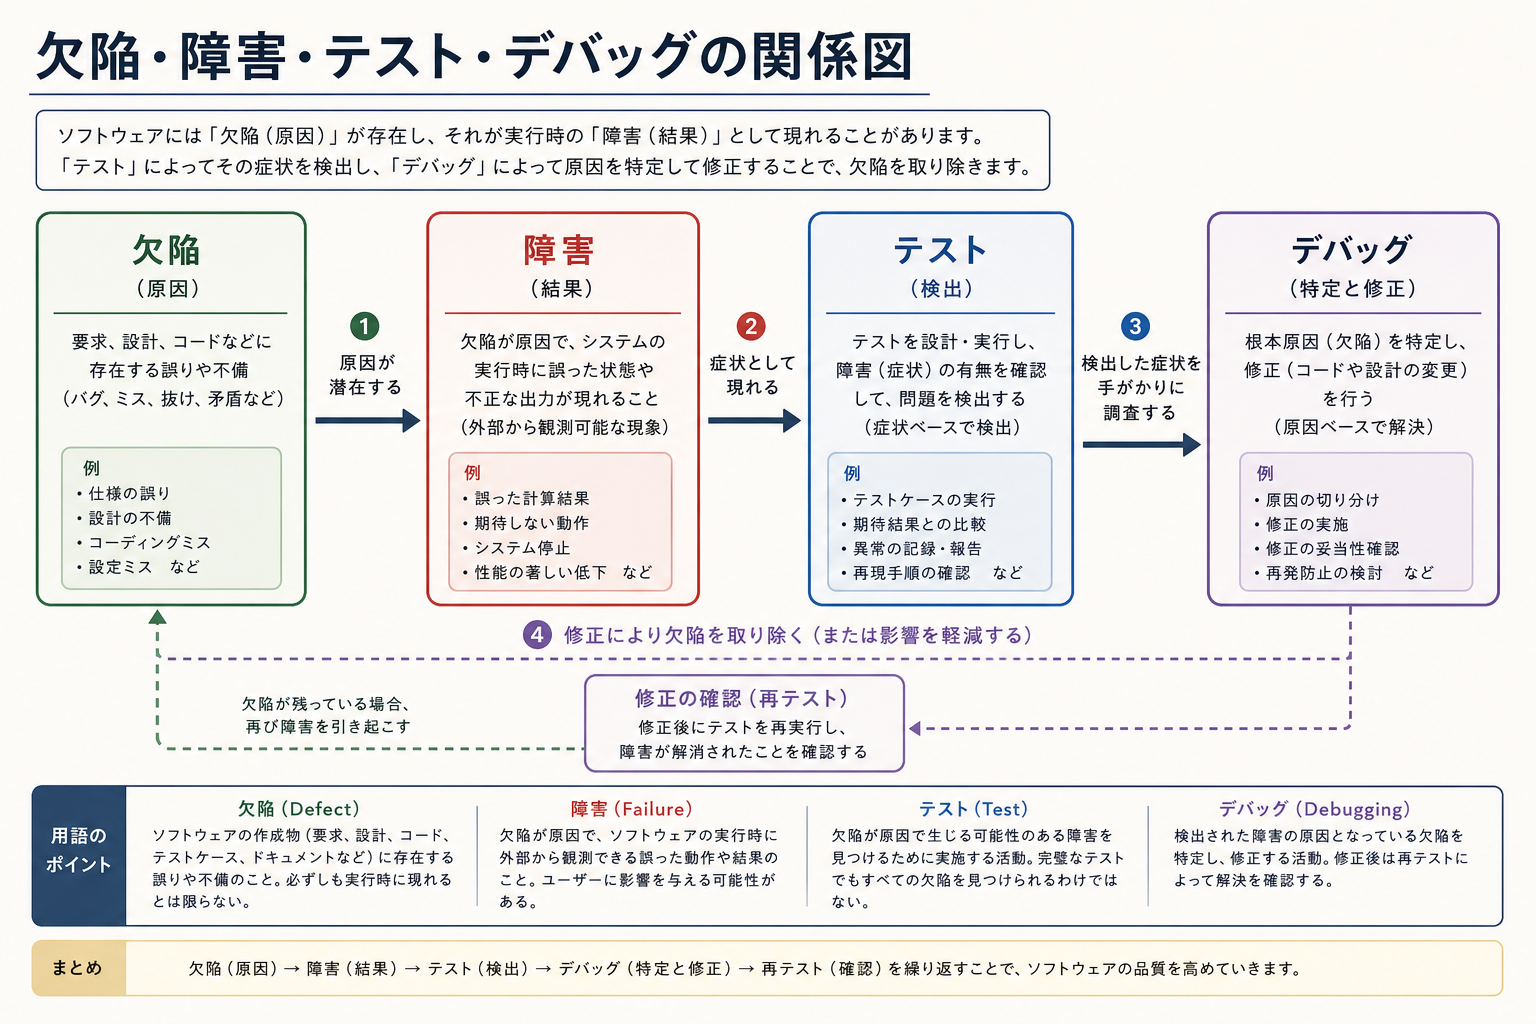
\includegraphics[width=0.96\linewidth]{assets/generated_figures/ch05/fig-ch05-03.png}}{\fbox{\parbox[c][48mm][c]{0.9\linewidth}{\centering 画像生成待ち\\欠陥・障害・テスト・デバッグの関係図}}}
\caption{欠陥・障害・テスト・デバッグの関係図}
\label{fig:ch05-03}
\end{figure}

\subsubsection{主要論点}
\paragraph{テストケース作成}
テストケース作成とは、特定の目的に役立つテストスイートを作る活動である。目的は、十分性の確認、正確性の確認、法令や標準への適合評価などである。テストケース作成は手間が大きいため、自動生成、モデルベース生成、仕様からの導出、コード構造からの導出などの技法やツールが用いられる。

\paragraph{テスト選択と十分性基準}
テスト選択基準は、どのテストケースを選ぶかを決めるための基準である。テスト十分性基準は、どの程度まで実施すれば十分とみなすかを決める基準である。たとえば、全分岐を少なくとも一度通す、すべての機能要求を少なくとも一度検証する、主要なリスクをすべて扱う、などが考えられる。

\paragraph{優先順位付けと最小化}
テストケース優先順位付けは、実行順序を決める活動である。重要度、リスク、過去の欠陥検出率、コードカバレッジ、類似度などを使い、価値の高いテストから先に実行する。テストケース最小化は、冗長なテストケースを削り、テストスイートを小さくする活動である。目的は、効果をできるだけ保ちながら費用と時間を下げることである。

\paragraph{テスト目的}
テストは、目的によって選ぶ技法も評価方法も変わる。機能が仕様どおりかを確認するテスト、性能を測るテスト、セキュリティ上の弱点を探すテスト、利用者が使いやすいかを確認するテストでは、必要なテストケースも期待結果も異なる。目的を曖昧にしたままテストすると、「たくさん実行したが何を確認したかわからない」という状態になりやすい。

\paragraph{評価と認証}
評価や認証のためのテストでは、要求、法令、標準、契約に対する根拠を示す必要がある。テストケースがどの基準から導かれたか、どの構成のシステムで実行されたか、同じ手順で再現できるかが重要である。認証が必要な領域では、テスト結果だけでなく、プロセスや文書の管理も重視される。

\paragraph{品質保証と品質改善のためのテスト}
テストは、品質保証と品質改善にも使われる。品質保証では、要求された品質水準を満たしていることを示す根拠を作る。品質改善では、失敗、欠陥、傾向、弱点を把握し、次の設計、実装、プロセス改善につなげる。

\paragraph{オラクル問題}
オラクル問題とは、実行結果が正しいかどうかを判断することが難しい問題である。期待結果が明確な四則演算なら判断は容易である。しかし、推薦システム、画像認識、複雑な最適化、機械学習モデル、長時間運用システムでは、何を正しい結果とみなすかが難しい。オラクルを自動化することも、しばしば高コストである。

\paragraph{理論的・実践的制約}
テストには限界がある。代表的な限界は、完全な網羅ができないこと、成功したテストが欠陥の不存在を証明しないこと、運用環境を完全には再現できないこと、期待結果を決めるのが難しいこと、テストケースを増やすほど費用が増えることである。

\paragraph{実行不能経路の問題}
実行不能経路とは、制御フロー上は存在するように見えるが、どの入力でも実際には通れない経路である。構造ベーステストでは、経路を通すテストを作ろうとしても、実行不能経路があると達成できない。実行不能経路の特定は、テスト時間の削減やセキュリティ上の弱点分析にも関係する。

\paragraph{テスト容易性}
テスト容易性には二つの意味がある。第一に、対象がテストしやすい構造になっているかである。第二に、欠陥がある場合にテストスイートが障害を露出させやすいかである。観測しにくい内部状態、外部環境に強く依存する処理、再現性の低い並行処理は、テスト容易性を下げる。

\paragraph{テスト実行と自動化}
テスト自動化は、入力生成、実行、結果比較、ログ収集、レポート作成、回帰テストなどを支援する。自動化は有効であるが、すべてを自動化すればよいわけではない。期待結果が曖昧なテスト、探索的な確認、人間の評価が必要な使いやすさの確認では、人手の役割が残る。

\paragraph{拡張性}
拡張性は、負荷、取引数、データ量、利用者数、分散環境の複雑さが増えたときに、ソフトウェアが対応できる能力である。拡張性のテストでは、単に機能が動くかではなく、規模が増えたときの処理能力、安定性、資源使用量を確認する。

\paragraph{テスト有効性}
テスト有効性は、テストが目的にどれだけ役立ったかを表す。欠陥検出率、最初の障害を見つけるまでのテスト数、カバレッジ、信頼性向上、残存リスク低減などで評価される。目的が違えば、有効性の測り方も変わる。

\paragraph{制御可能性・再現性・一般化可能性}
制御可能性は、テスト条件をどの程度制御できるかである。再現性は、別の人が同じ手順で同じ結果を得られるかである。一般化可能性は、あるテスト結果が他の環境、利用者、設定にも当てはまるかである。研究でも実務でも、テスト結果を信頼するにはこの三つが重要である。

\paragraph{オフラインテストとオンラインテスト}
オフラインテストは、外部環境との直接的な相互作用を切り離してテストする。オンラインテストは、実際の利用環境や本番に近い環境と相互作用しながらテストする。オフラインは制御しやすく、オンラインは現実に近い。どちらも期待結果を用いて評価する。

\subsubsection{他の活動との関係}
ソフトウェアテストは、品質管理、形式的検証、デバッグ、プログラム構築、セキュリティ、見積り、法的責任と関係する。しかし、それらと同じではない。レビューや静的解析は実行しない確認であり、テストを補完する。形式的検証は数学的に性質を示す活動であり、テストとは根拠の作り方が異なる。デバッグは、テストで観測された障害の原因を探して直す活動である。

\subsection{テストレベル}
テストレベルは、何を対象にテストするか、どの目的でテストするかによって分けられる。大きなシステムでは、単体、結合、システム、受入という四つの段階で考えると理解しやすい。ただし、これらは開発プロセスを固定するものではなく、どれが常に最重要というものでもない。

\subsubsection{テスト対象}
\paragraph{単体テスト}
単体テストは、個別にテストできる要素を単独で確認する活動である。対象は、関数、クラス、モジュール、コンポーネント、サブシステムなどである。多くの場合、コードを書いた開発者が実施するが、必ずしもそれに限られない。単体テストの目的は、欠陥を早く見つけ、後段の結合やシステムテストに欠陥を持ち込まないことである。

\paragraph{結合テスト}
結合テストは、複数の要素の相互作用を確認する活動である。モジュール間、コンポーネント間、外部システムとのインタフェース、ハードウェアや運用環境とのやり取りが対象になる。上位から下位へ進めるトップダウン、下位から上位へ進めるボトムアップ、混合方式、一度に結合するビッグバン方式などがある。

\paragraph{システムテスト}
システムテストは、システム全体の振る舞いを確認する活動である。単体テストと結合テストで多くの欠陥は見つかっているはずだが、システム全体で初めて現れる問題もある。機能だけでなく、セキュリティ、プライバシー、速度、正確性、信頼性などの非機能要求の確認にも適している。

\paragraph{受入テスト}
受入テストは、システムが要求とエンドユーザの期待を満たし、利用または配備に進めるかを確認する活動である。利用者や顧客とともに実施されることが多い。運用受入、使いやすさ確認、業務シナリオ確認などを含む。受け入れテスト駆動開発では、機能を実装する前に受入条件を定義する。

\begin{figure}[htbp]
\centering
\IfFileExists{assets/generated_figures/ch05/fig-ch05-04.png}{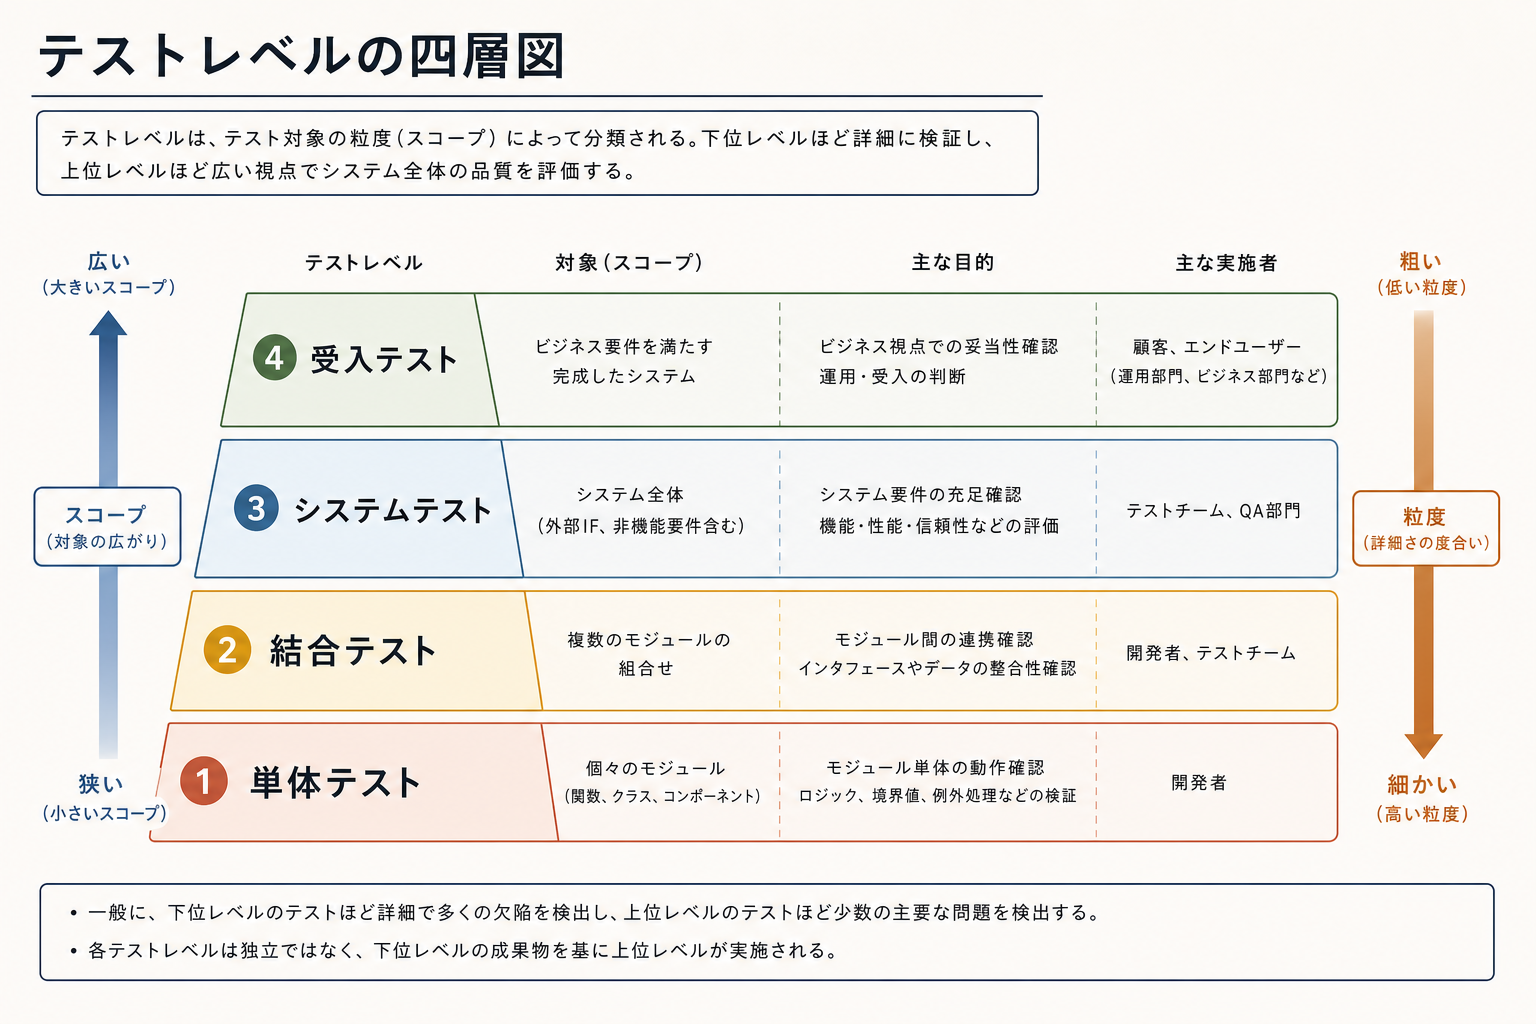
\includegraphics[width=0.96\linewidth]{assets/generated_figures/ch05/fig-ch05-04.png}}{\fbox{\parbox[c][48mm][c]{0.9\linewidth}{\centering 画像生成待ち\\テストレベルの四層図}}}
\caption{テストレベルの四層図}
\label{fig:ch05-04}
\end{figure}

\subsubsection{テスト目的}
テスト目的は、何を確認したいかを表す。目的を明確にすると、テストケースの選び方、測り方、終了判断が決めやすくなる。

\paragraph{適合性テスト}
適合性テストは、SUT が標準、規則、仕様、要求、設計、プロセス、慣行に合っているかを確認する。

\paragraph{法令・規制順守テスト}
法令・規制順守テストは、SUT が法律や規制に従っていることを示す。外部の規制機関や認証制度によって求められることが多い。

\paragraph{導入テスト}
導入テストは、SUT を対象環境へ導入した後に、ハードウェア構成、運用制約、インストール手順を含めて確認する活動である。

\paragraph{アルファテストとベータテスト}
アルファテストは、リリース前に少数の選ばれた利用者に試してもらう活動である。ベータテストは、より広い代表的利用者に試してもらう活動である。いずれも、利用者から問題報告を受けるために行う。

\paragraph{回帰テスト}
回帰テストは、変更後に意図しない悪影響が出ていないことを確認する再テストである。アジャイル、DevOps、テスト駆動開発、継続的開発では特に重要である。すべてのテストを毎回実行するのは高コストなので、選択、最小化、優先順位付けがよく使われる。

\paragraph{優先順位付けテスト}
優先順位付けテストは、テストケースの実行順を工夫し、早い段階で重要な障害を見つけることを狙う。類似していないテストケースから先に実行する類似度ベースの方法などがある。

\paragraph{非機能テスト}
非機能テストは、性能、使いやすさ、信頼性などの非機能面を確認する。代表的な種類を表に示す。

\par\smallskip\noindent\refstepcounter{table}\label{tab:ch05-02}\textbf{表 \thetable: 第05章 ソフトウェアテスト 表02}\par\smallskip
\begin{longtable}{P{0.24\linewidth}P{0.66\linewidth}}
\toprule
\textbf{種類} & \textbf{確認すること} \\
\midrule
性能テスト & 応答時間、処理能力、容量など、性能要求を満たすかを確認する。\\
負荷テスト & 多数の要求や高負荷時に、デッドロック、競合、メモリ漏れ、安定性問題が出ないかを確認する。\\
ストレステスト & 想定を超える負荷を与え、限界や破綻の仕方を確認する。\\
容量テスト & 内部保存容量、データ交換量、情報量に対する限界を確認する。\\
フェイルオーバーテスト & 障害や高負荷時にも、予備資源や代替経路でサービスを継続できるかを確認する。\\
信頼性テスト & 運用プロファイルなどを用いて、将来の信頼性を評価する。\\
互換性テスト & 異なるハードウェア、ソフトウェア、バージョン、リリースと協調できるかを確認する。\\
拡張性テスト & 利用者数、取引数、データ量が増えた場合に対応できるかを確認する。\\
弾力性テスト & クラウドなどで、計算資源、記憶資源、保存資源を増減しても能力を保てるかを確認する。\\
インフラテスト & インフラ構成要素を確認し、停止時間を減らし性能を改善する。\\
バックツーバックテスト & 複数の実装や版に同じ入力を与え、出力差を分析する。\\
回復テスト & クラッシュや災害後に再起動・復旧できるかを確認する。\\
\bottomrule
\end{longtable}

\paragraph{セキュリティテスト}
セキュリティテストは、外部攻撃から SUT とデータを守れるかを確認する。主に機密性、完全性、可用性を扱う。誤用や悪用に対してシステムがどう振る舞うかを確認する負のテストも重要である。

\paragraph{プライバシーテスト}
プライバシーテストは、利用者の個人データを安全に扱い、情報共有方針やプライバシー方針を守れているかを確認する。

\paragraph{インタフェースおよび API テスト}
インタフェーステストは、コンポーネント間でデータや制御情報が正しく交換されるかを確認する。API テストでは、エンドユーザのアプリケーションが API を呼び出す状況を想定し、パラメータ、環境条件、内部データを組み合わせて確認する。

\paragraph{構成テスト}
構成テストは、複数の利用者、環境、設定に対応するソフトウェアが、指定された構成で正しく動くかを確認する。

\paragraph{使いやすさと人間コンピュータ相互作用テスト}
使いやすさテストは、エンドユーザがソフトウェアを学び、使い、誤りから回復できるかを確認する。機能、文書、画面、操作手順、エラー回復が対象になる。

\begin{figure}[htbp]
\centering
\IfFileExists{assets/generated_figures/ch05/fig-ch05-05.png}{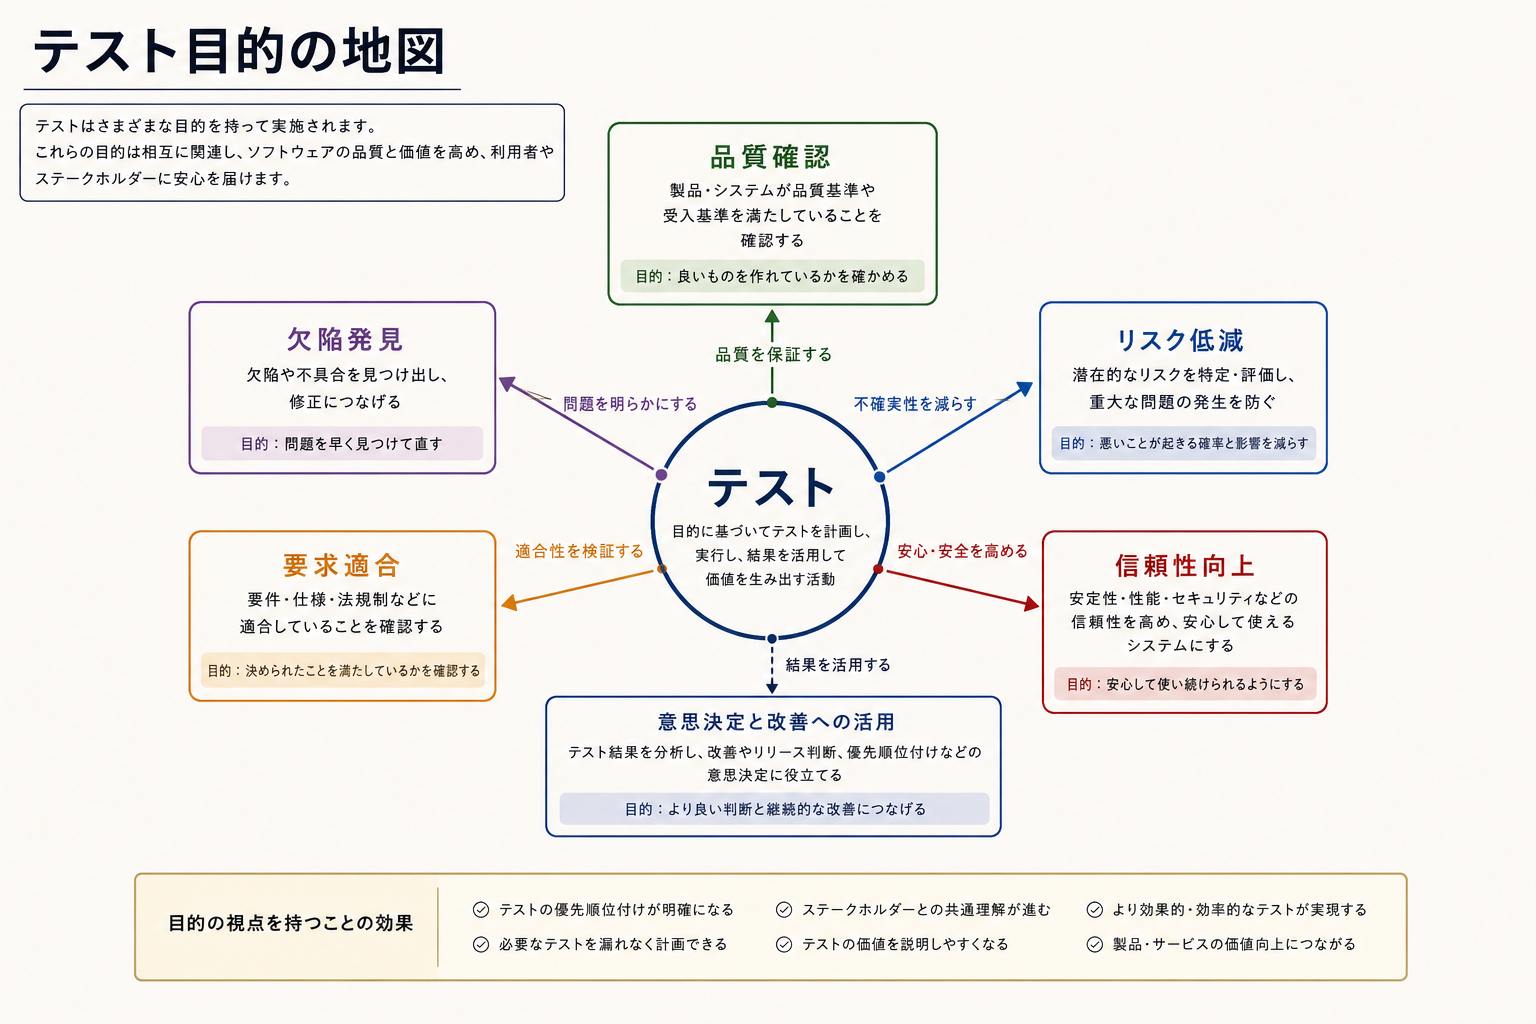
\includegraphics[width=0.96\linewidth]{assets/generated_figures/ch05/fig-ch05-05.png}}{\fbox{\parbox[c][48mm][c]{0.9\linewidth}{\centering 画像生成待ち\\テスト目的の地図}}}
\caption{テスト目的の地図}
\label{fig:ch05-05}
\end{figure}

\subsection{テスト技法}
テスト技法は、テストケースをどの考え方で選ぶかを定める。代表的には、仕様から選ぶ仕様ベース技法、内部構造から選ぶ構造ベース技法、経験から選ぶ経験ベース技法がある。さらに、欠陥モデル、利用モデル、アプリケーションの性質、他領域から得た知識に基づく技法もある。

\begin{figure}[htbp]
\centering
\IfFileExists{assets/generated_figures/ch05/fig-ch05-06.png}{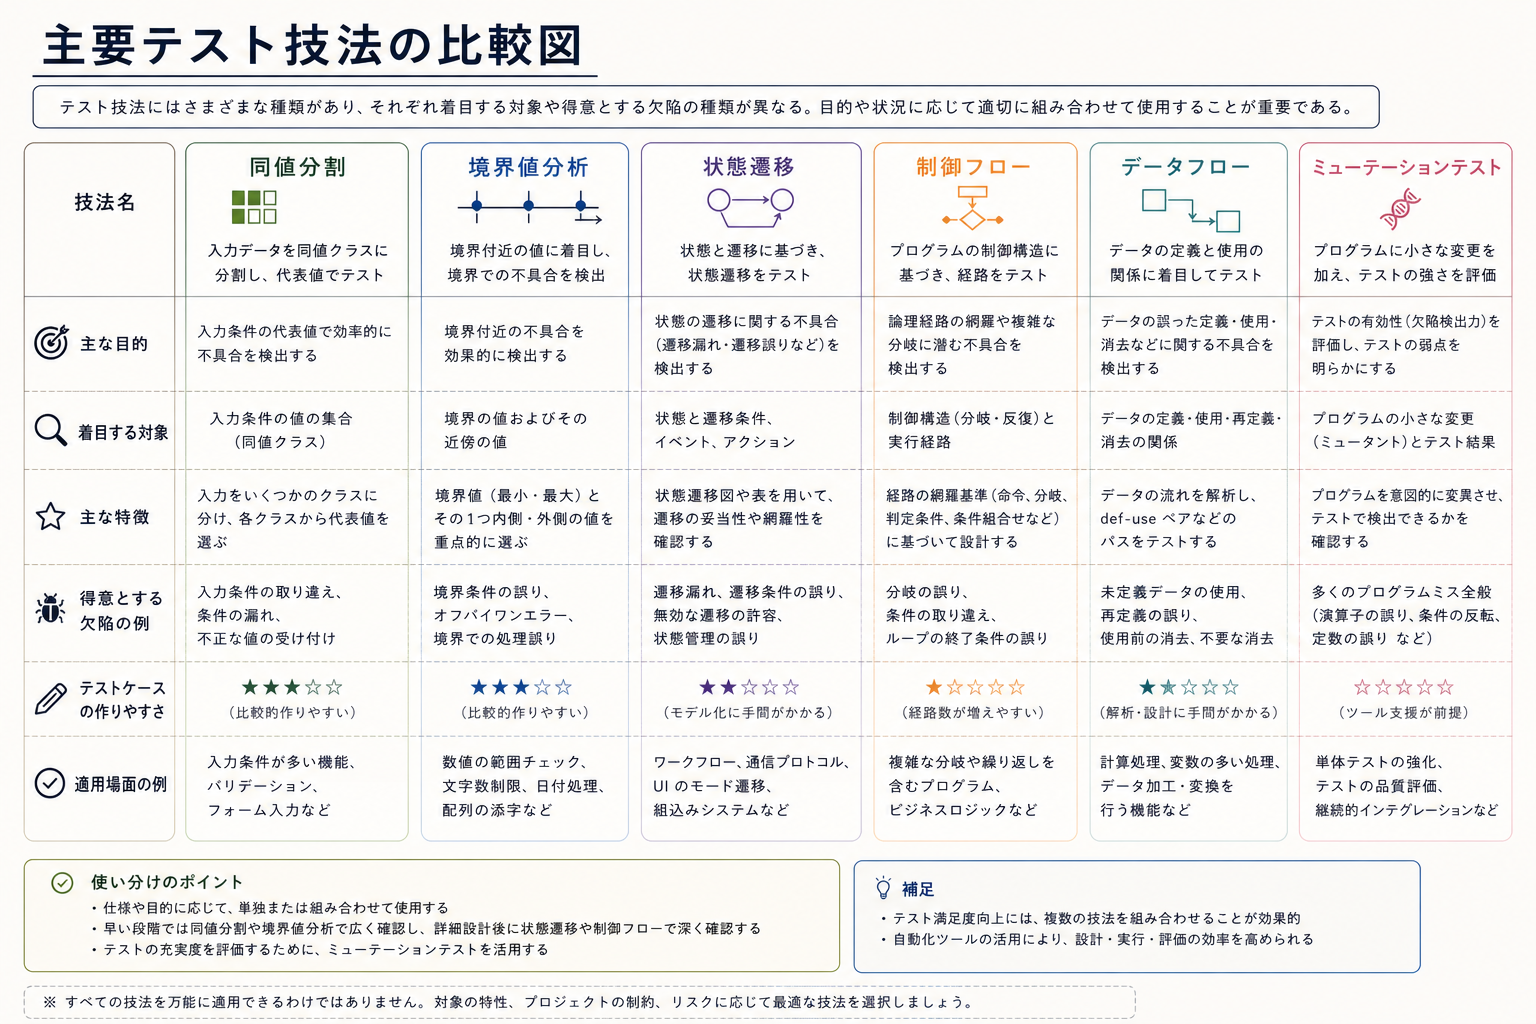
\includegraphics[width=0.96\linewidth]{assets/generated_figures/ch05/fig-ch05-06.png}}{\fbox{\parbox[c][48mm][c]{0.9\linewidth}{\centering 画像生成待ち\\主要テスト技法の比較図}}}
\caption{主要テスト技法の比較図}
\label{fig:ch05-06}
\end{figure}

\subsubsection{仕様ベース技法}
仕様ベース技法は、SUT の入力と出力、要求、仕様、モデルに基づいてテストケースを選ぶ。内部コードを知らなくても使えるため、ブラックボックス技法とも呼ばれる。

\paragraph{同値分割}
同値分割は、入力領域を同じように扱えると考えられる部分集合に分け、各集合から代表値を選ぶ技法である。たとえば、年齢が 0 から 120 まで有効なら、有効範囲、下限未満、上限超過などに分ける。目的は、無数の入力を少数の代表例に縮約することである。

\paragraph{境界値分析}
境界値分析は、入力範囲の境界付近に欠陥が集中しやすいという経験に基づき、下限、上限、その直前直後を選ぶ技法である。範囲外の値を使って堅牢性を見る場合もある。

\begin{figure}[htbp]
\centering
\IfFileExists{assets/generated_figures/ch05/fig-ch05-07.png}{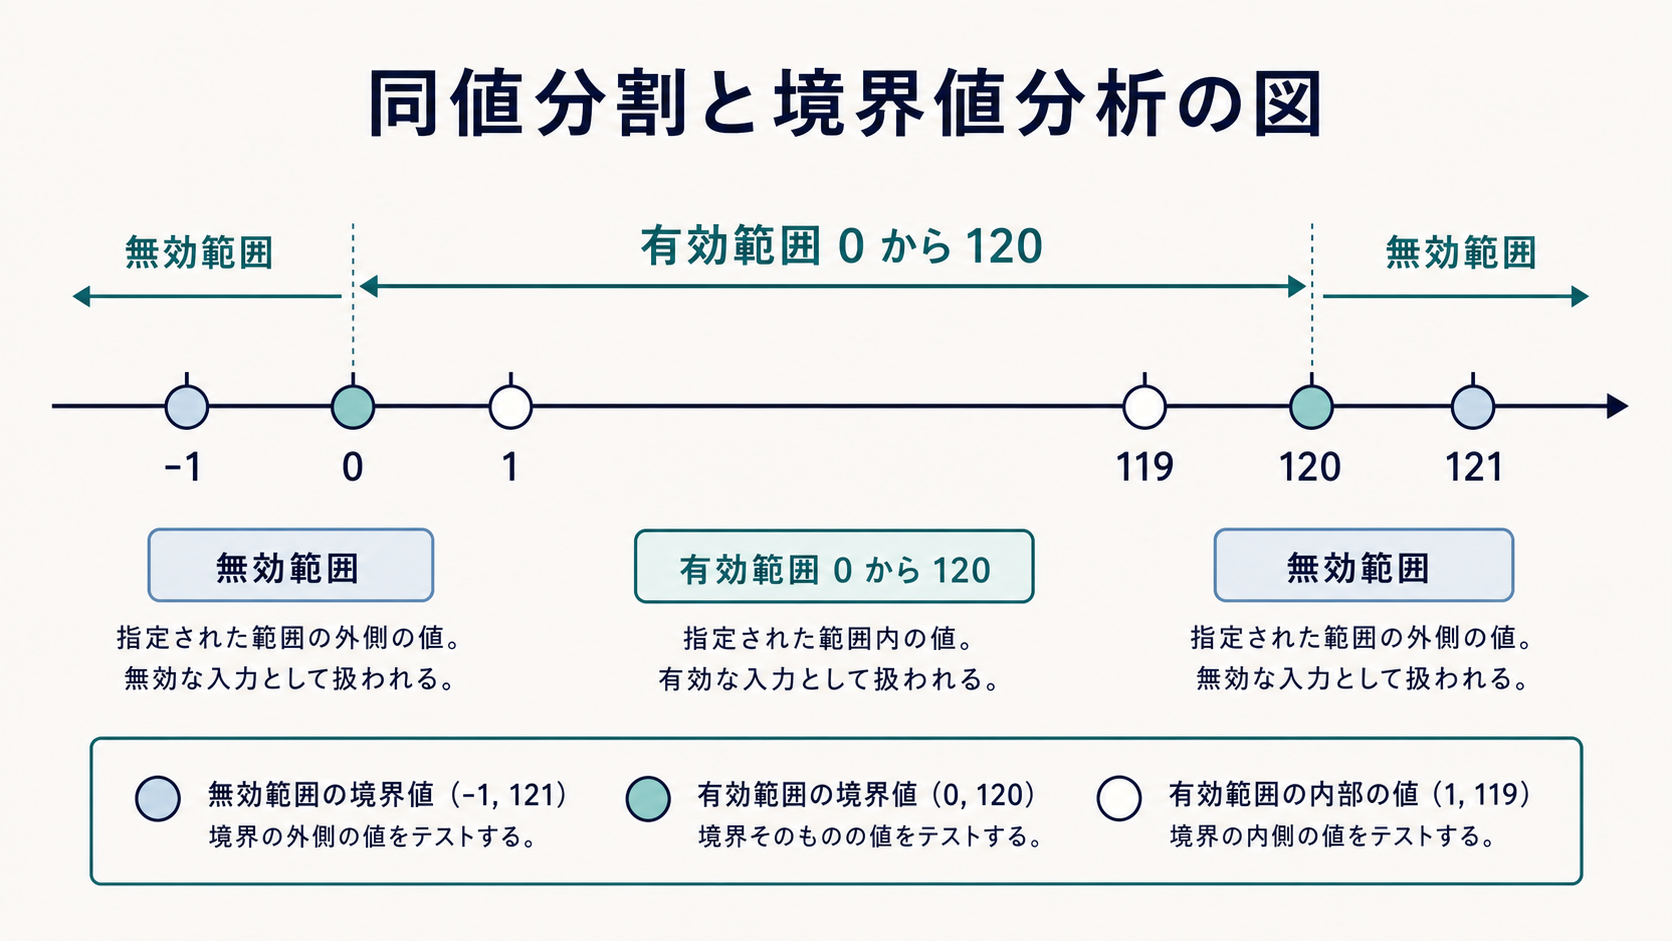
\includegraphics[width=0.96\linewidth]{assets/generated_figures/ch05/fig-ch05-07.png}}{\fbox{\parbox[c][48mm][c]{0.9\linewidth}{\centering 画像生成待ち\\同値分割と境界値分析の図}}}
\caption{同値分割と境界値分析の図}
\label{fig:ch05-07}
\end{figure}

\paragraph{構文テスト}
構文テストは、形式言語で書かれた仕様や入力文法に基づいてテストケースを導く技法である。仕様が形式的であれば、機能テストケースの自動生成や期待結果の判定に使いやすい。

\paragraph{組合せテスト技法}
組合せテストは、入力値や条件の組合せを体系的に選ぶ技法である。すべての組合せを試すと数が爆発するため、ペアワイズテストのように、任意の二つのパラメータの組合せはすべて含めるという基準を使うことが多い。

\paragraph{決定表}
決定表は、条件と動作の組合せを表にして、論理関係を明示する技法である。複数条件によって結果が変わる業務規則に向いている。各条件組合せからテストケースを導けるため、抜け漏れの発見にも役立つ。

\paragraph{原因結果グラフ}
原因結果グラフは、入力条件である原因と、出力や動作である結果の関係を論理グラフとして表す技法である。仕様分析、入力条件の整理、結果条件の特定に役立つ。

\paragraph{状態遷移テスト}
状態遷移テストは、SUT を有限状態機械として表し、状態と遷移をカバーするようにテストケースを作る技法である。画面遷移、通信プロトコル、注文状態、予約状態など、状態によって振る舞いが変わる対象に向いている。

\begin{figure}[htbp]
\centering
\IfFileExists{assets/generated_figures/ch05/fig-ch05-08.png}{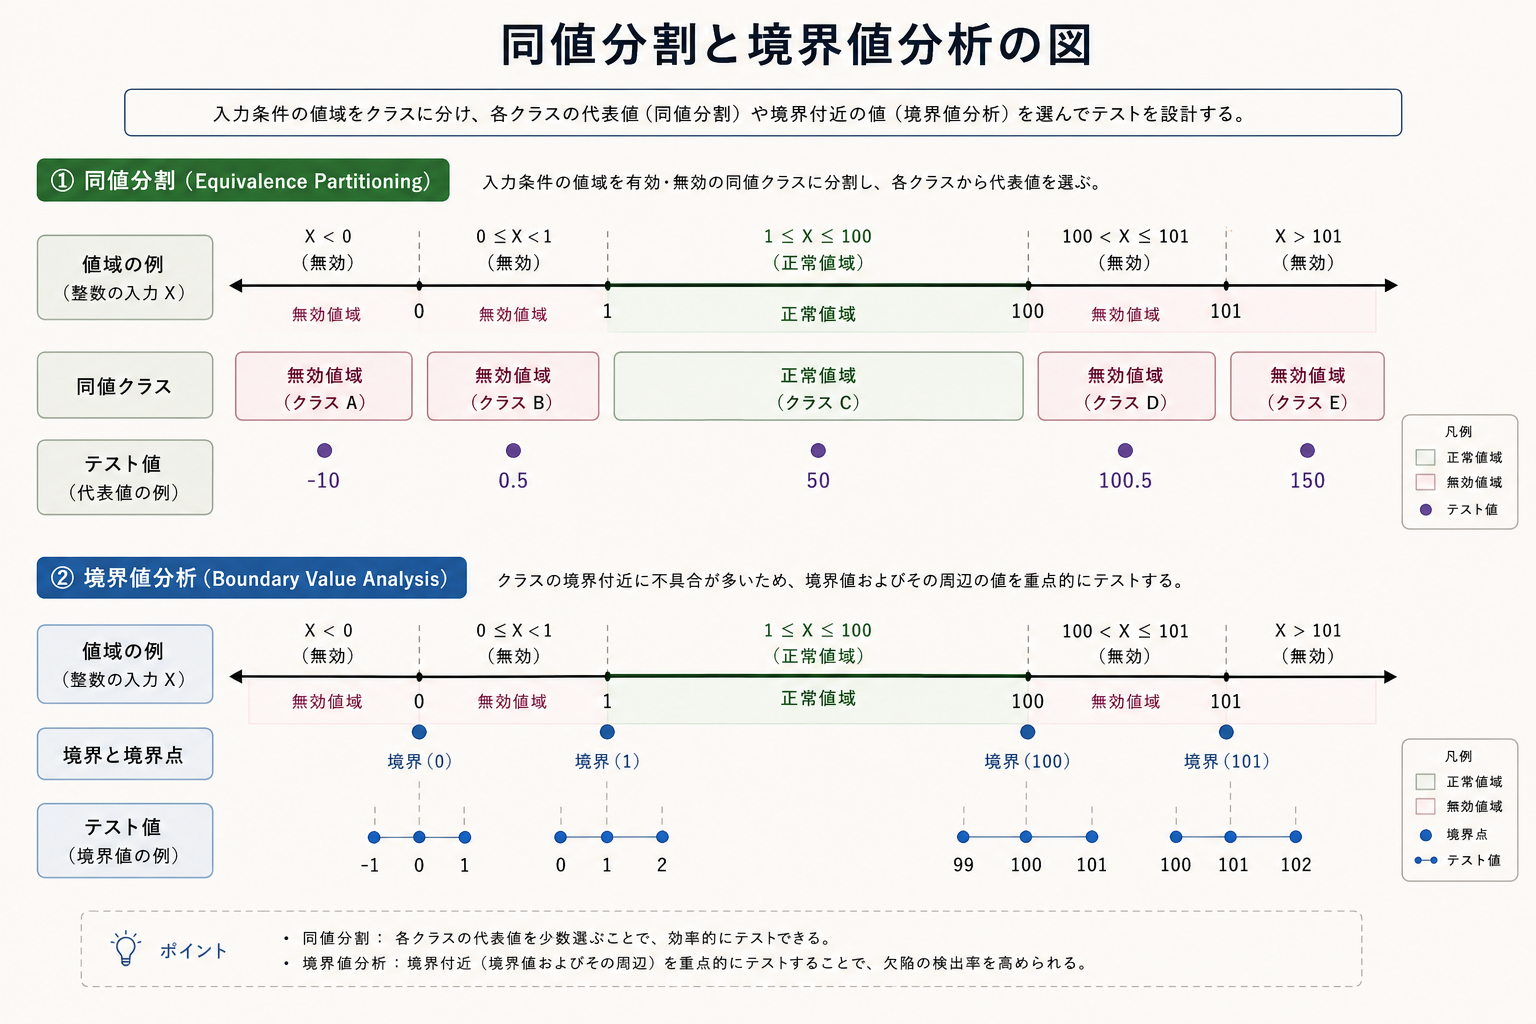
\includegraphics[width=0.96\linewidth]{assets/generated_figures/ch05/fig-ch05-08.png}}{\fbox{\parbox[c][48mm][c]{0.9\linewidth}{\centering 画像生成待ち\\状態遷移テストの図}}}
\caption{状態遷移テストの図}
\label{fig:ch05-08}
\end{figure}

\paragraph{シナリオベーステスト}
シナリオベーステストは、利用者やシステムがたどる一連の行動をモデル化し、その流れに沿ってテストケースを作る技法である。通常の流れだけでなく、代替流、例外流も扱う。業務プロセステストやワークフローモデルを使うテストもこの考え方に含まれる。

\paragraph{ランダムテスト}
ランダムテストは、入力領域からランダムにテストケースを選ぶ技法である。単純な自動化に向いているが、入力領域がわかっている必要がある。不正入力や予期しないデータを大量に与えるファズテストは、セキュリティ分野でよく用いられる。

\paragraph{証拠に基づく技法}
証拠に基づく技法は、厳密な調査手順で得た知見をテストに反映する考え方である。問いを立て、利用できる証拠を集め、批判的に分析する。体系的マッピング研究や体系的レビューは、既存研究や実務知見を整理する手段である。

\paragraph{例外強制テスト}
例外強制テストは、データ例外、操作例外、オーバーフロー、保護例外、アンダーフローなど、あらかじめ決めた例外やエラーを SUT が扱えるかを確認する。多くの場合、負のシナリオを使い、エラーメッセージや回復動作を確認する。

\subsubsection{構造ベーステスト技法}
構造ベース技法は、コードや設計の内部構造を情報源としてテストケースを選ぶ。ホワイトボックス技法とも呼ばれる。文カバレッジ、分岐カバレッジ、経路カバレッジ、循環的複雑度などが関係する。

\paragraph{制御フローテスト}
制御フローテストは、文、分岐、判定、条件、条件組合せ、経路を対象に、どの部分を実行したかを確認する。最も強い基準の一つはすべての入口から出口までの経路を通す経路テストであるが、ループがあると現実的でないため、文カバレッジ、分岐カバレッジ、条件判定カバレッジなどの基準が使われる。

\paragraph{データフローテスト}
データフローテストは、変数の定義、使用、未定義化に注目する。ある変数が定義された後、どの経路でどの使用に届くかを確認する。定義と使用の組合せを扱うため、データに関する隠れた欠陥を見つけやすい。

\paragraph{構造ベース技法の参照モデル}
構造ベース技法では、制御フローグラフがよく使われる。ノードは文や文列を表し、辺は制御の移動を表す。この図に基づいて、どの文、分岐、経路を通したかを可視化できる。

\begin{figure}[htbp]
\centering
\IfFileExists{assets/generated_figures/ch05/fig-ch05-09.png}{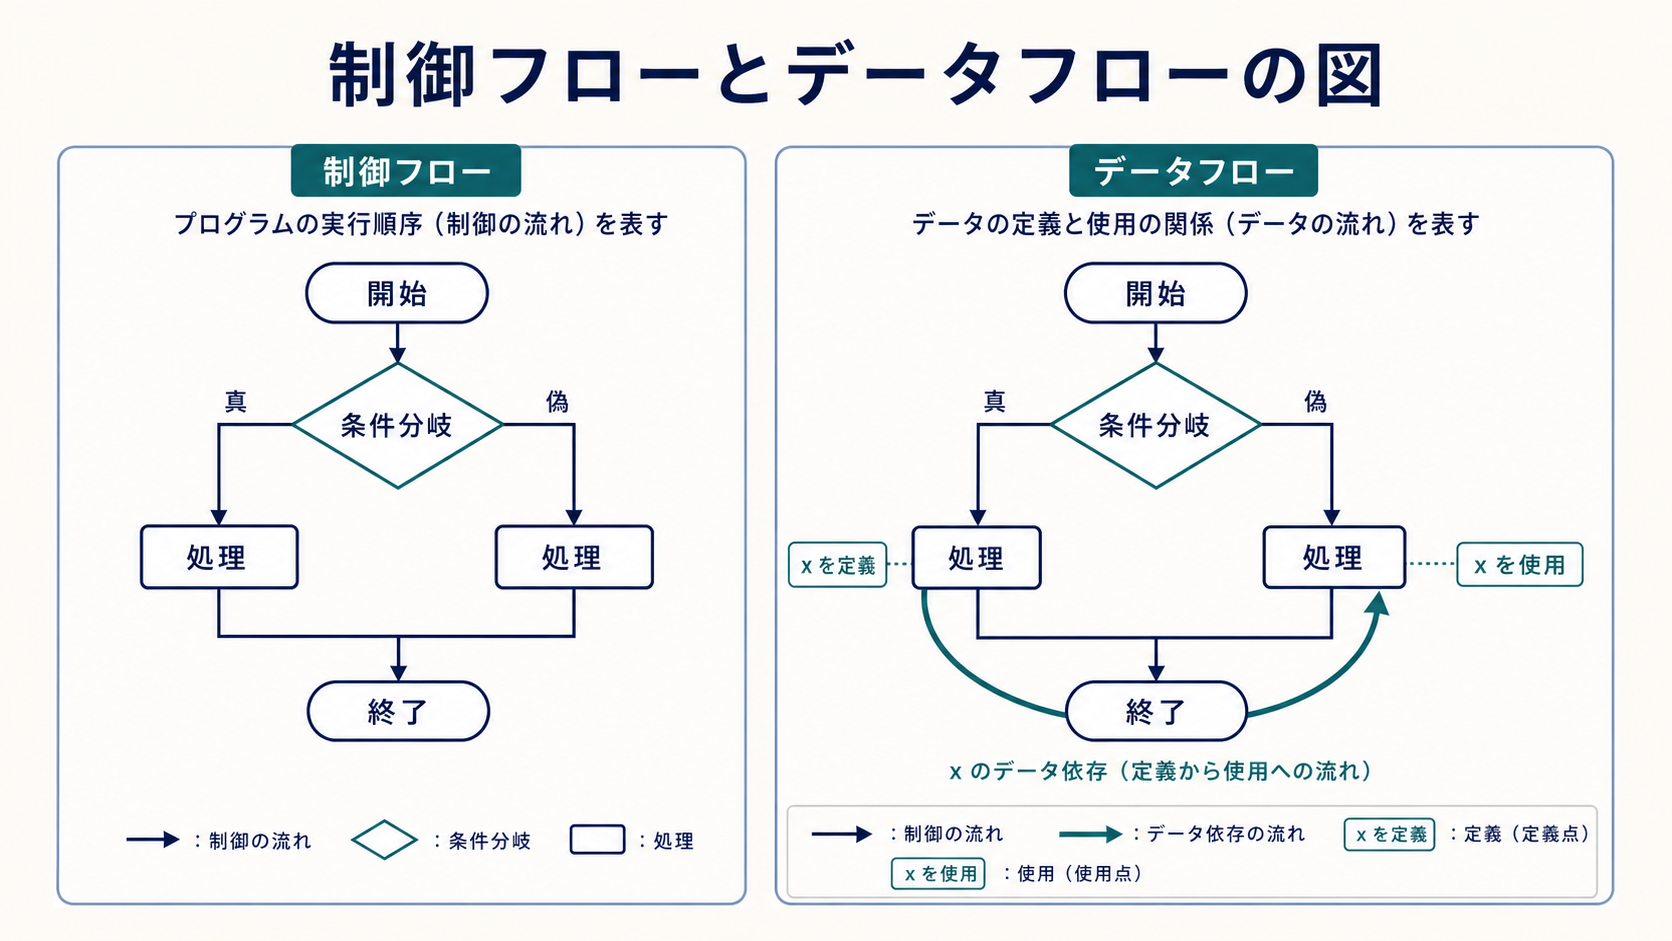
\includegraphics[width=0.96\linewidth]{assets/generated_figures/ch05/fig-ch05-09.png}}{\fbox{\parbox[c][48mm][c]{0.9\linewidth}{\centering 画像生成待ち\\制御フローとデータフローの図}}}
\caption{制御フローとデータフローの図}
\label{fig:ch05-09}
\end{figure}

\subsubsection{経験ベース技法}
経験ベース技法は、仕様やコードだけではなく、テスト担当者の知識、直感、過去の障害、ドメイン理解を活用する。

\paragraph{エラー推測}
エラー推測は、過去の欠陥履歴や経験に基づき、「ここに欠陥がありそうだ」と考えてテストケースを設計する技法である。形式的な技法では見つけにくい問題を見つけることがある。

\paragraph{探索的テスト}
探索的テストは、学習、テスト設計、テスト実行を同時に進める活動である。事前にすべてのテストケースを決めるのではなく、観測した振る舞い、リスク、失敗の兆候に基づいて次のテストを考える。要求が詳細でないアジャイル開発などでよく使われる。

\paragraph{その他の経験ベース技法}
アドホックテストは、技能、直感、経験に基づいてテストする。モンキーテストはランダムな操作で停止や異常を狙う。ペアテストは二人でテストを行い、一人が操作し、一人が観察する。ゲーミフィケーションは、テスト作業をゲーム要素に変換して参加を促す。クイックテストは小さなテストスイートで重大問題を早く見つける。スモークテストは、ビルド後に基本機能が動くかを確認し、本格的なテストに進める状態かを判断する。

\subsubsection{欠陥ベース技法とミューテーション技法}
欠陥ベーステストは、あり得る欠陥の種類を想定し、それを露出させるテストケースを作る。欠陥分類や直交欠陥分類を使うと、欠陥の意味情報を整理し、根本原因分析を短縮できる。

ミューテーションテストは、SUT をわずかに変更した変異体を多数作り、テストスイートがそれらの違いを検出できるかを評価する技法である。テストが変異体を見破れば、その変異体は殺されたという。変異体を多く殺せるテストスイートほど、欠陥検出能力が高いと考える。近年は、機械学習システムのテストで、入力を変化させて出力関係を見るメタモルフィックテストにも関連する。

\begin{figure}[htbp]
\centering
\IfFileExists{assets/generated_figures/ch05/fig-ch05-10.png}{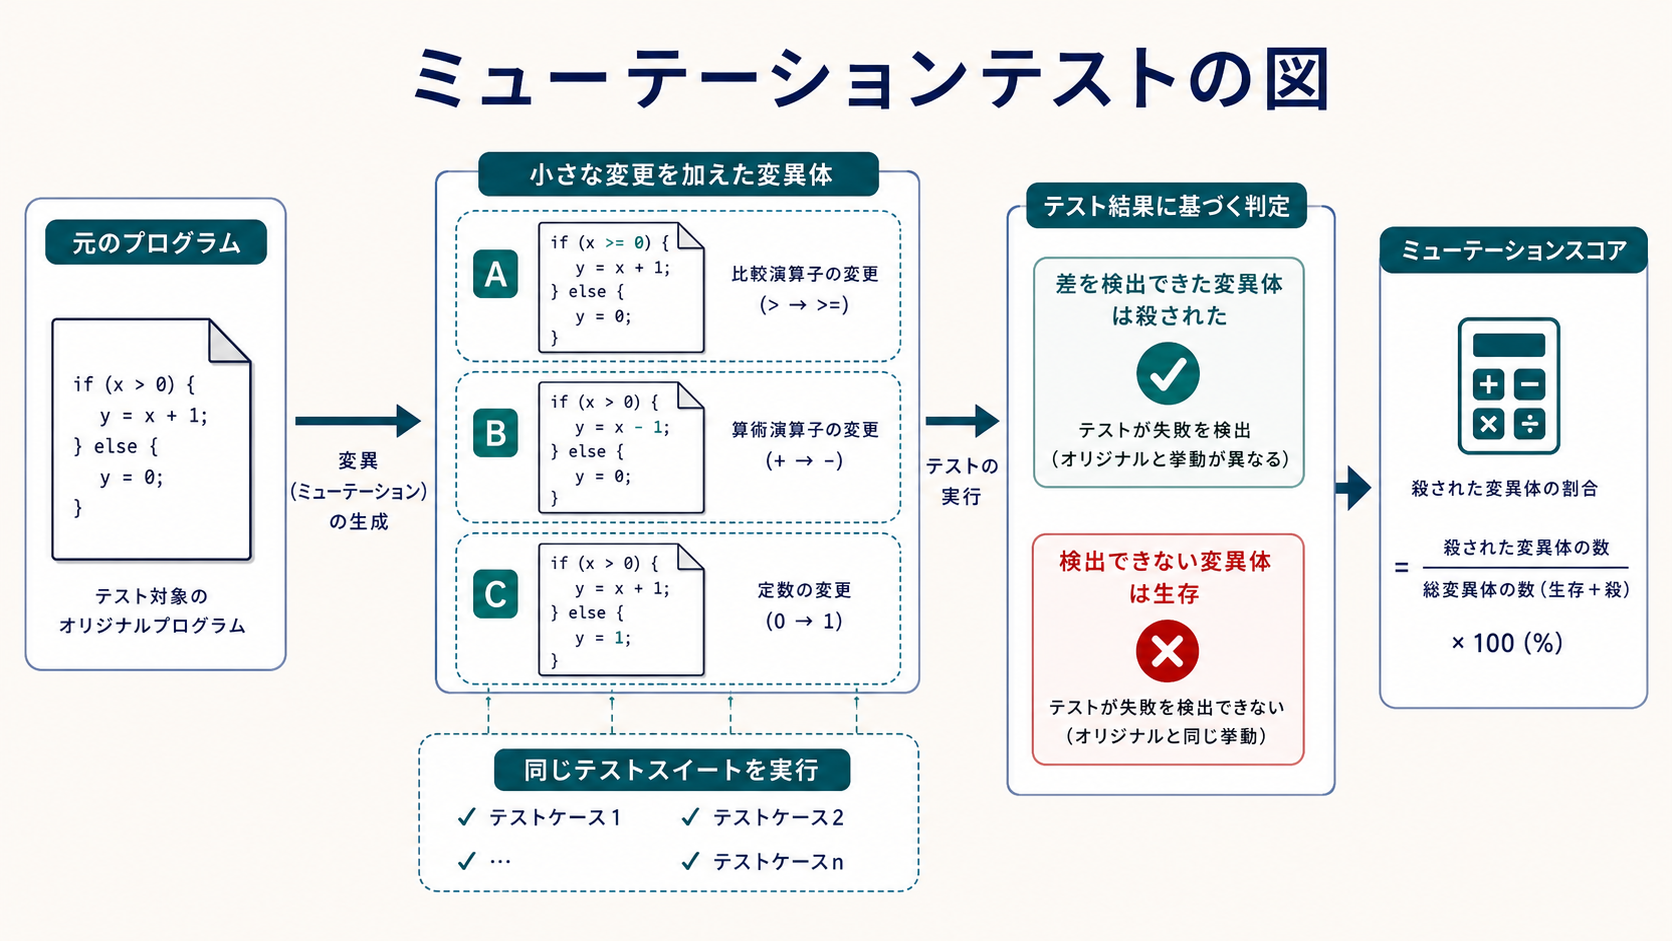
\includegraphics[width=0.96\linewidth]{assets/generated_figures/ch05/fig-ch05-10.png}}{\fbox{\parbox[c][48mm][c]{0.9\linewidth}{\centering 画像生成待ち\\ミューテーションテストの図}}}
\caption{ミューテーションテストの図}
\label{fig:ch05-10}
\end{figure}

\subsubsection{利用ベース技法}
利用ベース技法は、実際の運用や利用のされ方をモデル化し、その頻度や順序に沿ってテストケースを選ぶ。運用環境に近い条件で実行するため、受入テストや信頼性評価に向いている。

\paragraph{運用プロファイル}
運用プロファイルは、入力や利用シナリオが実運用でどの頻度で起こるかを表す。運用プロファイルに基づくテストでは、観測した結果から将来の信頼性を推定する。難しさは、現実的なプロファイルを作ることにある。

\paragraph{利用者観察ヒューリスティック}
利用者観察ヒューリスティックは、利用者がシステムやインタフェースをどれだけうまく使えるかを、統制された条件で観察する。認知的ウォークスルー、発話思考法、現場観察、質問票、面接などが使われる。

\subsubsection{アプリケーションの性質に基づく技法}
一般的な技法は多くのソフトウェアに使えるが、対象の性質によって追加の技法が必要になる。オブジェクト指向ソフトウェア、コンポーネントベースソフトウェア、ウェブアプリケーション、並行プログラム、通信プロトコル、リアルタイムシステム、安全重要システム、サービス指向ソフトウェア、オープンソース、組込み、クラウド、ブロックチェーン、ビッグデータ、AI・機械学習、モバイル、セキュリティ・プライバシー重視ソフトウェアなどでは、対象特有のリスクを考慮する。

\subsubsection{技法の選択と組合せ}
実務では、一つの技法だけで十分な品質根拠を得ることは少ない。仕様ベースと構造ベースを組み合わせれば、外部振る舞いと内部網羅を両方確認できる。リスクが高い部分には手厚い技法を使い、低リスク部分には軽量な技法を使うなど、目的、費用、リスク、組織制約に応じて選ぶ。

\paragraph{機能的技法と構造的技法の組合せ}
シナリオベーステストは機能的観点を強く持つ。構造ベーステストは内部構造の観点を強く持つ。両者は対立ではなく補完関係である。仕様に書かれた動作を確認しつつ、実装上の分岐やデータ流れも確認することで、見落としを減らせる。

\paragraph{決定的テストとランダムテスト}
決定的テストは、基準に従って選ばれたテストケースを実行する。ランダムテストは、確率分布に従って入力を選ぶ。信頼性テストではランダム性が役立つことがあるが、境界や特定リスクを狙う場合には決定的な選択が有効である。

\subsubsection{派生知識に基づく技法}
派生知識に基づく技法は、他の研究領域や文脈から得られた知識をテストに取り入れる。デジタルツイン、シミュレーション、機械学習、ゲーミフィケーション、模擬ニューラルネットワークなどが例である。テスト活動を支援し、効果を高めることを目的とする。

\subsection{テスト関連測度}
測度は、テスト目標が達成されたかを判断するために必要である。テスト技法は道具であり、測度はその道具が目的に役立っているかを判断する根拠である。測度は、テスト計画の最適化、進捗管理、品質分析、完了判断に使われる。

\begin{figure}[htbp]
\centering
\IfFileExists{assets/generated_figures/ch05/fig-ch05-11.png}{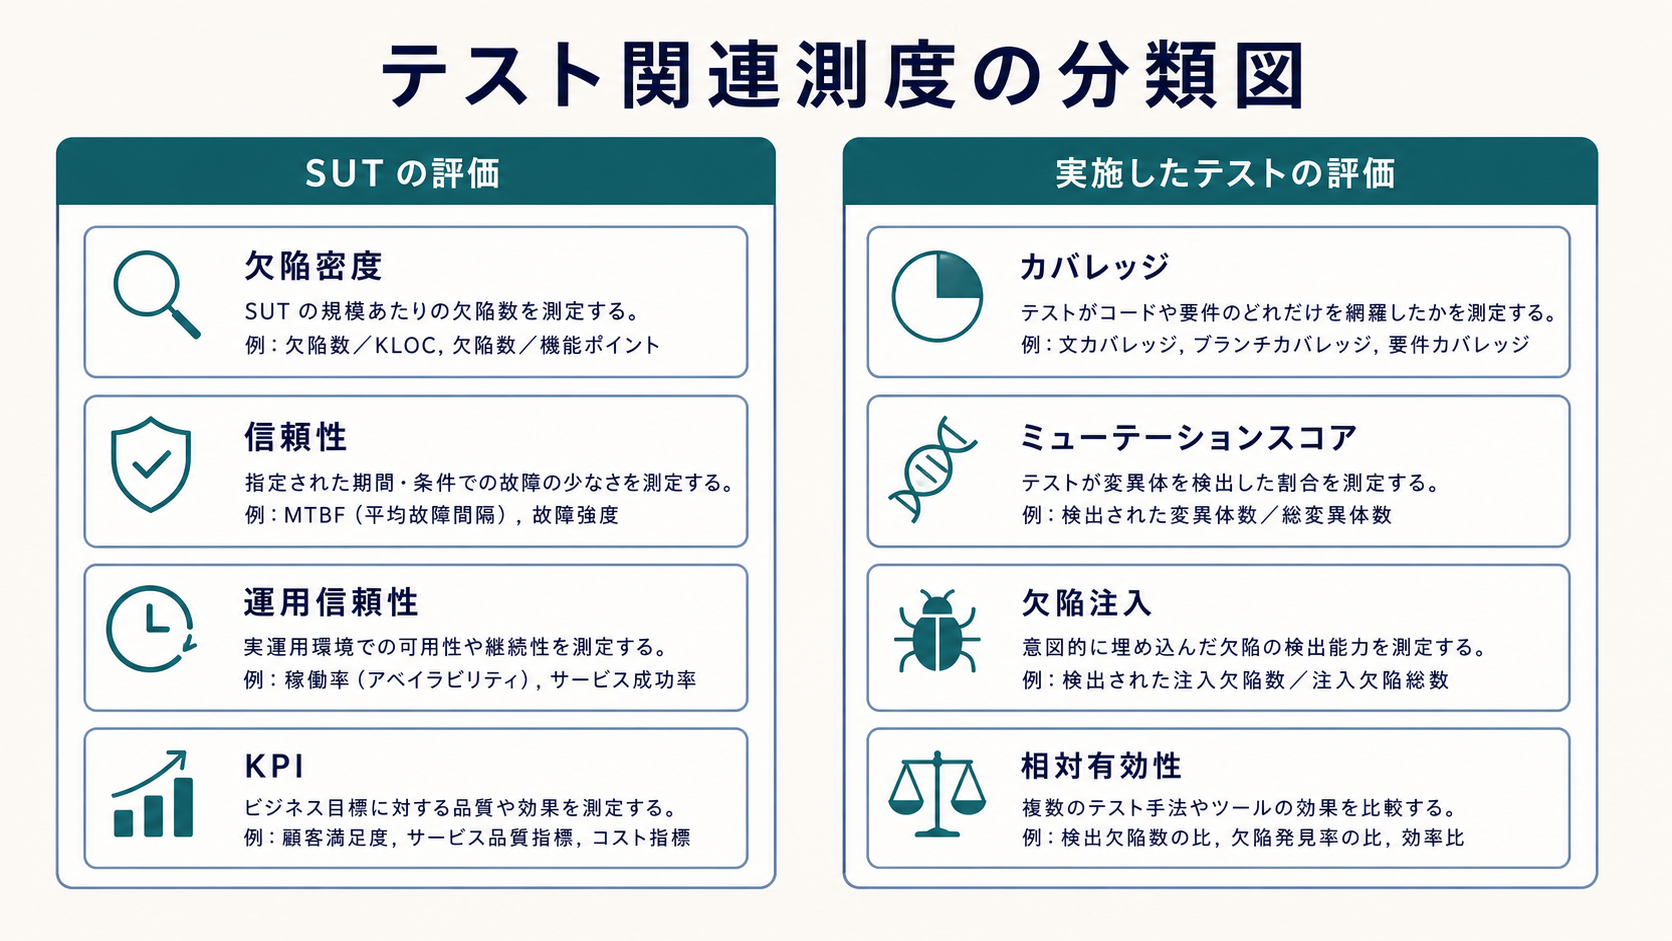
\includegraphics[width=0.96\linewidth]{assets/generated_figures/ch05/fig-ch05-11.png}}{\fbox{\parbox[c][48mm][c]{0.9\linewidth}{\centering 画像生成待ち\\テスト関連測度の分類図}}}
\caption{テスト関連測度の分類図}
\label{fig:ch05-11}
\end{figure}

\subsubsection{SUT の評価}
SUT の評価では、テスト結果から対象システムの状態を判断する。代表的には、欠陥の種類、欠陥密度、信頼性、運用時の障害傾向、主要業績指標が使われる。

\paragraph{テスト計画と設計に役立つ SUT 測定}
テスト計画には、配備頻度、リードタイム、平均回復時間、変更失敗率などの測度が使われることがある。シフトレフトや DevOps では、これらの測度がテストの計画、管理、結果評価と強く結び付く。

\paragraph{欠陥の種類・分類・統計}
欠陥分類は、どの種類の欠陥が多いか、どの品質属性に関係するかを整理する。利用性欠陥、セキュリティ脆弱性、プライバシー攻撃、サイバーリスクなど、対象に応じて分類体系は異なる。過去の発生頻度は、どこにテスト資源を集中するかを決める根拠になる。

\paragraph{欠陥密度}
欠陥密度は、見つかった欠陥数を SUT の規模で割った値である。規模にはコード行数、機能規模、モジュール数などが使われる。欠陥密度だけで品質を完全には表せないが、比較や傾向把握には役立つ。

\paragraph{寿命試験と信頼性評価}
信頼性評価は、テストをいつ止めるか、次のリリースに進めるかを判断するために使われる。クラウドやフォグ環境では、高い信頼性と可用性を維持することが重要であり、テスト活動もその評価に関わる。

\paragraph{信頼性成長モデル}
信頼性成長モデルは、観測された障害と修正の履歴から、信頼性がどのように向上するかを予測する。多くのモデルでは、障害の原因となる欠陥を修正すれば信頼性が増すと仮定する。障害数に注目するモデルと、障害間隔時間に注目するモデルがある。

\subsubsection{実施したテストの評価}
テストそのものの評価では、テストスイートがどれだけ強いか、どの技法が有効かを比較する。カバレッジ、ミューテーション分析、欠陥注入などが用いられる。

\paragraph{欠陥注入}
欠陥注入は、人工的な欠陥を SUT に入れ、テストスイートがそれらをどれだけ検出できるかを調べる。検出率からテスト有効性や残存欠陥数を推定しようとする。ただし、人工欠陥が本物の欠陥を代表しているか、挿入した欠陥を取り残さないかには注意が必要である。

\paragraph{ミューテーションスコア}
ミューテーションスコアは、殺された変異体数を生成した変異体数で割った値である。値が高いほど、テストスイートが小さな変化に敏感であることを示す。ただし、変異体の生成数が多くなるため、実行コストが問題になる。

\paragraph{技法間の比較と相対有効性}
相対有効性は、異なるテスト技法を同じ性質に対して比較する考え方である。最初の障害を見つけるまでのテスト数、欠陥検出率、信頼性改善量などが比較軸になる。

\subsection{テストプロセス}
テスト技法や測度は、定義されたテストプロセスに組み込まれて初めて実務で機能する。テストプロセスは、組織レベル、管理レベル、動的テストレベルの多層構造で考えられる。組織レベルでは方針や戦略を作る。管理レベルでは計画、監視、制御、完了を扱う。動的テストレベルでは設計、実装、環境構築、実行、インシデント報告を扱う。

\begin{figure}[htbp]
\centering
\IfFileExists{assets/generated_figures/ch05/fig-ch05-12.png}{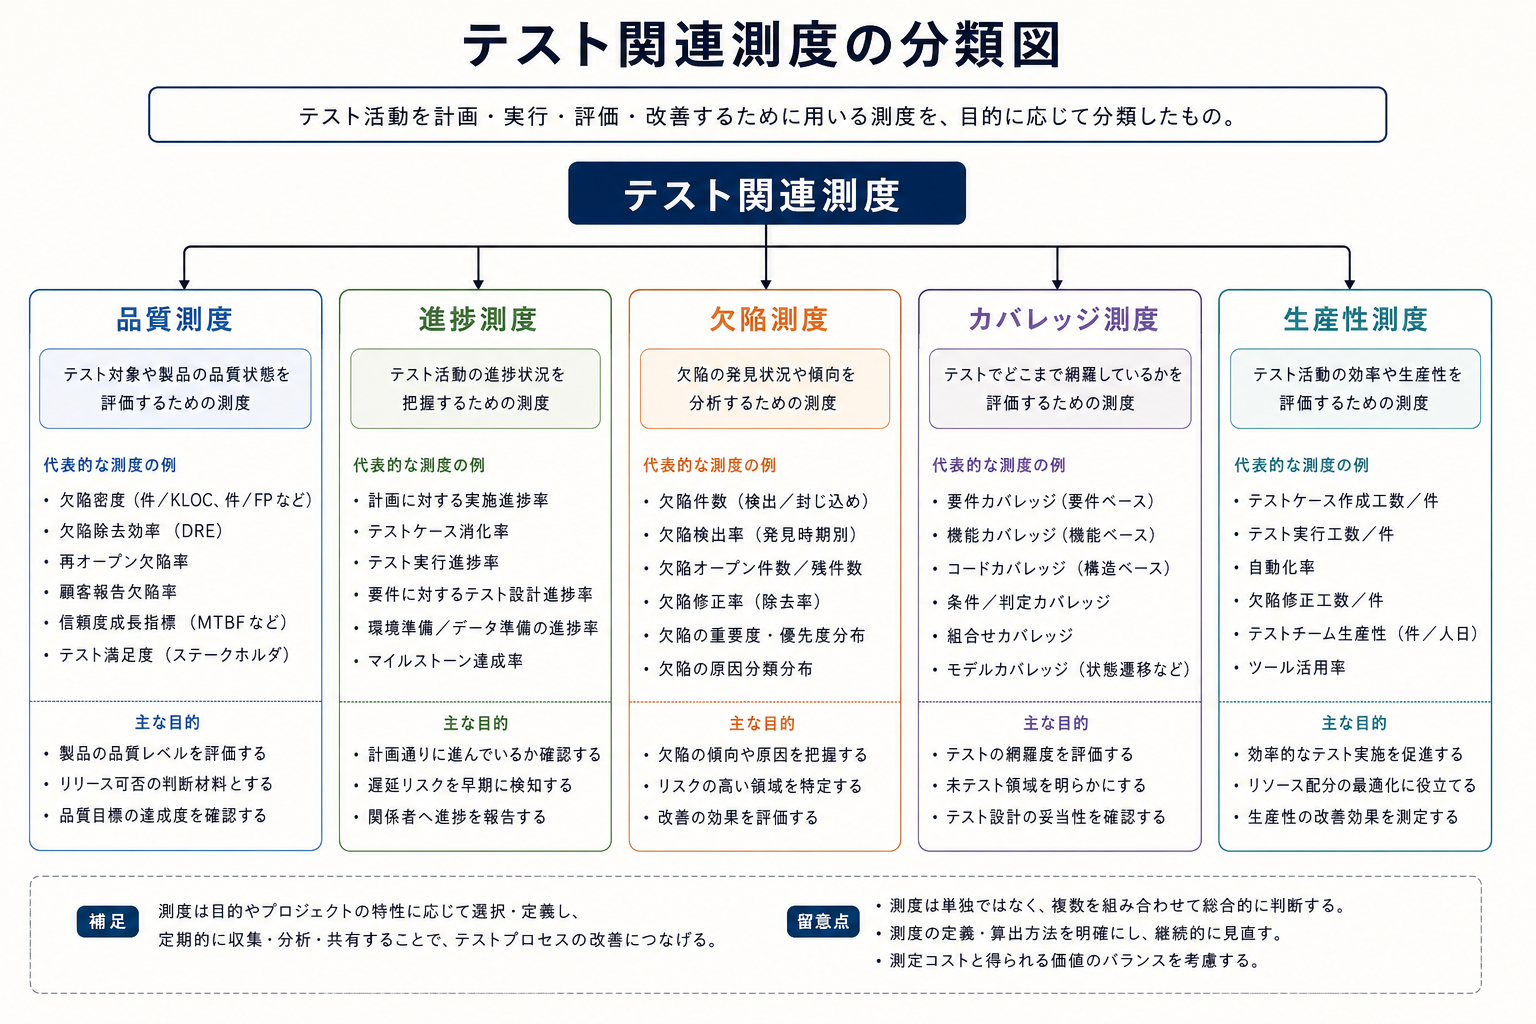
\includegraphics[width=0.96\linewidth]{assets/generated_figures/ch05/fig-ch05-12.png}}{\fbox{\parbox[c][48mm][c]{0.9\linewidth}{\centering 画像生成待ち\\テストプロセスの多層図}}}
\caption{テストプロセスの多層図}
\label{fig:ch05-12}
\end{figure}

\subsubsection{実務上の考慮}
\paragraph{態度とエゴレスプログラミング}
テストで重要なのは、障害発見を個人攻撃と見なさない態度である。欠陥が見つかることは、品質を改善する機会である。管理者は、失敗の発見と修正を歓迎する文化を作る必要がある。アジャイルやシフトレフトでは、テスターと開発者の協調が成功に不可欠である。

\paragraph{テスト指針と組織プロセス}
組織は、テスト方針とテスト戦略を定義する。テスト方針は、テストの目的、目標、全体範囲を示す。テスト戦略は、どのようにテストするかの指針である。リスクベーステストでは、製品リスクをもとにテストの焦点と優先度を決める。

\paragraph{テスト管理と動的テストプロセス}
テスト管理には、計画、監視、制御、完了が含まれる。動的テストプロセスには、テスト設計と実装、テスト環境の準備と保守、テスト実行、インシデント報告が含まれる。これらは、人、ツール、方針、測度を組み合わせてライフサイクルに統合される。

\paragraph{テスト文書化}
テスト文書は、組織テスト文書、テスト管理文書、動的テスト文書に分けられる。組織テスト文書には方針や戦略が含まれる。テスト管理文書にはテスト計画、状況報告、完了報告が含まれる。動的テスト文書にはテスト設計仕様、テストケース仕様、手順仕様、データ要求、環境要求、実行ログ、インシデント報告などが含まれる。

\paragraph{テストチーム}
テストチームの構成は、費用、納期、組織成熟度、アプリケーションの重要度によって変わる。開発者自身がテストする場合も、独立したテスト担当者が行う場合もある。シフトレフトでは、開発者、テスター、顧客が早い段階から協力し、役割の境界が薄くなることがある。

\paragraph{テストプロセス測度}
テストプロセスでは、指定済み、実行済み、合格、不合格のテストケース数、未解決欠陥、解決済み欠陥、欠陥検出率、残存リスク、テスト進捗などを測る。これらは、プロセスリスクの管理、根本原因分析、改善に使われる。

\paragraph{テスト監視と制御}
テスト監視と制御は、テスト活動のデータを収集し、計画どおりに進んでいるかを確認する。必要に応じて、全体計画を修正する。監視は実行と並行して行われ、関係者へ状況報告を提供する。

\paragraph{テスト完了}
テスト完了では、どの程度テストすれば十分か、テスト段階を終えてよいかを判断する。カバレッジ、欠陥密度、信頼性推定は支援情報になるが、それだけでは十分でない。残存障害のリスクと、さらにテストを続ける費用を比較して判断する必要がある。

\paragraph{テスト再利用性}
テスト再利用性は、テストケース、結果、環境、知識を整理し、次のテストや回帰テストで使えるようにすることである。テスト開発が高コストで複雑な場合、再利用性は特に重要である。要求や設計の変更がテストにも反映されるよう、知識リポジトリや追跡が必要である。

\subsubsection{テストサブプロセスと活動}
\paragraph{テスト計画プロセス}
テスト計画では、担当者の調整、テスト目的、完了基準、設備、文書、リスク計画を定義する。組織方針、テスト段階、テスト種類、テスト環境、実行、監視、完了、報告を整える。

\paragraph{テスト設計と実装}
テスト設計と実装では、テストレベルと選んだ技法に基づいてテストケースを作る。ツールを使う場合、ソースコード、仕様、データ構造、テスト基準などを入力し、テストスイートを生成する。場合によっては、期待結果もオラクル機能で生成できる。

\paragraph{テスト環境の構築と保守}
テスト環境は、テストを実行するための設備、ハードウェア、ソフトウェア、ファームウェア、手順を含む。シミュレーション環境、本番に近い環境、監視・ログ機能などを整え、他のソフトウェア工学ツールと互換性を持たせる必要がある。

\paragraph{統制された実験とテスト実行}
テスト実行は、科学的な統制実験の原則を意識すべきである。別の人が結果を再現できるほど、手順、環境、SUT の版、入力、観測結果を明確に記録する。受入テストでは、A/B テストのように利用者の選好を統計的に評価することもある。

\paragraph{テストインシデント報告}
テストインシデント報告は、いつ、誰が、どの構成でテストを行い、どの結果が得られたかを記録する。予期しない結果は問題報告システムに記録され、後のデバッグや変更管理の入力になる。すべての異常が欠陥とは限らないため、分析により原因を特定する必要がある。

\subsubsection{人員配置}
人員配置では、役割、活動、責任、採用、教育を決める。スクラムマスター、テストリード、品質保証担当、テスト分析者、テスト設計者、セキュリティテスト担当、性能テスト担当、環境担当、自動化担当などの役割があり得る。必要な技能が不足すれば、欠陥発見能力、変更対応、納期、保守費用に影響する。

\subsection{開発プロセスと適用領域におけるテスト}
テストは、どの開発プロセスでも基本活動である。ただし、実施の位置づけや用語は、ライフサイクルや適用領域によって変わる。

\subsubsection{ソフトウェア開発プロセス内のテスト}
\paragraph{従来型プロセスにおけるテスト}
逐次型、V 字型、スパイラル、反復型などの従来型プロセスでは、テストが一つの活動として明確に位置づけられることが多い。後半で集中的にテストする場合、利用者ニーズとのずれや評価上の問題が遅く見つかるリスクがある。品質を評価し制御するために、TMMi、SPI、SPICE、CMMI、統一プロセスなどの成熟度モデルや改善枠組みが用いられてきた。

\paragraph{シフトレフトに沿ったテスト}
シフトレフトは、開発の早い段階でテストを採用し、欠陥を早く検出して除去する考え方である。アジャイル、DevOps、TDD はこの動きに含まれる。内部コード品質では、単体・結合テストや構造ベース技法が重要である。業務ニーズでは、システム・受入テスト、利用ベース技法、シナリオベース技法が重要である。知覚品質では、アルファ、ベータ、導入、使いやすさ、セキュリティ、プライバシーが重視される。品質保証では、性能、セキュリティ、プライバシー、適合性、順守が対象になる。

アジャイル開発では、顧客やチームメンバーを含む関係者がテスト活動に関与し、回帰欠陥のリスクや変化する要求への対応が重要になる。TDD では、コードを書く前にテストケースを作り、要求の理解を明確化する。DevOps や継続的インテグレーションでは、回帰テストやスモークテストを継続的に行い、配備前に基本的なテスト可能性を確認する。

\begin{figure}[htbp]
\centering
\IfFileExists{assets/generated_figures/ch05/fig-ch05-13.png}{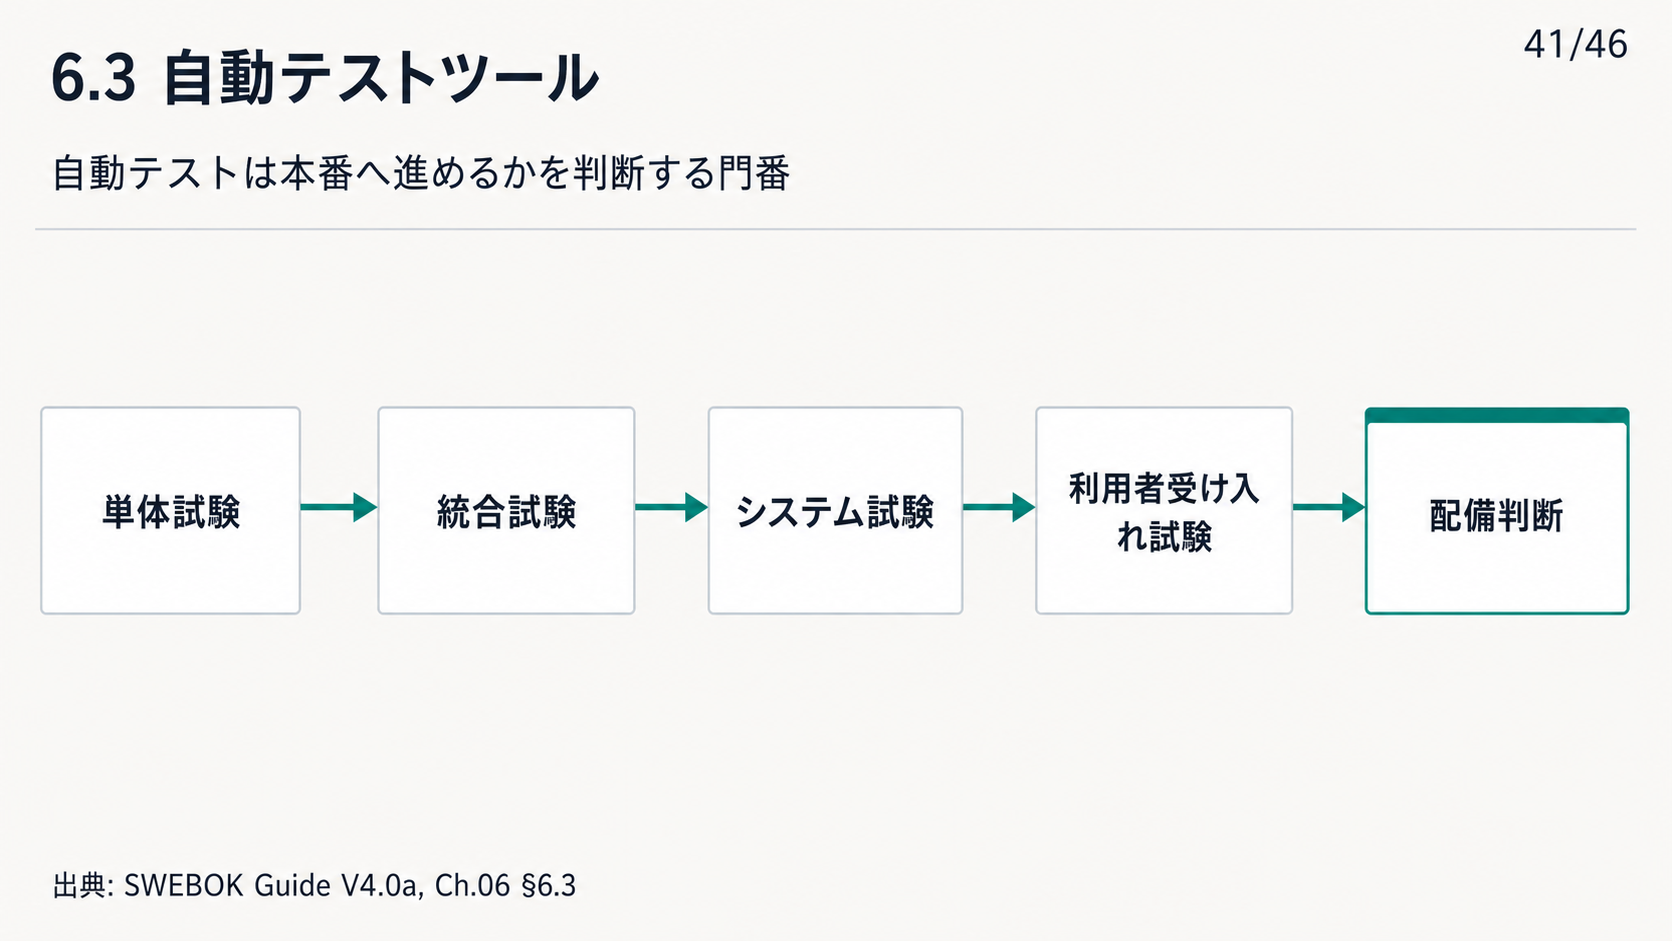
\includegraphics[width=0.96\linewidth]{assets/generated_figures/ch05/fig-ch05-13.png}}{\fbox{\parbox[c][48mm][c]{0.9\linewidth}{\centering 画像生成待ち\\従来型とシフトレフトの比較図}}}
\caption{従来型とシフトレフトの比較図}
\label{fig:ch05-13}
\end{figure}

\subsubsection{適用領域におけるテスト}
適用領域ごとに、重視すべきリスクや標準が異なる。自動車領域では、ソフトウェア、ハードウェア、信号、統合、安全、ストレス、セキュリティが関係する。IoT では、機器管理、異種性、通信、データ、プライバシー、サイバーセキュリティが重要である。法務領域では、高度に機微なデータ、用語、専門家の関与、整合性、順守が重要である。

モバイル領域では、画面解像度、GPS、OS、端末メーカー、ネイティブアプリとウェブアプリの違いを考慮する。航空電子領域では、独立または疎結合の構成要素、市販品、機能・非機能、運用、通信、安全、セキュリティが関係する。医療領域では、安全で信頼できるデータ交換、性能、プライバシー、安全、規制順守が重要である。

組込み領域では、ソフトウェアとハードウェアが密接に結合する。GUI では、画面要素、見た目、配置、誤字、操作感が対象になる。ゲームでは、プレイテスト、機能、セキュリティ、適合性、性能が重要である。リアルタイム領域では、時間制約と決定的振る舞いが重要である。サービス指向、金融、クラウド、AI なども、それぞれ特有の観点を持つ。

\subsection{新興技術のテストと新興技術によるテスト}
新興技術は、テスト対象として新しい課題を生む一方で、テスト活動を支援する手段にもなる。この章では、「新興技術をテストする」と「新興技術を使ってテストする」を分けて理解する。

\begin{figure}[htbp]
\centering
\IfFileExists{assets/generated_figures/ch05/fig-ch05-14.png}{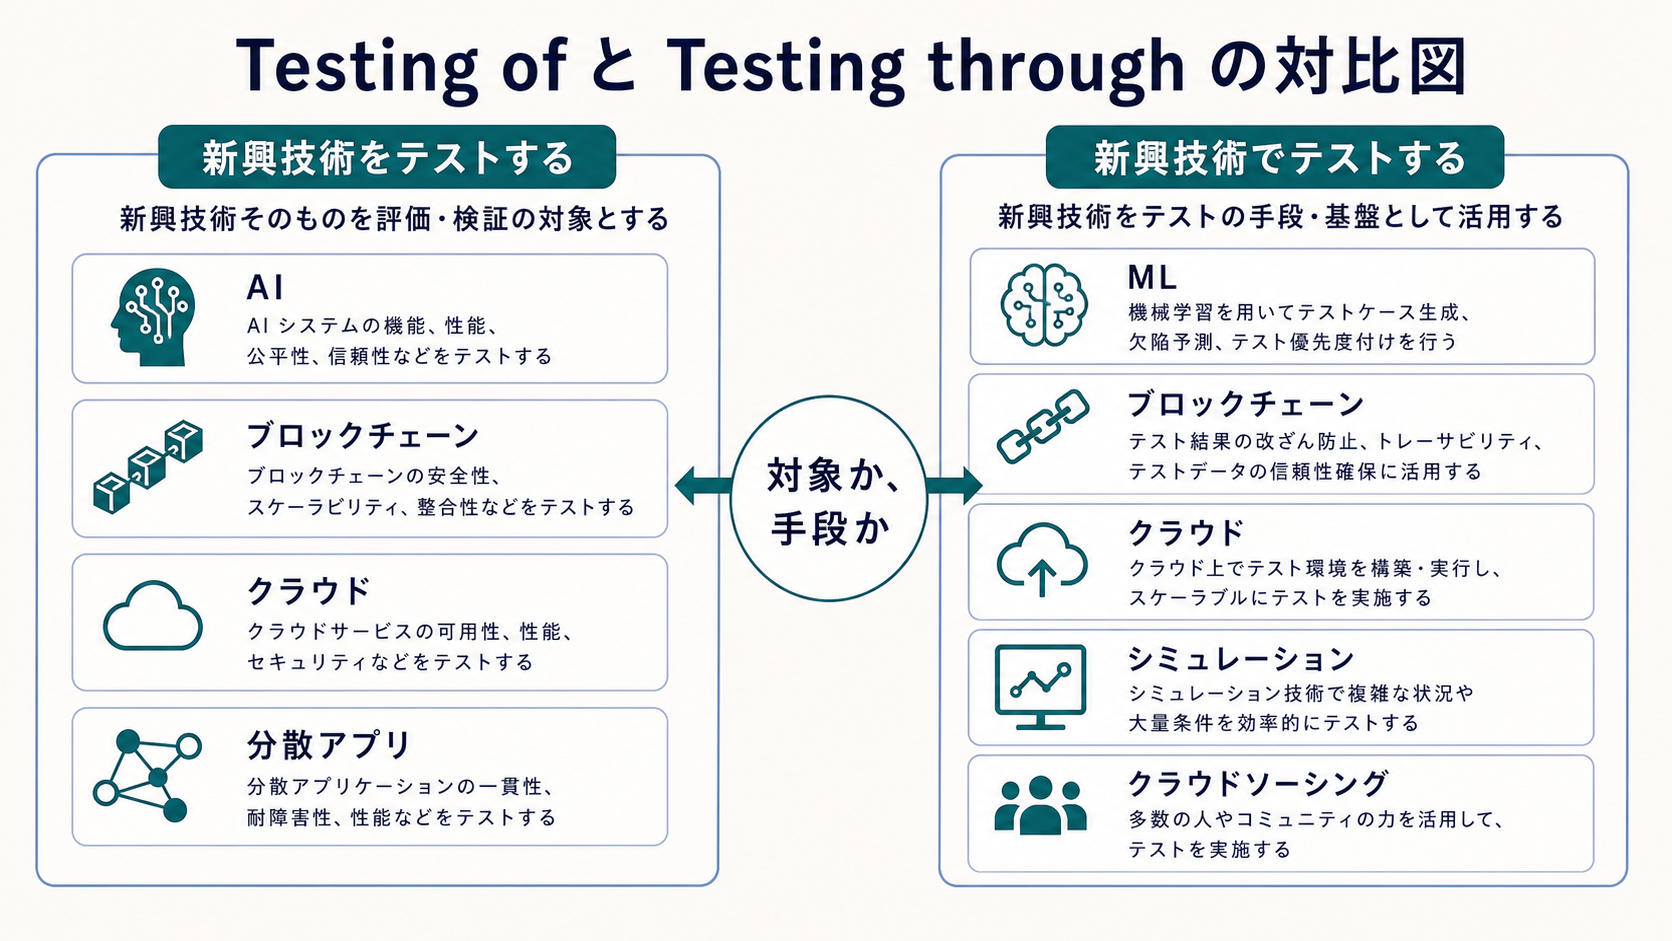
\includegraphics[width=0.96\linewidth]{assets/generated_figures/ch05/fig-ch05-14.png}}{\fbox{\parbox[c][48mm][c]{0.9\linewidth}{\centering 画像生成待ち\\Testing of と Testing through の対比図}}}
\caption{Testing of と Testing through の対比図}
\label{fig:ch05-14}
\end{figure}

\subsubsection{新興技術をテストする}
AI、機械学習、深層学習を使ったシステムでは、非決定性、データ依存性、オラクル問題が大きな課題になる。欠陥は、学習データ、学習プログラム、モデル、フレームワーク、推論環境のどこにでもあり得る。オフラインでは交差検証などでモデルを評価し、配備後はオンラインテストで利用者行動との相互作用を評価する。

ブロックチェーンでは、スマートコントラクトや関連アプリケーションに対して、ストレステスト、侵入テスト、性質テストが使われる。公開型か私有型か、他アプリケーションとの接続、トランザクション性能、セキュリティなどを考慮する。

クラウドでは、クラウド上に配備されたアプリケーションやインフラの機能・非機能品質を確認する。性能、拡張性、弾力性、セキュリティ、互換性、相互運用性が重要である。分散・並行アプリケーションでは、複数 OS、ブラウザ、ハードウェア、利用者、依存関係、継続的配備がテストを複雑にする。

\subsubsection{新興技術を使ってテストする}
機械学習は、テストケース設計、オラクル問題、テスト評価、優先順位付け、ミューテーションテスト自動化、欠陥分類、トリアージに使われる。大量データから傾向を抽出し、保守労力を減らす可能性がある。

ブロックチェーンは、分散した関係者が信頼できる形でテスト活動を調整する手段になり得る。改ざん耐性、監査可能性、分散データ管理、要求順守の自動確認に役立つ可能性がある。クラウドは、大規模シミュレーションや弾力的資源を必要とするテスト環境として利用できる。

シミュレーションは、危険な状況、災害、復旧、特定振る舞いを評価するための重要な手段である。自動車や組込み領域では、実信号を SUT に与えながら現実を模擬するハードウェアインザループテストが使われる。クラウドソーシングテストは、多様な利用者、場所、端末、条件での検出力を得るために使われるが、社内検証の代替ではなく補完である。

\subsection{ソフトウェアテストツール}
テストは、多数の実行、結果の比較、大量の情報管理を伴うため、ツール支援が重要である。ツールは、単純な反復作業を減らし、テスト設計や生成を支援し、効率と有効性を高める。ただし、目的、開発方式、評価対象、実行環境に合うツールを選ぶ必要がある。一つの万能ツールではなく、複数のツールを組み合わせることが多い。

\subsubsection{テストツール支援と選択}
ツール選択では、何を自動化したいか、どの測度を集めたいか、どの環境で実行するか、既存プロセスとどう統合するかを確認する。ツール導入自体にも学習コスト、保守コスト、環境依存、誤判定、オラクルの限界がある。

\subsubsection{ツールの分類}
代表的なツール分類を表に示す。

\par\smallskip\noindent\refstepcounter{table}\label{tab:ch05-03}\textbf{表 \thetable: 第05章 ソフトウェアテスト 表03}\par\smallskip
\begin{longtable}{P{0.27\linewidth}P{0.63\linewidth}}
\toprule
\textbf{分類} & \textbf{主な役割} \\
\midrule
テストハーネス & ドライバやスタブにより、部分的な SUT を制御された環境で実行し、出力を記録する。\\
テスト生成器 & ランダム、経路ベース、モデルベースなどによりテストケースを生成する。\\
キャプチャ・リプレイツール & 以前の入力や画面操作を記録し、再実行する。\\
オラクル・比較・表明検査ツール & 実行結果が成功かどうかの判定を支援する。\\
カバレッジ分析器・計測器 & プログラム中の文、分岐、経路などがどれだけ実行されたかを測る。\\
トレーサ & 実行経路の履歴を記録する。\\
回帰テストツール & 変更後の再実行、影響範囲に基づくテスト選択を支援する。\\
信頼性評価ツール & テスト結果を分析し、信頼性関連測度を可視化する。\\
注入ベースツール & 攻撃注入や欠陥注入により、特定条件での振る舞いを確認する。\\
シミュレーションベースツール & モデルを使ってシナリオを実行し、性質の検証や予測を行う。\\
セキュリティテストツール & 脆弱性、侵入、ファズテストなどを支援する。\\
テスト管理ツール & テスト計画、実行、データ収集、欠陥管理、報告を支援する。\\
クロスブラウザテストツール & 端末やブラウザごとに UI が期待どおり動くかを確認する。\\
負荷テストツール & 性能評価のために負荷を発生させ、関連データを集める。\\
欠陥追跡ツール & 欠陥報告、状態、修正履歴を管理する。\\
モバイルテストツール & 実機やエミュレータで、モバイルアプリの UI や動作を繰り返し確認する。\\
API テストツール & API の機能、性能、信頼性、セキュリティを自動テストする。\\
ウェブアプリケーションテストツール & ウェブベース SUT の機能、性能、利用者向け問題を確認する。\\
\bottomrule
\end{longtable}

\begin{figure}[htbp]
\centering
\IfFileExists{assets/generated_figures/ch05/fig-ch05-15.png}{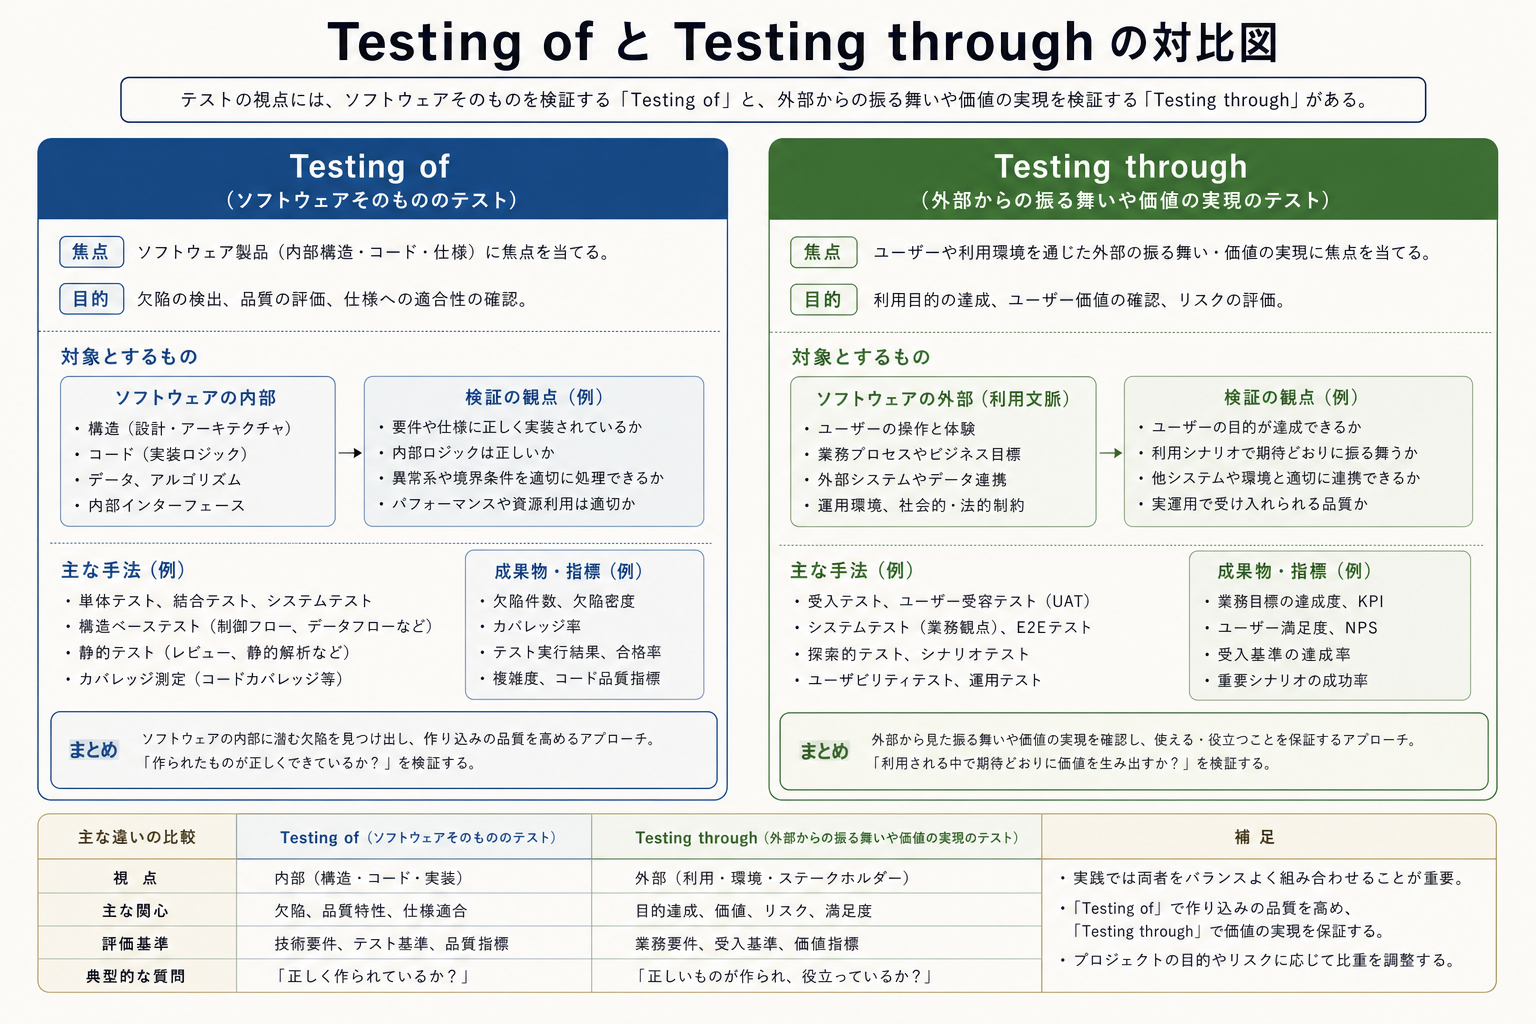
\includegraphics[width=0.96\linewidth]{assets/generated_figures/ch05/fig-ch05-15.png}}{\fbox{\parbox[c][48mm][c]{0.9\linewidth}{\centering 画像生成待ち\\テストツール分類図}}}
\caption{テストツール分類図}
\label{fig:ch05-15}
\end{figure}

\subsection{トピックと参考文献の対応}
この表は、SWEBOK が示す「トピック対参考資料の行列」を、学習用に簡略化したものである。詳しく学ぶときは、各トピックに対応する文献を読む。

\par\smallskip\noindent\refstepcounter{table}\label{tab:ch05-04}\textbf{表 \thetable: 第05章 ソフトウェアテスト 表04}\par\smallskip
\begin{longtable}{P{0.46\linewidth}P{0.46\linewidth}}
\toprule
\textbf{トピック} & \textbf{主な参考資料} \\
\midrule
1. ソフトウェアテストの基礎 & Naik and Tripathy; Sommerville; Laporte and April \\
1.1 欠陥と障害 & Naik and Tripathy; Sommerville; Laporte and April \\
1.2 主要論点 & Naik and Tripathy; ISO/IEC/IEEE 29119; IEEE 1012; ISO/IEC 25010; ISO/IEC/IEEE 32675 \\
1.3 他活動との関係 & Software Quality KA; Software Construction KA; Software Security KA; Professional Practice KA \\
2. テストレベル & Naik and Tripathy; Sommerville \\
2.1 テスト対象 & Naik and Tripathy; Sommerville \\
2.2 テスト目的 & Naik and Tripathy; Sommerville; ISO/IEC/IEEE 29119; ISO/IEC/IEEE 24765; Nielsen \\
3. テスト技法 & Naik and Tripathy; ISO/IEC/IEEE 29119; Utting et al.; Nielsen \\
3.1 仕様ベース技法 & Naik and Tripathy; ISO/IEC/IEEE 29119; Utting et al. \\
3.2 構造ベース技法 & Naik and Tripathy; ISO/IEC/IEEE 29119 \\
3.3 経験ベース技法 & ISO/IEC/IEEE 29119; Riccio et al. \\
3.4 欠陥ベース・ミューテーション & Naik and Tripathy; Papadakis et al.; ISO/IEC/IEEE 24765 \\
3.5 利用ベース技法 & Naik and Tripathy; Sommerville; Nielsen \\
3.6 アプリケーションの性質 & Sommerville; Laporte and April; IEEE 1012 \\
3.7 技法の選択と組合せ & Laporte and April; ISO/IEC/IEEE 32675; ISO/IEC/IEEE 29119 \\
3.8 派生知識に基づく技法 & Sommerville; Laporte and April; Utting et al. \\
4. テスト関連測度 & Sommerville; Laporte and April; ISO/IEC/IEEE 32675; ISO/IEC/IEEE 29119 \\
5. テストプロセス & Sommerville; ISO/IEC/IEEE 29119; SWECOM; ISO/IEC 20246 \\
6. 開発プロセスと適用領域 & Sommerville; Laporte and April; ISO/IEC/IEEE 29119 \\
7. 新興技術のテストと新興技術によるテスト & Riccio et al.; Demi et al.; Bertolino et al.; Achary and Raj; Mao et al. \\
8. ソフトウェアテストツール & Naik and Tripathy; Laporte and April \\
\bottomrule
\end{longtable}

\subsection{参考文献}
\begin{enumerate}[leftmargin=2.2em]
\item S. Naik and P. Tripathy, \textit{Software Testing and Quality Assurance: Theory and Practice}, 1st ed., Wiley, 2008.
\item I. Sommerville, \textit{Software Engineering}, 10th ed., Addison-Wesley, 2016.
\item E. W. Dijkstra, \textit{Notes on Structured Programming}, Technological University, Eindhoven, 1970.
\item ISO/IEC/IEEE 29119, \textit{System and software engineering - Software testing}, 2022.
\item ISO/IEC/IEEE 24765:2017, \textit{Systems and Software Engineering - Vocabulary}, 2nd ed., 2017.
\item M. Papadakis, M. Kintis, J. Zhang, Y. Jia, Y. Le Traon, and M. Harman, ``Mutation Testing Advances: An Analysis and Survey,'' \textit{Advances in Computers}, 112, 2019.
\item M. Utting, B. Legeard, F. Bouquet, E. Fourneret, F. Peureux, and A. Vernotte, ``Recent advances in model-based testing,'' \textit{Advances in Computers}, 101, 2016.
\item IEEE Std 1012-2016, \textit{IEEE Standard for System, Software, and Hardware Verification, and Validation}, 2016.
\item ISO/IEC 25010:2011, \textit{Systems and software Quality Requirements and Evaluation - System and Software Quality Models}, 2011.
\item ISO/IEC/IEEE 32675:2022, \textit{Information technology - DevOps - Building reliable and secure systems including application build, package and deployment}, 2022.
\item Software Engineering Competency Model (SWECOM), v1.0, 2014.
\item ISO/IEC 20246:2017, \textit{Software and systems engineering - Work product reviews}, 2017.
\item V. Riccio, G. Jahangirova, A. Stocco, et al., ``Testing machine learning based systems: A systematic mapping,'' \textit{Empirical Software Engineering}, 25, 2020.
\item C. Y. Laporte and A. April, \textit{Software Quality Assurance}, IEEE Computer Society Press, 1st ed., 2018.
\item S. Demi, R. Colomo-Palacios, and M. Sánchez-Gordón, ``Software Engineering Applications Enabled by Blockchain Technology: A Systematic Mapping Study,'' \textit{Applied Sciences}, 11(7), 2021.
\item K. Mao, L. Capra, M. Harman, and Y. Jia, ``A survey of the use of crowdsourcing in software engineering,'' \textit{Journal of Systems and Software}, 126, 2017.
\item A. Bertolino, G. D. Angelis, M. Gallego, B. García, F. Gortázar, F. Lonetti, and E. Marchetti, ``A systematic review on cloud testing,'' \textit{ACM Computing Surveys}, 52(5), 2019.
\item R. Achary and P. Raj, \textit{Cloud Reliability Engineering: Technologies and Tools}, CRC Press, 2021.
\item J. Nielsen, \textit{Usability Engineering}, 1st ed., Morgan Kaufmann, 1993.
\end{enumerate}

\subsection{章末確認問題}
\begin{enumerate}[leftmargin=2em]
\item 欠陥と障害の違いを説明せよ。なぜテストは欠陥ではなく障害を直接観測することが多いのか。
\item テストケースに入力値以外の情報が必要な理由を説明せよ。
\item テストオラクルとは何か。オラクル問題が起きやすいシステムの例を一つ挙げよ。
\item 単体テスト、結合テスト、システムテスト、受入テストを、対象と目的の観点から比較せよ。
\item 回帰テストがアジャイルや DevOps で重要になる理由を説明せよ。
\item 同値分割と境界値分析の違いを、年齢入力の例で説明せよ。
\item 仕様ベース技法と構造ベース技法はなぜ補完関係にあるのか。
\item 探索的テストが有効になる状況を説明せよ。
\item ミューテーションスコアは何を表すか。値が高いと何が言えるか。
\item テスト完了をカバレッジだけで判断してはいけない理由を説明せよ。
\item シフトレフトの考え方を、従来型プロセスと比較して説明せよ。
\item 「新興技術をテストする」と「新興技術を使ってテストする」の違いを説明せよ。
\end{enumerate}

\begin{pointbox}{解答の方向性}
1 は、原因としての欠陥と観測される結果としての障害を区別する。2 は、状態、環境、手順、期待結果が振る舞いに影響することを述べる。3 は、結果判定の仕組みであり、機械学習や推薦などで難しい。4 は対象の大きさと利用者視点への近さで整理する。5 は変更が頻繁で、既存機能の破壊を早く見つける必要があることを述べる。6 以降は、本文の「選択基準」「十分性」「カバレッジ」「リスク」「費用」「再現性」「目的に応じた技法選択」という語を使って説明できる。
\end{pointbox}

\section{第06章 ソフトウェアエンジニアリング運用}
\begin{pointbox}{この資料の主張}
  ソフトウェアエンジニアリング運用は、完成したソフトウェアを「本番に置く作業」だけではない。運用は、配備、設定、監視、障害対応、変更管理、容量管理、バックアップ、災害復旧、サービス水準、セキュリティ、自動化を含む一連の工学活動である。現代の運用では、開発と運用を分離せず、開発運用連携（DevOps）、インフラストラクチャのコード化（Infrastructure as Code, IaC）、サイト信頼性エンジニアリング（Site Reliability Engineering, SRE）などを使い、ソフトウェアを安全かつ継続的に改善することが重要である。
  \end{pointbox}

\begin{pointbox}{この資料の読み方}
  専門用語は原則として日本語で示し、必要に応じて英語を括弧内に併記する。英語名は、元資料、標準、ツール名を調べる手がかりとして残す。初学者が前提知識なしに読めるように、各節では「何のための概念か」「実務では何を見るべきか」「失敗すると何が起こるか」を重視する。文体は、だである調で統一する。
  \end{pointbox}





\subsection*{全体概要：この章で学ぶこと}
\addcontentsline{toc}{subsection}{全体概要：この章で学ぶこと}

この章は、ソフトウェアを本番環境で安定して動かし続けるための知識領域を扱う。運用は、開発が終わった後に突然始まる作業ではない。新しいソフトウェアを作る意思決定が行われた時点から、運用計画、保守計画、サービス水準、容量、障害時の復旧、セキュリティ、監視、自動化を考え始める必要がある。

\begin{pointbox}{到達目標}
この章を読み終えると、次のことができるようになる。
\begin{itemize}
  \item ソフトウェアエンジニアリング運用の範囲を説明できる。
  \item 運用計画、運用提供、運用制御の三つのプロセス群を区別できる。
  \item 配備とリリース、インシデントと問題、バックアップとフェイルオーバーの違いを説明できる。
  \item 可用性、継続性、サービス水準、容量、リスク管理の関係を説明できる。
  \item DevOps、IaC、SRE、継続的デリバリー、自動テスト、監視とテレメトリが運用にどう関係するかを説明できる。
\end{itemize}
\end{pointbox}

\begin{figure}[htbp]
\centering
\IfFileExists{assets/generated_figures/ch06/fig-ch06-01.png}{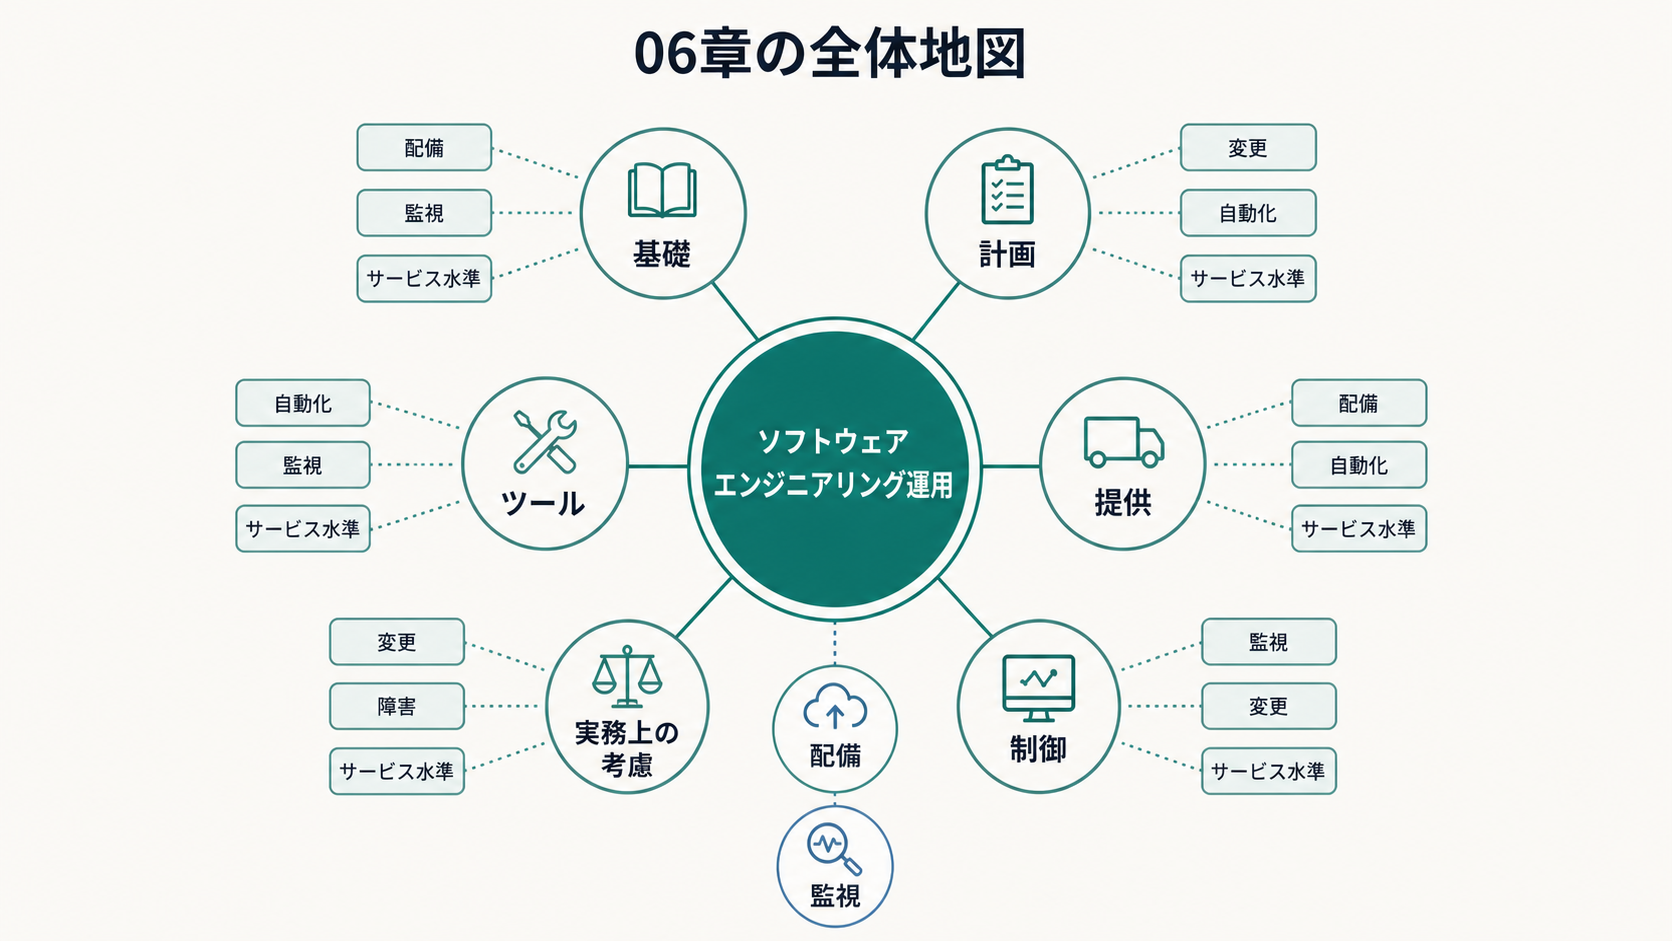
\includegraphics[width=0.96\linewidth]{assets/generated_figures/ch06/fig-ch06-01.png}}{\fbox{\parbox[c][48mm][c]{0.9\linewidth}{\centering 画像生成待ち\\06章の全体地図}}}
\caption{06章の全体地図}
\label{fig:ch06-01}
\end{figure}

\subsection*{最初に必要な用語}
\addcontentsline{toc}{subsection}{最初に必要な用語}

\par\smallskip\noindent\refstepcounter{table}\label{tab:ch06-01}\textbf{表 \thetable: 第06章 ソフトウェアエンジニアリング運用 表01}\par\smallskip
\begin{longtable}{L{35mm}L{115mm}}
\toprule
用語 & 初学者向けの説明 \\
\midrule
ソフトウェアエンジニアリング運用 & ソフトウェアを配備し、動かし、監視し、障害や変更に対応し、利用者へ安定したサービスを提供し続ける活動である。 \\
運用担当技術者 & 運用サービス、配備、監視、障害対応、容量管理、データ保護などを実行または自動化する技術者である。 \\
開発運用連携（DevOps） & 開発、保守、運用の間の壁を低くし、共通のプロセスとツールで素早く安全にソフトウェアを改善する考え方である。 \\
インフラストラクチャのコード化（IaC） & サーバ、ネットワーク、設定、環境構築などを手作業ではなくコードとして表し、再現可能に管理する方法である。 \\
プラットフォーム工学 & 開発者が自分で環境構築、配備、監視などを使えるように、内部向けの共通基盤を作る活動である。 \\
サイト信頼性エンジニアリング（SRE） & 可用性、性能、遅延、容量、緊急対応などを、ソフトウェア工学の方法で改善する運用の考え方である。 \\
サービス水準合意（SLA） & サービスの可用性、応答時間、復旧時間などについて、提供者と利用者の間で合意した水準である。 \\
インシデント & サービスの正常な運用を妨げる出来事である。障害、性能劣化、誤設定、セキュリティ事象などが含まれる。 \\
問題 & 一つまたは複数のインシデントの背後にある原因、または原因候補である。 \\
テレメトリ & ソフトウェアやインフラから収集する運用データである。ログ、実行トレース、CPU使用量、メモリ使用量、利用者操作などが含まれる。 \\
\bottomrule
\end{longtable}

\subsection*{導入：運用が重要な理由}
\addcontentsline{toc}{subsection}{導入：運用が重要な理由}

ソフトウェアエンジニアリング運用とは、ソフトウェアまたはシステムの完全性と安定性を保ちながら、配備し、運用し、支援するために必要な活動と作業である。ここでいう運用は、対象環境へのソフトウェアの配備と設定、利用中の監視と管理、欠陥対応、環境変更への対応、新しい利用者要求への対応を含む。

従来、運用部門や計算センターは、開発部門から分離された組織として扱われることが多かった。この分離は、引き継ぎの遅れ、手作業による設定ミス、責任境界の曖昧化、リリースの遅延を生みやすい。現在は、開発、保守、運用を近づけ、DevOps、IaC、プラットフォーム工学、SREなどを使って、変更を早く、かつ安全に本番へ届ける考え方が広がっている。

この章で重要な視点は二つである。第一に、運用は「最後に引き受ける部門作業」ではなく、開発初期から設計されるサービスである。第二に、現代の運用では、環境、設定、配備、監視、試験、復旧をできるだけコードと自動化で表すことで、再現性、標準化、セキュリティ、変更管理、拡張性を高める。

\begin{pointbox}{重要}
運用の品質は、利用者が直接体験するソフトウェアの品質である。コードが正しくても、配備が失敗し、監視できず、復旧できず、容量が足りなければ、利用者から見たサービスは失敗である。
\end{pointbox}

\subsection{ソフトウェアエンジニアリング運用の基礎}

\subsubsection{ソフトウェアエンジニアリング運用の定義}

ソフトウェアエンジニアリング運用とは、ソフトウェア製品、情報技術インフラ、システムソフトウェア、アプリケーションソフトウェアが、開発中、保守中、実運用中に適切に動作するように使われる知識、技能、プロセス、ツールの総体である。

運用担当技術者は、単にサーバを見張る人ではない。コンテナや仮想サーバの準備、配備、設定、支援を行う。必要な環境をオンデマンドで提供し、継続的インテグレーション、試験、配備、監視をサービスとして提供する。障害を診断し、問題と解決策を記録し、優先順位を付け、影響を評価する。さらに、セキュリティ、データ保護、フェイルオーバー、容量、ストレージ、データベース性能、技術仕様書の整備にも関わる。

\par\smallskip\noindent\refstepcounter{table}\label{tab:ch06-02}\textbf{表 \thetable: 第06章 ソフトウェアエンジニアリング運用 表02}\par\smallskip
\begin{longtable}{L{45mm}L{105mm}}
\toprule
役割 & 主な責任 \\
\midrule
運用担当技術者 & 運用サービスを設計し、配備、監視、容量管理、障害対応、セキュリティ、復旧を実行または自動化する。 \\
ソフトウェア技術者 & 運用担当技術者が提供する運用サービスを使い、自分のソフトウェアを配備、監視、改善する。 \\
プラットフォーム技術者 & 開発者が自律的に使える共通基盤、セルフサービス環境、配備基盤、監視基盤を作る。 \\
SRE技術者 & 可用性、性能、遅延、容量、緊急対応、変更管理を、測定と自動化に基づいて改善する。 \\
\bottomrule
\end{longtable}

\subsubsection{ソフトウェアエンジニアリング運用プロセス}

運用プロセスは、既存のソフトウェアシステムまたは製品を配備、設定、運用、支援し、その完全性を保つための活動である。国際標準では、運用の準備、運用の実行、運用結果の管理、利用者支援が重要な活動として扱われる。

SWEBOK 06章では、運用活動を学習しやすくするため、次の三つのプロセス群として整理できる。

\par\smallskip\noindent\refstepcounter{table}\label{tab:ch06-03}\textbf{表 \thetable: 第06章 ソフトウェアエンジニアリング運用 表03}\par\smallskip
\begin{longtable}{L{35mm}L{115mm}}
\toprule
プロセス群 & 含まれる活動 \\
\midrule
運用計画 & 運用計画、供給者管理、開発環境と運用環境、可用性、継続性、サービス水準、容量、バックアップ、災害復旧、フェイルオーバー、安全性とセキュリティを扱う。 \\
運用提供 & 運用テスト、検証、受け入れ、配備、リリース、ロールバック、データ移行、問題解決を扱う。 \\
運用制御 & インシデント管理、変更管理、監視、測定、追跡、レビュー、運用支援、サービス報告を扱う。 \\
\bottomrule
\end{longtable}

\begin{figure}[htbp]
\centering
\IfFileExists{assets/generated_figures/ch06/fig-ch06-02.png}{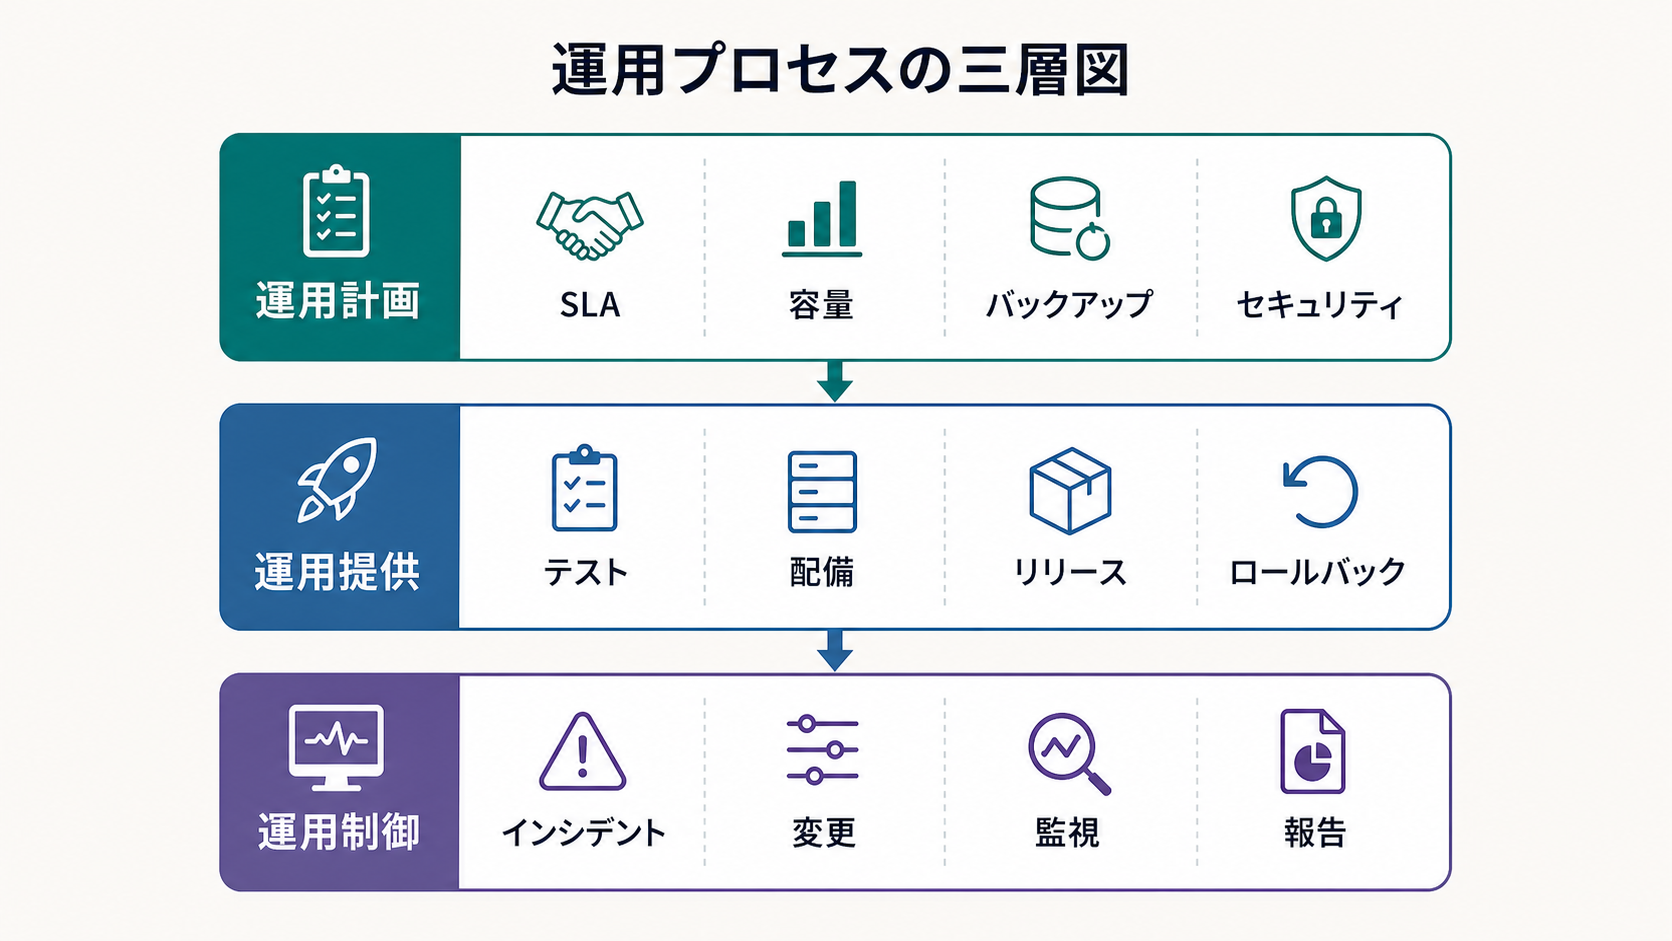
\includegraphics[width=0.96\linewidth]{assets/generated_figures/ch06/fig-ch06-02.png}}{\fbox{\parbox[c][48mm][c]{0.9\linewidth}{\centering 画像生成待ち\\運用プロセスの三層図}}}
\caption{運用プロセスの三層図}
\label{fig:ch06-02}
\end{figure}

\subsubsection{ソフトウェア導入}

ソフトウェア導入とは、ソフトウェアまたは更新版を利用者に使える状態にするため、対象環境に配置し、設定し、確認する作業である。導入では、旧版の削除、対象環境に合わせた設定、必要なディレクトリ、登録情報、環境変数の作成などが行われる。多くの場合、これらはスクリプトで実行される。

組込みシステムでは、電子的な配布だけでなく、物理媒体を使うこともある。いずれの場合でも、導入後には検証が必要である。導入が成功したか、必要なファイルが配置されたか、設定が正しいか、最低限の動作確認ができるかを確認する。

\subsubsection{スクリプト化と自動化}

スクリプト化とは、繰り返し行う作業を簡易なプログラムとして記述することである。自動化とは、人が手作業で行っていた処理を、ツールやスクリプトで再現可能に実行することである。運用では、環境構築、設定変更、配備、監視、通知、ログ収集、バックアップ、復旧試験など、多くの活動が自動化の対象になる。

自動化には三つの効果がある。第一に、遅延を減らせる。第二に、手作業のばらつきや設定ミスを減らせる。第三に、障害時の反応を早め、停止時間を短くできる。さらに、自動化された手順は標準化され、運用サービスとして開発者へ提供しやすくなる。

\begin{pointbox}{実務で見るべきこと}
自動化は「便利だから行う」のではない。変更を安全に早く届けるため、同じ環境を何度でも作れるようにするため、障害時に人間の記憶へ依存しないために行うのである。
\end{pointbox}

\subsubsection{効果的なテストとトラブルシューティング}

運用はシステムの安定性に責任を持つ。そのため、ソフトウェアは本番配備前に十分に試験されなければならない。手作業の試験は時間がかかり、誤りや漏れが発生しやすく、大規模化しにくい。したがって、単体試験、統合試験、システム試験、受け入れ試験、回帰試験を可能な限り自動化することが重要である。

本番でエラーが見つかった場合、運用担当技術者とソフトウェア技術者は、診断を実行し、問題と解決策を記録し、優先順位を付け、影響を評価する。報告された問題が実際に再現するかを確認することも重要である。大規模ソフトウェアに対して全面的な再試験を毎回行うことは高価であるため、回帰試験や試験網羅の戦略が必要になる。

本番環境での試験は難しい。停止できない重要システムでは、カナリア試験や暗黙リリースなどを使い、一部の利用者や裏側の経路だけで新機能を観察する方法が使われる。

\subsubsection{性能、信頼性、負荷分散}

性能、信頼性、負荷分散は、開発初期から計画されるべきである。性能とは、応答時間や処理量が期待水準を満たすことである。信頼性とは、故障しにくく、期待どおりに動き続けることである。負荷分散とは、複数のサーバや資源に処理を振り分け、過負荷や単一点障害を避けることである。

現代の運用では、需要に応じてインフラを動的に増減させることが重視される。DevOpsの考え方を使うと、運用担当技術者は開発段階から必要なインフラサービスを用意し、ソフトウェア技術者は開発中からそれを使って試験できる。

\subsection{ソフトウェアエンジニアリング運用計画}

運用計画は、ソフトウェアを運用し続けるための準備を体系化する活動である。運用は多くの場合、開発期間より長く続く。したがって、運用計画では、短期の配備だけでなく、長期の保守、支援、容量、サービス水準、コスト、人員、供給者、セキュリティを考える必要がある。

運用担当技術者は、作業手順やツールを、目的に合う形で文書化する。証拠として残すべきものには、方針と計画、サービス文書、手順、プロセス、プロセス制御記録がある。

\subsubsection{運用計画と供給者管理}

\paragraph{運用計画}

運用計画は、プロジェクト要求、開発者や保守担当者のニーズを、運用サービスへ翻訳する活動である。開発は数か月から数年で終わることが多いが、運用は何年も続く。そのため、資源見積もり、人員計画、教育、予算、容量、支援体制を早くから考えることが重要である。

新しいソフトウェアを開発すると決めた時点で、運用と保守の要求を考慮すべきである。概念文書、運用保守計画、運用構想（Concept of Operations, CONOPS）を作り、利用者が変更要求や問題報告をどのように出すか、誰が受け付けるか、どのように優先順位を付けるか、どのようにリリースへ反映するかを明らかにする。

\par\smallskip\noindent\refstepcounter{table}\label{tab:ch06-04}\textbf{表 \thetable: 第06章 ソフトウェアエンジニアリング運用 表04}\par\smallskip
\begin{longtable}{L{45mm}L{105mm}}
\toprule
運用計画で扱う項目 & 説明 \\
\midrule
役割と責任 & 新しいサービスまたは変更されたサービスを、誰が実装、運用、保守するかを決める。 \\
顧客と供給者の活動 & 顧客側と供給者側が行う作業、契約、合意を明確にする。 \\
要員と教育 & 必要な人員、技能、訓練、技術支援を計画する。 \\
プロセスとツール & 使う手順、測定、方法、ツールを定義する。 \\
容量と財務 & 将来の利用量、予算、時程、費用を見積もる。 \\
サービス受け入れ基準 & 運用開始できると判断する条件を決める。 \\
期待成果 & 運用した結果として何を測定し、どの水準を満たすかを数値で表す。 \\
\bottomrule
\end{longtable}

個々の問題報告や変更要求のレベルでは、対象となるリリース日、次版の内容、潜在的な衝突、リスク、ロールバック計画、データ移行計画、関係者への通知を扱う。

\begin{figure}[htbp]
\centering
\IfFileExists{assets/generated_figures/ch06/fig-ch06-03.png}{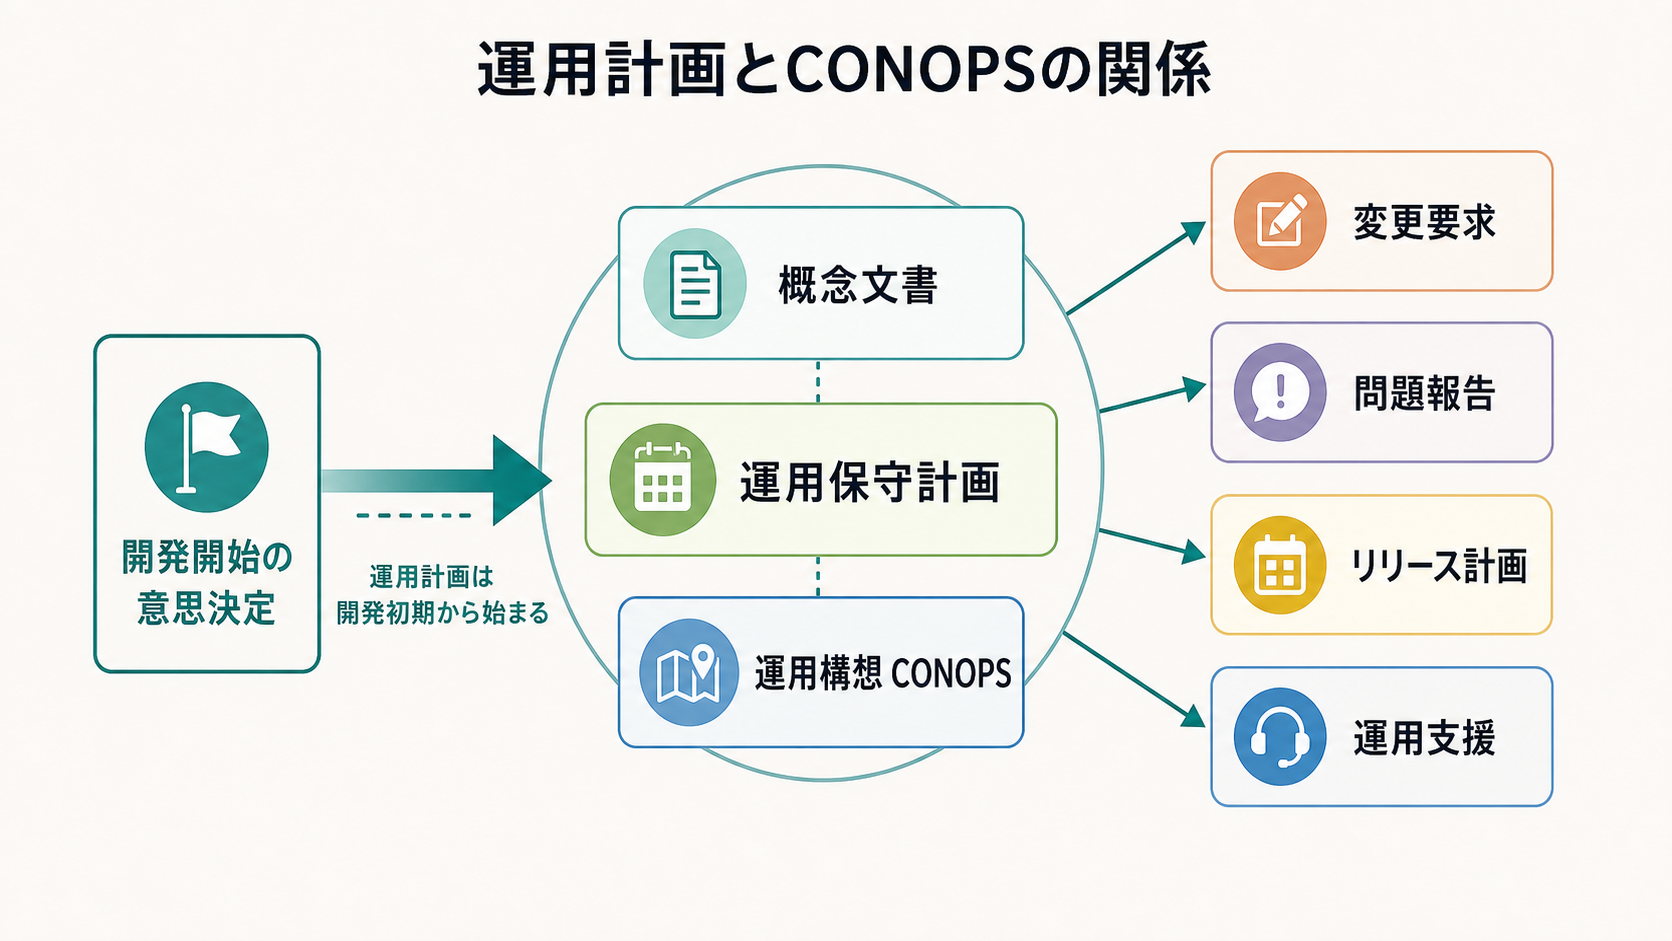
\includegraphics[width=0.96\linewidth]{assets/generated_figures/ch06/fig-ch06-03.png}}{\fbox{\parbox[c][48mm][c]{0.9\linewidth}{\centering 画像生成待ち\\運用計画とCONOPSの関係}}}
\caption{運用計画とCONOPSの関係}
\label{fig:ch06-03}
\end{figure}

\paragraph{供給者管理}

供給者管理とは、外部供給者の製品やサービスを、品質の高い運用サービスに結びつくように管理する活動である。ここでいう供給者には、外部委託先、クラウドサービス、インフラ提供者、プラットフォーム提供者、監視ツール提供者などが含まれる。

運用担当技術者は、供給者との関係を、製品やサービスの性質に合わせて決める。たとえば、サービスとしてのインフラ（IaaS）やサービスとしてのプラットフォーム（PaaS）を使う場合、契約、責任分界点、可用性、障害通知、データ保護、監査、終了時の移行を確認しなければならない。

\subsubsection{開発環境と運用環境}

ソフトウェアプロセスでは、開発環境、試験環境または品質保証環境、事前本番環境、本番環境が使われる。品質を作り込み、本番リリースのリスクを下げるには、これらの環境が一貫しており、本番環境と同期している必要がある。

\par\smallskip\noindent\refstepcounter{table}\label{tab:ch06-05}\textbf{表 \thetable: 第06章 ソフトウェアエンジニアリング運用 表05}\par\smallskip
\begin{longtable}{L{35mm}L{115mm}}
\toprule
環境 & 目的 \\
\midrule
開発環境 & 開発者がコードを書き、単体試験や小規模な確認を行う環境である。 \\
試験・品質保証環境 & 統合試験、品質保証、回帰試験、自動試験を実行する環境である。 \\
事前本番環境 & 本番に近い条件で、配備手順、性能、運用手順を確認する環境である。 \\
本番環境 & 実際の利用者にサービスを提供する環境である。 \\
\bottomrule
\end{longtable}

DevOpsでは、これらの環境を単一のコードリポジトリから自動的に作成することが推奨される。すべての環境が同じコード源から作られれば、環境差分による不具合を減らせる。これがインフラストラクチャのコード化につながる。

\begin{figure}[htbp]
\centering
\IfFileExists{assets/generated_figures/ch06/fig-ch06-04.png}{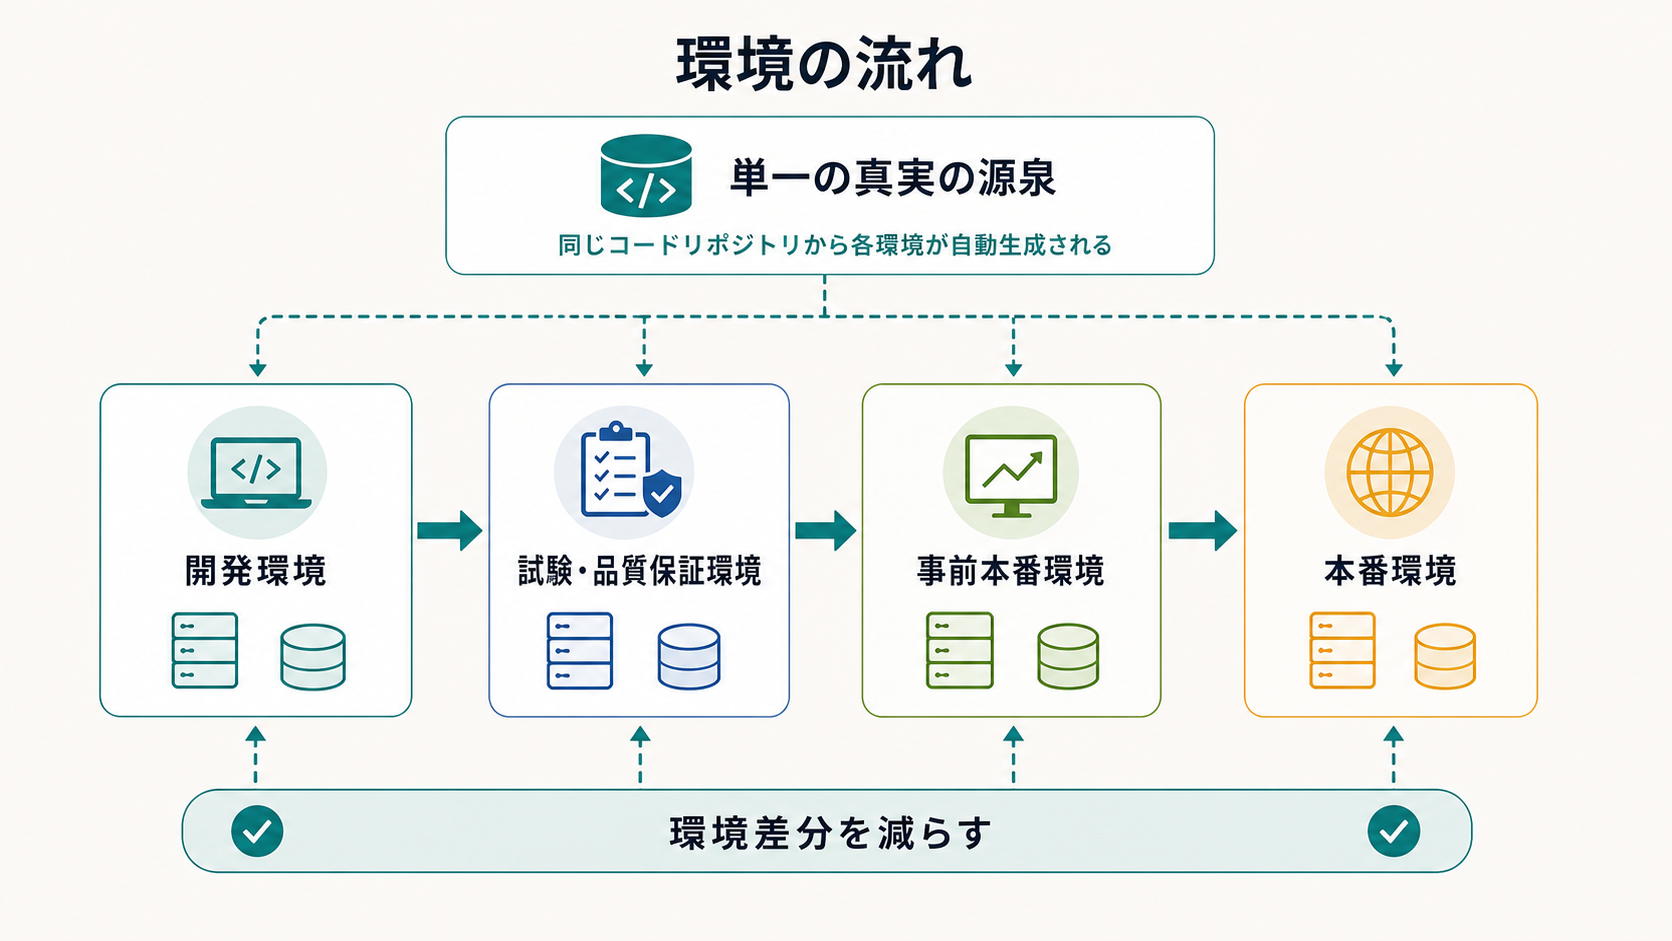
\includegraphics[width=0.96\linewidth]{assets/generated_figures/ch06/fig-ch06-04.png}}{\fbox{\parbox[c][48mm][c]{0.9\linewidth}{\centering 画像生成待ち\\環境の流れ}}}
\caption{環境の流れ}
\label{fig:ch06-04}
\end{figure}

\subsubsection{ソフトウェア可用性、継続性、サービス水準}

可用性とは、必要なときにサービスが利用可能である度合いである。継続性とは、大きな障害や災害が発生してもサービスを維持または復旧できる能力である。サービス水準とは、可用性、性能、応答時間、復旧時間などについて合意された水準である。

運用担当技術者は、プロジェクト初期に非機能要求として定義された可用性と継続性を満たすため、適切なインフラを計画、設計、実装、試験する。可用性は測定され、記録され、予定外の停止は調査される。サービス報告では、合意されたサービス水準に対して、実際の運用がどうだったかを示す。

SLAは、運用サービスの義務を明確にするために有効である。SLAがなければ、利用者は「常に速く、絶対に止まらない」ことを期待し、提供者は「通常は動いている」と考えるかもしれない。合意された水準がなければ、運用の成否を客観的に判断しにくい。

\subsubsection{ソフトウェア容量管理}

容量管理とは、現在と将来の需要に対して、十分な処理能力、記憶容量、ネットワーク、データベース性能などを確保する活動である。利用者数、トランザクション数、データ量、業務量の変化を予測し、それを具体的な要求に変換して文書化する。

容量管理は、性能と容量の問題の中心となる。新規サービスや変更サービスを設計するとき、想定負荷を見積もり、必要な資源をモデル化する。容量計画には、現在の性能、将来要求、費用を伴う選択肢、SLA達成のための推奨策を含める。

\begin{pointbox}{例}
動画配信サービスで、通常時は一日10万人が利用するが、イベント配信時には同時接続が10倍になると予測される場合、容量管理ではピーク時のサーバ数、ネットワーク帯域、キャッシュ戦略、負荷分散、監視しきい値を計画する必要がある。
\end{pointbox}

\subsubsection{バックアップ、災害復旧、フェイルオーバー}

バックアップとは、データ、文書、ソフトウェアを復旧できるように複製して保管することである。災害復旧とは、大規模障害や災害後にサービスを復元する活動である。フェイルオーバーとは、主系が故障したときに、予備系へ切り替えてサービスを継続する仕組みである。

復旧を成功させるには、どのバックアップ方式を使うか、どの頻度で復元点を作るか、どこに保管するか、どれくらい保持するかを決める必要がある。完全バックアップは全体を保存する方式であり、増分バックアップは前回からの差分を保存する方式である。

重要なのは、バックアップを取ることではなく、復旧できることである。災害復旧とフェイルオーバーは、計画され、定期的にリハーサルされる必要がある。ソフトウェア側にも障害処理の論理が必要であり、これは開発時に計画されなければならない。

\begin{figure}[htbp]
\centering
\IfFileExists{assets/generated_figures/ch06/fig-ch06-05.png}{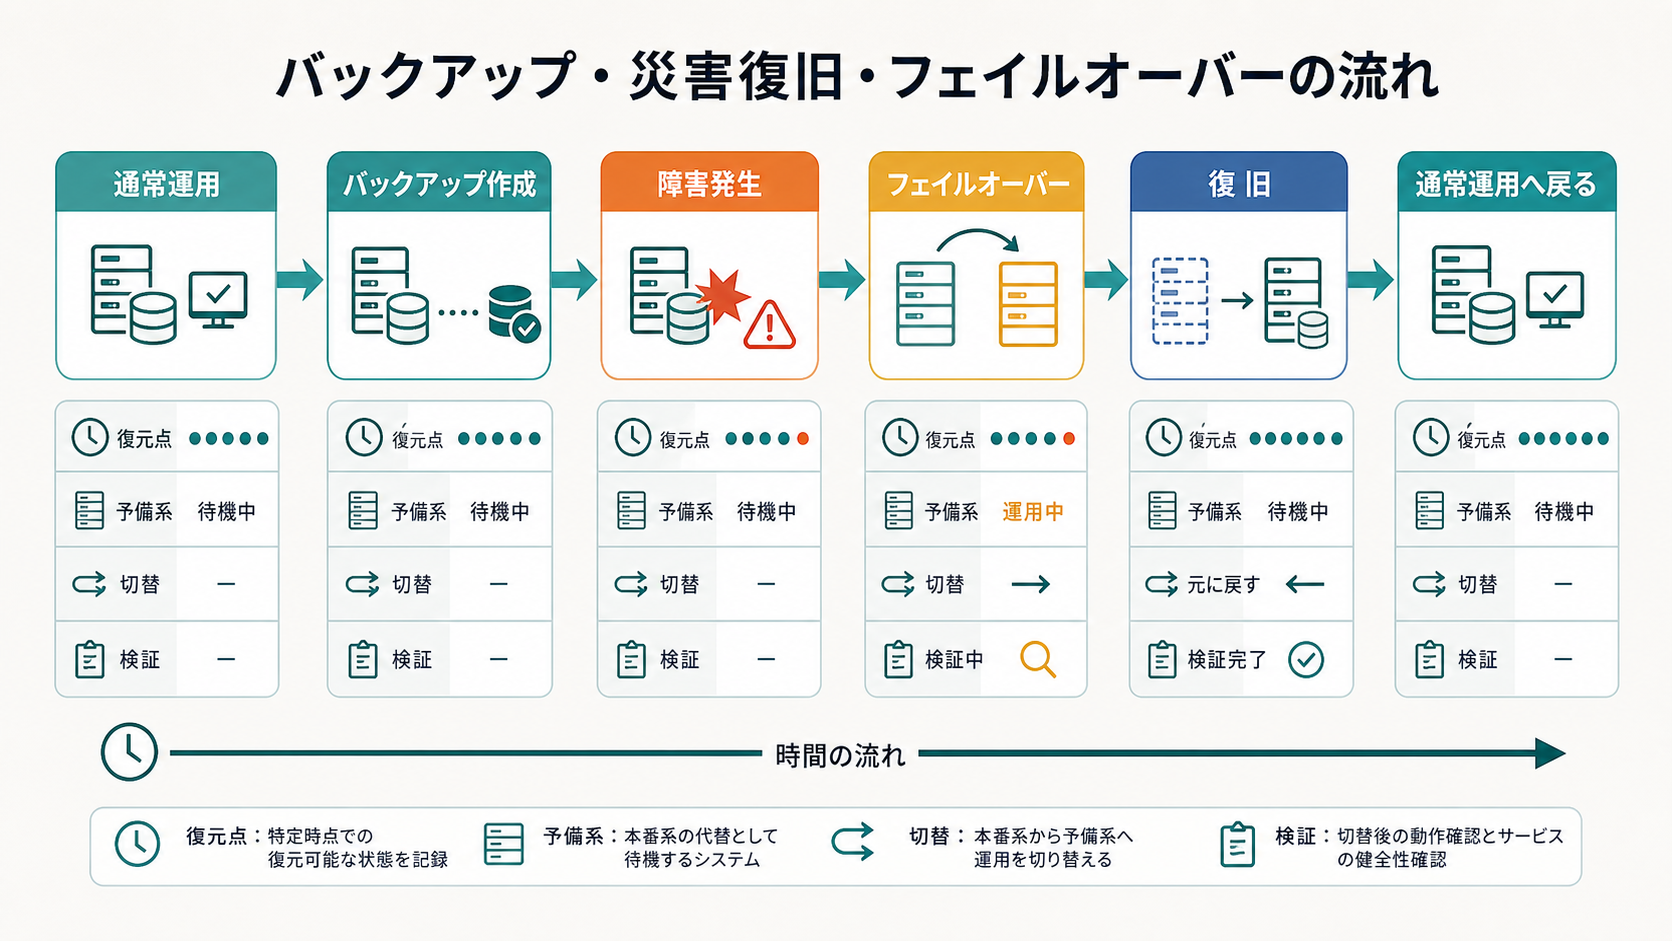
\includegraphics[width=0.96\linewidth]{assets/generated_figures/ch06/fig-ch06-05.png}}{\fbox{\parbox[c][48mm][c]{0.9\linewidth}{\centering 画像生成待ち\\バックアップ・災害復旧・フェイルオーバーの流れ}}}
\caption{バックアップ・災害復旧・フェイルオーバーの流れ}
\label{fig:ch06-05}
\end{figure}

\subsubsection{ソフトウェアとデータの安全性、セキュリティ、完全性、保護、統制}

運用では、情報セキュリティをすべてのサービス活動の中で管理する必要がある。これは、情報の安全性と可用性に関するリスク評価を行い、統制を実施することである。

運用で考えるべき統制には、経営層による情報セキュリティ方針の定義、役割と責任の割当、方針の有効性を監視する責任者、セキュリティ教育、全職員への方針周知、リスク評価と統制実装に関する専門的支援、変更が統制を壊さないことの確認、セキュリティインシデントの報告と対応が含まれる。

DevOpsの発展に伴い、開発運用セキュリティ連携（DevSecOps）が重要になっている。DevSecOpsでは、セキュリティを後工程で追加するのではなく、開発と運用の最初から組み込み、セキュリティ問題の検出と修正をできるだけ早く自動化する。

\begin{figure}[htbp]
\centering
\IfFileExists{assets/generated_figures/ch06/fig-ch06-06.png}{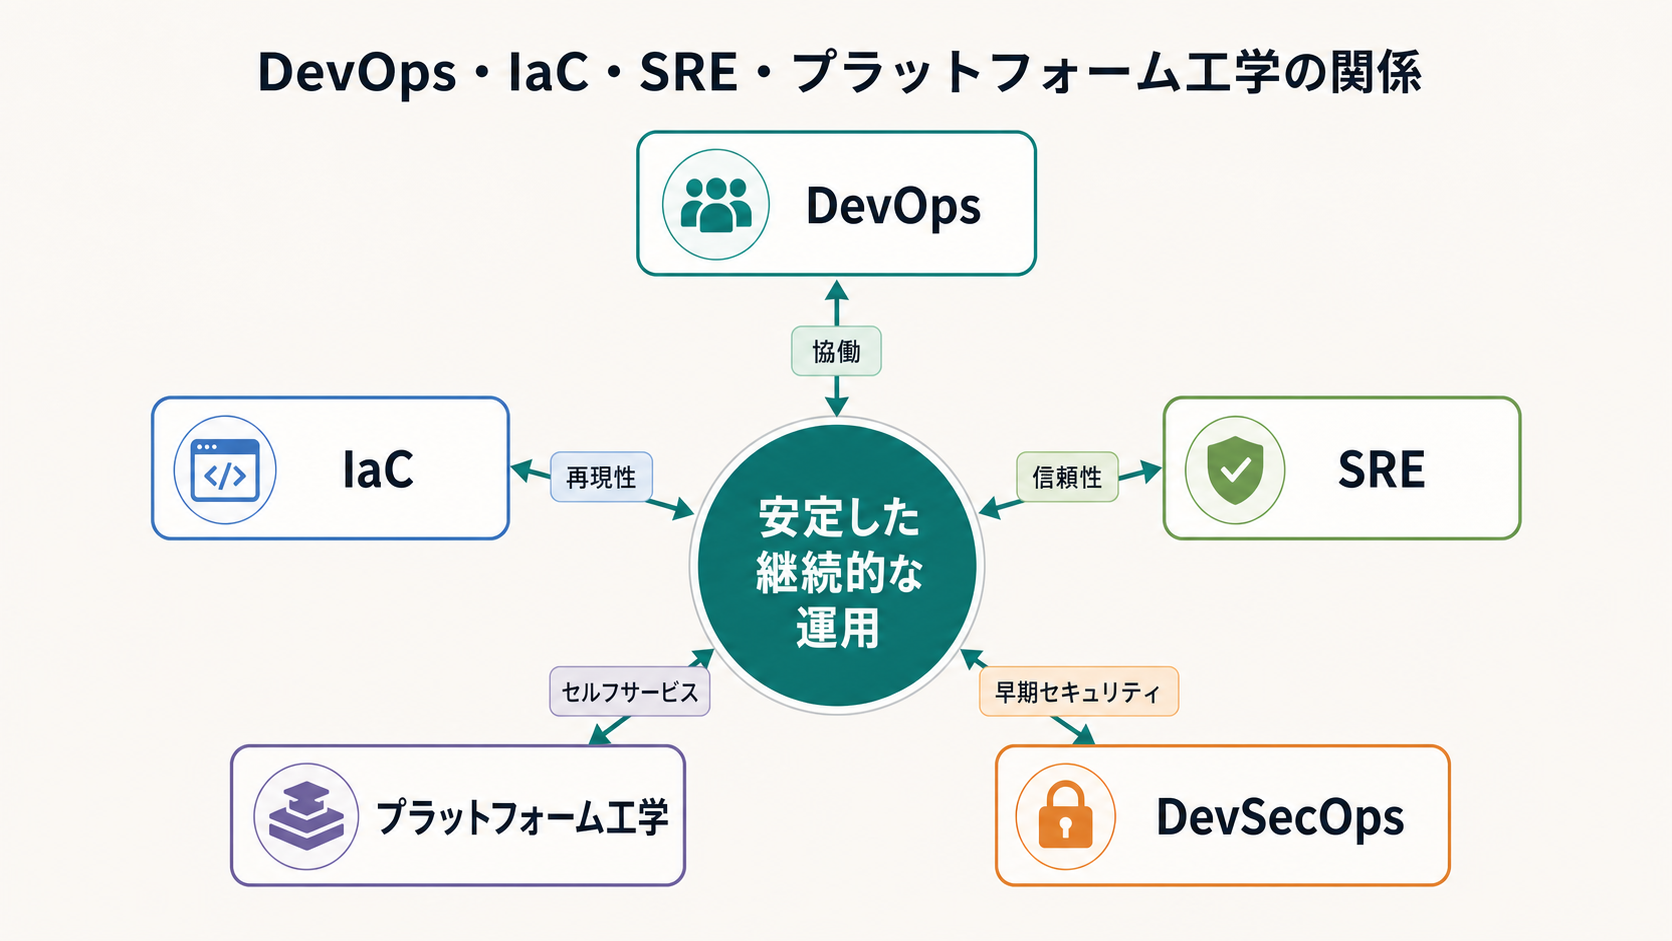
\includegraphics[width=0.96\linewidth]{assets/generated_figures/ch06/fig-ch06-06.png}}{\fbox{\parbox[c][48mm][c]{0.9\linewidth}{\centering 画像生成待ち\\DevOps・IaC・SRE・プラットフォーム工学の関係}}}
\caption{DevOps・IaC・SRE・プラットフォーム工学の関係}
\label{fig:ch06-06}
\end{figure}

\subsection{ソフトウェアエンジニアリング運用提供}

運用提供は、計画された運用サービスを実際に実行し、ソフトウェアを本番利用に耐える形で届ける活動である。ここでは、運用テスト、配備、リリース、ロールバック、データ移行、問題解決が中心となる。

\subsubsection{運用テスト、検証、受け入れ}

運用テストは、ソフトウェアが本番環境または本番に近い環境で運用可能かを確認する活動である。検証は「仕様どおりか」を確認する活動であり、受け入れは「利用者や運用者が使えると判断できるか」を確認する活動である。

現代の運用では、テストは最後に一回だけ行うものではない。テスト駆動開発（TDD）や受け入れテスト駆動開発（ATDD）を使い、開発中から継続的に検証を行う。DevOpsでは、試験サービスや試験ツールを自動化し、開発者が変更のたびに素早く結果を得られるようにする。

\subsubsection{配備・リリース工学}

配備とは、指定された版のソフトウェアを、特定の環境へインストールすることである。リリースとは、機能または機能集合を、顧客や利用者が実際に使える状態にすることである。配備とリリースは似ているが、同じではない。配備は技術的な配置であり、リリースは利用可能にする判断である。

\par\smallskip\noindent\refstepcounter{table}\label{tab:ch06-06}\textbf{表 \thetable: 第06章 ソフトウェアエンジニアリング運用 表06}\par\smallskip
\begin{longtable}{L{35mm}L{115mm}}
\toprule
概念 & 説明 \\
\midrule
配備 & コード、設定、データベース、サーバ、コンテナなどを対象環境へ置き、動作可能にする技術的活動である。 \\
リリース & 配備済みの機能を、すべての利用者または一部の利用者に使えるようにする活動である。ビジネス判断を含む。 \\
\bottomrule
\end{longtable}

従来は、開発チームが完成物を運用チームに引き渡し、運用チームが手作業で配備することが多かった。この方法は時間がかかり、品質面でもリスクがある。DevOpsでは、コードの包装、設定ファイル生成、サーバ再起動、サーバとデータベースの設定、ソフトウェアのインストール、アプリケーション起動、スモークテストを自動化する。

リリース戦略には、環境に基づく戦略とアプリケーションに基づく戦略がある。環境に基づく戦略では、新版を事前本番環境や別環境へ配備してから切り替える。アプリケーションに基づく戦略では、機能トグルのような設定により、コード中の特定機能を有効化または無効化する。

カナリアリリースは、変更を一部の範囲にだけ短期間配備し、その結果を評価してから全面配備を判断する方法である。新しいソフトウェアが異常を示した場合、自動的にロールバックできる構成も重要である。

\begin{figure}[htbp]
\centering
\IfFileExists{assets/generated_figures/ch06/fig-ch06-07.png}{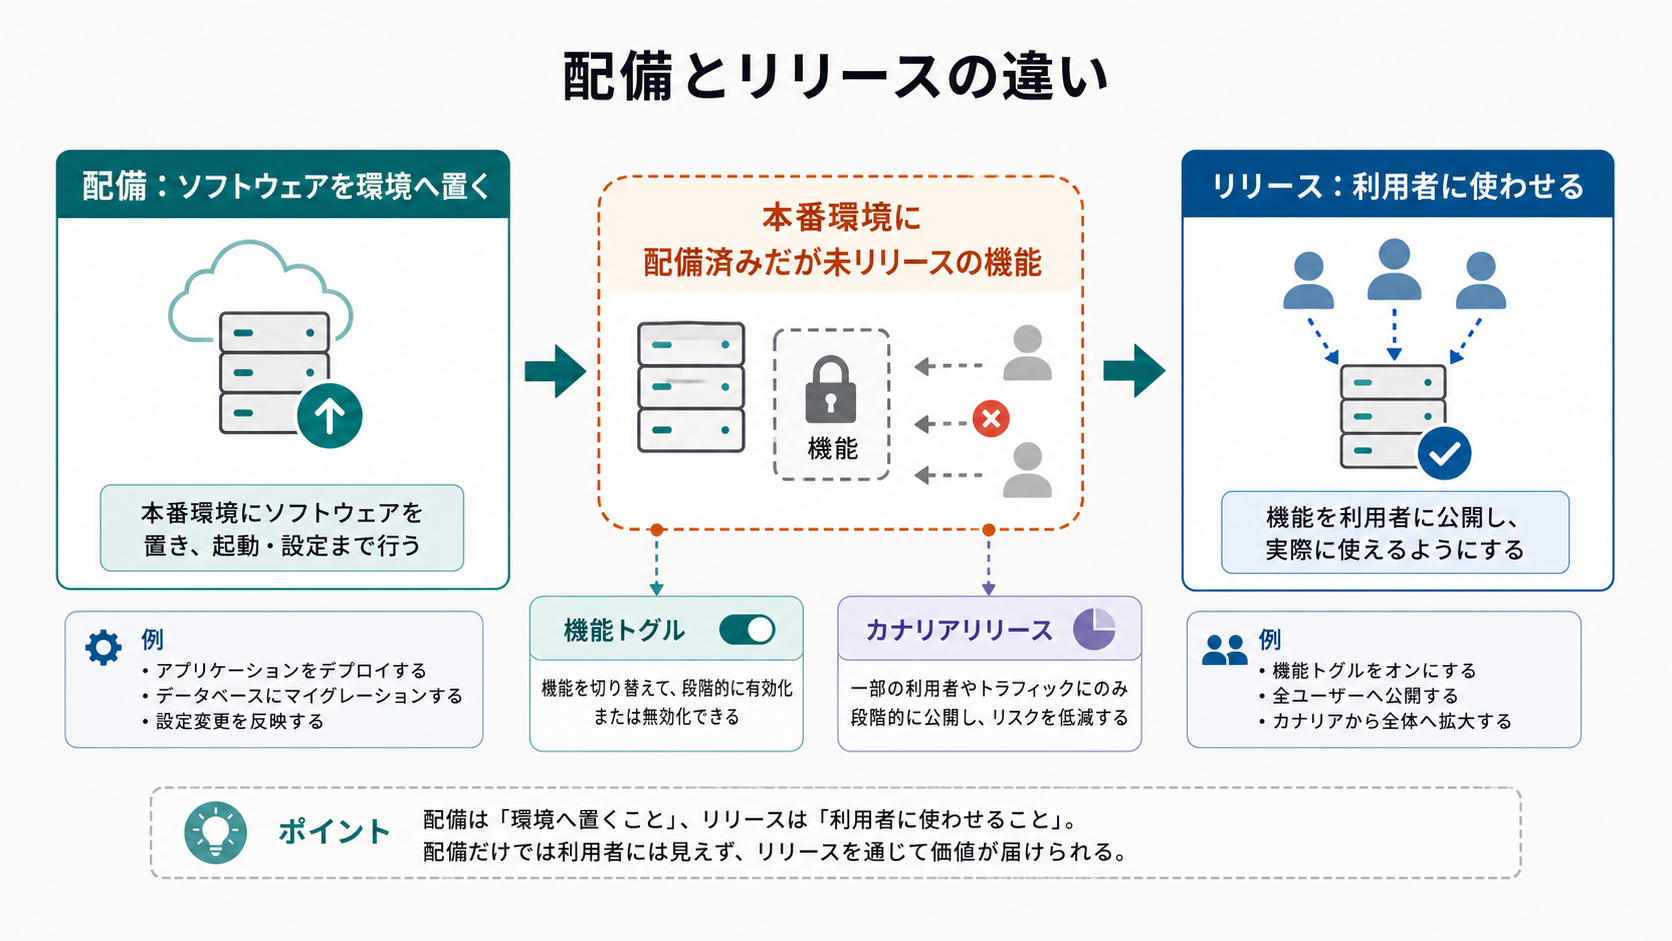
\includegraphics[width=0.96\linewidth]{assets/generated_figures/ch06/fig-ch06-07.png}}{\fbox{\parbox[c][48mm][c]{0.9\linewidth}{\centering 画像生成待ち\\配備とリリースの違い}}}
\caption{配備とリリースの違い}
\label{fig:ch06-07}
\end{figure}

\subsubsection{ロールバックとデータ移行}

ロールバックとは、新しい版のソフトウェアやデータベースが問題を起こしたとき、正しく動く以前の状態へ戻す活動である。データ移行とは、ソフトウェア変更に合わせてデータ構造や内容を移す活動である。

本番配備前には、ロールバック手順が計画され、練習されるべきである。新しい版が障害や性能劣化を起こした場合、素早く以前の状態へ戻せる必要がある。DevOpsでは、この過程を自動化し、監視結果に応じて自動的に戻すことも可能である。

データ移行がある場合、単にプログラムを戻すだけでは不十分である。データの形式が変わっていると、旧版が新しいデータを読めないことがある。したがって、ロールバック計画には、データをどの状態に戻すか、どこまでの処理を再実行するか、利用者にどの影響があるかを含める必要がある。

\begin{figure}[htbp]
\centering
\IfFileExists{assets/generated_figures/ch06/fig-ch06-08.png}{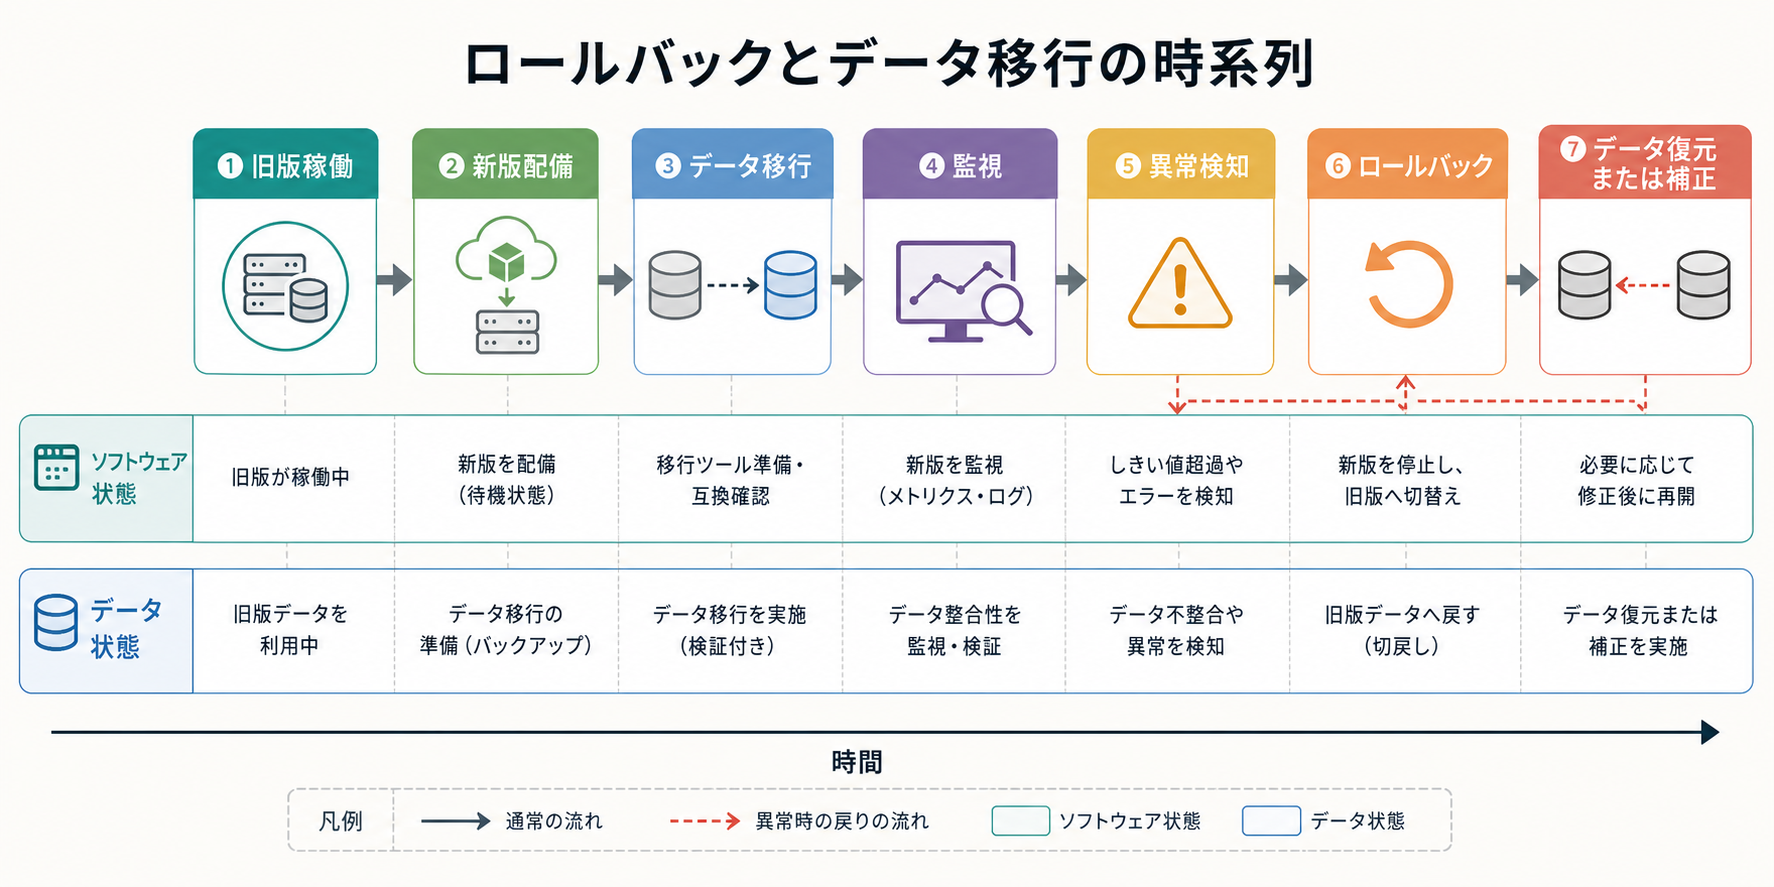
\includegraphics[width=0.96\linewidth]{assets/generated_figures/ch06/fig-ch06-08.png}}{\fbox{\parbox[c][48mm][c]{0.9\linewidth}{\centering 画像生成待ち\\ロールバックとデータ移行の時系列}}}
\caption{ロールバックとデータ移行の時系列}
\label{fig:ch06-08}
\end{figure}

\subsubsection{問題解決}

問題解決は、ソフトウェアやシステムのインシデントと問題の原因を識別し、分析し、事業への混乱を最小化する活動である。繰り返し発生する本番問題には、ソフトウェア、インフラ、設定、データベース、ネットワーク、人間の手順など、複数の原因が絡むことがある。そのため、問題解決には、ソフトウェア技術者、運用担当技術者、セキュリティ担当、データベース担当、製品責任者などの多職種チームが必要になる場合がある。

問題解決では、監視、ログ、プロファイル、実行トレース、設定履歴を使って、何が起きたか、いつ起きたか、どの変更と関係するかを調べる。問題の根本原因がわかれば、再発防止策を実装する。

\subsection{ソフトウェアエンジニアリング運用制御}

運用制御は、運用中のサービスを観察し、制御し、問題に対応し、変更を管理し、結果を報告する活動である。運用は一度設定すれば終わりではない。利用者、負荷、脅威、法規制、事業要求、技術基盤は変化する。その変化を制御しなければ、サービス品質は低下する。

\subsubsection{インシデント管理}

インシデント管理とは、ソフトウェアインシデントを記録し、優先順位を付け、事業影響を評価し、解決、エスカレーション、終了まで管理するプロセスである。

現代のDevOpsでは、アラートとログを用いた監視を自動化し、小さなインシデントが大きな障害になる前に検出する。インシデントが発生したら、原因を分析し、事後検討を行い、同じインシデントを繰り返さないための対策を実施する。

\subsubsection{変更管理}

変更管理とは、すべての変更を評価、承認、実装、レビューされた状態で行うためのプロセスである。変更要求は記録され、緊急、至急、重大、軽微などに分類される。変更管理では、変更のリスク、ロールバック戦略の必要性、関係者への通知、変更スケジュールを扱う。

従来型の開発では、多くの変更をまとめて定期リリースとして提供することが多かった。DevOpsでは、小さな変更単位を独立に、必要に応じて届けることを目指す。そのためには、ソフトウェアが小さく独立した配備に向くように設計されている必要がある。

\subsubsection{監視、測定、追跡、レビュー}

運用では、容量、継続性、可用性を監視する。DevOpsの考え方では、希望的観測に頼ってはならない。システム品質と運用状態を、証拠に基づいて判断する必要がある。

\par\smallskip\noindent\refstepcounter{table}\label{tab:ch06-07}\textbf{表 \thetable: 第06章 ソフトウェアエンジニアリング運用 表07}\par\smallskip
\begin{longtable}{L{55mm}L{95mm}}
\toprule
測定対象 & 意味 \\
\midrule
本番システム監視と製品テレメトリ & 本番で何が起きているかを示す。ログ、トレース、利用者行動、資源使用量などを含む。 \\
リリース前後の検証結果 & リリースが期待どおりに動くか、リリース後に品質が悪化していないかを示す。 \\
利用者活動と資源使用 & どの機能が使われ、どの資源が消費されているかを示す。 \\
影響分析結果 & ある変更がどの機能、構成、利用者に影響するかを示す。 \\
依存関係 & サービス運用に必要な内部依存と外部依存を示す。 \\
構成変更 & 承認済み配備以外の設定変更や環境差分を検出する。 \\
セキュリティと耐障害性 & 攻撃、障害、復旧に対する能力を示す。 \\
\bottomrule
\end{longtable}

\begin{figure}[htbp]
\centering
\IfFileExists{assets/generated_figures/ch06/fig-ch06-09.png}{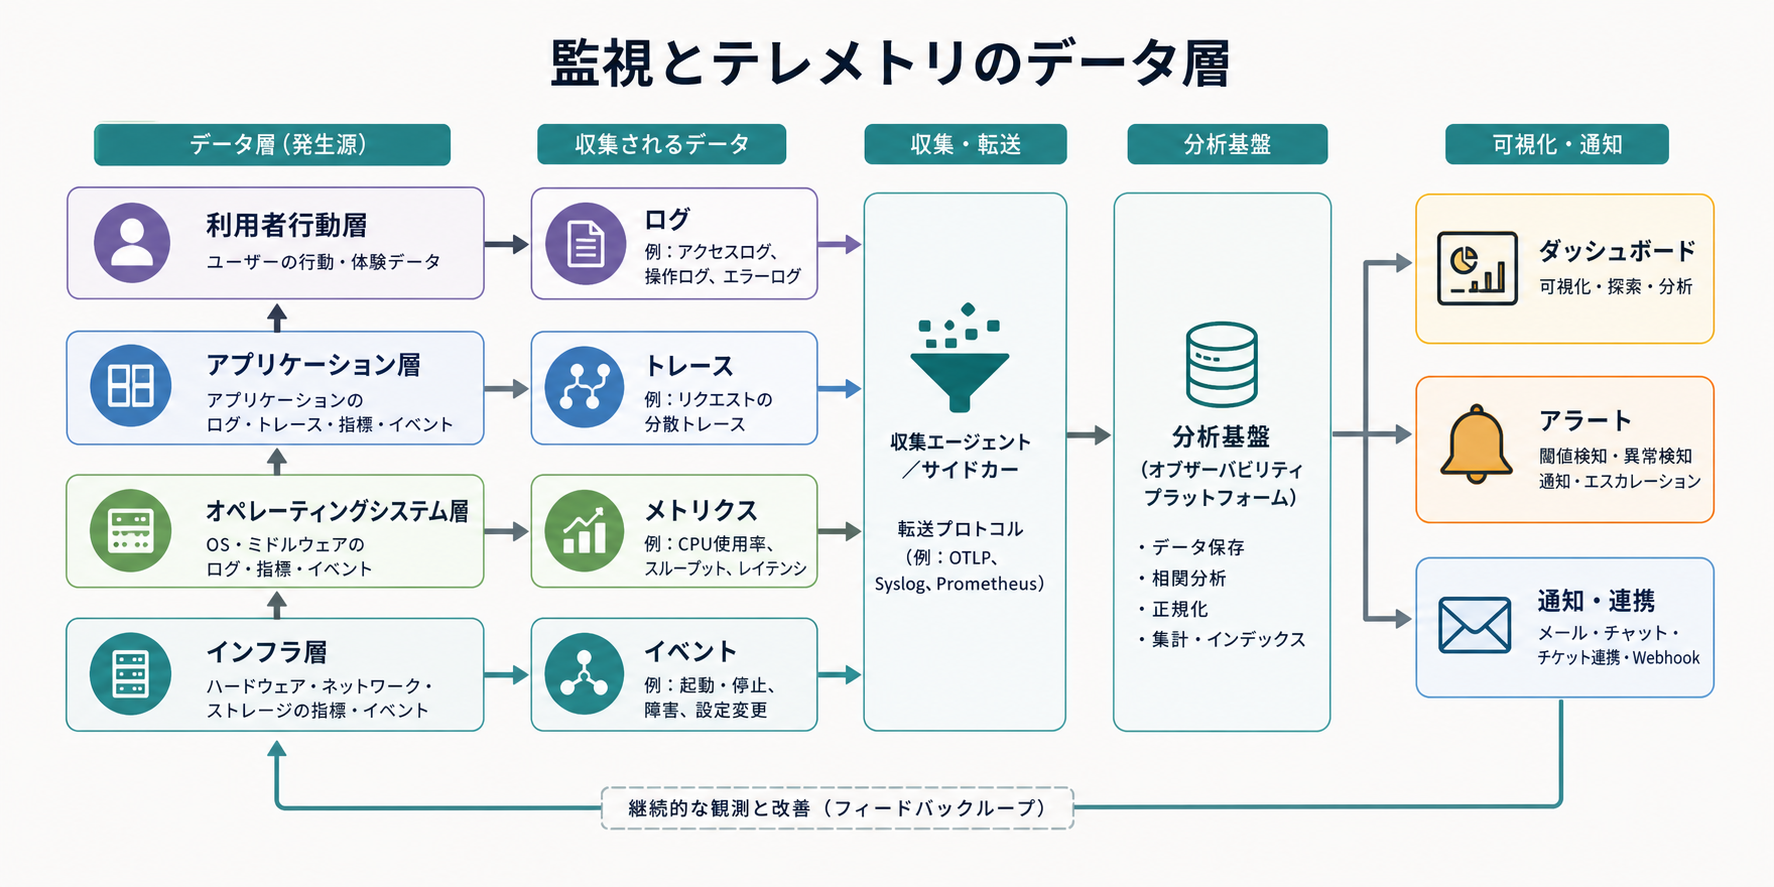
\includegraphics[width=0.96\linewidth]{assets/generated_figures/ch06/fig-ch06-09.png}}{\fbox{\parbox[c][48mm][c]{0.9\linewidth}{\centering 画像生成待ち\\監視とテレメトリのデータ層}}}
\caption{監視とテレメトリのデータ層}
\label{fig:ch06-09}
\end{figure}

\subsubsection{運用支援}

運用支援は、ソフトウェア製品を意図された環境で動かし、顧客や利用者を支援する活動である。運用支援はプロジェクトの計画段階から始まり、実行段階では監視、イベント対応、インシデント対応、問い合わせ対応、手順実行、運用文書更新を行う。

運用支援活動はSLAに記述されることが多い。たとえば、サポート時間、初動応答時間、障害の重大度分類、復旧目標、報告形式、エスカレーション経路などである。

\subsubsection{サービス報告}

サービス報告は、意思決定に必要な、合意済みで、適時で、信頼でき、正確な情報を作る活動である。報告は、運用サービスがどのように機能したか、サービス水準を満たしたか、どの問題が発生したか、今後の傾向がどうかを示す。

典型的な報告項目には、サービス水準目標に対する性能、セキュリティ侵害、トランザクション量、資源使用量、インシデントと失敗、傾向情報、満足度分析がある。測定を自動化し、収集、分析、報告、制御を調整できる枠組みとツールを選定することが重要である。

\begin{figure}[htbp]
\centering
\IfFileExists{assets/generated_figures/ch06/fig-ch06-10.png}{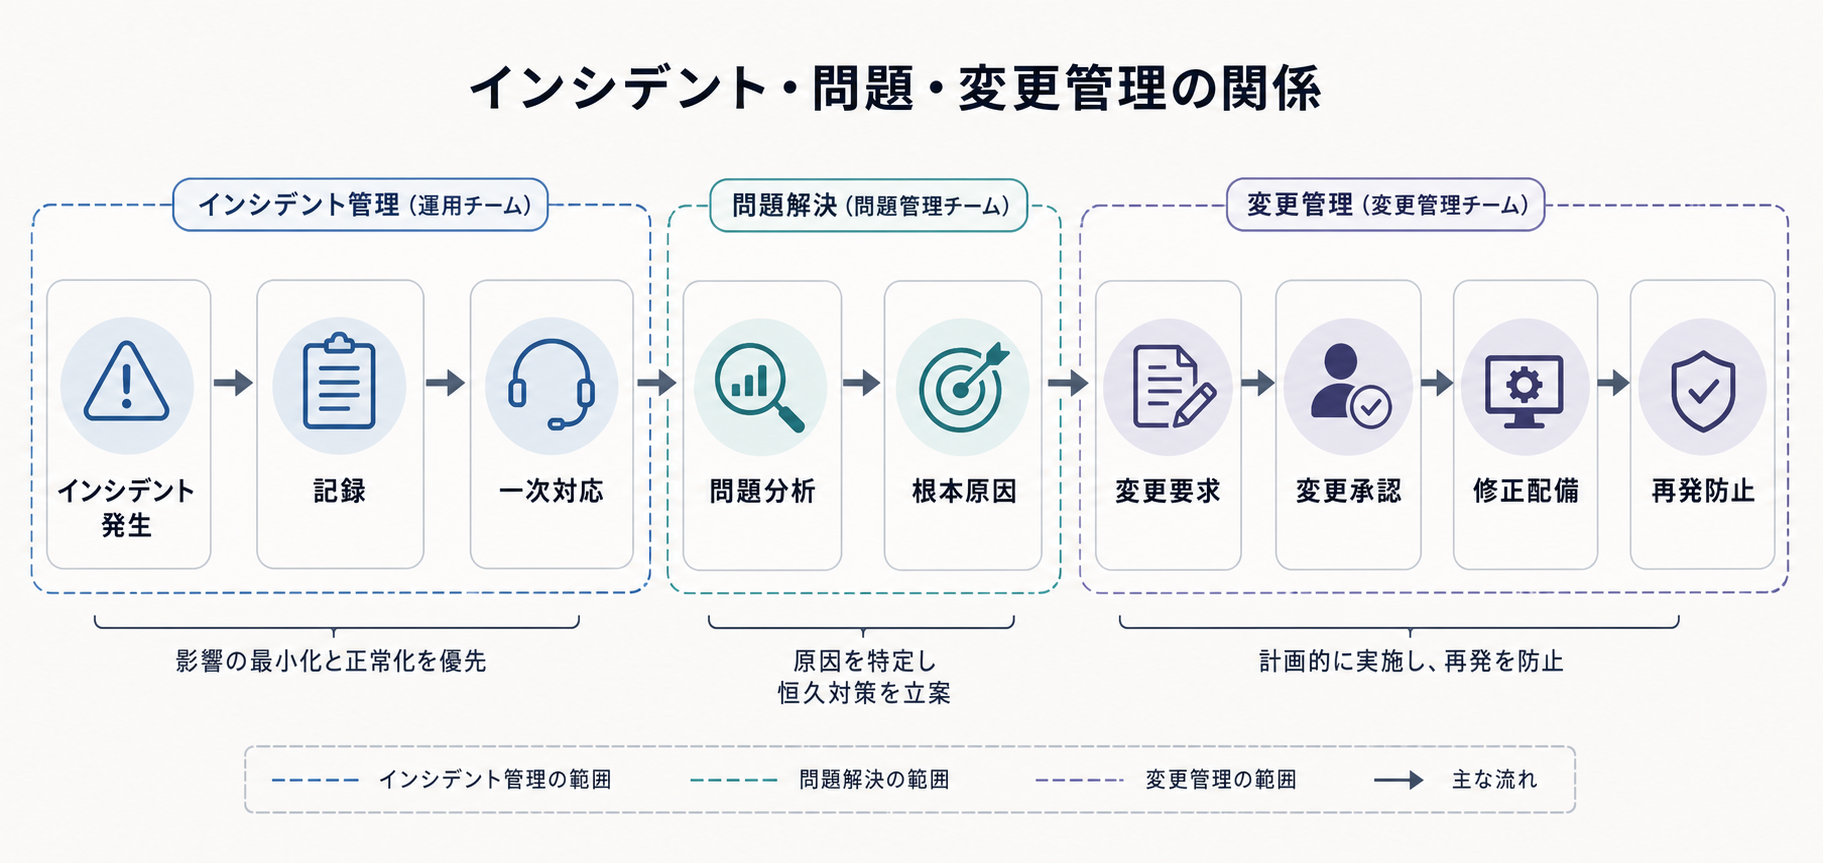
\includegraphics[width=0.96\linewidth]{assets/generated_figures/ch06/fig-ch06-10.png}}{\fbox{\parbox[c][48mm][c]{0.9\linewidth}{\centering 画像生成待ち\\インシデント・問題・変更管理の関係}}}
\caption{インシデント・問題・変更管理の関係}
\label{fig:ch06-10}
\end{figure}

\subsection{実務上の考慮}

\subsubsection{インシデントと問題の予防}

インシデントや問題を予防するには、運用プロセス全体を可能な限り自動化し、試験を継続的に統合する必要がある。さらに、製品テレメトリを適切な分析技法と組み合わせ、問題を早期に検出する。

データは、アプリケーション層、オペレーティングシステム層、インフラ層など、製品スタックのすべての層から収集されるべきである。テレメトリは、問題の兆候を発見するだけでなく、問題源を特定するための基盤になる。

\subsubsection{運用リスク管理}

運用担当技術者は、可用性、拡張性、セキュリティ、個人情報漏えい、誤配備、容量不足、外部サービス停止など、多くのリスクを管理する。継続的リスク管理では、運用状態を常に監視し、リスクを検出したら自動的にアラートを出す。

何をアラートにするかは、製品責任者やソフトウェア技術者と相談して、リスク許容度を定める必要がある。すべての小さな変化で警報を出すと、警報疲れが起こる。逆に、重大な兆候を見逃すと、障害や事故につながる。

\subsubsection{ソフトウェアエンジニアリング運用の自動化}

現代の運用では、自動化が中心的役割を持つ。環境構築、ユーザアカウント作成、サーバ準備、実行時設定変更、配備、試験、デバッグ支援などを自動化できる。ソフトウェア技術者は、アプリケーション自動化と運用自動化を結びつけることで大きな効果を得る。

運用自動化の傾向は、複雑さを減らし、インフラ準備を速め、開発者へ運用サービススクリプトを提供し、アプリケーション定義、配備、試験作業を自動化する方向にある。

\begin{figure}[htbp]
\centering
\IfFileExists{assets/generated_figures/ch06/fig-ch06-11.png}{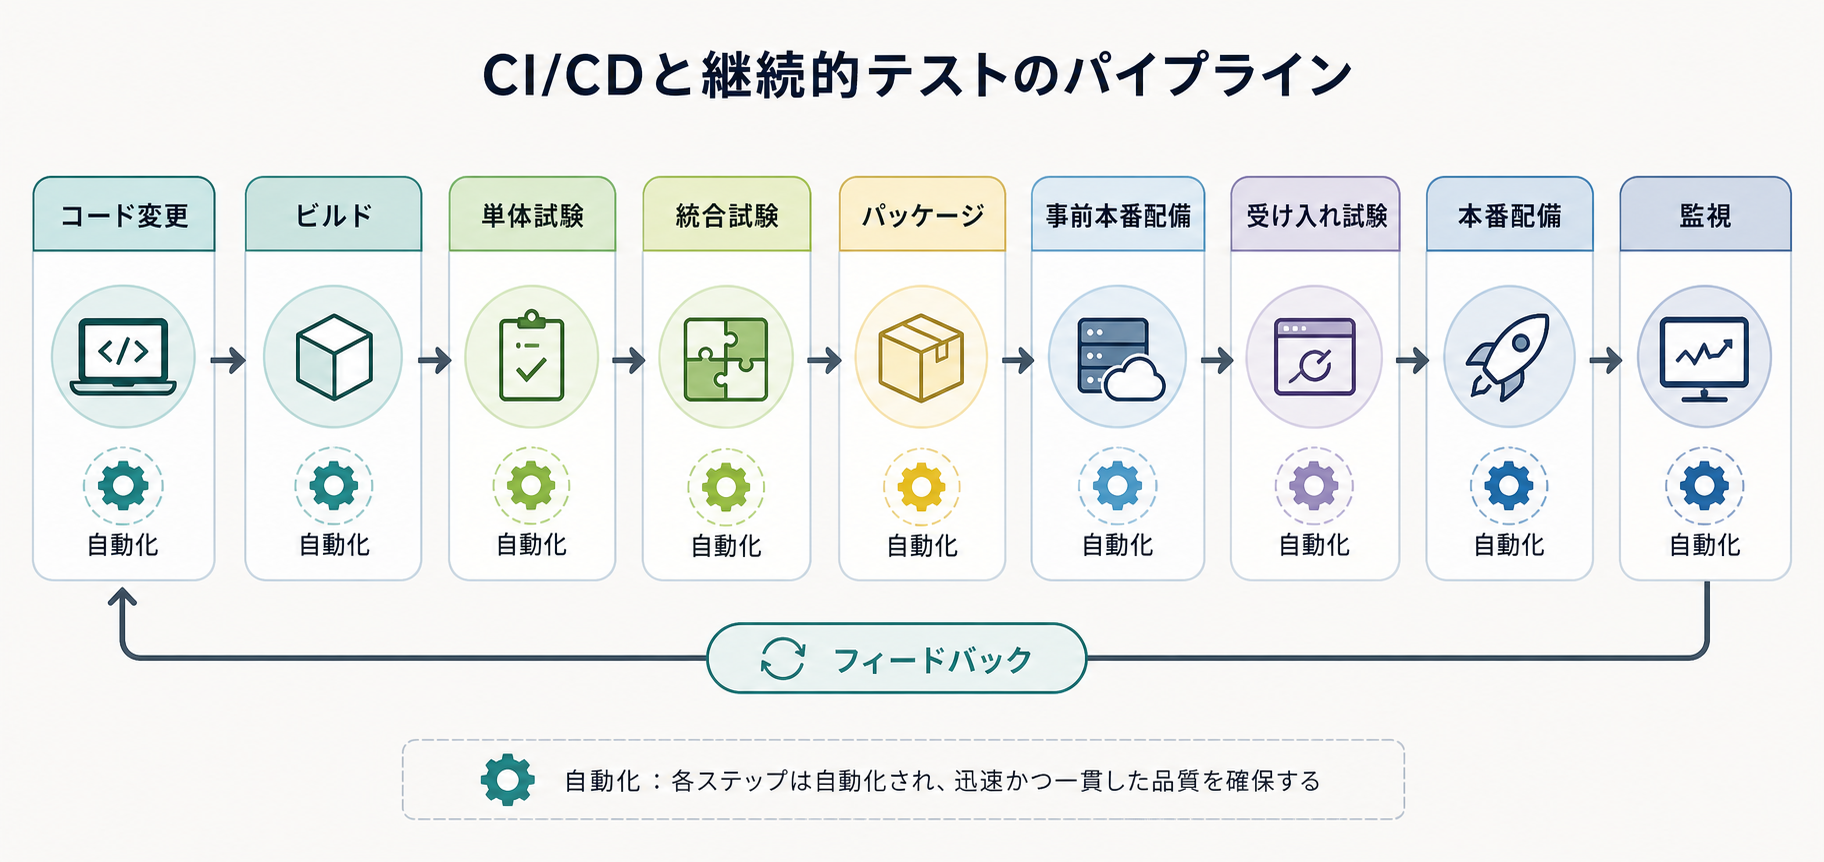
\includegraphics[width=0.96\linewidth]{assets/generated_figures/ch06/fig-ch06-11.png}}{\fbox{\parbox[c][48mm][c]{0.9\linewidth}{\centering 画像生成待ち\\CI/CDと継続的テストのパイプライン}}}
\caption{CI/CDと継続的テストのパイプライン}
\label{fig:ch06-11}
\end{figure}

\subsubsection{小規模組織における運用}

小規模組織、とくに25人以下の非常に小さい組織では、大規模組織向けの標準をそのまま適用することが難しい。標準が要求する文書、役割、手順、監査が過大になることがある。この場合、小規模組織向けに調整されたISO/IEC 29110系列のような指針が有用である。

重要なのは、小規模であることを理由に運用を無視しないことである。むしろ、少人数だからこそ、自動化、標準化、簡潔な手順、明確な責任分担が重要になる。小規模組織では、最小限のSLA、バックアップ手順、インシデント対応、変更管理、監視ダッシュボードから始めるとよい。

\subsection{ソフトウェアエンジニアリング運用ツール}

運用ツールは、人的資源を効率よく使い、品質と応答速度を高めるために重要である。適切に実装された自動化は、手作業より速く、容易で、信頼性が高い。DevOpsでは、開発、保守、運用の資源と手順を結びつけ、継続的インテグレーション、継続的デリバリー、継続的テスト、継続的デプロイを支援する。

継続的デリバリーは、新しいシステムやソフトウェアを頻繁に試験環境や事前本番環境へ届ける実践である。継続的テストは、ソフトウェアライフサイクルの各段階で品質を評価する実践である。継続的デプロイは、自動検証を通過した変更を本番へ自動配備するプロセスである。

\subsubsection{コンテナと仮想化}

コンテナと仮想化は、アプリケーションの拡張性を高め、複数のサーバやクラウド提供者にまたがる配備を標準化するために使われる。コンテナは、アプリケーションと実行に必要な依存関係をまとめ、環境差分を減らす。仮想化は、物理サーバ上に複数の仮想サーバを作る。

運用担当技術者は、プロジェクトの規模、複雑さ、柔軟性、セキュリティ、監視要求に基づいてツールを選ぶ。コンテナ管理ツール、すなわちオーケストレータは、多数のコンテナの配備、再起動、スケーリング、ネットワーク、監視を支援する。

\subsubsection{配備}

配備ツールは、さまざまな環境へのソフトウェア配備を管理する。配備記述ファイル、設定ファイル、環境変数、シークレット管理、コンテナイメージ、クラウド資源、データベース変更などを扱う。

実務では、一つのツールだけで全体をまかなうことは少ない。ビルド、パッケージ、インフラ作成、設定管理、データベース移行、監視、アラート、ロールバックなど、複数のツールを組み合わせて配備パイプラインを構築する。

\subsubsection{自動テスト}

開発者へ速く継続的なフィードバックを提供するため、テストはソフトウェア提供プロセス全体で可能な限り自動化されるべきである。単体試験、統合試験、システム試験、利用者受け入れ試験を含む試験戦略を定義し、それぞれを支援するツールを選ぶ。

自動テストは、単に欠陥を検出するだけではない。変更が安全に本番へ進めるかを判断する門番である。自動テストが不十分だと、配備を速くするほど障害を速く広げてしまう。

\subsubsection{監視とテレメトリ}

監視とテレメトリは、運用の中核である。監視は、サービスが正常かどうかを観察する活動である。テレメトリは、システムからデータを収集して分析に使う仕組みである。

監視では、アプリケーション層のログ、オペレーティングシステム層の実行トレース、サーバ層のCPU使用量やメモリ使用量などを収集する。収集されたデータには、統計分析や機械学習を使って意味を抽出できる。最終的には、ダッシュボードにより、開発者、運用者、製品責任者、経営層など、異なる利害関係者に必要な情報を見せる。

\begin{figure}[htbp]
\centering
\IfFileExists{assets/generated_figures/ch06/fig-ch06-12.png}{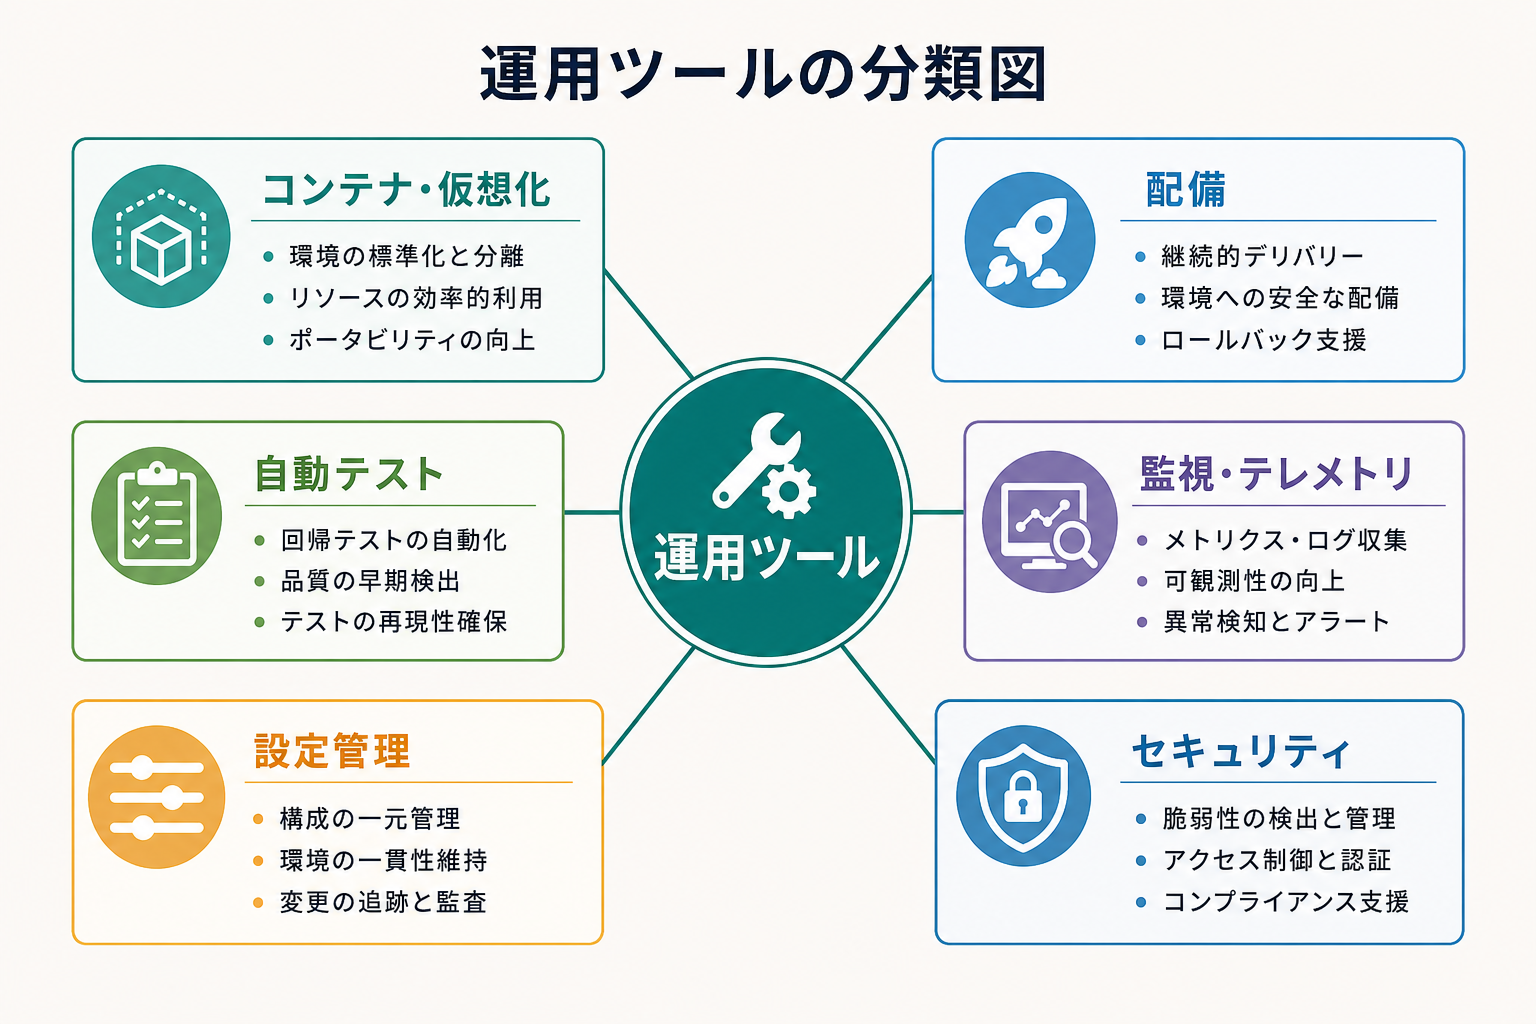
\includegraphics[width=0.96\linewidth]{assets/generated_figures/ch06/fig-ch06-12.png}}{\fbox{\parbox[c][48mm][c]{0.9\linewidth}{\centering 画像生成待ち\\運用ツールの分類図}}}
\caption{運用ツールの分類図}
\label{fig:ch06-12}
\end{figure}

\subsection{トピックと参考文献の対応}

この表は、SWEBOK 06章のトピックと主要参考資料を、学習用に簡略化したものである。

\par\smallskip\noindent\refstepcounter{table}\label{tab:ch06-08}\textbf{表 \thetable: 第06章 ソフトウェアエンジニアリング運用 表08}\par\smallskip
\begin{longtable}{L{70mm}L{80mm}}
\toprule
トピック & 主な参考資料 \\
\midrule
ソフトウェアエンジニアリング運用の基礎 & ISO/IEC/IEEE 20000-1、ISO/IEC/IEEE 12207、The DevOps Handbook \\
運用プロセス & ISO/IEC/IEEE 20000-1、ISO/IEC/IEEE 12207、ISO/IEC/IEEE 32675 \\
ソフトウェア導入、スクリプト化、自動化 & The DevOps Handbook、ISO/IEC/IEEE 20000-1 \\
テストとトラブルシューティング & The DevOps Handbook、ソフトウェアテスト知識領域 \\
性能、信頼性、負荷分散 & ISO/IEC/IEEE 20000-1、SRE文献 \\
運用計画と供給者管理 & ISO/IEC/IEEE 20000-1、ISO/IEC/IEEE 12207 \\
開発環境と運用環境 & The DevOps Handbook、IaC関連標準 \\
可用性、継続性、サービス水準 & ISO/IEC/IEEE 20000-1、ソフトウェア保守知識領域 \\
容量管理 & ISO/IEC/IEEE 20000-1 \\
バックアップ、災害復旧、フェイルオーバー & ISO/IEC/IEEE 20000-1、SRE文献 \\
安全性、セキュリティ、完全性、保護、統制 & ISO/IEC/IEEE 20000-1、ISO/IEC/IEEE 32675、ソフトウェアセキュリティ知識領域 \\
配備・リリース工学 & The DevOps Handbook、Continuous Delivery、ソフトウェア構成管理知識領域 \\
ロールバックとデータ移行 & The DevOps Handbook、ISO/IEC/IEEE 12207 \\
インシデント管理、変更管理、問題解決 & ISO/IEC/IEEE 20000-1、The DevOps Handbook \\
監視、測定、追跡、レビュー & The DevOps Handbook、The Art of Monitoring \\
小規模組織における運用 & ISO/IEC 29110系列 \\
運用ツール & The DevOps Handbook、The Art of Monitoring、ISO/IEC/IEEE 32675 \\
\bottomrule
\end{longtable}

\subsection{参考文献}

\begin{enumerate}[label={\arabic*.}]
  \item ISO/IEC/IEEE 20000-1:2013, Information technology -- Service management -- Part 1: Service management systems requirements.
  \item G. Kim, J. Humble, J. Debois, J. Willis, and N. Forsgren, \textit{The DevOps Handbook: How to Create World-Class Agility, Reliability and Security in Technology Organizations}, 2nd ed., IT Revolution Press, 2021.
  \item ISO/IEC/IEEE 12207:2017, Systems and software engineering -- Software Life Cycle Processes.
  \item ISO/IEC/IEEE 32675:2022, Information Technology -- DevOps: Building Reliable and Secure Systems Including Application Build, Package and Deployment.
  \item ISO/IEC/IEEE 24765:2017, Systems and Software Engineering -- Vocabulary, 2nd ed., 2017.
  \item B. Beyer, C. Jones, J. Petoff, and N. R. Murphy, \textit{Site Reliability Engineering: How Google Runs Production Systems}, O'Reilly Media, 2016.
  \item ISO/IEC CD 29110-5-5:2023, Systems and software engineering -- Lifecycle profiles for Very Small Entities, Part 5-5: Agile/DevOps guidelines.
  \item J. Humble and D. Farley, \textit{Continuous Delivery: Reliable Software Releases through Build, Test, and Deployment Automation}, Pearson Education, 2010.
  \item J. Turnbull, \textit{The Art of Monitoring}, James Turnbull, 2016.
\end{enumerate}

\subsection{章末確認問題}

\begin{enumerate}
  \item ソフトウェアエンジニアリング運用は、単なる本番配備とどう違うか。
  \item 運用計画、運用提供、運用制御の違いを説明せよ。
  \item 運用担当技術者とソフトウェア技術者の役割の違いを説明せよ。
  \item IaCが環境差分を減らす理由を説明せよ。
  \item 配備とリリースの違いを、具体例を使って説明せよ。
  \item カナリアリリースがリスクを減らす理由を説明せよ。
  \item ロールバック計画にデータ移行が含まれるべき理由を説明せよ。
  \item インシデント管理、問題解決、変更管理の関係を説明せよ。
  \item 監視とテレメトリが、インシデント予防に役立つ理由を説明せよ。
  \item 小規模組織では、どの運用活動から始めるのが現実的かを述べよ。
\end{enumerate}

\begin{pointbox}{解答の方向性}
1は、配備、設定、監視、障害対応、変更管理、容量管理、バックアップ、復旧、セキュリティを含む点を述べる。2は、計画が準備、提供が実行、制御が監視と管理である点を述べる。5は、配備は環境へ置くこと、リリースは利用者に使わせることと説明する。8は、インシデントを記録し、問題として原因を分析し、変更管理で修正を安全に入れる流れとして説明できる。
\end{pointbox}

\end{document}

